\pdfbookmark[0]{Viertes Buch.}{viertesbuch}
\pdfbookmark[1]{I. Capitel.}{IV.I.Capitel}
\cehead{\edins{{{\large IV,}} I. Ihre Aufgaben.}}
\cohead{ }
\chapter*{Viertes Buch.}\phantomsection\label{IV}
\section*{Die allgemeine Sprachwissenschaft}
\section*{I. Capitel.}\phantomsection\label{IV.I}
\section*{Ihre Aufgaben.}

\fed{{\textbar}292{\textbar}}\phantomsection\label{fp.292} \sed{{\textbar}{\textbar}302{\textbar}{\textbar}}\phantomsection\label{sp.302}

Thatsächlich befinden wir uns längst mitten drin in der allgemeinen Sprachwissenschaft. Was ich von der einzelsprachlichen Forschung gesagt habe, gilt, wenn anders es richtig ist, nicht nur von dieser oder jener, sondern von allen Einzelsprachen. Und die Grundsätze der historisch-genealogischen Forschung wollen nicht nur für eine einzelne Sprachfamilie, sondern für alle gelten. Auch waren die Erkenntnisse, zu denen wir gelangten, nicht diesem oder jenem beschränkten Sprachgebiete abgewonnen, sondern sie beruhten entweder auf der Natur der Sache oder auf einem möglichst weiten Kreise von Erfahrungen. Für jene begrenzteren Forschungen beanspruchen sie eigentlich nur hodegetischen Werth: sie zeigen, was der Forscher bei seinen Arbeiten wahrzunehmen, und worauf er unter Umständen gefasst zu sein habe.

Offenbar ist hiermit die Aufgabe der allgemeinen Sprachwissenschaft noch nicht erschöpft. Diese Wissenschaft hat das menschliche Sprachvermögen selbst zum Gegenstande. Sie will dies Vermögen begreifen, nicht nur in Rücksicht auf die geistleiblichen Kräfte und Anlagen, aus denen es sich zusammensetzt, sondern auch, soweit dies erreichbar ist, \update{in dem}{dem} ganzen Umfange seiner Entfaltungen.

Es handelt sich zunächst um ein Begreifen, das heisst um ein Zurückführen auf Gründe. Wir wollen wissen: Wie kommt die Menschheit zur Sprache? warum hat sie ihre Sprachen so \update{mannich\-faltig}{mannig\-faltig} entwickelt? Bald aber wird es sich zeigen, dass diese Sprachen nicht nur Gebilde, sondern auch Bildnerinnen der Völker sind; und dann werden \fed{{\textbar}293{\textbar}}\phantomsection\label{fp.293} wir weiter fragen müssen: Welchen Antheil haben sie an der geistigen Entwickelung der Völker? worauf beruht ihr verschiedener Werth? Jetzt gilt es nicht mehr der Herkunft, sondern es gilt den Wirkungen, al\-so dem Werthe der Sprachen, nicht mehr den Mächten \sed{{\textbar}{\textbar}303{\textbar}{\textbar}}\phantomsection\label{sp.303} und Schicksalen, durch die sie so geworden, wie sie sind, sondern den Kräften, die sie zugleich äussern und wecken.

Endlich wird immer und immer wieder das Bestreben auftauchen, sei es rückschliessend, sei es durch apriorische Speculation, ein Bild von dem Urzustande menschlicher Rede zu gewinnen. Der Sehnsucht nach einem Einblicke in die ersten Anfänge alles Seienden kann sich die Wissenschaft nirgends erwehren.

\pdfbookmark[1]{II. Capitel.}{IV.II.Capitel}
\cehead{{{\large IV,}} II. Die Grundlagen des menschlichen Sprachvermögens.}
\pdfbookmark[2]{§1. Allgemeines.}{IV.II.1}
\cohead{§1. Allgemeines.}
\section*{II. Capitel.}\phantomsection\label{IV.II}
\section*{Die Grundlagen des menschlichen Sprachvermögens.}
\subsection*{§ 1.}\phantomsection\label{IV.II.1}
\subsection*{Allgemeines.}
In physiologischer Hinsicht ist der Mensch ein Säugethier; körperlich steht der Orang-utan, der Chimpanse oder Gorilla dem Menschen näher, als etwa der Katze, dem Elefanten, dem Känguruh, oder gar der Robbe und dem Walfische. Und umgekehrt, in Rücksicht auf das geistige Vermögen steht der Elefant, der gelehrige Hund, der schwatzende Papagei, vielleicht selbst die staatenartig lebende Ameise dem Menschen ebenso nah oder näher, als manche Art der Anthropoiden. Woher nun jener erste unter den Vorzügen des Menschen, die menschliche Sprache?

Offenbar liegt es nicht unserer Wissenschaft ob, sich mit unseren etwaigen sprachlosen Vorfahren zu beschäftigen; für Alalen sind wir recht buchstäblich nicht zu sprechen.

Die Frage, ob die Sprache ein göttliches Geschenk oder ein Erzeugniss der Menschen sei, ist nicht der Aufregung werth, die sie ehemals verursacht hat Die Wissenschaft will und soll das Wunder soweit zurückschieben, das Reich der erkannten Gesetzlichkeit soweit ausdehnen, wie nur immer möglich. Dass etwa der Schöpfer unsern Ureltern eine \fed{{\textbar}294{\textbar}}\phantomsection\label{fp.294} Sprache fix und fertig mit auf den Weg gegeben, oder dass er den Adam in der Art, wie es Genesis 2, 19–20 des Näheren beschrieben wird, zur Benennung der Thierarten veranlasst habe, solche und ähnliche Dinge kann die Sprachwissenschaft von ihrem Standpunkte aus und mit ihren Mitteln weder beweisen noch widerlegen. Fragt sie aber: Gesetzt, es wäre von Alledem nichts geschehen, hatte dann der Mensch in sich die Kraft und den Trieb zur Sprachschöpfung? fragt sie so, dann thut sie nur ihre Schuldigkeit und übt ihr gutes Recht.

\sed{Man hat sonst wohl das Problem anders gefasst; man hat gefragt: Wie} {\textbar}{\textbar}304{\textbar}{\textbar}\phantomsection\label{sp.304} \sed{war die älteste Sprache beschaffen? aus welchen Elementen bestand sie? aus Schallnachahmungen, oder aus Empfindungslauten, etwa aus Schallreflexen, mit denen der Urmensch auf die Eindrücke der Aussenwelt antwortete? Der wissenschaftliche Drang, nach einem einheitlichen letzten Grunde zu suchen, offenbarte sich auch hier, wo er am wenigsten berechtigt war. Die einschlägige Literatur ist sehr umfangreich; und wie alles Mögliche und Unmögliche seine Vertreter findet, ist auch allen Ernstes der Satz verfochten worden: die Schrift sei älter als die Sprache, diese habe sich aus, oder doch an jener entwickelt.}


\begin{styleAnmerk}
\sed{Anmerkung Unter den mir bekannten einschlägigen Büchern dürfte \textsc{H. Stheinthal}’s „Der Ursprung der Sprache“ weitaus das bedeutendste sein. Hier werden auch die wichtigeren Theorien früherer besprochen. Auch \textsc{A. H. Sayce}, Introduction to the Science of Language, chap. 1, giebt eine hübsche Übersicht. Eine weitergehende Beschäftigung mit diesem Zweige der Literatur wird sich der Sprachforscher wohl ohne wesentlichen Nachtheil ersparen können.}
\end{styleAnmerk}

\pdfbookmark[2]{§2. Physische Grundlagen.}{IV.II.2}
\cohead{§2. Physische Grundlagen.}
\subsection*{§. 2.}\phantomsection\label{IV.II.2}
\subsection*{Physische Grundlagen.}
Der Mensch beweist durch Sprache und Gesang eine Fähigkeit zur \update{mannich\-faltig\-sten}{mannig\-faltig\-sten} Laut- und Tonbildung, wie sie in ähnlichem Grade nur gewissen Vogelarten eigen ist. Auf welchen körperlichen Begabungen dies beruht, hat streng genommen nicht die Sprachwissenschaft, sondern die Physiologie zu erklären.

Die Fähigkeit, menschliche Sprachlaute nachzuahmen, besitzen, soviel man bisher weiss, nur wenige Thiere, zumeist Vögel, und unter diesen wieder besonders Papageien und raben- oder krähenartige: Staare, Dohlen, Elstern u. s. w. Doch wurde neuerdings auch von einem sprechenden Canarienvogel berichtet. Unter den Säugethieren sind angeblich die beiden Hausgenossen und Gespielen des Menschen, der Hund und die Katze, in vereinzelten Fällen zum Aussprechen von Wörtern erzogen worden. Man hat aber auch schon des Hundes Gebell für einen Sprechversuch halten wollen, weil verwilderte Hunde mit der Zeit das Bellen verlernen. So scheinen schon hier seelische Mächte mitzuwirken, Umgangsgewohnheiten mit den Neigungen, die aus ihnen folgen. Man hat darauf hingewiesen, dass Hund und Katze gleich den Vögeln und gleich \update{dem}{den} Menschen aufrecht zu sitzen pflegen, also den Brustkasten freier haben, als Thiere, die entweder auf den vier Füssen stehen oder auf dem Bauche liegen. Affen und Eichhörnchen sitzen aber noch menschenähnlicher; denn sie stützen sich nicht einmal auf die vorderen Extremitäten; Beide, zumal die Ersteren, sind oft jahrelang verzogene Lieblinge der Menschen, – und doch hat man meines Wissens von Sprachleistungen der Beiden nie etwas gehört. Hätten etwa doch jene Hausthiere vor den gezähmten das voraus, dass sie seit un\-\sed{{\textbar}{\textbar}305{\textbar}{\textbar}}\phantomsection\label{sp.305}zähligen Reihen von Geschlech\-\fed{{\textbar}295{\textbar}}\phantomsection\label{fp.295}tern zu den Genossen des Menschen gehören und so zu sagen geborene Glieder seiner Familie sind, im Gegensatze zu jenen eingefangenen Gästen?

Viel Einleuchtendes hat es, dass das menschliche Sprachvermögen in einem gewissen Zusammenhange stehe mit derjenigen körperlichen Eigenschaft, die den Menschen am Schärfsten von den übrigen Vertebraten unterscheidet, darin nämlich, dass der Mensch nur die hinteren Extremitäten gebraucht, um sich von der Stelle zu bewegen, die vorderen also zu anderen Zwecken frei hat. Dadurch ist auch die Brust frei, wie beim singenden Vogel, nicht gehemmt durch den Rhythmus der sich bewegenden Extremitäten, wie bei laufenden oder fliegenden Thieren. Und mehr noch: auch der Mund wird durch die Hände von manchen niederen Diensten befreit, dient nicht mehr als greifendes Werkzeug. Und wer mit Fäusten und Knütteln zuschlagen, mit Steinen um sich werfen kann, der braucht die Zähne nur ausnahmsweise als Waffe; wer mit Beilen und Messern arbeitet, braucht das Holz nicht zurechtzunagen, wie der Biber es thut. Die Physiologen mögen entscheiden, ob die Mundorgane durch solche Arbeitsentlastung etwa an Geschmeidigkeit gewinnen, was sie an Kraft verlieren mögen. Sicher gewinnen sie Musse, um sich in der Hervorbringung von Lauten und Tönen zu üben. Und nun können Arme und Hände durch Geberden die gegenseitige Verständigung unterstützen.

Irre ich nicht, so hat man auch das hervorgehoben, dass die tastenden Hände das planimetrische Bild, das die Augen empfangen, so zu sagen stereometrisch berichtigen, den Blick perspectivisch schulen. Allein die Thiere machen ähnliche Erfahrungen, sei es, dass sie die Gegenstände mit den Klauen oder \fed{mit den} Zähnen fassen, sie beschnopern, darauf treten oder liegen. Und mit wie sicherem Augenmasse schätzen sie bei ihren Sprüngen die Entfernung!

Wichtiger dürfte es sein, dass der menschliche Körper, abgesehen von den wahrnehmen den Thätigkeiten, gleichzeitig mehr verschiedene Arbeiten verrichten kann, als wohl irgend ein thierischer. Gehen, dabei mit den Händen eine Frucht abbrechen oder enthülsen und etwa mit dem Munde reden, singen, lachen, schreien: dies, so wenig es zu sein scheint, bringt wohl selbst der Affe nicht zuwege, am Ersten wohl etwa der Elephant, „der Behandete“, wie ihn die Inder nennen; und sollte nicht auch das die Klugheit dieses Dickhäuters gefördert haben? Es ist doch \fed{{\textbar}296{\textbar}}\phantomsection\label{fp.296} immer eine gewisse Vielseitigkeit im Vergleiche mit der einzieligen Gier niederer Thiere.

Vom Gebrauche der Finger als einer natürlichen Rechenmaschine dürfen wir jetzt noch nicht reden. Denn der Geist wäre nicht darauf verfallen, hätte nicht zuvor schon das Zählbedürfniss in ihm gelegen.

Gewicht möchte auf die Nahrung unserer Urväter zu legen sein. Weder ein ausgehungerter Magen noch ein überfüllter giebt die Stimmung zu geistiger \sed{{\textbar}{\textbar}306{\textbar}{\textbar}}\phantomsection\label{sp.306} Arbeit und froher Geselligkeit. Und auch das ist nicht günstig, wenn ein grosser Theil des Tages zum Einnehmen der Nahrung verbraucht wird, wie bei weidenden Grasfressern. Offenbar ist der Mensch in dieser Hinsicht besonders glücklich beanlagt. Fleisch- und Pflanzenkost ist ihm genehm; neben den warmblütigen Thieren verschmäht er auch Fische und Muscheln nicht. Dafür wählt er aber unter den Pflanzen die nahrhafteren, Nüsse, Obst, mehlige Wurzeln und Körner; nur schlechtnährendes Gras und Laub lehnt sein Magen ab. Der Vortheil ist nicht zu unterschätzen. Einmal ist es doch wieder ein Stück jener Vielseitigkeit, die der Vernunftentwickelung zugute kommt. Dann aber ist es ein Gewinn, wenn das Nahrungsbedürfniss leicht Befriedigung findet und Körper und Geist nicht ganz von thierischen Bedürfnissen und Thätigkeiten in Anspruch genommen werden. Endlich mag ja auch etwas Wahres sein an jenem vielgeschmähten Satze des rohen Materialismus: Was der Mensch isst, das ist er: die Ernährung des Körpers hat bestimmenden Antheil an der Ernährung des Geistes und Gemüths.

Günstig ist es nun auch, dass der Mensch nicht an periodisch wiederkehrende Paarungszeiten gebunden ist, sondern die wechselseitige Anziehungskraft zwischen den beiden Geschlechtern jahraus jahrein wirkt. Man möchte es in’s Grammatische übersetzen und sagen: Beim Menschen besteht ein dauerndes „Ich-und-Du“. Dazu kommt, dass des Menschen Natur, hierin wieder minder einseitig als die der meisten Thiere, sich zwar zur Polygamie eignet, aber doch die Monogamie vorzuziehen scheint. Das Verhältniss zwischen den beiden Gatten gewinnt dadurch, selbst bei Zeitehen, an persönlicher Innigkeit, und der Segen eines Familienlebens ist nur Wenigen versagt.

Die langwährende Hüilfsbedürftigkeit der Kinder verleiht dem ehelichen Bande besondere Dauerhaftigkeit. Ein einziger Sprössling genügt, um dem Vater auf lange Jahre die Pflichten des Beschützers und Ernährers, bald auch des Lehrers aufzubürden; und ehe der Erstgeborene \fed{{\textbar}297{\textbar}}\phantomsection\label{fp.297} herangereift ist, hat sich längst jüngerer Nachwuchs eingestellt und sorgt dafür, dass die Eltern der Gewohnheit des Familienlebens treu bleiben. Nun verkörpert dieses Leben, um nochmals grammatisch zu reden, die sämmtlichen Personalpronomina Singularis, Dualis und Pluralis; die Familie oder Sippe fühlt sich als dauernde Einheit anderen Familien gegenüber, „Wir“ treten in Gegensatz zu „Euch“ und „Ihnen“. Ich glaube, das ist nicht blosse Wortspielerei. Wo konnte das persönliche Fürwort besser wurzeln, als in der Gewohnheit eines fortgesetzten Familienlebens? Manchmal ist es sogar, als enthielten die Sprachen Erinnerungen an den Zusammenhang zwischen den Vorstellungen des Weibes und des Du. Das Chinesische bezeichnet Beide mit dem Worte \textit{ň\`{ü}} (\textit{ni\`{ü}}, \textit{ň\`{ü},} \textit{ž\`{ü}}). Ähnlich ist es, wenn in Sprachen der Thai-Familie die Sylbe \textit{me} die Bedeutungen „Du“ und „Mutter“ in sich vereinigt. In der Conjugation des Tuareg dienen dieselben Präfixe der zweiten Person beider Geschlechter und der dritten Feminini. Das Gleiche gilt \sed{{\textbar}{\textbar}307{\textbar}{\textbar}}\phantomsection\label{sp.307} mehr oder minder in allen semitischen Sprachen. Auch im Dankali, Somali, Saho, Galla und Bilin, in beiden letzteren mit gewissen Ausnahmen, sind die Conjugationsformen der 2. pers. sing. und der 3. pers. fem. sing. einander gleich.

\pdfbookmark[2]{§3. Psychische Grundlagen.}{IV.II.3}
\cohead{§3. Psychische Grundlagen.}
\subsection*{§. 3.}\phantomsection\label{IV.II.3}
\subsection*{Psychische Grundlagen.}

Man schiebe dem menschlichen Familienleben die rohesten Beweggründe unter, der Eheschliessung das sinnliche Bedürfniss, dem Zusammenhalte zwischen den Gatten, den Eltern und Kindern die Macht der Gewohnheit: immer bleibt die veredelnde Wirkung. Das Ich erweitert sich zum Wir, das heisst es verzichtet auf einen Theil seines Egoismus zu Gunsten Jener, mit denen es sich verbunden fühlt. Und dies Gefühl, wenn man es in Worte überträgt, \update{besagt}{besagt,} was in so vielen Liedern gesungen wird:

\begin{center}
Ohne Dich mag ich nicht leben,
\end{center}

\noindent oder:

\begin{center}
Von Dir will ich nicht lassen!
\end{center}

\noindent Es sind das Liebeserklärungen, jenes Gefühl heisst Liebe, zunächst nicht im Sinne des Begehrens, sondern in jenem der Anhänglichkeit. Der Einzelne fühlt sich innerhalb seiner Gattung als Glied eines engeren Verbandes. Innerhalb dessen individualisirt er sich und seine Genossen, und \fed{{\textbar}298{\textbar}}\phantomsection\label{fp.298} nach Aussen hin unterscheidet er seinen Verband von allen übrigen. Dergleichen findet sich auch in der Seele des Thieres. Will man es aber in Sprachkategorien übersetzen, so mag man sagen: drinnen für die Angehörigen die Rufnamen, draussen die Familiennamen und Appellativa. Wenn der Geist lernt, classificirend Gattungen, Arten und Individuen zu unterscheiden, ein- und unterzuordnen: so muss ich das Hauptverdienst daran dem Gemüthe zuschreiben und seiner Perspective, die das Nächste am Schärfsten unterscheidet, das Entfernte mit sicherem Überblicke gruppenweise zusammenfasst.

Nun erweitert aber der Mensch, wo immer es seine Lebensbedingungen erlauben, den Kreis, dem er zugehören will, über die Grenzen der engeren Familie hinaus. Die Familien schliessen sich zu Clans, Stämmen, Horden zusammen, vereinigen sich in Dörfern oder wandernden Lagern, und auch diese Vereinigungen sind dauernd. Sehen wir von jenen vereinzelten Fällen ab, wo eine öde Natur das Beisammenwohnen grösserer Menschenschaaren verbietet, so finden wir allerwärts das Wort vom ζῶον πολιτικόν bestätigt. In der That muss die menschliche Gesellschaft in jenen erweiterten Gestaltungen immer ein staatliches Gepräge annehmen. In der Familie herrscht Unterordnung; unter den verschiedenen Familien, ihren Häuptern und Gliedern muss Nebenordnung bestehen, vielleicht gleichmässige Unterordnung unter das gemeinsame Stammes\-\sed{{\textbar}{\textbar}308{\textbar}{\textbar}}\phantomsection\label{sp.308}oberhaupt. Die nächsten Zwecke des Gemeinwesens sind gesetzt: Schutz nach Aussen, gegenseitige Hülfe nach Innen. Nun wird sich mit der bürgerlichen Tugend des Gemeinsinnes auch dessen garstige Kehrseite geltend gemacht haben, die neidische Eifersucht, die dem Nachbar nachrechnet und nachmisst, und dann der Zank um das Mein und Dein. Alledem begegnen wir ja auch im Thierleben. Uns aber kommt es hier nur darauf an, zu sehen, in wie \update{mannich\-faltigen}{mannig\-faltigen} Richtungen das Mittheilungsbedürfniss auch durch die roheste Geselligkeit geweckt wird. Jene andere Spur, die geraden Weges in das rechtsphilosophische Gebiet führt, lassen wir unverfolgt.

\sed{Gewiss hat der Wille früher und mächtiger gewirkt, als die Reflexion. Mit den Gefühlen der Lust und der Unlust waren eigentlich die Kategorien des Satzes und des contradictorischen Gegensatzes schon gegeben; – der conträre Gegensatz, die Gleichgültigkeit, blieb natürlich latent. Doch auch im Seelenleben klärt sich Manches durch fremde Zusätze. In meiner Lust, meiner Unlust fallen noch sozusagen Subject und Prädicat in Eins zusammen: \textit{A} ist \textit{A}, und \textit{B} ist \textit{B}. Nun sehe ich, dass ein Anderer Lust oder Unlust empfindet, und beobachte mein gemüthliches Verhalten dabei, ob es sympathisch, antipathisch oder gleichgültig ist, und wenn es mir nicht gleichgültig ist: in welchem Grade es auf mich einwirkt, wie ich mehr oder weniger lebhaft an Freud und Leid meines Freundes theilnehme, wie mich der Jubel des Feindes mehr oder minder heftig verdriesst, in welchem Masse mich die Schadenfreude ob seiner Qualen kitzelt. Jetzt tritt mir auch die Gleichgültigkeit in’s Bewusstsein: der Andere empfindet heftig, und ich bleibe kalt. Soll ich dies Alles in Gleichungen fassen, so setze ich \textit{A} = ich, \textit{B}, \textit{C}, \textit{D} = Andere, \textit{l} = Lust oder Unlust, \textit{g}\textsubscript{1}, \textit{g}\textsubscript{2}, \textit{g}\textsubscript{3} = Grad der Lust oder Unlust, und nun erklärt}

\sed{~~~~die Sympathie’: \textit{Bl}×\textit{g}\textsubscript{1} = \textit{Al}×\textit{g}\textsubscript{2}}

\sed{~~~~die Antipathie: \textit{Cl}×\textit{g}\textsubscript{1} = – \textit{Al}×\textit{g}\textsubscript{3}}

\largerpage[1]\sed{~~~~die Gleichgültigkeit: \textit{Dl}×\textit{g}\textsubscript{1} = \textit{Al}×0 = 0.}

\sed{Es wäre Spielerei, dies weiter auszuspinnen.}

Bedeutsamer noch ist uns ein anderer Trieb, den der Mensch gleichfalls mit den höheren Thieren gemein hat, nämlich \update{der}{den} Spieltrieb, die Langeweile, die nach Zeitvertreib sucht und ihn in beliebigen Kraftbethätigungen findet. Gewiss haben unsere Urahnen auch ihre beweglichen Stimmwerkzeuge spielend geübt, ganz so, wie es noch heute sprachlose Kinder thuen.

\fed{{\textbar}299{\textbar}}\phantomsection\label{fp.299}

Den Nachahmungstrieb hat der Mensch mit den Affen und mit manchen Vogelarten gemein, er ist ja wohl nur eine Unterart des Spieltriebes. Auch ihm wird der Mensch seine Stimme dienstbar gemacht haben. Töne und Geräusche, die er vernahm, wiederholte er, froh, wenn die Nachahmung täuschend gelang.

Wir werden nicht fehlgehen, wenn wir \update{unseren}{unsern} Altvordern ein sanguinisch \sed{{\textbar}{\textbar}309{\textbar}{\textbar}}\phantomsection\label{sp.309} erregbares Temperament zuschreiben. Wer imponiren will, spielt den Stoiker; sein gleichgültiges Benehmen soll beweisen, wie erhaben er über die kleinen Leidenschaften der Menge ist. Und wer sich in leutseligem Gethue Niederen gegenüber gefällt, der schwatzt, lacht, gesticulirt und schneidet Fratzen, macht sich zum Affen und nennt es affabel. Eine Art richtigen Gefühles liegt aber doch auch dem zu Grunde, wie so manchen Fehlern schlechter Schauspieler. Auch der Urmensch wird seine Gemüthserregungen mit lebhaften Gesten und Rufen begleitet haben. Er that es zunächst aus innerem Drange, es waren Reflexbewegungen. Seinen Genossen aber waren sie verständlich; der Aufschrei der Furcht wurde ihnen zum Warnungsrufe, Töne der Klage oder der Freude lockten sie herbei zur Hülfeleistung oder zum Mitgenusse.

Nun aber bemächtigte sich das Spiel auch dieser Mittel, man liess diese Rufe zum Spass erhallen und lachte dann wohl über die Genossen, die man grundlos aufgeregt hatte. Die Lüge wird nicht viel jünger sein, als jene Vorläufer der menschlichen Sprache.

Sicher war auch das verbreitetste unter den menschlichen Lastern, die Eitelkeit, unsern Vorfahren nicht fremd. Man suchte einander zu übertreffen, wetteiferte in der Arbeit, im Spiele, wohl auch in dem spärlichen Reichthume des primitiven Haushaltes. Ein mächtiger Antrieb zur Vervollkommnung.

Neugier und Geschwätzigkeit sind Zwillingsschwestern, gleich dem Spiele Kinder der Langenweile, zudem natürliche Zugaben einer sanguinischen Gemüthsart. Man kann sich denken, wie gerade durch sie die Ausbildung der Sprache mächtig gefördert wurde. Man erinnere sich: die Ernährungsbedürfnisse waren leicht und schnell befriedigt. Viel Zeit blieb übrig, viel Gelegenheit zur Langenweile, also viel Anlass, nach Kurzweil zu suchen. Die fand man im Spiele und in dem, was damals für einen gemüthlichen Schwatz gelten mochte. Und wenn das auch anfangs nicht viel besser war, als etwa jenes Gackern, womit die Bewohner des Affenhauses sich unterhalten: mit der Zeit wurde es doch \fed{{\textbar}300{\textbar}}\phantomsection\label{fp.300} \update{mannich\-faltiger}{mannig\-faltiger} und feiner, und immer diente es dem Zwecke, die Anderen etwas wissen zu lassen. Wir greifen wieder, immer noch allegorisch, zum grammatischen Ausdrucke und sagen: Jetzt trat zum Optativ, Imperativ und ihren Gegentheilen auch der Indicativ, zum Vocativ auch der Nominativ.

Mit Recht ist auch an die Rufe und Gesangweisen erinnert worden, mit denen die Menschen gemeinsame rhythmische Arbeit zu begleiten pflegen, z. B. das ruckweise Heben und Ziehen eines schweren Körpers. Der Ruf wurde leicht conventionell und dann zum Ausdrucke für die Thätigkeit selbst.

Um nun den Sprung vom Verbum in’s Nomen nicht blindlings zu thun, stellen wir uns folgenden Fall vor: Ein Hund bellt. Ein Mensch ahmt es ihm spielend nach: Hau-hau! In den Seelen seiner Mitmenschen erweckt er \sed{{\textbar}{\textbar}310{\textbar}{\textbar}}\phantomsection\label{sp.310} dadurch eine Gesammtvorstellung, deren Inhalt wir auf dreierlei Weise in Worte fassen können:

\[
\left \{
\begin{tabular}{l}
Ein Hund bellt, \\
Ein bellender Hund, \\
Das Bellen eines Hundes.
\end{tabular}
\right \}
\]

Der Ausdruck ist gleichgültig, das Bild, das den Menschen vorschwebt, ist immer dasselbe. Nun ist das Bellen eine hervorragende Eigenschaft des Hundes in zweifachem Sinne: einmal zeichnet es den Hund vor allen anderen Thieren aus, und dann ist es die Bethätigung, durch die der Hund am Häufigsten und Mächtigsten auf unsere Sinne einwirkt; wir können nicht Hau-hau hören, ohne an einen Hund zu denken. So werden diese Laute naturgemäss zum ständigen Symbole des Thieres, auch wenn es zeitweilig nicht bellt.

Jetzt kehren wir zur menschlichen Neugier zurück. Die Neugier fragt, wenn nicht \update{mit}{in} Worten, jedenfalls in Gedanken. Zerlegen wir uns den seelischen Thatbestand der Frage.

1. Der Fragende hat eine unvollkommene, lückenhafte Vorstellung. Zum Subjecte fehlt das Prädicat: Wie steht es mit NN.? Zum Prädicate fehlt das Subject: Wer ruft? Was ist gefallen? Oder es fehlt ein Theil des Subjectes oder des Prädicates: Welcher Hund hat gebellt? Woher kommt NN.? Was hat er in der Hand? Warum ruft er? Oder endlich, es fehlt die Copula, man weiss nicht, ist sie positiv oder negativ: Kommt er? Bringt er etwas mit? Schreit er, weil er Schmerz empfindet?

\fed{{\textbar}301{\textbar}}\phantomsection\label{fp.301}

2. Der Fragende ist sich dieser Lückenhaftigkeit seiner Vorstellung bewusst und wünscht ihr Abhülfe zu schaffen. Also empfindet er, dass die Vorstellung zusammengesetzt und zerlegbar ist, er trennt das Subject vom Prädicate, die Thätigkeit vom Objecte u. s. w. Die vollständige Vorstellung ist ungetheilt und kann ungetheilt bleiben. Die unvollständige Vorstellung des Fragers dagegen ist ohne Weiteres getheilt in bekannte und unbekannte Grössen. So wird jener Trieb zum Fragen und Forschen, den ich Neugier nannte, zur Zerlegung der Vorstellungen im Denken und Sprechen anleiten. Mache ich einen knurrenden Hund nach: Rrrrr! so ist es wahrscheinlich, dass ich \fed{in} den Hörern die entsprechende Gesammtvorstellung erwecke. Menschliche Sprache ist es aber noch nicht; denn der Ausdruck ist noch ungegliedert. Denke ich aber daran, dass ausser den Hunden auch andere Geschöpfe knurren, dass die Hunde auch Anderes thuen können, als knurren: so werde ich etwa sagen: „Hau-hau rrrrr!“ Damit ist die Rede gegliedert, und ich stehe mit beiden Füssen auf dem Boden menschlicher Sprache.

Auch an Zank und Lüge müssen wir denken, um uns zu vergegenwärtigen, wieviel Anlass der Mensch hatte, die zerlegende und kritische Kraft seines Geistes zu üben. Begabte Kinder gefallen sich oft sehr früh in närrischen kleinen \sed{{\textbar}{\textbar}311{\textbar}{\textbar}}\phantomsection\label{sp.311} Sylbenstechereien, Geistesspielen, die oft in heftigen Streit ausarten, und in denen doch das Aufflackern eines wissenschaftlichen Erkenntnisstriebes mit der vermeidlichen Schlacke der Rechthaberei sehr deutlich wahrzunehmen ist.

Und um weiter an kindliches Treiben zu erinnern: wie gern spielen die Kleinen auch an der Sprache herum, verdrehen und verändern ihre Laute, erfinden neue und haben ihre Freude daran. Ich wüsste nicht, warum es die Urmenschen nicht ähnlich getrieben haben sollten; und wie unversieglich frische Kräfte wurden dadurch der Sprachentwickelung zugeführt. Der Mensch hat so vielerlei und so frühzeitig erfunden, und gerade bei der Sprache sollte sein erfinderischer Sinn gar keinen Antheil gehabt haben? Erfand er doch auch Melodien und Rhythmen, wenn er sang, und gesungen wird er \fed{wohl} ebenso früh haben, wie gesprochen. Vielleicht gab es eine Zeit, wo Gesang und Rede noch gar nicht unterschieden wurden. Doch das ist nebensächlich.


Jetzt greifen wir einen Augenblick in’s physiologische Gebiet zurück. Des Menschen Stimme ist nach Alter und Geschlecht verschieden, nie sind ihr alle Höhenlagen gleichmässig erreichbar. Solange sie spielend \fed{{\textbar}302{\textbar}}\phantomsection\label{fp.302} die Töne und Geräusche nachahmt, thut sie sich allen Zwang an, um möglichst täuschend zu wirken. Das Gehör gewöhnt sich aber doch daran, dieselben Rufe aus verschiedenen Mündern etwas verschieden klingen zu hören, und das Verständniss nimmt keinen Anstoss daran. So wird nun auch, wo es nur dem Zwecke der Verständigung gilt, der Bequemlichkeit ihr Recht; man bemüht sich nicht länger um naturgetreue Nachbildung, wenn die Anderen \fed{doch} auch ohnedem merken, was gemeint ist. Nun wird der Naturlaut zu einem conventionellen, aus der Nachbildung eines Concreten, Individuellen, wird ein gemeingültiges, abstractes Symbol. Erst hatte man, \update{sogut}{so gut} man konnte, jedes Gebell jedes Hundes in Stimmlage und Rhythmus genau nachgemacht. Nun gilt hau-hau ein- für allemale als Bezeichnung des Hundes und seines Gebelles; höhere Stimmlage und lebhafterer Rhythmus mögen dann etwa das Verbum vor dem Substantive auszeichnen:

\begin{center}
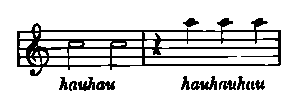
\includegraphics{hauhau.eps}
\end{center}

\noindent = der Hund bellt. Ähnliches beobachten wir wohl bei den Sprechversuchen der Kinder. \sed{Der Sprachlaut aber, selbst der onomatopoetische, muss sich den Fesseln der Schallmimik entrungen haben, um wahrer Sprachlaut zu werden; er muss abstrahiren, generalisiren, denn alle Sprache, selbst die roheste, bewegt sich in Abstractionen und nennt das Einzelne mit dem Namen der Gattung.}

Wir dürfen annehmen, dass unsere Altvordern ihre Rede mit lebhaftem Gesten- und Mienenspiel begleitet, oft auch durch solche optische Mittel ersetzt \sed{{\textbar}{\textbar}312{\textbar}{\textbar}}\phantomsection\label{sp.312} oder ergänzt haben. Was führte sie nun dazu, die Stimm- und Gehörsorgane vorzugsweise und am Ende fast ausschliesslich mit dem Geschäfte der Verständigung zu betrauen?

Vor Allem wohl die Natur der Objecte selbst. Solche sind in erster Reihe die Empfindungen des Menschen, deren Ausbruch zugleich, wenn auch ungewollt, eine Aufforderung an die Mitmenschen enthält. Freude, Angst, körperlicher oder seelischer Schmerz, Schreck, Erstaunen: sie alle drängen unmittelbar zu Stimmäusserungen.

Zweitens erregt Nichts in der Aussenwelt so sehr die Aufmerksamkeit des Menschen, wie der unerwartet in’s Gehör fallende Ton und die heftige Bewegung, die auch hörbar zu sein pflegt. Nun ist der Zustand des wachen Menschen der, dass er fortwährend etwas sieht, oft aber gar nichts hört, sei es, dass innerhalb seines Gehörkreises kein Schall ertönt, sei es, dass er der leisen und \fed{der} gewohnten Geräusche, wie etwa des Summens kleiner Insecten, nicht Acht hat. Darum ist der \update{Gehörsinn}{Gehörssinn} \fed{{\textbar}303{\textbar}}\phantomsection\label{fp.303} viel mehr den heftigen Überraschungen ausgesetzt, als der Gesichtssinn, darum führt er viel öfter dem Gemüthe heftige Erregungen zu. So ist der Zuruf das beste Mittel, um die Aufmerksamkeit der Mitmenschen auf uns zu ziehen, und er ist auch da wirksam, wo uns die Blicke Anderer nicht erreichen können. Dazu kommt, dass Gesichtseindrücke gleichzeitig vielerlei, Gehörseindrücke dagegen fast immer nur Eins auf einmal zu enthalten pflegen; man sieht viele Dinge zugleich, nimmt aber in der Regel auf einmal nur einen Schall deutlich wahr. Und jeder einzelne Gegenstand zeigt eine Mehrzahl optischer Eigenschaften: Grösse, Gestalt, Farbe, Ruhe oder Bewegung irgend welcher Art, – während unter seinen möglichen akustischen Wirkungen immer nur eine besonders sinnfällig und bezeichnend sein wird.

Drittens kann der Mensch mit seinen körperlichen Mitteln die Geräusche und Töne der Aussenwelt leichter und verständlicher nachahmen, als ihre Gestalten oder gar ihre Farben. Wo freilich die akustischen Vorstellungen fehlen, da musste mit optischen Mitteln nachgeholfen werden, und dieser Zwitterzustand der Sprache wird sehr lange angedauert haben. Wir werden bald weiter verfolgen, wie er doch am Ende durch allerlei Übertragungen überwunden werden konnte. \sed{Wir dürfen aber schon jetzt von \so{symbolisirender Onomatopöie} reden. Das Thier wird mit dem Tone, den es hervorzubringen pflegt, benannt, auch wenn es schweigt. Das Brechen, Fallen, Rollen, Schneiden, Reissen u. s. w. kann mehr oder minder geräuschlos geschehen; jenes Geräusch aber, von dem es andere Male begleitet war, bleibt nun sein conventionelles Zeichen. Aber noch mehr: Das Gemüth wird von verschiedenen Gehörsempfindungen sehr verschieden erregt, – recht eigentlich gestimmt; der Körper hat, je nach der Art, wie er berührt wird, sehr verschiedene Empfindungen, die wieder in ganz bestimmter Weise auf das Gemüth wirken, und auch diese Berührungen, das Schlagen,} {\textbar}{\textbar}313{\textbar}{\textbar}\phantomsection\label{sp.313} \sed{Schütteln, Stossen, Stechen, Streicheln u. s. w., können hörbar oder unhörbar geschehen. Nun arbeitet die Sprache in Analogien: das Stumme macht sie tönend, und das Körperliche überträgt sie auf’s Gemüthliche. Sie ist eine geschickte Bildnerin und schafft in geschmeidigem Stoffe.}

\sed{Vielleicht hat auch \textsc{B. Bourdon }\corr{1901}{(L’expression}{(d’expression} des émotions et des tendences dans le langage, Paris 1892 p. 38 flg.) Recht, wenn er auf das feine Taktgefühl der Zunge hinweist und vermuthet, die Zunge bewege sich so, dass sie selbst etwas Ähnliches empfinde, wie sie mit ihren Lauten ausdrücken wolle, sie schaffe sich selbst das Gefühl des Druckes, des Gleitens, Streichelns, Kitzelns u. s. w. und erzeuge dabei entsprechende Schallwirkungen. Der Hörer brauchte dann das Gehörte nur nachzuahmen, um an der eigenen Zunge Gleiches zu empfinden. Hier wäre also die Spracherzeugung auch imitativ, aber die Nachbildung gelte dem Tastsinne, die Schallwirkung wäre nur ein begleitender Nebenumstand. Die Hypothese ist gewiss feinsinnig; schon \corr{1901}{\textsc{Byrne}}{\textsc{Byren}} hatte eine ähnliche aufgestellt; mir scheint sie mehr glänzend als einleuchtend.}

Genug, schon jetzt haben wir vom Standpunkte des strenggläubigen Darwinismus aus ein recht buntes, wenn auch nicht gerade ein liebliches Bild vom Seelen- und Sprachleben unserer Altvordern gewonnen. Und seltsam, das Beste dabei musste sehr trüben Quellen entfliessen: Neid, Langeweile, Spieltrieb, Lüge, Eitelkeit, Neugier, Geschwätzigkeit, Alles musste mitwirken, um den sprechenden Menschen zu bilden. Wohl jede seiner Eigenschaften finden wir auch bei Thieren wieder, nirgends sonst aber, die guten inbegriffen, sie alle so beisammen. Vielseitigkeit der körperlichen und seelischen Beanlagung, ihr entsprechend wechselvolle \update{Mannich\-faltigkeit}{Mannig\-faltigkeit} der Schicksale und Beschäftigungen, stets zunehmende Menge der leiblichen und geistigen Bedürfnisse: das war es, was den Menschen zum Denker und Sprecher machte. Denn Beides, Denk- und Sprachvermögen, musste hinfort, sich wechselseitig fördernd, aneinander emporranken.

\pdfbookmark[2]{§4. Laute und Töne in der Ursprache.}{IV.II.4}
\cohead{§4. Laute und Töne in der Ursprache.}
\subsection*{§. 4.}\phantomsection\label{IV.II.4}
\subsection*{Laute und Töne in der Ursprache.}

Der Gedanke liegt nahe, es müsse die Phonetik der ältesten menschlichen Sprache besonders einfach gewesen sein: wenige Vocale, – man \fed{{\textbar}304{\textbar}}\phantomsection\label{fp.304} hat wohl an die drei angeblichen Urvocale \textit{a}, \textit{i}, \textit{u} gedacht, – und sehr wenige Consonanten, etwa dieselben, die wir zuerst von kleinen Kindern hören. Ich kann dies nicht glauben; dies eine Mal scheint mir der Rückschluss von der Kindersprache auf die Ursprache verfrüht.

Der Urmensch, wenn anders das Bild, das wir vorhin von ihm zu gewinnen suchten, zutrifft, schuf nicht nur eigene Laute, sondern lauschte auch der Aussenwelt ihre Schallwirkungen ab und übte sich diese nachzuahmen. So ward die \sed{{\textbar}{\textbar}314{\textbar}{\textbar}}\phantomsection\label{sp.314} ganze Natur seine Sprachlehrerin, und sein Sprach- und Stimmorgan sehr \update{mannich\-faltig}{mannig\-faltig} gebildet. Die Zwischenstufen der Vocale, die \textit{ä}, \textit{e}, \textit{o}, \textit{ö}, \textit{ü} u.~s.~w., wurden ihm \update{geläufig;}{geläufig,} \sed{– insofern sind sie jedenfalls ebenso ursprünglich, wie die drei „Urvocale“ \textit{a}, \textit{i}, \textit{u};} das Rauschen, Zischen, Spritzen und Summen, das um ihn her ertönte, lehrte ihn die \textit{š}, \textit{s}, \textit{ž}, \textit{z} anwenden; in krachenden, rollenden und rieselnden Geräuschen sprach ihm die Natur verschiedenerlei \textit{r} und \textit{l} vor; und galt es, den Knall einer berstenden Nuss, das Schnalzen und Zirpen verschiedener Thiere nachzubilden, so musste er sich mit jenen Schnalzlauten behelfen, die noch heute in südafrikanischen Sprachen erklingen. Auch seine Singstimme hatte, jetzt brüllend, brummend oder heulend, jetzt kreischend oder näselnd, jetzt wohl auch in reineren Tönen mitzuwirken.

Ausdrucksvoll war die Intensität der Hervorbringung, bald für die innere Stimmung, bald für die Stärke des äusseren Geschehens, die freilich wieder stimmend wirkte. Noch mochten die Tenues und Mediae, vielleicht sammt ihren Aspiraten, nur Gradverschiedenheiten ausdrücken, sonst frei untereinander vertauscht werden, wie noch heute in manchen Sprachen.

Dass die Ursprache durchgängig und ausschliesslich aus \update{Einsylblern}{Einsylbern} bestanden habe, ist nicht glaublich. Schon das Kind gefällt sich in Doppelungen, und die Aussenwelt, zumal die Thierwelt, giebt uns deren in Menge zu hören. Aber auch zu Verbindungen verschiedenlautiger Sylben bot die Natur dem Menschen Vorbilder, so im Knattern und Dröhnen eines nahen Donners oder eines stürzenden Baumes und in den Rufen mancher Vögel. Andrerseits konnten auch manchmal vocallose Explosivlaute der Darstellung besser dienen, als volle Sylben. Brennendes Holz z.~B. lässt oft ein deutliches \textit{b’} vernehmen; \textit{t’} und \textit{pf’}, \textit{ph’} sind Laute des Spuckens und heftigen, blasenden Ausathmens. Wenn man an die verwandten Demonstrativlaute der meisten Sprachen denkt, so gewinnt man von den Manieren unserer Altvordern kein sonderlich anmuthiges Bild.

\fed{{\textbar}305{\textbar}}\phantomsection\label{fp.305}

Der Fortschritt aber, den das Lautwesen im Laufe der Zeit zu machen hatte, wird weniger in der Einführung und Unterscheidung neuer akustischer Mittel, als in der Ausscheidung mancher der vorhandenen bestanden haben, in einer Art natürlicher Zuchtwahl. Die gebräuchlichsten, darum bequemsten vertraten die selteneren, verdrängten sie allmählich. Mir ist leider hiefür kein besseres Beispiel zur Hand, als jenes {\ain}\textit{a}{\ain}\textit{a} der kleinen Kinder, das bedeutsam krächzend mit zwei entschiedenen {\ain}\textit{Ain} gesprochen wird. Diesen Laut haben manche Sprachen in überraschender Einhelligkeit durch das ihnen geläufigere \textit{k} \update{ersetzt.}{ersetzt,} \sed{so z. B. viele indogermanische, das Mandschu, das Syrjänische, das Tibetische, das Quechua, das Odschibwe.} Das stilisirte Lautzeichen trat an Stelle des getreuen Abbildes, ganz wie das optische Zeichen in der hieratischen Schrift gegenüber der hieroglyphischen Malerei; die Sprache entrang sich der Sklaverei ihrer Vorbilder, und eben hierin lag eine That wahrhaft menschlichen Fortschrittes. 

\sed{{\textbar}{\textbar}315{\textbar}{\textbar}}\phantomsection\label{sp.315}

Absichtlich habe ich mich auch diesmal wieder mit der flüchtigen Andeutung von Wahrscheinlichkeiten begnügt. Dichten, phantasiren kann man ja in’s Endlose. Eine leidlich erschöpfende, inductive Erforschung der Naturlaute in der Ursprache, wenn sie überhaupt je möglich werden sollte, würde genealogisch-historische Arbeiten voraussetzen, von deren Ergebnissen wir Jetztlebenden uns keine Vorstellung machen können.

\pdfbookmark[2]{§5. Die Personificirung, Beseelung und Belebung.}{IV.II.5}
\cohead{§5. Die Personificirung, Beseelung und Belebung.}
\subsection*{§. 5.}\phantomsection\label{IV.II.5}
\subsection*{Die Personificirung, Beseelung und Belebung.}

\largerpage[1]Der Mensch erkennt im Mitmenschen Seinesgleichen, beurtheilt ihn nach sich und urtheilt damit in der Regel richtig. Im Thiere erkennt er ein ihm ähnliches Wesen, sucht und findet in ihm dieselben Bedürfnisse und Leidenschaften, auch annähernd dieselben Kräfte, die ihn selbst bewegen. Auch dieselben geistigen Kräfte; darum mag Kinder und kindliche Völker die Thierfabel ganz anders anmuthen, als uns. Aber auch mit dem Pflanzenreiche und mit der ganzen Welt des Unorganischen weiss sich der Mensch bald in freundlichem bald in feindlichem Verkehre. Ob ihn ein Dorn ritzt, eine Katze krällt, oder ob ihn ein Mitmensch seine Nägel fühlen lässt: seine Empfindung ist die gleiche, – warum sollten Jene, die ihm den Schmerz verursacht, nicht auch das Gleiche beabsichtigt haben? warum sollte er dem Einen mehr zürnen, \fed{{\textbar}306{\textbar}}\phantomsection\label{fp.306} als dem Anderen? Das Kind, das sich gegen die Tischkante stösst, prügelt den Tisch: „Wart’, du böser Tisch!“ Der Tisch wird ihm ein Du, eine zweite Person, die also auch ihr Ich haben wird, ein böses, feindliches Ich. Ein liebes Spielzeug aber küsst es, und wenn es recht blank geputzt ist, freut sich das Kind gleich mit in die Seele der Sache hinein, denn es hat eben die Sache beseelt. Auch uns Erwachsenen und Gebildeten kann es, wenn wir nicht froschkühl sind, in unbewachten Momenten ähnlich ergehen. Dann lassen wir an Sachen, die uns ärgern, unsern Ärger aus, zerknicken die Feder, die nicht schreiben will, oder rufen ihr eine Verbalinjurie nach, während wir sie wegwerfen. Der Zorn thut dabei die Hauptsache; denn dem Widerspenstigen legen wir eher einen eigenen Willen unter, als dem \update{Gefügigen.}{gefügigen.} Bei rohen Völkern thut aber auch die Furcht ihr Theil. Was mir schaden kann, das kann ich vielleicht durch Bitten und Wohlthaten versöhnen, sodass es nicht mehr mir, sondern meinen Feinden, schadet, mir ein Bundesgenosse, ein Schutzgott (Fetisch) wird. Und was mir nun dient und nützt, das ist mein Freund, mit dem stelle ich mich auf Du und Du. Dieser naiven Anschauung dünkt Alles erklärlich: Alles hat sein Ich, seinen Willen, – warum sollte dieser Wille weniger launenhaft sein, als der meinige? Sagen wir doch selbst von einer Uhr oder einer Flinte, die ohne erkennbaren Grund ihren Dienst versagen: sie haben ihre Mucken. \sed{Jene unpersönlichen Verba, die} {\textbar}{\textbar}316{\textbar}{\textbar}\phantomsection\label{sp.316} \sed{bei uns die Witterungsereignisse erzählen: „es regnet, es donnert“ u. s. w. sind nichts weniger als naiv. Das Kind will wissen, \so{wer} donnert? Und ob man ihm dann antwortet: „Der liebe Gott“ oder: „Der böse Mummum“, – so ist es für’s Erste befriedigt; ihm ist jedes Geschehniss eine That. Nun weiss es auch den Thäter, – was will es mehr? Verbinden sich nun That und Thäter unlösbar, wird jedem Naturereignisse sein besonderer Urheber zugetheilt, das Nomen actoris zum Nomen proprium \corr{1901}{erhoben:}{erhaben:} so ist das Personal für einen wohlbesetzten Olymp leicht zusammengebracht.}

Kein Zweifel, diese naive Beseelung der Welt hat an der Schöpfung und Ausgestaltung der menschlichen Sprache mächtig mitgewirkt. Für menschliches Thun und Empfinden waren die Benennungen da. Indem man die Dinge vermenschlichte, ergaben sich leicht die Ausdrücke für ihre Äusserungen und darnach die Namen für sie selbst. Hier fanden die Launen einer jugendlichen Phantasie ihren breitesten Spielplan. Jeder durfte thun, was heute nur den Dichtern vergönnt ist.

Wo immer wir der Herkunft der Ausdrücke, der lexikalischen oder der grammatischen, folgen können, es handle sich um klare Zusammensetzungen oder um syntaktische, periphrastische Gebilde, überall ist der Hergang der gleiche: es sind Übertragungen, das Seelenlose wird wie ein Beseeltes, das Leblose wie ein Belebtes behandelt, und des Protagoras Wort gilt auch hier: Der Mensch ist das Mass aller Dinge. Manchmal ist es, als feierte die durchgeisterte Welt der Urmenschen in den jüngsten Sprachen ihre Auferstehung. Der Franzose lässt den Stein „milden \fed{{\textbar}307{\textbar}}\phantomsection\label{fp.307} Sinnes“, doucement, dahinrollen; und wenn es nicht gelingt, einen Nagel in die Wand zu treiben, so sagt der Engländer: „It will not hold“, und der Obersachse sagt wohl: „Es lernt nicht halten“, als fehlte es dem Nagel am guten Willen oder gar an der nöthigen Intelligenz! \sed{Dazu kommt nun das ganze Heer der sonstigen Übertragungen:}

\sed{von Sinne zu Sinne, zumal zwischen Gesicht und Gehör, z. B. helle, dunkele, tiefe Töne in der Musik und in der Malerei,}

\sed{von einem Naturreiche oder Körper zum anderen, z.~B. malaisch \textit{māta hāri}, Auge des Tages = Sonne, \textit{māta āyer}, Auge des Wassers = Brunnen, \textit{ānaq pōhon}, Kind des Baumes = Strauch, \textit{ānaq māta}, Kind des Auges = Augapfel,}

\sed{von Körperlichem auf Geistiges: eiserne Stirn = Frechheit, feine Nase = Spürsinn. – Ähnliches und vielleicht noch Stärkeres darf man auch der Phantasie des Urmenschen zutrauen.}

Der Spielraum ist unendlich weit, der Wege sind unzählbar viele. Und doch sollte man meinen, auch was wie Laune und Willkür scheint, müsse seine Gesetze haben. Man kann ja Alles vergleichen, was irgend Ähnlichkeiten bietet. Aber nicht alle Vergleiche sind gleich gut, und unter den guten finden die gleichwerthigen nicht allemal gleichmässig Anklang. Die Ähnlichkeit muss sofort \sed{{\textbar}{\textbar}317{\textbar}{\textbar}}\phantomsection\label{sp.317} einleuchten: darin besteht die Güte des Vergleiches. Und das Vergleichsbild muss dem Kreise unseres gewöhnlichen Denkens entlehnt sein: darauf beruht sein Anspruch auf Volksthümlichkeit, das heisst auf dauernden Platz im Sprachgute. So müsste die Etymologie der Wörter und Wortformen von der Sinnes- und Lebensweise der alten Völker zeugen, – wenn sie nur etwas deutlicher reden wollte.

In der That würde sie dann noch von ganz anderen Dingen erzählen. Denn nicht nur das Mass, sondern auch der Mittelpunkt der Welt ist der Mensch, dünkt sich es zu sein. Alles dreht sich um ihn, bewegt sich nach ihm hin oder von ihm weg; was über ihm ist, ist oben, was hinter ihm liegt, ist hinten, und um ihn herum zieht sich der Kreis dessen, was er sein nennt und scharfen Blickes unterscheidet, – jenseits in immer weiteren, immer nebelhafteren Kreisen, das Andere, Fremde, das er, je ferner es ihm steht, um so unbestimmter erschaut und benennt. Die Anfänge der Mensehheitsgeschichte müssten sich in der Etymologie spiegeln, wenn es je gelänge, diesen Spiegel von den ihn überlagernden vieltausendjährigen Staubschichten zu säubern. Doch darauf kommt es für jetzt nicht an, nicht auf das Bild, das die Alten gemalt haben, sondern auf den Malkasten, dem sie ihre Farben entnahmen. Wie sie nun weiter die empfangenen Eindrücke von Sinne zu Sinne übertragen mochten, dafür liefern uns die heutigen Sprachen Beispiele die Hülle und Fülle.

\fed{{\textbar}308{\textbar}}\phantomsection\label{fp.308}

\pdfbookmark[1]{III. Capitel.}{IV.III.Capitel}
\cehead{{{\large IV,}} III. Inhalt und Form der Rede.}
\pdfbookmark[2]{I. Die Rede.}{IV.III.I}
\cohead{I. Die Rede.}
\section*{III. Capitel.}\phantomsection\label{IV.III}
\section*{Inhalt und Form der Rede.}
\subsection*{I.}\phantomsection\label{IV.III.I}
\subsection*{Die Rede.}
Sprache ist Rede, ist Ausdruck des Gedankens, ist Satz. Wir fragen zunächst nach dem Inhalte der Rede: Welcher Art Gedanke wird ausgedrückt, welcher Art ist also die Rede, der Satz?

Wir müssen hier wieder etwas weiter ausholen. Denken heisst Vorstellungen verknüpfen. Die Eintheilung der Vorstellungen in Anschauungen und Begriffe überlassen wir vorläufig der Philosophie. Die Rede ist Ausdruck jener Verknüpfung von Vorstellungen, also Ausdruck sowohl der zu verknüpfenden Vorstellungen, als auch ihrer Verknüpfung, mag diese Verknüpfung noch so lose, ihr Ausdruck noch so schwächlich sein.

Wollten wir hierbei stehen bleiben, von diesem Standpunkte aus die Arten der Rede zu classificiren versuchen, so wüsste ich keinen anderen Eintheilungs\-\sed{{\textbar}{\textbar}318{\textbar}{\textbar}}\phantomsection\label{sp.318}grund, als jene verschiedenen Verknüpfungsweisen: ob thatsächlich, möglich, nothwendig, gewiss, gewollt u.~s.~w. Dann würden also die Sätze:

~~~~Du kommst,

~~~~Du sollst kommen,

~~~~Du kannst kommen, 

~~~~Du musst kommen, 

~~~~Du kommst hoffentlich, 

~~~~Du kommst wahrscheinlich, 

\largerpage[-1]\noindent ebensoviele verschiedene Formen der Rede darstellen.

Offenbar \update{thuen}{thun} sie dies nicht; der Standpunkt, von dem aus wir die Eintheilung versuchten, war verfrüht. Worin lag nun der Fehler? Darin, dass wir nur an das redende Ich dachten, nicht auch an das angeredete Du. Ein solches ist entweder vorhanden oder nicht vorhanden. Nicht vorhanden ist es nur im Falle des eigentlichen Ausrufes. Sonst ist es überall, mindestens im Geiste des Redenden, gegenwärtig, die Rede ist im weiteren Sinne Gedankenmittheilung, mag ich nun den Angeredeten in ein Wir mit einschliessen, mag ich mir im Selbstgespräche mich selbst \fed{{\textbar}309{\textbar}}\phantomsection\label{fp.309} wie im Spiegelbilde gegenüberstellen. Wir wollen zunächst die mittheilende Rede in diesem weiteren Verstande in’s Auge fassen. Denn die folgenden Untersuchungen werden uns in ein wirres Gebiet führen, und es ist gut, da anzufangen, wo noch die Dinge am Klarsten zu liegen scheinen.

Nun enthält jede Rede unmittelbar eine Aufforderung an das Du: „Höre mich!“ Bekanntlich giebt man in manchen Gegenden und Sprachen dieser Aufforderung noch besonderen Aus- und Nachdruck. „Höre, – \textit{écoutez}.“

Verlange ich nichts weiter als Aufmerksamkeit, so ist meine Rede \so{Declamation} im weiteren Sinne des Wortes. Dann stelle ich mir aber unter dem Du jemand anderes vor, als meine Zuhörerschaft, und an dies Du stelle ich noch andere Anforderungen. Wende ich mich aber an die Zuhörerschaft, wird die Declamation zur Ansprache, so stehen wir wieder auf dem alten Punkte: ich verlange von den Angeredeten noch etwas mehr als blosse Aufmerksamkeit. Um dieses Mehrere wird es sich hier handeln.

\phantomsection\label{IV.III.I.1}1. Ich spreche meinen Gedanken aus und verlange, dass der Angeredete nun ebenso denke: „Glaube mir!“ Die entsprechende Form der Rede ist die \so{mit\-thei\-lende im engeren Sinne}: ich theile Dir meinen Gedanken mit, damit er hinfort auch Dein Gedanke werde.

\phantomsection\label{IV.III.I.2}2. Ich kann Dir nichts mittheilen, was ich nicht habe oder zu haben vorgebe. Du kannst mir nichts glauben, was ich nicht – mindestens vorgeblich – glaube oder weiss. Bin ich aber selbst im Ungewissen, so kannst Du vielleicht mir mit\-theilen, was mir fehlt. Nun begehre ich dies von Dir: „Sage \sed{{\textbar}{\textbar}319{\textbar}{\textbar}}\phantomsection\label{sp.319} mir...!“ Die dem entsprechende Redeform ist die \so{fragende}. Die antwortende dagegen ist ihrer Natur nach nur eine Unterart der mittheilenden.

\phantomsection\label{IV.III.I.3}3. Ich will weder, dass Du etwas durch mich erfahrest, noch dass ich etwas durch Dich erfahre, sondern dass Du etwas, gleichviel was, thuest oder unterlassest Die Form dieser Rede nennen wir die \so{gebietende} (verbietende, bittende, verbittende).

\phantomsection\label{IV.III.I.4}4. Die menschliche Sprache ist ihrem Wesen nach Verkehrsmittel; dass dem Redenden ein Du mindestens im Geiste gegenwärtig sei, bildet die Regel. Allein ebenso ist es die Regel, dass ich nicht nur Dir etwas sagen, sondern auch mich aussprechen will; ich will selbst hören, was ich denke, und wie ich empfinde. In solchen Stimmungen befindet sich \fed{{\textbar}310{\textbar}}\phantomsection\label{fp.310} der Mensch unter dem Einflusse mächtiger Erregungen, die nach Entladung drängen. Was er zu dem Ende thut, ist im weiteren Sinne pathologisch, es sei Weinen, Lachen, Händeklatschen, Aufstampfen mit dem Fusse, ein Aufschrei, ein Schnalzen mit der Zunge oder ein Stück menschlicher Rede. Denn auch die Sprache ist uns durch Übung so zur Natur geworden, dass sie unbewusst und absichtslos aus unserm Innern hervorbrechen kann. Solche Reden nun nennen wir \so{ausrufende}. Wir mussten ihrer besonders gedenken, zunächst weil sie in der That auf anderer seelischer Grundlage beruhen, als jene, welche dem Verkehre dienen; dann aber auch, weil es nahe liegt, dass sich die Sprache, wo sie die Fesseln des Verkehres abgestreift, neue Formen geschaffen habe.

\label{IV.III.I.5}Jetzt gilt es, die gewonnene Eintheilung auf ihre Durchschlägigkeit und Vollständigkeit zu prüfen, und da erstehen auf den ersten Blick ernstliche Bedenken, die beseitigt werden müssen.

A. Wir haben uns an die herkömmlichen Benennungen gehalten, der mittheilenden Rede die fragende und die befehlende entgegengesetzt, die doch in Wahrheit auch einen Gedanken des Redenden mittheilen sollen.

B. Wir haben die fragende Rede der befehlenden nebengeordnet. Der Befehl verlangt vom Angeredeten eine positive oder negative Thatäusserung: Thue das, unterlasse jenes! Eine solche Thatäusserung ist aber doch auch die Antwort, zu der der Gefragte aufgefordert wird. Also könnte es scheinen, als wäre die Frage nur eine Unterart des Befehles.

\largerpage[1]C. Endlich kleidet die Sprache oft ihre Gedanken in geborgte Gewänder. Die \so{mittheilende} Redeform mag jetzt eine Frage enthalten: „Ich wüsste gern ob ...“, – jetzt mag sie einen Befehl, eine Bitte, ein Verbot in sich schliessen: „Du musst ..., Du darfst nicht ..., Du würdest mir einen Gefallen \update{thuen,}{thun,} wenn Du ...“ u.~s.~w. Die fragende Form mag ein fertiges Urtheil verhüllen. Es ist dies der Fall der rhetorischen Frage, die besagen will: „Gieb die Antwort nicht mir, sondern Dir, stelle Dir die Frage, so wirst Du urtheilen wie ich!“ Oder es mag eine Aufforderung in fragender Form ausgesprochen werden. „Wirst \sed{{\textbar}{\textbar}320{\textbar}{\textbar}}\phantomsection\label{sp.320} Du gleich kommen?! Wärest Du wohl so freundlich ...?“ Es scheint naturgemäss, dass auch der Ausruf gern die fragende Form annehme: „Wie schön ist das!“ Denn der Zustand der Gemüthserregung ist jenem des unfertigen Urtheils verwandt. Die \so{befehlende} und \so{bittende} Form eignet sich ohne Weiteres da, wo Auskunft erfordert wird: \fed{{\textbar}311{\textbar}}\phantomsection\label{fp.311} „Nenne mir Deine \update{Gehülfen!}{Gehilfen!} Sagen Sie mir doch die genaue Zeit!“ Endlich kann der Ausruf jetzt eine thatsächliche Mittheilung bezwecken: „Ein schönes Bild!“, – jetzt eine Frage: „Wüsste ich doch ...!“ – jetzt wohl auch eine Aufforderung: „Wenn Du mir doch hülfest!“ 

Wir halten uns an die Formen und stellen nun der ausrufenden die drei übrigen als mittheilende im weiteren Sinne gegenüber.

Der mitzutheilende Gedanke kann sein ein Urtheil, ein Wunsch, oder \update{beides}{Beides} zugleich.

Er sei ein Urtheil, so kann dieses vollständig oder unvollständig sein. Ist es vollständig, so ist die Rede \so{mittheilend im engeren Sinne des Wortes}.

Ist das Urtheil unvollständig, so theile ich es dir als unvollständiges mit, um es von dir ergänzen zu lassen. Beides, jene Mittheilung eines Urtheils und jener ausgesprochene Wunsch nach dessen Vervollständigung, vereinigt sich in der \so{Frage}.

Endlich: der Gedanke sei vollständig, aber er sei nicht ein Urtheil, sondern ein Wunsch, dessen Erfüllung ich von dir begehre: so sind die Voraussetzungen gegeben zur \so{befehlenden} Rede und ihren Verwandten: der bittenden, \update{verbittenden,}{verbietenden,} rathenden u.~s.~w.

Zur Übersicht stellen wir für die drei mittheilenden Redeformen folgendes Schema auf:

\begin{table}[h]
\centering
\begin{tabular}{c c c c c c}
& \multicolumn{3}{c}{Der mitzutheilende Gedanke ist} \\
\multicolumn{1}{l}{\hspace*{.7cm}\tikzmark{urteil}{ }} & & & &
\multicolumn{1}{r}{\tikzmark{wunsch}{ }\hspace*{1cm}} & \\
\multicolumn{2}{c}{A. ein Urtheil. Dies ist} & & \multicolumn{2}{c}{B. ein Wunsch} \\
\multicolumn{1}{l}{\tikzmark{vollstaendig}{ }} & \multicolumn{1}{r}{\tikzmark{unvollstaendig}{ }} & & \multicolumn{2}{l}{\pushbar} \\
\multicolumn{1}{l}{a) vollständig} & \multicolumn{1}{r}{b) unvollständig} & & \multicolumn{2}{l}{\pushbar} \\
\LARGE {\textbar} & \multicolumn{2}{c}{ \LARGE {\textbar} } & \multicolumn{2}{l}{\pushbar} \\
\LARGE {\textbar} & \multicolumn{2}{l}{\tikzmark{frage}{ }} & \multicolumn{2}{r}{\tikzmark{befehl}{ }} \\
\multicolumn{1}{l}{1. Mittheilung} & \multicolumn{2}{c}{2. Frage} & & \multicolumn{1}{r}{3. Befehl u.~s.~w.}
\end{tabular}
\end{table}

\tikz[overlay,remember picture] {

\draw[style={decorate,decoration={brace}}, thick] (urteil) -- (wunsch) node {};

\draw[style={decorate,decoration={brace}}, thick] (vollstaendig) -- (unvollstaendig) node {};

\draw[style={decorate,decoration={brace,aspect=0.62}}, thick] (frage) -- (befehl) node {};
}

Ich glaube, diese Tabelle trägt die Gewähr der Vollständigkeit in sich, und sie wird noch ein zweites Mal analog anwendbar sein, wenn es gilt, die \so{ausrufende} Rede in Unterarten zu theilen.

Unterscheiden wir auch hier wieder zwischen Inhalt und Form.

Der Form nach kann der Ausruf sein:

\phantomsection\label{IV.III.I.A}A. ein vollständiger Satz \update{bez.}{bezw.} ein Satzwort, z. B. ein optativer: „Käme er doch!“ oder ein fragender. „Wie schön ist das!“ Ein Imperativ: „Halt!“ An die besonderen modalen Verbalformen oder \update{Hülfswörter,}{Hilfswörter,} die in manchen Sprachen der ausrufenden Rede \retro{dienen,}{dienen;} mag hier nur im Vorübergehen erinnert werden.

\fed{{\textbar}312{\textbar}}\phantomsection\label{fp.312} \sed{{\textbar}{\textbar}321{\textbar}{\textbar}}\phantomsection\label{sp.321}

\phantomsection\label{IV.III.I.B}B. Elliptisch, einen Satz ersetzend, z. B. „Brav gemacht!“ „Abgeblitzt!“ „Schon wieder Einer!“ Manchmal werden wohl solche Ellipsen durch einen nachträglichen Zusatz ergänzt zu vollständigen Sätzen, und dann mag sich der seelische Hergang in einer eigenartigen Anordnung der Satzglieder ausprägen: „Schon wieder Einer – kommt da an!“ „Ein wunderlicher Mensch, – ist NN.“ So finden wir im Chinesischen: \textit{šén tsāi!} Gut, traun! Aber auch, mit nachträglicher Nennung des Subjectes: \textit{šén tsāi wén}, gut, traun, (war deine) Frage! Wir reden dann von Inversionen, müssen aber bedenken, dass diese nicht, wie rechtschaffene Sätze, in der Seele fertig vorher geformt waren, sondern erst hinterdrein, so zu sagen durch einen späteren Anbau, zu einem Ganzen geworden sind. – Die beiden bisherigen Formen sind wohl ausrufend und werden auch von den Zuhörern so aufgefasst. In der That pflegen aber solche Ausrufe nur dann über unsere Lippen zu kommen, wenn wir wissen, dass man uns hört, und wollen, dass man uns höre. So könnte es scheinen, als wären sie doch im weiteren Sinne mittheilend. Ich denke indessen daran, wie oft uns derlei Ausrufe auf den Lippen schweben und ungeäussert bleiben, unterdrückt werden. Warum das? Weil es doch zu nichts frommen würde, sie verlauten zu lassen. Sprechen wir sie Dritten gegenüber aus, so ist der Thatbestand dieser: Wir bezwecken eine Mittheilung, machen diese aber in solcher Form, als sprächen wir lediglich mit der Absicht, unserer übervollen Seele ein Ventil zu öffnen. Man sagt wohl: „Es musste heraus, ich musste mich aussprechen“, und dann empfindet man es als eine doppelte Erleichterung, wenn nun Andere in Mitleidenschaft gezogen werden. – Imperative wie: „Hut ab!“ „Still gestanden!“ sind Zurufe, also Mittheilungen im weiteren Sinne des Wortes, nicht Ausrufe.

\largerpage[-2]\phantomsection\label{IV.III.I.C}C. Vocative im weiteren Verstande des Wortes, ich möchte sagen in zweiter und dritter Person, sind absolute, der Satzverknüpfung entbehrende substantivische Redetheile, die sich aber nicht an eine vorhandene oder vorgestellte zweite Person richten. Dahin gehören in vielen Fällen die Anrufungen übersinnlicher Mächte oder fürchterlicher Ereignisse, z.~B. „Herr Gott!“ „Den Teufel!“ „Donnerwetter!“ „Schwere \update{Noth.“}{Noth“.} Es sind das Stimmungsäusserungen, mit denen keinerlei Gebet oder Beschwörung beabsichtigt wird: man denkt an gar keine zweite Person. Auch pflegt man bei solchen Ausrufen nicht an etwaige Zuhörer zu denken. Das unterscheidet sie von jenen Vocativen und sonstigen \fed{{\textbar}313{\textbar}}\phantomsection\label{fp.313} Zurufen, die an ein Du gerichtet sind: Polizei! Hülfe! Feuer! Diese sind im weiteren Sinne mittheilend. – Ob der interjectionelle Accusativ im Lateinischen, z. B. \fed{Me} miserum! hierher oder unter die Ellipsen gehört, wage ich nicht zu \update{entscheiden.}{unterscheiden.}

\phantomsection\label{IV.III.I.D}D. Reine Interjectionen, das heisst Wörter, die keinem anderen Redetheile angehören. Sie dürften einzutheilen sein

\phantomsection\label{IV.III.I.a}a) in mehr objective, nachahmende, z.~B. Pardauz! hopsa! puff!

\phantomsection\label{IV.III.I.b}b) in mehr subjective, d.~h. solche, die nur ein individuelles Empfinden, \sed{{\textbar}{\textbar}322{\textbar}{\textbar}}\phantomsection\label{sp.322} Schmerz, Freude, Erstaunen u.~dgl. ausdrücken: Au! Ei! Ach! Hm! Es sind dies ungeformte Wörter, die der geformten Sprache gegenüber auch in lautlicher Hinsicht eine Ausnahmestellung einnehmen können. In ihnen hat das Hochdeutsche noch anlautende \textit{p}, haben Dialekte, die sonst \textit{ö} und \textit{ü} in \textit{e} und \textit{i} verwandeln, diese Laute rein bewahrt. In beiden Hinsichten stehen ihnen gewisse Auf- und Zurufwörter gleich, z.~B. das Hö und Hüist der Fuhrleute und Ackerknechte in Sachsen, das Ruhe gebietende St! Auch das fragende Hm? ist hierher zu rechnen, und gewiss ursprünglich auch die Deutelaute, die den Demonstrativpronominibus zu Grunde liegen mögen. Solche „Naturlaute“, wie man sie wohl genannt hat, mögen zuweilen verstümmelte oder unverstandene ältere organische Gebilde in sich enthalten. Unser Jemine! ist wohl ein Ersatz für den Namen Jesus, vielleicht mit Anklang an \textit{domine}. In Spanien ruft man arglos: \textit{Caramba!} statt des unfläthigen \textit{carajo}, wie man in manchen Gegenden Deutschlands Gottstrambach oder ’strambach statt Gott straf’ mich sagt. Umgekehrt können jene Laute als Wurzeln oder Stämme grammatische Formung erfahren. Man sagt: die Katze miaut (maunzt), le chat miaule. Von ach! und pfui! bilden wir \retro{ächzen}{ächsen} und (mundartlich) pfuzen, ganz wie duzen und siezen von Du und Sie. Dass Thiere nach ihren Rufen benannt werden, ist wohl allgemein verbreitet. Der Kukuk hat selbst dafür gesorgt, dass die germanische Lautverschiebung seinem Namen nichts anhaben konnte. Von jenen Onomatopöien aber, die in die Urgeschichte der Sprache fallen, brauchen wir hier nicht wieder zu reden. 

\largerpage[-2]\phantomsection\label{IV.III.I.6}Mit Obigem sind meines Wissens die möglichen Formen der ausrufenden Rede erschöpft. In der That die möglichen Formen der menschlichen Rede überhaupt. Diese ist entweder grammatisch geformt oder ungeformt. Die geformte ist entweder ein vollständiger Satz oder kein vollständiger Satz. Letzteren Falles ist sie entweder ein zur Ergänzung aufforderndes Bruchstück eines Satzes – elliptisch, – oder sie lehnt \fed{{\textbar}314{\textbar}}\phantomsection\label{fp.314} die syntaktische Verknüpfung formell ab, ist absolut. Die vierte Kategorie, jene der ungeformten Sprachäusserungen, theilten wir so, dass die Eintheilung zugleich den Ursprung und den Inhalt betraf. Soll sie nun auch auf die mittheilenden Sprachäusserungen bezogen werden, so gerathen wir in Schwierigkeiten, die wir besser noch vermeiden. Wir fassen aber das bisher Gewonnene in ein Schema zusammen.

\begin{table}[h]
\centering
\tabcolsep=0.5cm
\begin{tabular}{l r l}
\multicolumn{3}{c}{Der sprachliche Ausdruck ist} \\
\tikzmark{geformt}{ } & & \multicolumn{1}{r}{\tikzmark{ungeformt}{ }\hspace*{1cm}} \\
\multicolumn{1}{c}{A. grammatisch geformt} & & \multicolumn{1}{c}{B. ungeformt} \\
\tikzmark{vollersatz}{ } & \tikzmark{absolut}{ } & \multicolumn{1}{c}{\LARGE {\textbar}} \\
\multicolumn{2}{c}{a) voller Satz, b) Ellipse, c) absolut,} & a) nachahmend, \\
& & b) Empfindungen äussernd, \\
& & c) deutend, \\
& & d) fragend . . .
\end{tabular}
\end{table}

\tikz[overlay,remember picture] {

\draw[style={decorate,decoration={brace}}, thick] (geformt) -- (ungeformt) node {};

\draw[style={decorate,decoration={brace}}, thick] (vollersatz) -- (absolut) node {};
}

\sed{{\textbar}{\textbar}323{\textbar}{\textbar}}\phantomsection\label{sp.323}

\noindent Nun aber, da wir die im weiteren Sinne mittheilende Rede mit in Betracht ziehen, müssen wir auch den Begriff der Ellipse ausdehnen auf jederlei eigentliches Satzfragment, auch auf den Fall, wo im Zwiegespräche die Ergänzung zum Satze aus der Rede des Anderen zu erholen ist, \retro{z.~B.}{z.~B,} Wer war dort? – Ich (war dort). – Wann (warst Du dort)? – Gestern. – Nun? Und ... ? (was geschah da?)

Jetzt kehren wir zur ausrufenden Rede zurück, um ihren möglichen Inhalt zu untersuchen.

Im Ausrufe äussert sich eine lebhafte Erregung, entweder nur die Art dieser Erregung, oder auch ihr Grund. Der Grund kann sein ein Wunsch oder eine vollendete Thatsache. Ist er eine solche, so kann die Erregung entweder in dem bekannten Theile der Thatsache, oder darin beruhen, dass wir einen Theil der Thatsache nicht kennen. Das Schema, das wieder den Eindruck der Vollständigkeit machen würde, gestaltet sich demnach folgendermassen :

\begin{table}
\begin{tabular}{c r r r}
\multicolumn{3}{c}{Äusserung der Erregung, und zwar} \\
\multicolumn{1}{l}{\tikzmark{art}{ }} & & \multicolumn{1}{r}{\tikzmark{grund}} \\
\multicolumn{1}{l}{A. nur ihrer Art nach,} & \multicolumn{2}{c}{B. auch ihrem Grunde nach} \\
 & \multicolumn{1}{l}{\tikzmark{wunsch}{ }} & \multicolumn{1}{r}{\tikzmark{tatsache}{ }} \\
 & \multicolumn{1}{r}{a) Wunsch,} & \multicolumn{1}{r}{b) Thatsache,} \\
 & \multicolumn{1}{r}{\tikzmark{alpha}{ }} & & \multicolumn{1}{r}{\tikzmark{beta}{ }} \\
 & & \multicolumn{2}{l}{α) Bekanntes, β) Unbekanntes.}
\end{tabular}
\end{table}

\tikz[overlay,remember picture] {

\draw[style={decorate,decoration={brace}}, thick] (art) -- (grund) node {};

\draw[style={decorate,decoration={brace}}, thick] (wunsch) -- (tatsache) node {};

\draw[style={decorate,decoration={brace}}, thick] (alpha) -- (beta) node {};
}


Setzen wir hier Thatsache und Urtheil auf eine Stufe, so ist die Analogie mit dem ersten Schema einleuchtend: Es laufen parallel: 

\ I. Wunsch – Befehl u.~s.~w.

II. Thatsache – Urtheil. 

\fed{{\textbar}315{\textbar}}\phantomsection\label{fp.315}

\ \ a) Bekanntes – Mittheilung. 

\ \ b) Unbekanntes – Frage.

Mag ich nun meine Erfahrungen mustern, mag ich versuchen, der Sache auf apriorischem Wege beizukommen, so finde ich weder die Möglichkeit zu einem neuen Schema noch zu einer Ergänzung in einem der vorhandenen Schemata, ich finde weder einen weiteren Eintheilungsgrund, noch eine Lücke in den gemachten Eintheilungen. Täusche ich mich hierin nicht, so wäre also die logische Aufgabe gelöst, und nun könnte es scheinen, als wäre ein Mittel gefunden, um jederlei Rede mit Leichtigkeit zu classificiren.

So einfach liegen indessen die Dinge nicht. Wir befinden uns nicht auf dem glattgefegten Boden der Logik, sondern mitten drinnen in dem üppigen Gewirre psychologischer Möglichkeiten. Da sind wie in einem Urwalde die Wurzeln und Gezweige der verschiedensten Pflanzen ineinander verfitzt, und Schlinggewächse ranken von Stamme zu Stamme. Jene dendrologischen Gärten aber, wo die Pflanzen säuberlich nach Arten und Unterarten in Beete und Reihen geordnet sind, sind recht eigentlich die Stätten, wo man den Wald vor lauter \sed{{\textbar}{\textbar}324{\textbar}{\textbar}}\phantomsection\label{sp.324} Bäumen nicht sieht. Und die Menschenseele schaltet schrankenloser als die schaffende Natur; vor keiner Zwitterform scheut sie zurück. Wir in \update{unserem}{unserm} Falle müssen darauf gefasst sein, jetzt die eine oder andere mittheilende Redeweise in ausrufendem Sinne, jetzt diese oder jene Art des Ausrufes statt der Mittheilung, der Frage oder des Befehles angewandt zu sehen. Es ist denkbar, dass im Leben einer Sprache die ausrufenden Redeformen die mittheilenden geradezu verdrängen, \update{ersetzen, und}{ersetzen. Und} so mag in vielen Fällen die Kunst der Classification überhaupt versagen, weil der seelische Thatbestand nicht festzustellen ist, vielleicht weil er an sich ein unsicherer, gemischter war. Stufen, Stationen konnten wir zeichnen, die möglichen Combinationen können wir zur Noth ausrechnen, aber alle Punkte einer Linie zu zählen, wäre vergebliches Bemühen.

\largerpage[-4]Fruchtlos aber war die Untersuchung, wenn anders sie gelungen, darum doch nicht. Sie hat zur Entwickelung einer Reihe von Begriffen geführt, mit denen die Sprachwissenschaft fort und fort hantiren muss.

\fed{{\textbar}316{\textbar}}\phantomsection\label{fp.316}

\pdfbookmark[2]{II. §. 1. A. Der Stoff.}{IV.III.II.1}
\cohead{II. §. 1. A. Der Stoff.}
\section*{II.}\phantomsection\label{IV.III.II.1}
\othersrc{{\textbar}185{\textbar}}\phantomsection\label{fp.185}

\othersrc{Herr \textit{v. d. Gabelentz} sprach über \textit{Stoff und Form in der Sprache}.
\begin{center}
\so{Vorbemerkung.}
\end{center}
Die folgende Abhandlung ist bestimmt, als Capitel eines grösseren Werkes zu erscheinen, dessen Abschluss ich noch nicht absehen kann. Der Gegenstand den sie bespricht, gehört zu den vielumstrittenen, und die Streitfrage ist recht eigentlich eine grundsätzliche. Meine Anschauungen aber weichen von denen hervorragender Vorgänger und Zeitgenossen erheblich ab, und ich habe geglaubt, sie lieber selbständig entwickeln, als zu einer Polemik ausspinnen zu sollen.} 

\section*{Eintheilung der Rede in Stoff und Form.}
\subsection*{\fed{§. 1.}}
\subsection*{A. Der Stoff.}

Wir halten uns \fed{nun} an die specifisch menschliche Sprache, das heisst an diejenige, in welcher der Gedanke gegliederten Ausdruck findet, und fragen: \arbup{1901}{gray}{worin}{Worin} besteht deren Stoff? Die Antwort giebt sich von selbst: in Allem was des Menschen Denken erregt. Was \arbup{1889}{lsDarkBlue}{Alles}{alles} dies sein kann, braucht hier nicht weiter erörtert zu werden. \arbup{1901}{gray}{Uns}{Und} ist es für jetzt gleichgültig, ob der auszudrückende Gedanke eine fertige, eingebildete, erwartete oder gewollte Thatsache, eine innere oder äussere, eine Schlussfolgerung oder was immer enthält. Darauf kommt es uns an, wie er seinen Stoff gliedert.

Um ihn zu gliedern, muss er ihn zunächst zerlegen, dann wieder verbinden. Stoff lässt sich nur in Stoff zerlegen, nur in der Verbindung formen; die Formung ist ausschliessliches Erzeugniss der Verbindung, und die Verbindung dient ausschliesslich dem Zwecke der Formung. Unter Verbindung aber haben wir sowohl die blosse Aneinanderfügung als auch die gegenseitige Durchdringung zu verstehen, denn \arbup{1889 und 1891}{lsLightWine}{Beide}{beide} sind Mittel der \othersrc{{\textbar}186{\textbar}}\phantomsection\label{fp.186} Formung. Allein, dies sei schon jetzt bemerkt, – nicht immer dient die Formung dem Zwecke der Zergliederung und Verknüpfung, sie kann auch den Einzelstoff für sich bearbeiten, – man denke an unsere Diminutiven und, als Beispiele der Durchdringung von Stoff und Form, an die dialektischen Ausdrücke Kietze = Kätzchen, Zicke = kleine Ziege. Mit Formungen dieser Art haben wir es jetzt noch nicht zu thun.

\sed{{\textbar}{\textbar}325{\textbar}{\textbar}}\phantomsection\label{sp.325}

Nun müssen wir daran denken, dass allerdings in der Regel der Gedanke mit Einem Schlage wie ein fertiges Bild vor uns steht. Ich sage: in der Regel; denn es giebt Ausnahmen, wo uns die Bestandtheile des Gedankens Stück für Stück kommen. Jedenfalls steht der Gedanke fertig und ganz vor unserer Seele, ehe er in der Rede zum Ausdrucke kommt; und wenn ich etwa, zögernd innehaltend, sage: „Sechs mal siebzehn ist ... hundertundzwei“, so hat mir doch von Anfang an die Idee eines noch zu bestimmenden \arbup{1889}{lsDarkBlue}{Productes}{Produktes} vorgeschwebt, und der Gedanke war mithin formell vollständig. In dieser ursprünglichen Ganz\-\fed{{\textbar}317{\textbar}}\phantomsection\label{fp.317}heit wollen wir ihn eine Vorstellung (Gesammtvorstellung) nennen. Ihn in seine Bestandtheile zu zerlegen und diese Theile zum Wiederaufbaue zu verbinden ist Sache des redebildenden Denkens. Nur mit diesen Bestand\-theilen haben wir es hier zu thun: wir wollen sie Einzelvorstellungen nennen im Gegensatze zu jener Gesammtvorstellung, die das Denken zerlegend zu bearbeiten hatte. Wir begreifen den Unterschied \arbup{1889 und 1891}{lsLightWine}{Beider}{beider} nur in diesem Sinne. Ihrem Inhalte nach kann eine Gesammtvorstellung ganz einfach sein, z.~B. die eines Blitzes, – und eine Einzelvorstellung kann sehr vieltheilig sein, z.~B. die eines Krieges. So begründet auch die grössere oder geringere Bestimmtheit des Inhaltes keinen Unterschied: Caesar’s Tod und der Satz, dass das Ganze gleich ist der Gesammtheit seiner Theile: Beide können Gesammtvorstellungen \arbup{1889}{lsDarkBlue}{sein;}{sein:} Caesar aber sowohl als Tod, Gesammtheit, Ganzes und Theil sind Einzelvorstellungen.

Nun ist es die Gesammtheit seiner Einzelvorstellungen, die ein Volk in seiner Sprache darstellend zu verarbeiten hat, es ist seine Welt, die es in der Sprache zerlegt und wieder aufbaut. Es zerlegt sie in Stoffe, baut sie auf in Formen. Beides ist bestimmt durch die Eigenart des Volkes, die ihrerseits bestimmt wird durch seine innere Beanlagung und seine äusseren Schicksale. Man redet mit Recht von geistigem Standpunkte, geistiger \othersrc{{\textbar}187{\textbar}}\phantomsection\label{fp.187} Perspective und geistigem Horizonte. Wie in der Optik bedingt der erste die beiden anderen: \arbup{1889}{lsDarkBlue}{so viel}{soviel} oder so wenig fällt innerhalb meines Gesichtskreises, bildet meine Welt; dies steht mir am \arbup{1889 und 1891}{lsLightWine}{Nächsten,}{nächsten,} jenes ist mir in nebelhafte Ferne gerückt. Aber auch mein Auge, das geistige wie das leibliche, ist mit entscheidend: ich kann kurzsichtig sein, oder fernsichtig, vielleicht \arbup{1889}{lsDarkBlue}{farbenblind;}{farbenblind,} mein Blick mag sich besser zum \arbup{1889}{lsDarkBlue}{Über\-schauen}{Ueber\-schauen} grosser Bildflächen als zur Prüfung enger Einzelheiten eignen, er mag durch \arbup{1889}{lsDarkBlue}{Übung}{Uebung} für das Eine geschärft, durch Vernachlässigung für Anderes abgestumpft sein.

Nun sieht aber das geistige Auge mehr als das leibliche. Mit mehr oder minderer Schärfe erkennt und unterscheidet es auch die Beziehungen der materiellen Einze1vorstellungen untereinander, z.~B. zwischen dem Baume und dem Hause das „und“ oder „neben“, zwischen dem Pferde und seiner Mähne die Zugehörigkeit. Und je nach dem \arbup{1889}{lsDarkBlue}{Masse}{Maasse} und der Richtung, in der dies geschieht, drängen auch solche Kategorien zur sprachlichen Darstellung. Insoweit sind auch sie in der \sed{{\textbar}{\textbar}326{\textbar}{\textbar}}\phantomsection\label{sp.326} Regel für den sprachschaffenden Geist zunächst nicht Formen, sondern zu formender \fed{{\textbar}318{\textbar}}\phantomsection\label{fp.318} Stoff. Von ursprünglichen Formen möchte ich nur da reden, wo das Wort (der Stamm) selbst in seinem lautlichen Bestande verändert wird, durch Doppelung oder durch inneren Wandel, wie etwa in den semitischen Sprachen, im Verbum des Tibetischen und des Grebo, vorausgesetzt noch immer, dass Solches nicht mechanische Nachwirkung verschwundener äusserer Formativelemente ist. Soweit die Sprachen dergleichen geschaffen, haben sie mindestens für den Augenblick die entsprechenden Kategorien als Stoff behandelt. Stoffe sind ja auch die Bindemittel, auch Leim und Kitt; sie aber werden, wenn sie richtig angewandt sind, nicht mehr als Stoff, sondern nur als bindende, formende Kräfte empfunden. Gewiss sind sie dies im logischen Sinne. Nur muthe man dem naiven Geiste, der die Sprachen schafft, nicht zu, dass er zwischen reinen Begriffen und den empirischen einen mehr als quantitativen Unterschied verspüre. Für ihn laufen Allgemeinheit und Unbestimmtheit auf Eins hinaus; und wenn er stellenweise dazu gelangt ist, jenen Kategorien besonders flüchtigen Ausdruck zu verleihen, so wird man fragen dürfen: war der Grund nicht guten Theils mechanisch, lautliche Abnutzung des Unbetonten, und, – soweit er seelisch, – war er nicht etwa derselbe, der es auch veranlasst, dass \othersrc{{\textbar}188{\textbar}}\phantomsection\label{fp.188} man Geist und Seele so gern als Dunst, Odem, Schatten bezeichnet? So sind es denn auch nicht in allen Sprachen dieselben Vorstellungen, die zur Formenbildung drängen, und auch sehr sinnliche können darunter sein, wie die der Grösse, der Intensität, der Zahl, der Zeit, der Nähe, Ferne oder Richtung, während reine Begriffe im logischen Sinne, wie die des Seins, Werdens, im sprachlichen Ausdrucke den sinnlichsten völlig gleich behandelt sein mögen: sein als stehen, – spanisch \textit{estar}, \sed{oder wohnen, – deutsch \so{war}, \so{gewesen}, sanskrit ${\surd}$\textit{vas};} – werden als drehen, – sanskrit \textit{v\textsubring{r}t}, lateinisch \textit{vertere}, englisch \textit{to turn pale}\sed{, – die vollendete Handlung als Besitz: „er \so{hat} geschlafen“}.

Ebenso unbestreitbar wie wichtig deucht mir aber dies: Ist einmal das Stoffwort durch Verallgemeinerung seiner Bedeutung als Beziehungsausdruck in Dienst genommen worden, so hat sich auch in der Seele ein Umschlag vollzogen: die allgemeinere Bedeutung ist hinfort die vorwiegende. Dieser Wechsel mag ziemlich schnell und doch natürlich unvermerkt geschehen. Und wenn z. B. die Eltern noch bildlich vom \arbup{1889 und 1891}{lsLightWine}{Bauche}{Antlitze} des Hauses sprachen, wie vom \arbup{1889 und 1891}{lsLightWine}{Bauche}{Antlitze} des Menschen, so mögen die Kinder sich unter denselben Worten das \arbup{1889 und 1891}{lsLightWine}{Innere}{Vordere} des Menschen und das \arbup{1889 und 1891}{lsLightWine}{Innere}{Vordere} des Hauses denken, und von da an ist der Weg zur wahrhaft formalen Prä- oder Postposition nicht mehr weit. \sed{Solche Verallgemeinerung erfuhren z. B. im Französischen: \textit{face}, Antlitz: Vorderseite, \textit{côté} (\textit{costatum}): Seite; \textit{près} eigentlich = gedrängt, ist Präposition geworden; \textit{daal} = Thal, im Niederdeutschen Adverb: hinunter. Indem im Siamesischen \textit{k’ōni} Sache, im Mafoor \textit{ro} = \textit{roi}, Sache, zu Zeichen des Genitivs wurden, verband der Sprachgeist mit} {\textbar}{\textbar}327{\textbar}{\textbar}\phantomsection\label{sp.327} \sed{ihnen den logischen Begriff der Zugehörigkeit. Wüssten wir nicht, welche etymologische Bewandtniss es mit dem niederdeutschen und holländischen „achter“ = hinter hat, so könnte uns das Hochdeutsche recht garstig missleiten. Unsere Präposition „mit“ würden wir im guten Glauben zu „Mittel, vermittelst“ ziehen, wenn uns nicht die Sprachgeschichte belehrte, dass diesmal das \textit{t} nicht aus \textit{dh}, sondern nur aus \textit{t} herzuleiten ist.}

\fed{{\textbar}319{\textbar}}\phantomsection\label{fp.319}

\pdfbookmark[2]{II. §. 2. B. Die Form.}{IV.III.II.2}
\cohead{II. §. 2. B. Die Form. §. 3. 1. Die innere Sprachform.}
\subsection*{\fed{§. 2.}}\phantomsection\label{IV.III.II.2}
\subsection*{B. Die Form.}
Nach dem Gesagten kann ich keine Sprache für gänzlich formlos halten. Vielmehr muss ich einer jeden Beides zusprechen, die äussere Form und die innere. Es fragt sich nur: was wird in einer Sprache geformt, und durch welche Mittel geschieht die Formung? Jenes ist die Frage nach der inneren, dieses die Frage nach der äusseren Form.

\pdfbookmark[2]{II. §. 3. 1. Die innere Sprachform.}{IV.III.II.3.1}
\cohead{§. 3. 1. Die innere Sprachform.}
\subsection*{\fed{§. 3.}}\phantomsection\label{IV.III.II.3}

\subsection*{1. Die innere Sprachform.}
\sed{Ein Ausspruch meines Vaters (Über das Passivum. Abhandl. d. K. Sächs. Ges. d. Wiss. VIII, S.~452–453) möge zur Einleitung in das Folgende dienen: Die Sprache ist „nicht Ausdruck des Darzustellenden, sondern des Darstellenden, sie ist in der Gestalt, in welcher sie sich uns zeigt, nicht objektiv, sondern subjectiv zu fassen. Wollen wir sie objektiv, ihrem blossen Inhalt nach, betrachten, wie dies in manchen sogenannten allgemeinen Grammatiken geschehen ist, so verlieren wir uns auf das Gebiet der Logik; aber nicht die Gegenstände oder Begriffe an sich, sondern die Eindrücke, welche sie auf den menschlichen Geist machen, die Vorstellungen, welche sich derselbe von ihnen macht, die Art und Weise, wie, und die Gesichtspunkte, unter denen er sie betrachtet, kommen in der Sprache zum Ausdruck“.}

\sed{Soweit mein Vater, der, wohl mit gutem Grunde, die Sache lieber beschreibt als benennt.} \arbup{1889 und 1891}{lsLightWine}{In der That ist der Begriff der inneren Sprachformen}{Der Begriff der inneren Sprachform ist} in unserer Wissenschaft zugleich einer der schwierigsten und der fruchtbarsten. Nächst \textsc{Wilhelm von Humboldt}, dem wir seine Einführung verdanken, haben sich um seine Entwickelung und Ausbeutung zumal zwei Männer verdient gemacht: \textsc{August Friedrich Pott} und \arbup{1889 und 1891}{lsLightWine}{\textsc{H.}}{\textsc{Heinrich}} \textsc{Steinthal}.

\textsc{Humboldt}’s Sprachbetrachtung richtete sich in erster Reihe und fast ausschliesslich auf den Bau der Sprachen, somit auf ihre grammatische Seite, und hier fragte er wieder zunächst: \othersrc{{\textbar}189{\textbar}}\phantomsection\label{fp.189} \arbup{1889}{lsDarkBlue}{Wie}{wie} verhält sich der lautliche Ausdruck zum gedanklichen Inhalte, wie verhalten sich die Ausdrucksmittel untereinander in \sed{{\textbar}{\textbar}328{\textbar}{\textbar}}\phantomsection\label{sp.328} Rücksicht auf ihren Werth? Seine Abhandlung \arbup{1891 und 1901}{lsDarkBlue}{„Über}{„Ueber} die Entstehung der grammatischen Formen und ihren Einfluss auf die Ideenentwickelung“ (1822) ist diesen Fragen gewidmet. Hier finden wir Aussprüche wie diese:

\sed{(S.~404): „Darum, dass sich mit den Bezeichnungen fast jeder Sprache alle grammatischen Verhältnisse andeuten lassen, besitzt noch nicht auch jede \so{grammatische Formen} in demjenigen Sinne, in dem sie die hochgebildeten Sprachen kennen.“ Ähnlich S.~421.}

\fed{(S.~407):} „Der Punkt, auf dem diese (die Ideenentwickelung) besser zu \arbup{1889}{lsDarkBlue}{ }{(S.~407:)}gelingen beginnt, ist der, wo dem Menschen, ausser dem materiellen Endzwecke der Rede, ihre formale Beschaffenheit nicht länger gleichgültig bleibt, und dieser Punkt kann nicht ohne die Ein- und Rückwirkung der Sprache erreicht \arbup{1889}{lsDarkBlue}{ }{werden“.}\retro{werden.“}{werden.}

\arbup{1889}{lsDarkBlue}{(S.~408):}{(S.~408:)} „In der Darstellung der Verstandeshandlung durch den Laut liegt das ganze \arbup{1889 und 1891}{lsLightWine}{\so{gramma\-tische Streben}}{gramma\-tische Streben} der Sprache. Die grammatischen Zeichen können aber nicht auch Sachen bezeichnende Wörter sein; denn sonst stehen wieder diese isolirt da und fordern neue \arbup{1889 und 1891}{lsLightWine}{Verknü\-pfungen.}{Verknü\-pfungen.“} \sed{Werden nun von der echten Bezeichnung grammatischer Verhältnisse die beiden Mittel: Wortstellung mit hinzugedachtem Verhältniss, und Sachbezeichnung ausgeschlossen, so bleibt zu derselben nichts als \so{Modification der Sachen bezeichnenden Wörter}, und dies allein ist der wahre Begriff einer grammatischen Form.“} – Zuvor, S.~405 flg., hatte er Beispiele aus amerikanischen Sprachen angeführt, wie Caraibisch: \textit{a-veiri-daco} = am Tage Deines Seins \fed{{\textbar}320{\textbar}}\phantomsection\label{fp.320} = wenn Du wärest; Lule: \textit{a-le-ti pan} = Erde-aus sie machen = aus Erde gemacht; Tupi: \textit{caru} = essen \arbup{1889 und 1891}{lsLightWine}{und Speise;}{und = Speise;} \textit{che caru ai-pota} = mein Essen ich-will, oder \textit{ai-caru-pota} \fed{=} ich essen will = ich will essen; Nahuatl: \textit{ni-nequia} = ich wollte, \textit{tlaçotlaz} = ich werde lieben: \textit{ni-tlaçotlaz nequia} = ich, ich werde lieben, wollte, oder \textit{ni-c-nequia tlaçotlaz} = ich das wollte (nämlich:) ich werde lieben. – Er definirt

\largerpage[-2]\fed{(S.~411):} „Was in einer Sprache ein grammatisches Verhältniss \arbup{1889}{lsDarkBlue}{ }{(S.~411:)}charakteristisch (so, dass es im gleichen Falle immer wiederkehrt) bezeichnet, ist für sie grammatische \arbup{1889}{lsDarkBlue}{Form.“}{Form“.} – Und so stellt er, S.~\arbup{1889}{lsDarkBlue}{417 bis 418,}{417–418,} Kennzeichen der Sprachen auf, deren grammatische \update{Formen}{Form} nicht so formaler Natur sind, wie die flectirenden:

\begin{compactenum}[a)]
\item \fed{Die} Formenelemente sind trennbar oder verschiebbar, lautlich\arbup{1889}{lsDarkBlue}{ }{die} unveränderlich;

\item \fed{Sie} sind auch selbständig vorhanden oder dienen zweierlei\arbup{1889}{lsDarkBlue}{ }{sie} grammatischen Zwecken;

\item \fed{Die} noch unflectirten Wörter tragen nicht Zeichen des\arbup{1889}{lsDarkBlue}{ }{die} Redetheils;

\item \fed{Dieselben} grammatischen Verhältnisse werden bald durch lautliche\arbup{1889}{lsDarkBlue}{ }{dieselben} Formen, bald durch blosses Nebeneinanderstellen, mit Hinzudenken der Verknüpfung, \arbup{1889}{lsDarkBlue}{angedeutet.}{angedeutet“.}
\end{compactenum}

\othersrc{{\textbar}190{\textbar}}\phantomsection\label{fp.190}

\sed{An einer anderen Stelle derselben Abhandlung, S.~418–419, sagt er: „Solange} {\textbar}{\textbar}329{\textbar}{\textbar}\phantomsection\label{sp.329} \sed{die Bezeichnungen der grammatischen Verhältnisse, als aus einzelnen mehr oder weniger trennbaren Elementen bestehend angesehen werden, kann man sagen, dass der Redende mehr die Formen in jedem Augenblick selbst bildet, als sich der vorhandenen bedient. Daraus pflegt eine bei Weitem grössere Vielfachheit dieser Formen zu entstehen. Wo dagegen die Form in einem engeren Sinne genommen und durch den Gebrauch gebildet wird, nun aber fernerhin das gewöhnliche Reden nicht in neuem Bilden besteht, da giebt es Formen nur für das häufig zu Bezeichnende, und das seltener Vorkommende wird umschrieben, und durch selbständige Wörter bezeichnet. Zu diesem Verfahren gesellen sich noch die beiden andern Umstände, dass der noch uncultivirte Mensch gern jedes Besondere in allen seinen Besonderheiten, nicht bloss in den, zu dem jedesmaligen Zweck nothwendigen darstellt und dass gewisse Nationen die Sitte haben, ganze Sätze in angebliche Formen zusammenzuziehen, z.~B. den vom Verbum regierten Gegenstand, vorzüglich wenn er ein Pronomen, mitten in den Schooss des Verbums aufzunehmen. Hieraus entsteht, dass gerade die Sprachen, denen es an dem \so{wahren Begriff der Form} wesentlich gebricht, doch eine bewunderungswürdige Menge in strenger Analogie, zusammen Vollständigkeit bildender, angeblicher Formen besitzt.}

\largerpage[-1]\sed{(S.~422): „Dasjenige, worauf Alles bei der Untersuchung des Entstehens und des Einflusses grammatischer Formalität hinausläuft, ist richtiges Unterscheiden zwischen der Bezeichnung der Gegenstände und Verhältnisse, der Sachen und Formen. Das Sprechen, als materiell, und Folge realen Bedürfnisses, geht unmittelbar nur auf Bezeichnen von Sachen; das Denken, als ideell, immer auf Form. Überwiegendes \so{Denkvermögen} verleiht daher einer Sprache \so{Formalität}, und überwiegende Formalität in ihr erhöhet das Denkvermögen“. Nun stellt er vier Entwickelungsstufen auf. Es geschieht nämlich die \so{grammatische} \corr{1901}{\so{Bezeichnung}:}{\so{Bezeichung}.}}

\sed{
\begin{compactenum}[a)]
\item durch Redensarten, Phrasen, Sätze;

\item durch feste Wortstellungen und zwischen Sach- und Formbedeutung schwankende Wörter;

\item agglutinirend, durch Analoga von Formen, Affixe;

\item (S.~423): „Die Formalität dringt endlich durch, das Wort ist Eins, nur durch umgeänderten Beugungslaut in seinen grammatischen Beziehungen modificirt; jedes gehört zu einem bestimmten Redetheil, und hat nicht bloss lexikalische, sondern auch grammatische Individualität; die formbezeichnenden Wörter haben keine störende Nebenbedeutung mehr, sondern sind reine Ausdrücke von Verhältnissen. So geschieht auf der höchsten Stufe die grammatische Bezeichnung durch wahre Formen, durch \so{Beugung, und rein grammatische Wörter}.“ (Ähnlich S.425.)
\end{compactenum}
}

\sed{„Das \so{Wesen der Form} besteht in der Einheit und der vorwaltenden Herrschaft des Worts, dem sie angehört, über die ihm} \corr{1901}{beigegebenen}{beigegeben} \sed{Nebenlaute.} {\textbar}{\textbar}330{\textbar}{\textbar}\phantomsection\label{sp.330} \sed{Dies wird wohl erleichtert durch verloren gehende Bedeutung der Elemente, und Abschleifung der Laute in langem Gebrauch. Allein das Entstehen der Sprache ist nie ganz durch so mechanische Wirkung todter Kräfte erklärbar, und man muss niemals darin die Einwirkung, der Stärke und Individualität der Denkkraft aus den Augen setzen.“}

\sed{(S.~424): ... „und so bleibt es unumstösslich gewiss, dass, welche Schicksale auch eine Sprache haben möge, sie nie zu einem vorzüglichen grammatischen Bau gelangt, wenn sie nicht das Glück erfährt, wenigstens einmal von einer geistreichen, oder tiefdenkenden Nation gesprochen zu werden. Nichts kann sie sonst aus der \so{Halbheit träge zusammengefügter}, die Denkkraft nirgends mit Schärfe ansprechender \so{Formen} retten.“}

\sed{(S.~426–427): „In der Rückwirkung der Sprache auf den Geist macht die echt grammatische Form, auch wo die Aufmerksamkeit nicht absichtlich auf sie gerichtet ist, den Eindruck einer Form, und bringt formale Bildung hervor. Denn da sie den Ausdruck des Verhältnisses rein, und sonst nichts Stoffartiges enthält, worauf der Verstand abschweifen könnte, dieser aber den ursprünglichen Wortbegriff darin verändert erblickt, so muss er die Form selbst ergreifen. Bei der \so{unechten Form} kann er dies nicht, da er den Verhältnissbegriff nicht bestimmt genug in ihr erblickt, und noch durch Nebenbegriffe zerstreut wird. Dies geschieht in beiden Fällen bei dem gewöhnlichen Sprechen, durch alle Classen der Nation, und wo die Einwirkung der Sprache günstig ist, geht allgemeine Deutlichkeit und Bestimmtheit der Begriffe, und allgemeine Anlage, auch das rein Formale leichter zu begreifen, hervor. Es liegt auch in der Natur des Geistes, dass diese Anlage, einmal vorhanden, sich immer ausbildet, da, wenn eine Sprache dem Verstande die grammatischen Formen unrein und mangelhaft darbietet, je länger diese Einwirkung dauert, je schwerer aus dieser Verdunkelung der rein formalen Ansicht herauszukommen ist.“}

\sed{Hierzu aus einer Handschrift (bei \textsc{Steinthal} S.~616): „Die \so{grammatische Form} muss ganz für und durch die Sprache bestehen, das Verständniss muss bloss durch sie und an ihrer Hand geleitet, die Einsicht in die Redefügung nicht erst aus dem Zusammenhang der Gedanken geschöpft werden, es muss sich überhaupt nichts Fremdes aus der Wirklichkeit Entnommenes, nicht ausschliesslich auf den grammatischen Zweck Berechnetes in sie eindrängen.“}

\sed{Ferner (ebenda S.~348): „Wie die Sprache als Versinnlichung des Gedankens, ausserhalb des menschlichen Geistes, eine Welt einzelner Wörter, durch Laute gestempelter Begriffe, den Gegenständen gegenüberstellt, ebenso schafft sie eine nur aus ihr entspringende und nur ihr angehörende Andeutung der Gedankenverknüpfungen, und diese Andeutung, in der Einheit der unendlichen Mannigfaltigkeit aufgefasst, ist die \so{Form der Grammatik}.“}

Man sieht, wie hier überall die äussere Form, die Morphologie im Vorder\-\sed{{\textbar}{\textbar}331{\textbar}{\textbar}}\phantomsection\label{sp.331}grunde steht, dahinter aber doch das innere Bedürfniss der Formung gesucht wird. Noch aber redet er mehr von den \arbup{1889}{lsDarkBlue}{Äusser\-ungen}{Aeusser\-ungen} dieses Bedürfnisses, als von dem gedanklichen Inhalte der \arbup{1889}{lsDarkBlue}{Äusser\-ungen.}{Aeusser\-ungen.} Bald jedoch spricht er in einer ungedruckten Abhandlung die Erkenntniss aus, dass „man die Vorstellung des Gegenstandes selbst von derjenigen unterscheiden muss, \so{welche das Wort seiner Bildung und Entstehung nach von ihm} \arbup{1889}{lsDarkBlue}{\so{giebt}“}{\so{giebt}} (vergl. \textsc{Steinthal}, \arbup{1889}{lsDarkBlue}{Die}{die} sprachphilos. Werke W. v. H. S.~341).

\sed{Seiner Abhandlung: Über den Dualis (1827) entnehme ich zwei Stellen:}

\sed{(S.~20): „Die Sprache ist aber durchaus kein blosses Verständigungsmittel, sondern der Abdruck des Geistes und der Weltansicht des Redenden; die Geselligkeit ist das unentbehrliche Hülfsmittel zu ihrer Entfaltung, aber bei Weitem nicht der einzige Zweck, auf den sie hin arbeitet, der vielmehr seinen Endpunkt doch in dem Einzelnen findet, insofern der Einzelne von der Menschheit getrennt werden kann. Was also aus der Aussenwelt und dem Innern des Geistes in den grammatischen Bau der Sprachen übergehen mag, kann darin aufgenommen, angewendet und ausgebildet werden, und wird es wirklich, nach Massgabe der Lebendigkeit und \so{Feinheit des Sprachsinnes} und der \so{Eigenthümlichkeit seiner Ansicht}.“}

\sed{„Hier aber zeigt sich sogleich eine auffallende Verschiedenheit. Die Sprache trägt Spuren an sich, dass bei ihrer Bildung vorzugsweise aus der \so{sinnlichen Weltanschauung} geschöpft worden ist, oder aus dem \so{Innern der Gedanken}, wo jene Weltanschauung schon durch die Arbeit des Geistes gegangen war.“}

\sed{(S.~26): „Alle Sprachen, die nur die natürlichen \so{Geschlechter} bezeichnen, und kein metaphorisch bezeichnetes Genus anerkennen, beweisen, dass sie entweder ursprünglich, oder in der Epoche, wo sie diesen Unterschied der Wörter nicht mehr beachteten, oder über ihn in Verwirrung gerathend, Masculinum und Neutrum zusammenwarfen, nicht von der \so{reinen Sprachform} energisch durchdrungen waren, nicht die feine und zarte Deutung verstanden, welche die Sprache den Gegenständen der Wirklichkeit leiht.“}

\sed{Aber (Kawi-Sprache II, 221): „Es ist ein vergebliches Bemühen, auch in einer für noch so ursprünglich gehaltenen Sprache noch wirklich \so{Ungeformtes} antreffen zu wollen. Der Begriff der Sprache steht und verfliegt mit dem der Form, denn sie ist ganz Form und nichts als Form. Die Grammatik hebt nicht von, sondern mit dem Wurzellaut an, und jedem Wurzellaut ist, weil er Sprachlaut ist, schon Subjectives, mithin der Veränderung Unterworfenes beigemischt. Dies ist selbst bei dem wahren \so{Wurzellaute} der Fall. Was soll man aber gar von demjenigen sagen, was wir, die wir bloss Wörter der Sprachen kennen, welche schon Jahrtausende hindurch auf der Zunge der verschiedensten Völker gerollt haben, Wurzellaute nennen? Sie sind im eigentlichen Verstande nur} {\textbar}{\textbar}332{\textbar}{\textbar}\phantomsection\label{sp.332} \sed{künstliche Gebilde, die auf dem Wege der Abstraction und Bezeichnung vielleicht gerade das wesentlich Bezeichnende ihrer Individualität verlieren.“}

\sed{(Das. S.~286, von den malaischen Sprachen):} \corr{1901}{„In}{In} \sed{diesen Zusammenfügungen [Prä-, Sub- und Infigirungen] zeigt sich nun bestimmt ein gelungenes Streben, das Wort und seine Anfügungen zu einem Ganzen zu verbinden. Es entstehen von dieser Seite in dem Sprachstamm wahre \so{grammatische Formen}. Denn die Anfügungen sind mit Lautveränderungen und Accent-Umstellungen, also mit sichtbaren Zeichen des Strebens nach \so{Worteinheit} verbunden.“ – Dann aber}

\largerpage[1]\sed{(S.~286–287, über die malaischen Sprachen): „Um das der Rede beständig Bewegliche, die immer wechselnden Beziehungen der Wörter aufeinander in Rücksicht auf Subject und Object, und das Zusammenfassen Beider in der Einheit des Satzes zu bezeichnen, wird die \so{Formung} gar nicht gebraucht ... Da sie der Redefügung so geringe Sorgfalt widmen, so konnten sie nicht dahin gelangen, das \so{Verbum} in seiner wahren Natur, als die Seele des Satzes zu denken. Sie nehmen dasselbe nur materiell nach seiner Bedeutung, umgehen es, soviel sie können, im Ausdruck und lassen ... es sehr oft zweideutig, in welcher Kategorie, ob als Nomen oder als Verbum? es genommen worden soll. Dies ist bei einer höheren Sprachansicht das hauptsächlichste Gebrechen dieses Stammes. Gerade die Hauptsache in der Redefügung wird am Wenigsten bestimmt, gerade in dem Punkte, wo sich die Gedankeneinheit durch die innigste Lautverschmelzung symbolisch in der Sprache ausprägen sollte, entbehrt sie der Form, in welcher allein symbolische Bezeichnung liegen kann.“ Vgl. hierzu S.~325.}

\sed{(Über die Verschied. des menschl. Sprachbaues S.~43): „Die \so{charakteristische Form der Sprachen} hängt an jedem einzelnen ihrer kleinsten Elemente; jedes wird durch sie, wie unmerklich es im Einzelnen sei, auf irgend eine Weise bestimmt.“}

\sed{(Das. S.~45): „Absolut betrachtet, kann es innerhalb der Sprache keinen \so{ungeformten Stoff} geben, da Alles in ihr auf einen bestimmten Zweck, den Gedankenausdruck, gerichtet ist, und diese Arbeit schon bei ihrem ersten Element, dem articulirten Laute, beginnt, der ja eben durch Formung zum articulirten wird. Der wirkliche \so{Stoff der Sprache} ist auf der einen Seite der Laut überhaupt, auf der andern die Gesammtheit der sinnlichen Eindrücke und selbstthätigen Geistesbewegungen, welche der Bildung des Begriffes mit Hülfe der Sprache vorangehen.“}

\sed{(S.~121): „Es giebt Sprachen, welche den Benennungen der lebendigen Geschöpfe regelmässig den Gattungsbegriff hinzufügen, und unter diesen solche, wo die Bezeichnung dieses Gattungsbegriffes zum wirklichen, nur durch Zergliederung erkennbaren Suffixe geworden ist. Diese Fälle insofern auch in ihnen ein doppeltes Prinzip, ein objectives der} \corr{1901}{Bezeichnung,}{Bezeichung,} \sed{und ein subjectives logischer Eintheilung, sichtbar wird ... auf der anderen Seite dadurch ... dass hier} {\textbar}{\textbar}333{\textbar}{\textbar}\phantomsection\label{sp.333} \sed{nicht mehr \so{Formen des Denkens und der Rede}, sondern nur verschiedene \so{Classen wirklicher Gegenstände} in die Bezeichnung eingehen. So gebildete Wörter werden nun denjenigen ganz ähnlich, in welchen zwei Elemente einen zusammengesetzten Begriff bilden. Was dagegen in der innerlichen Gestaltung dem Begriffe der \so{Flexion} entspricht, unterscheidet sich gerade dadurch, dass gar nicht zwei Elemente, sondern nur Eines, in eine bestimmte Kategorie versetztes, das Doppelte ausmacht, von dem wir bei der Bestimmung dieses Begriffes ausgingen. Dass dies Doppelte, wenn man es auseinanderlegt, nicht gleicher, sondern verschiedener Natur ist und verschiedenen Sphären angehört, bildet gerade hier das charakteristische Merkmal. Nur dadurch können \so{rein organisirte Sprachen} die tiefe und feste Verbindung der Selbständigkeit und Empfänglichkeit erreichen, aus welcher hernach in ihnen eine Unendlichkeit von Gedankenverbindungen hervorgeht, welche alle das Gepräge \so{echter}, die Forderungen der Sprache überhaupt rein und vollbefriedigender Form an sich tragen.“}

\sed{(S.~130): „Zwischen dem \so{Mangel aller Andeutung der Kategorien der Wörter}, wie er sich im Chinesischen zeigt, und der \so{wahren Flexion} kann es kein mit reiner Organisation der Sprachen verträgliches Drittes geben. Das einzige dazwischen Denkbare ist als Beugung gebrauchte Zusammensetzung, also beabsichtigte, aber nicht zur Vollkommenheit gediehene Flexion, mehr oder minder mechanische \so{Anfügung}, nicht rein organische \so{Anbildung}.“}

\sed{(S.~180): „Die \so{grammatische Formung} entspringt aus den \so{Gesetzen des Denkens} durch Sprache, und beruht auf der \so{Congruenz der Lautformen mit denselben}. Eine solche Congruenz muss auf irgend eine Weise in jeder Sprache vorhanden sein; der Unterschied liegt nur in den Graden, und die Schuld mangelnder Vollendung kann das nicht gehörig deutliche Hervorspringen jener Gesetze in der Seele oder die nicht ausreichende Geschmeidigkeit des Lautsystems treffen. Der Mangel an einem Punkte wirkt aber immer zugleich auf den andern zurück. Die Vollendung der Sprachen fordert, dass \so{jedes Wort als ein bestimmter Redetheil gestempelt} sei und diejenigen Beschaffenheiten an sich trage, welche die philosophische Zergliederung der Sprache an ihm erkennt. Sie setzt dadurch selbst die Flexion voraus.“ Vergl. hierzu S.~187–188.}

\sed{(S.~187): „Unterschied ... zwischen Sprachen, die sich aus reinem Prinzipe in gesetzmässiger Freiheit kräftig entwickelt haben, und zwischen solchen, die sich dieses Vorzuges nicht rühmen können ... Die Letzteren haben eine \so{abweichende Form}, in welcher zwei Dinge zusammentreffen, Mangel an Stärke des ursprünglich immer im Menschen rein liegenden Sprachsinnes, und eine einseitige, aus dem Umstande entspringende Verbildung, dass an eine nicht aus der Sprache nothwendig herfliessende Lautform andere, durch sie an sich gerissene, angeschlossen werden.“}

{\textbar}{\textbar}334{\textbar}{\textbar}\phantomsection\label{sp.334}

\sed{(S.~255): Wenn man als die Scheidewand der von dem \so{wahren Begriff} der grammatischen Formen ausgehenden (flectirenden) und der unvollkommen zu ihnen hinstrebenden (agglutinirenden) Sprachen den zwiefachen Grundsatz aufstellt: aus der Form ein einzeln ganz unverständliches Zeichen zu bilden, oder zwei bedeutsame Begriffe nur eng aneinander zu heften, ...“}

\sed{(S.~260): „Denn ich habe schon oft in diesen Blättern bemerkt, dass, wo \so{die Sprachform klar und lebendig} im Geiste dasteht, sie in die, sonst die äussere Sprachbildung leitende äussere Entwickelung eingreift, sich selbst geltend macht, und nicht zugiebt, dass im blossen Fortspinnen angefangener Fäden, statt der reinen Formen, gleichsam Surrogate derselben gebildet werden.“}

Endlich ist §. 11 \arbup{1901}{gray}{seiner}{derselben [\textit{Titel der Abhandlung ist hier nicht widerholt}]} Abhandlung \arbup{1889}{lsDarkBlue}{„Über}{Ueber} \fed{die Verschiedenheit des menschlichen} \arbup{1889}{lsDarkBlue}{Sprachbaues“}{Sprachbaues} überschrieben: „Innere Sprachform“, und hier sagt er: \arbup{1889}{lsDarkBlue}{„Denn}{„denn} die Sprache stellt niemals die Gegenstände, sondern immer die durch den Geist in der Spracherzeugung selbstthätig von ihnen gebildeten Begriffe dar; und von dieser Bildung, insofern sie als ganz innerlich, gleichsam dem Articulationssinne vorausgehend angesehen werden muss, ist hier die Rede.“ \sed{– Soviel von \textsc{Humboldt}, dessen Anschauungen noch bis auf den heutigen Tag fast von Allen angenommen worden sind, die solche Fragen eines Interesses würdigen. Immer findet man seine Gedanken wiederholt, seinen Massstab angelegt, wenn den Sprachen Form oder Formlosigkeit, ihren Formen Lob oder Tadel zugesprochen wird. Im letzten Grunde ist es auch auf ihn zurückzuführen, wenn besonders strenge Richter den meisten Sprachen das Verbum, ja den Besitz von Wörtern aberkennen.}

\cohead{§. 3. 1. Die innere Sprachform. Humboldt, Steinthal.}
Wenn die Etymologie über die innere Sprachform entscheidet, wie \fed{{\textbar}321{\textbar}}\phantomsection\label{fp.321} \textsc{Humboldt} will, so wird sich die innere Sprachform in der Wortschöpfung mindestens ebenso klar zeigen, wie in der Formenschöpfung, im Sprachschatze nicht weniger klar, als im \arbup{1889}{lsDarkBlue}{Sprachbaue.}{Sprachbau.} Hier, von der \arbup{1889 und 1891}{lsLightWine}{lexikalischen Seite,}{lexicalischen Seite} griff \textsc{Pott} die Sache an. Wie sind die Dinge benannt? Diese Frage kann und will von zwei Gesichtspunkten aus beantwortet sein, indem der Weg entweder von der Benennung zum Benannten genommen wird, oder umgekehrt. Dort werden die Wörter etymologisch geordnet, die Wurzeln und Stämme durch ihre Ableitungen und \arbup{1901}{gray}{Anwendungen}{Anleitungen} hindurch verfolgt. Hier ist der Gesichtspunkt der der Synonymik, und die Frage lautet: Nach welchen Merkmalen werden die Dinge benannt? In diesem Sinne führte schon \textsc{Humboldt} die Namen des Elefanten im Sanskrit an: \textit{hastin}, der Behandete, \textit{dvipa}, der zweimal Trinkende u.~s.~w. \textsc{Pott} hat beide Wege verfolgt, weit über die Grenzen des indogermanischen Sprachstammes hinaus. Jetzt zeigte er, wie dieselbe Vorstellung auf verschiedene Gegenstände angewandt wird, jetzt wieder, wie derselbe Gegenstand nach verschiedenen mit ihm verbundenen Vorstellungen, – Merkmalen – bezeichnet wird.

Mehr und schärfer hat vielleicht Keiner über Stoff und Form und Form- \sed{{\textbar}{\textbar}335{\textbar}{\textbar}}\phantomsection\label{sp.335} losigkeit der Sprachen geschrieben, als \arbup{1889 und 1891}{lsLightWine}{\textsc{H.}}{\textsc{Heinrich}} \othersrc{{\textbar}191{\textbar}}\phantomsection\label{fp.191}\textsc{ Steinthal}. Zur Kennzeichnung seines Standpunktes mögen folgende Stellen aus seinen Schriften dienen.

\cohead{§. 3. 1. Die innere Sprachform. Steinthal.}
(Charakteristik der hauptsächlichsten Typen des Sprachbaues S.~\arbup{1889}{lsDarkBlue}{78):}{78:)} „Was nur immer durch Wahrnehmung gewonnen wird, das ist im Bewusstsein als \so{Stoff} \arbup{1889 und 1891}{lsLightWine}{...}{....} Es giebt im Reiche der Wahrnehmung, und das heisst soviel wie im vorsprachlichen Bewusstsein, nur Stoff und keine Form. Form wird nicht wahrgenommen, sondern ist reines Erzeugniss der Selbstthätigkeit der Seele, und zwar ist Sprechen die erste formende Thätigkeit, und der erste Stoff, an dem sich diese versucht, sind die \arbup{1889}{lsDarkBlue}{Wahr\-nehmungen.“}{Wahr\-nehmungen“.}

(Das. S.~\arbup{1889 und 1891}{lsLightWine}{79):}{79:)} „Das \so{Wesen der formenden Thätigkeit} wird am Allgemeinsten und noch ganz unbestimmt bezeichnet als die Anschauung der \arbup{1889}{lsDarkBlue}{Anschauung.“}{Anschauung“.}

(Das. S.~\arbup{1889 und 1891}{lsLightWine}{81):}{81:)} „Die \arbup{1889}{lsDarkBlue}{Producte}{Produkte} der Anschauung von Anschauungen mögen \so{Vorstellungen} \arbup{1889}{lsDarkBlue}{heissen.“}{heissen“.}

(Das. S.~\arbup{1889 und 1891}{lsLightWine}{87):}{87:)} \arbup{1889}{lsDarkBlue}{„[\so{Innere}}{[\so{Innere}} \so{Wortform} ist] \arbup{1889}{lsDarkBlue}{dasjenige}{„dasjenige} Merkmal, diejenige \arbup{1889}{lsDarkBlue}{Beziehung,}{Beziehung} wodurch die \arbup{1889}{lsDarkBlue}{Subjectivität}{Subjektivität} der Völker die Anschauung sich vergegenwärtigen und reproduciren wollte.“

\fed{{\textbar}322{\textbar}}\phantomsection\label{fp.322}

\arbup{1889}{lsDarkBlue}{(Sprachw. Werke \textsc{W. v. Humboldt}’s}{(Sprachwiss. Werke W. v. Humboldts} S.~\arbup{1889 und 1891}{lsLightWine}{341):}{341:)} „So ist die Vorstellung oder \so{innere Form des Wortes}, \arbup{1889}{lsDarkBlue}{subjectiv;}{subjektiv;} die Auffassung des \arbup{1889}{lsDarkBlue}{Objectes,}{Objektes,} welche in ihr liegt, wird bestimmt von Sinnlichkeit, Phantasie, dauernder oder augenblicklicher \arbup{1889}{lsDarkBlue}{Gemüths\-erregung.“}{Gemüths\-erregung“.}

(Charakt. S.~\arbup{1889 und 1891}{lsLightWine}{89):}{89:)} [\so{Grammatische Formung} ist] „die sprachliche Gründung und Bezeichnung einer bestimmten Beziehung zwischen den einzelnen Vorstellungen und Wörtern.“

(Das.) \arbup{1891}{lsDarkBlue}{„...}{„....} dass, wenn und insoweit und wie im Bewusstsein Beziehungsformen ausser den einzelnen Vorstellungen und sich über sie verbreitend, sie umschlingend, auftauchen, dann auch ebensoweit und in entsprechender Weise, unbewusst und ungewollt, die Wörter auch \so{lautlich geformt} hervorbrechen \arbup{1889}{lsDarkBlue}{werden.“}{werden“.}

(Das. S.~\arbup{1889 und 1891}{lsLightWine}{84):}{84:)} „Wie wir also durch die Sinne die äusseren Gegenstände wahrnehmen, percipiren: so ist im Allgemeinen die \so{innere Sprachform} eine Anschauung oder Apperception jedes möglichen Inhaltes, den der Geist besitzt, ein Mittel, diesen Inhalt sich zu vergegenwärtigen, festzuhalten und zu reproduciren, ja sogar ein Mittel, neuen Inhalt zu erwerben oder geradezu zu \arbup{1891}{lsDarkBlue}{schaffen“.}{schaffen.“}

\othersrc{{\textbar}192{\textbar}}\phantomsection\label{fp.192}

Das. S.~92 bezeichnet er die \so{innere Sprachform} als „eine innere Anschauung des inneren Inhaltes, eine Apperception von Anschauungen und Begriffen.“

(Mande-Negersprachen S.~\arbup{1889 und 1891}{lsLightWine}{VII):}{VII:)} „... Unterscheidung der \so{inneren Sprachform}, d. h. der grammatischen Kategorien, von den logischen Formen der Anschauungen und \arbup{1889}{lsDarkBlue}{Begriffe.“}{Begriffe“.}

(Das. S.~\arbup{1889 und 1891}{lsLightWine}{VIII):}{VIII:)} Wir müssen bei der Erforschung der inneren Sprachform \sed{{\textbar}{\textbar}336{\textbar}{\textbar}}\phantomsection\label{sp.336} überall von der \so{vergleichenden Etymologie} \arbup{1889}{lsDarkBlue}{ausgehen}{ausgehen,} und dürfen nie innere Sprachform da annehmen, wo ihr keine phonetische Form entspricht, und dürfen auch keine andere Kategorie sehen, als worauf die Etymologie hinweist; denn die Phonesis ist der einzige feste Boden, der sichere Haltepunkt des Sprachforschers, den er ungestraft nicht aufgeben \arbup{1889}{lsDarkBlue}{darf.“}{darf“} – Ähnlich

(Abriss der \arbup{1889}{lsDarkBlue}{Sprachw.}{Sprachwiss.} I, S.~\arbup{1889}{lsLightWine}{428):}{428:} \update{428:)}{} \arbup{1889}{lsDarkBlue}{„... das}{... „das} \so{Etymon}, die \arbup{1889}{lsDarkBlue}{character\-isirende}{charakter\-isirende} innere \arbup{1889 und 1891}{lsLightWine}{Sprachform,“}{Sprachform“,} und

\arbup{1889}{lsDarkBlue}{(Das.}{(das.} S.~\arbup{1889 und 1891}{lsLightWine}{429):}{429:)} \arbup{1889}{lsDarkBlue}{„... die}{... „die} innere Sprachform, das Etymon.“ Dagegen

\largerpage[-3]\arbup{1889}{lsDarkBlue}{(Das.}{das.} S.~\arbup{1889 und 1891}{lsLightWine}{432):}{432:)} \arbup{1889}{lsDarkBlue}{„... die}{... „die } innere Sprachform, welche aber doch nicht in der Etymologie liegt.“ Und ähnlich

(Charakteristik S.~\arbup{1889 und 1891}{lsLightWine}{234):}{234:)} „Darum aber, dass im \arbup{1889}{lsDarkBlue}{Ägyptischen}{Aegyptischen} Wurzel \fed{{\textbar}323{\textbar}}\phantomsection\label{fp.323} und Suffix nicht fest miteinander verbunden sind, ist dasselbe nicht etwa keine \so{Formsprache}; denn nicht auf der Lautverbindung, sondern auf dem inneren Sinn beruht die Form. Der \arbup{1889}{lsDarkBlue}{Ägypter}{Aegypter} aber hat formal gedacht, und darum ist seine Sprache \arbup{1889}{lsDarkBlue}{formal.“}{formal“.} Dagegen wieder von den finnischen Sprachen:

\arbup{1889}{lsDarkBlue}{(Das.}{(das.} S.~\arbup{1889 und 1891}{lsLightWine}{203):}{203:)} „Man hatte nicht das Bedürfniss, jedes Element nur geformt, nur mit einem bestimmten \arbup{1889}{lsDarkBlue}{Charac\-teristicum,}{Charak\-teristikum,} in der Rede zuzulassen; und darum gilt auch ein Suffix nicht als Form, und ein Stamm mit einem Suffix ist nicht ein zur Wortform gewordener Stamm, hat nicht aufgehört Stamm, d. h. \so{formlos} zu \arbup{1889}{lsDarkBlue}{sein.“}{sein“.}

\fed{(Das. S.~318flg. spricht er sich noch ausführlicher} \arbup{1891}{red}{aus):}{aus:)} \fed{„Die \so{Etymologie} ist, abgesehen von der in so vielen Fällen ihr anhaftenden Unsicherheit, auch sonst ein zweifelhafter Zeuge für oder gegen formale Auffassung: denn es kann, wie wir in unseren Sprachen zuweilen sehen, ein ursprüngliches Stoffwort rein formal verwendet werden. Das Wesentliche also, worin sich die materielle oder formelle Vorstellungsweise kundgiebt, liegt in der Behandlung der Wörter, in der \so{Construction} ... Überhaupt aber liegt das formale Wesen der Sprache eben immer in der Construction, d.~h. in der reinen Thätigkeit, Synthesis, an sich, im Ausdruck der Prädicirung, der Attribuirung, der Objectivirung, als der geistigen Function sprachlicher Vorstellung. Nur an diesem Punkte, wo der Geist in feinster Weise äusserlich wird, wo er als Thätigkeit, abgelöst von dem Gegenstande der Thätigkeit, rein und nicht materialisirt, den Gegenstand ergreifend und durchdringend, offenbar wird: nur hier ist das formale} \arbup{1891}{red}{Prinzip}{Princip} \fed{des Sprachbaues zu prüfen, und hier am Sichersten. Denn wenn hier auch die Offenbarung des Geistes fein ist, so ist sie doch mächtig und wirksam. Bleibt man bei einer einzelnen Form einer Sprache stehen, so lässt sich in keinem Falle entscheiden, ob man eine wirkliche Form vor sich hat, oder eine Agglomeration. Das Entscheidende in jedem einzelnen Falle liegt im allgemeinen Princip der Sprache. Ist eine Sprache dem} \arbup{1891}{red}{Prinzip}{Principe} \fed{nach formlos, so besitzt sie auch keine einzige wahre Form. Wäre nur \so{eine} wahre Form in dem Geiste eines Volkes,} \sed{{\textbar}{\textbar}337{\textbar}{\textbar}}\phantomsection\label{sp.337} \fed{welches eine formlose Sprache spricht, vorgestellt worden, sie würde nicht wie ein Blitz in finsterer Nacht vorübergegangen sein und dichte Finsterniss zurückgelassen haben; sie würde vielmehr gezündet und eine Gluth erzeugt haben, welche die ganze Denkweise des Volkes umgeschmolzen hätte.“}

\fed{{\textbar}324{\textbar}}\phantomsection\label{fp.324}

(Das. S.~223 über \so{Zusammensetzung} und \arbup{1889 und 1891}{lsLightWine}{\so{Anbildung}):}{\so{Anbildung}:)} „Erstere verbindet Stoff mit Stoff, d.~h. die Vorstellung eines Materialen, einer Eigenschaft, Thätigkeit, Substanz, mit einer anderen Vorstellung eines \arbup{1889}{lsDarkBlue}{Materiellen,}{Materialen,} um durch \arbup{1889 und 1901}{lsDarkBlue}{beide}{Beide} wiederum den Begriff eines \arbup{1889}{lsDarkBlue}{Materiellen}{Materialen} darzustellen; letztere fügt ein Formelement an ein Stoffelement, um einen Begriff durch eine einfache Vorstellung und eine formale Beziehung zu bezeichnen.“

(Das. S.~\arbup{1889 und 1891}{lsLightWine}{186):}{186:)} \arbup{1889}{lsLightWine}{„Und}{„Und}\update{Und}{} hierin sehe ich wieder den \so{Materialis}\othersrc{{\textbar}193{\textbar}}\phantomsection\label{fp.193}\so{mus}, der nur den wirklich vorliegenden Thatbestand so darstellen will, dass der Hörende ihn so nachbildet, wie er ist; während der Volksgeist, der \so{wahre Formen} schafft, am formalen Thun selbst seine Freude findet und nichts ungeformt lässt, was in der Rede \arbup{1889}{lsDarkBlue}{auftritt.“}{auftritt“.}

(Das. S.~\arbup{1889 und 1891}{lsLightWine}{234, Flexion):}{234 Flexion:)} „Bei uns ist es allemal das ganze Wort, das im Sprachgeiste lebt, ohne Unterscheidung von Wurzel und \arbup{1889}{lsDarkBlue}{Affix:}{Affix;} denn der lebendige Geist erfasst den Inhalt in der Form als Eins mit der Form, und nur der wissenschaftliche, analytische Geist scheidet durch Abstraction die Form vom Inhalt. Ist nun das Wort eine Einheit, so schrumpft es mit der Zeit allmählich zusammen, ohne an Verständlichkeit zu verlieren, und gerade sein Ende ist am Meisten der Verwitterung \arbup{1889}{lsDarkBlue}{ausgesetzt.“}{ausgesetzt“.}

(Das. S.~251, \arbup{1889 und 1891}{lsLightWine}{\so{Agglutination}):}{\so{Agglutination}:)} \arbup{1889}{lsLightWine}{„Denn}{„denn} \update{Denn}{} jenes Aneinanderleimen eines Suffixes an das andere, wie wir es im Türkischen und noch mehr im Amerikanischen finden, ist eben \arbup{1889}{lsLightWine}{\so{Formlosigkeit}.“}{\so{Formlosigkeit}“.} \update{\so{Formlosigkeit.}}{}

(Mande-Negerspr. S.~234, §. \arbup{1889 und 1891}{lsLightWine}{592):}{592:)} „Das ist nun der eigentliche Charakter der \so{Formlosigkeit}, dass Wortfügung, Zusammensetzung und Wortbildung zusammenfallen.“

Soweit \textsc{Steinthal}. Wo \textsc{Humboldt} von Sprachen redet, „deren grammatische Formen nicht so formaler Natur sind, wie die der flectirenden“, – also doch immerhin auch grammatische Formen und formaler Natur sind, – da sieht \textsc{Steinthal} einen schroffen Dualismus, theilt die Sprachen in formlose und in Formsprachen und geht mit den grammatischen Formen der Sprachen scharf in’s Gericht, ob sie auch wirklich formal seien oder nicht. Was seinem grossen Vorgänger als \arbup{1889}{lsDarkBlue}{Merkmale}{Merkmal} minder formaler Natur galt, das ist ihm ein Zeichen der Formlosigkeit, und nur innerhalb dieser \arbup{1889 und 1891}{lsLightWine}{beiden}{beiden,} scharf geschiedenen Kategorien lässt er verschiedene Stufen niederer oder höherer Entwickelung zu.

\cohead{§. 3. 1. Die innere Sprachform. Fr. Müller.}
Ähnlichen Anschauungen huldigt \textsc{Friedrich Müller}, dessen Grundriss der Sprachwissenschaft ich zwei Stellen entnehme:

\fed{{\textbar}325{\textbar}}\phantomsection\label{fp.325}

(I, S.~\arbup{1889 und 1891}{lsLightWine}{104):}{104:)} „Der auf Grundlage der Wurzeln vor sich gehende Sprachprozess \sed{{\textbar}{\textbar}338{\textbar}{\textbar}}\phantomsection\label{sp.338} ist derart, dass das denkende \arbup{1889}{lsDarkBlue}{Subject}{Subjekt} die durch die Wurzeln zum Ausdrucke gelangenden Vorstellungen bearbeitend (d.~h. bald zerlegend, bald \arbup{1889}{lsDarkBlue}{miteinander}{mit einander} verknüpfend), daraus bestimmte Worte (Repräsentanten näher be\othersrc{{\textbar}194{\textbar}}\phantomsection\label{fp.194}stimmter, determinirter Anschauungen) formt. In der Art und Weise aber, wie die primitiven Anschauungen näher bestimmt – wie aus den rohen Wurzeln die fertigen Worte – Theile eines Satzes – herausgebildet werden, gehen die verschiedenen Sprachen weit auseinander. Während jene Sprachen, welche den principiellen Unterschied zwischen dem \so{Stoffe} (dem von \arbup{1889}{lsDarkBlue}{Aussen}{aussen} Gegebenen) und der Form (dem von \arbup{1889}{lsDarkBlue}{Innen}{innen} aus zum Stoffe Hinzutretenden) festhalten, auch von Anfang an \so{zweierlei verschiedene Lautcomplexe} für \arbup{1889 und 1891}{lsLightWine}{Beide}{beide} ausbilden, also neben den Stoff-Wurzeln auch Form-Wurzeln entwickeln, bleiben jene Sprachen, welchen der principielle Unterschied zwischen Stoff und Form nicht in’s Bewusstsein gedrungen ist, bei den Stoffwurzeln stehen und sehen dort, wo wir Form im Gegensatze zu Stoff zu sehen gewohnt sind, nur \so{Stoff}. Wir wollen damit nicht behaupten, dass jene Sprachen, welche kein Verständniss für die Form besitzen, neben den Stoffwurzeln nicht auch andere Wurzeln entwickelt hätten, welche unseren Formwurzeln analog sind (z.~B. Pronominal- und Adverbialstämme), aber diese Wurzeln werden von der Sprache nicht anders denn als Stoffwurzeln gefühlt – was sich namentlich aus dem Umstande ergiebt, dass die Sprache dort, wo reine Formwurzeln zur Verwendung kommen sollten (bei der Flexion, \arbup{1889}{lsDarkBlue}{Conjugation),}{Conjugation)} diese nicht zur Anwendung bringt, sondern vielmehr reine Stoffwurzeln dazu verwendet. Wir können also trotzdem behaupten: \so{Alle} Sprachen kennen \so{Stoffwurzeln}, während nur jene Sprachen, welche ein Verständniss für den Unterschied zwischen Stoff und Form besitzen, neben diesen noch eine zweite Kategorie von Wurzeln, nämlich \so{Form-Wurzeln} entwickelt haben.“

(S.~\arbup{1889 und 1891}{lsLightWine}{131):}{131:)} „Wir bemerken gleich hier, dass nur Sprachen, welche wirklich Sinn für Form haben, \so{wahre Formen} erzeugen, d.~h. Bildungen, die in ihrer Ganzheit abgeschlossen sich darstellen, während Sprachen, die keinen Sinn für Form zeigen, auch keine wahren Formen hervorbringen können. Da der Gegensatz zwischen Stoff und Form dort nicht existirt, so ist auch ein Unterschied zwischen Stamm und Form nicht vorhanden. Das was uns auf den ersten Anblick als wirkliche \fed{{\textbar}326{\textbar}}\phantomsection\label{fp.326} Form erscheint, ist es bei näherer Betrachtung dennoch nicht, da es weiterhin als Stamm behandelt werden \arbup{1889}{lsDarkBlue}{kann.“}{kann“.}

\sed{Kaum weniger ausgiebig als \textsc{Steinthal}, aber, soviel ich sehe, milder ist der Neubearbeiter seiner Charakteristik, \textsc{Franz Misteli}. Ich entnehme dem Buche folgende Stellen:}

\sed{(S.~2): „Unter \so{Form} der Rede versteht man alle diejenigen Mittel, welche entweder den grammatischen Rahmen bilden, oder wenigstens zur logischen Deutlichkeit oder zur subjectiven Färbung der Rede beitragen.“}

\sed{(S.~3): Schon hier stossen wir auf \so{formelle Behandlung der gegebenen}} {\textbar}{\textbar}339{\textbar}{\textbar}\phantomsection\label{sp.339} \sed{\so{Sachunterschiede}, und derjenigen Sprache werden wir einen Vorzug zuschreiben, welche bei strenger Wahrung nominalen und verbalen Unterschiedes möglichst viele Nomina leicht und ungezwungen in Verba auflösen kann.“ (Beispiele: Kopf – köpfen, Mund – munden, englisch \textit{to head} u.~s.~w.)}

\sed{(S.~4): „\so{Zahlwörter, Verhältnisswörter und Pronomina} ... dienen Bestimmungen, die vom Subjecte und Objecte gleichmässig abhängen, und logischen Verhältnissen entweder gar nicht, wie die Zahlwörter und Pronomina, oder wie die Verhältnisswörter, in übertragener Weise und nicht von Anfang an, und sind daher gleichfalls zunächst als Stoff der Rede zu betrachten.“}

\sed{(S.~5): „In der verschiedenen Gestalt und Auffassung des einen wurzelhaften Lautstoffes (du: dein, vier. vierter) liegt schon \so{grammatische Form}, ob Substantiv, Adjectiv, Verbum, gerade wie in dem Austausch der letzten drei Wortarten untereinander.“}

\sed{(S.~15): Französisch: \textit{concernant}, \textit{touchant} = betreffend, \textit{suivant} = gemäss, \textit{à partir de} = von ... an, griechisch ἔχων, λαβών, φέρων = mit} \corr{1901}{u. s. w.}{u.~s.~w.)} \sed{– „Alle diese Wendungen folgen durchaus der Construction der finiten Verbalformen und fallen aus dem Bereiche der \so{Präpositionen} heraus. Denn daran muss man, wie bei der nominalen, auch bei der verbalen Präposition festhalten, dass Form oder Construction sie vom betreffenden Nomen und Verbum unterscheide, wenn sie eine eigene Classe bilden sollen.“}

\sed{(S.~19): „Obschon noch ganz im Stoffe der Rede befindlich, unterscheiden wir doch \so{zwei} Arten einer \so{niederen Form}: Die Möglichkeit des Austausches gegenständlicher, eigenschaftlicher und verbaler Vorstellung, besonders die der Auflösung des Nomens in ein Verbum, und die der Vergegenständlichung von Eigenschaften, Zuständen und Thätigkeiten in ein Nomen; dann die verschiedenen Grade der Deutlichkeit, mit der Verhältniss- und Umstandswörter sich voneinander und von den Substantiven, Adjectiven und Verben abheben, welche als stofflicher Ersatz dienen können. Eine \so{dritte} Art wird sich im Folgenden zeigen“ [nämlich:]}

\sed{(S.~19–20): ...“Dagegen den \so{Partikeln}, \so{Conjunctionen} und \so{Negationswörtchen} entspricht nichts Objectives, weder Dinge noch Bestimmungen oder Verhältnisse von Dingen; sie sind rein formaler Art, weil sie theils subjective Gemüthsstimmungen, theils logische Verhältnisse der Vorstellungen, theils Nichtsetzen und Ablehnen solcher bezeichnen, lauter Gefühls- und Denkacte, deren keine menschliche Rede entbehrt.“}

\sed{(S.~28): „Auch für die \so{Partikeln} muss, wie für die Pronomina und Präpositionen, als die geeignetste Form diejenige gelten, welche an ein Nomen oder Verb gar nicht erinnert und auch nach den Lauten sich bequem handhaben lässt ... Interesse verdient es, ... dass es immer solche leichtbeschwingte, eines energischen Sinnes entleerte Sprachgestalten waren, an die das Sprachgefühl sich} {\textbar}{\textbar}340{\textbar}{\textbar}\phantomsection\label{sp.340} \sed{wandte, und in denen wohl die primitivsten Formelemente sich bargen. Das ist eben \so{Formsinn}, der nun auch in der feineren Ausgestaltung des Begriffes wirkt ...“ (Vergl. dazu S.~38).}

\sed{(S.~30): „So kann man den Inhalt der jeweiligen Form unmöglich von vornherein bestimmen, noch einer Sprache einen Vorwurf daraus machen, dass diese oder jene Kategorien ihr fehlen, welche eine andere entwickelt ... Aber dass die Kategorien consequent, nicht zu eng, noch lautlich schwerfällig seien, das sind die \so{Erfordernisse einer richtigen Form}.“}

\sed{(S.~35–36, \so{Substantiva, Adjectiva, Verba}): „Darin, dass diese Dreitheilung, so sehr sie durch den Augenschein und die Logik gleichmässig empfohlen wird, die freieste Behandlung durch Vertauschung ihrer Glieder erfährt, besteht in diesem Falle eben die Form; denn jede Form ist geistige Bethätigung.“}

\sed{(S.~39): ... „ebenso sehr oder noch mehr geistig als lautlich geformte Redetheile giebt es im Alt-Chinesischen nicht, und deswegen müssten wir diese Sprache als formlos bezeichnen, weil sie nicht einmal so viel Form an sich zu tragen scheint, als zur deutlichen Sonderung des Stoffes nöthig ist, wenn sie nicht den Mangel der \so{niederen} Form durch die \so{höhere} des Satz- und Gedanken-Ausdruckes vollständig ausgliche.“ Hierzu:}

\sed{(S.~43): Je mehr eine Sprache die Verständlichkeit des Satzes auf formelle Weise, durch Wortstellung, Flexion, abstracte Wörtchen nicht durch blossen Inhalt und Zusammenhang, zu sichern sucht, desto mehr darf sie diese \so{höhere Form} zu besitzen Anspruch erheben.“}

\sed{(S.~46: Das Chinesische) „besitzt kein ächtes Verbum und keine Conjugation, aber auch kein unächtes Verbum und keine Scheinform. Denn dass nur dann, wenn das Subject am Verbum, und \so{innig} mit ihm vereint, eine leichte allgemeine \so{Andeutung} findet und specieller als Nomen in Nominativgestalt oder nach fester Stellung, oder wenigstens als Absolutiv von Aussen noch einmal hinzutritt, d. h. in der Vereinigung von Nomen und conjugirtem Verb, der erstere der beiden Gegensätze sich auflöst, dürfte man willig zugeben. Hierbei verschlägt es nichts, durch welches lautliche Mittel die Andeutung stattfindet, oder ob sie gar nur negativ vollzogen wird ... weil man jede Form nicht für sich, sondern im Verhältnisse zu den anderen vorstellt, und somit die allgemeine Hinweisung auf ein Subject von den letzteren auch auf diejenige Form übergeht, wo sie ausdrücklich nicht vorhanden ist.“}

\sed{(S.~51, \so{Semitisch}): „Die Geschlossenheit der Wortform oder die \so{Worteinheit} tritt hier wieder als nicht unerlässliche aber wichtige Bedingung \so{höherer Formung} hervor.“}

\largerpage[1]\sed{(S.~52): ... „Das \so{ächte Verbum} auf das Indogermanische und Semitische zu beschränken.“}

\sed{(S.~60): „Wo aber diese Mischung (von Subjects- und Possessivsuffixen) von} {\textbar}{\textbar}341{\textbar}{\textbar}\phantomsection\label{sp.341} \sed{Anfang an auftritt, da herrschte eben auch von Anfang an eine laxe Auffassung der verbalen und nominalen Kategorie.“ [Ähnlich \textsc{Humboldt}, z. B. Versch. des menschl. Sprachbaues S.~260–261.]}

\sed{(S.~66, Das Particip auf \textit{–l}, \textit{–la}, \textit{–lo} der heutigen slavischen Sprachen) „hat heute keine participiale Geltung mehr, ... sondern versieht den Dienst eines Erzählungstempus und darf wohl, trotz der Unterscheidung der Geschlechter als \so{Verbum finitum} gelten; die blosse Form kann dasselbe kaum des Anspruchs berauben, dem Verbum finitum beigezählt zu werden; nur wenn es bald als Participium bald als Verbum finitum auftreten wollte, könnten wir das Letztere von Rechtswegen ihm nicht zugestehen“.}

\sed{(S.~68): ... „dass einige finite Verbalformen, ohne weder possessive noch abstracte noch participiale Form zu zeigen, deswegen als Nomina gelten müssen, weil sie an den Tempusstamm das nominale Mehrheitszeichen hängen.“}

\sed{(S.~76): „Die \so{Objectsconjugation} beruht auf dem Mangel, die Thätigkeit reinlich von Subject und Object abzusondern – die Wirklichkeit giebt alle drei immer verbunden –, in Folge dessen das Object an Wichtigkeit dem Subjecte mindestens gleichsteht.“}

\sed{(S.~80): „Dass in der prädicativen, objectiven, attributiven Beziehung die beiden Glieder sich nicht in einem Ganzen vermischen, sondern abgetrennt durch Stellung, Partikeln und Flexion ihre Geltung zeigen sollen, das liegt im richtigen Verhältniss von Satz und Wort. – Nun überschreiten eben \so{objective Conjugation} und \so{possessive Prononimalsuffixe} durch Einverleibung des Objectes und des Besitzes die Wortgrenze; doch wer Satzworte bildet, braucht vor} \corr{1901}{Possessiv-}{Possessiv-,}\sed{Sub- resp. Präfixen nicht zurückzuschrecken.“}

\sed{(S.~81): „Von Seiten der sprachlichen Form kann man es nicht gestatten, \so{das Object mit dem Verbum zu verschmelzen}, auch nicht in der milderen Art der Einverleibung bloss des Pronomens, weil damit die Grenze von Wort und Satz nach Seiten des Wortes verrückt, und die Energie des Subjects geschwächt wird, wenn ein Ganzes Subject und Object umschliesst.“ [Dem Semitischen spricht er die Objectivconjugation ab.]}

\sed{(S.~82): „Fehlerhaft ist auch die \so{Vereinigung von Besitz und Besitzer in einem Wort}, denn der Possessivbegriff verändert weder den Inhalt noch die grammatischen Verhältnisse; er bezeichnet ein Sachverhältniss.“}

\sed{(S.~87): ... „dass die Endungen des Nominativs und Accusativs nach Bedürfnissen der Verständlichkeit wegfallen können ... Nicht die Flexionslosigkeit als solche ist tadelnswerth, weil die Stellung immer noch die beiden Casus auseinanderhalten würde, wohl aber lässt \so{wahre Flexion} nie die Kategorie im Stiche, wofür sie geschaffen wurde, und strenge \so{Worteinheit} ist mit beliebigem Abfallen der Endungen unvereinbar.“}

\sed{(S.~98–99): „Beim \so{objectiven} und \so{attributiven} Verhältnisse werden} {\textbar}{\textbar}342{\textbar}{\textbar}\phantomsection\label{sp.342} \sed{wir die Form so bestimmen, dass 1. beide Glieder eines jeden Verhältnisses gesondert bleiben, damit nicht objective Conjugation und Possessivbildungen resp. Composita an ihre Stelle treten und die Worteinheit zu Gunsten der Satzeinheit schädigen; 2. die Kategorien des Objectes und des Attributes abstract allgemeinen Sinn bieten und consequent angewendet werden; 3. ihre Wiedergabe entweder durch Stellung oder durch einen leichten, handlichen Exponenten (Flexion, Partikel) erfolge.“}

\sed{(S.~99–100): „Nun ergab sich schon ... dass von sämmtlichen bloss zwei beim Verbum oder im prädicativen Verhältnisse die Eigenschaften der Subjectivität und Energie aufweisen, d. h. ein Verbum besitzen, welches aus einer Stoffwurzel und innig angeschmolzenen, das Subject allgemein andeutenden Affixen besteht und sich nicht auf die nackte Aussage einschränkt und doch, auch keine ungehörigen Nebenbegriffe enthält – der \so{semitische} und \so{indogermanische}. Dadurch, dass ein durch Stellung, Partikel oder Endung als Subject (Nominativ oder Absolutiv) kennbares Nomen die allgemeine Andeutung des Personalaffixes specialisirt, kommt der Satz zu Stande. Diese Auffassung des Verbums schliesst aber den Begriff der \so{Flexion} und des \so{Wortes} in sich; Wort ist eine nach allen anwendbaren Kategorien der Sprache bestimmte und als solche lautlich charakterisirte Vorstellung, welche als geschlossenes Ganze in den Satz sich einfügt; das Verbum ist das Wort par excellence. Wir werden die beiden genannten Sprachen die \so{flektirenden} oder \so{ächtwortigen} nennen, und sie wegen des richtigen Verhältnisses von Wort und Satz, insofern nämlich Subject und Prädicat, Prädicat und Object, Attribut und Regens gesondert auseinandertreten, als \so{Formsprachen} betrachten. Andere Sprachen bestreben sich, Verba zu schaffen und Worte zu bilden, und die Länge fehlt nicht, aber die Kraft fehlt, die lautliche Fülle und die geistigen Processe abzukürzen; das Verbum ist nominal gedacht, und die Wörter sind nicht geschlossen; die uns flexivisch erscheinenden wortschliessenden Elemente können fehlen, meist nach Rücksichten der Verständlichkeit, oder auch da antreten, wo das Wort schon geschlossen erschien; das sind die \so{agglutinirenden} oder \so{scheinwortigen} Sprachen, Finnisch, Magyarisch, Jakutisch, Karnattisch; wegen des schwankenden Verhältnisses von Wort und Satz bezeichnen wir Beide als \so{formlos}, wenn gleich einzelne namentlich finite Verbalformen als geschlossene Wörter anzuerkennen sind ... \so{Formlos} ohne Frage sind dann die \so{einverleibenden} oder \so{satzwortigen} Sprachen ... (Mexicanisch, \corr{1901}{Grön\-ländisch.)}{Grön\-ländisch.]} Und den Rest darf man mit dem Namen \so{nichtwortig} zusammenfassen, muss aber drei Abtheilungen unterscheiden: die Wurzel-isolirenden, Stamm-isolirenden und anreihenden Sprachen, oder 1. Chinesisch und Siamesisch (Barmanisch); 2. Malajisch und Dajakisch; 3. Ägyptisch-Koptisch und die Bantufamilie.“}

\sed{(S.~104): „Diese ... \so{nichtwortigen} Sprachen ermangeln freilich der} {\textbar}{\textbar}343{\textbar}{\textbar}\phantomsection\label{sp.343} \sed{richtigen Form, weil sie kein echtes Verbum besitzen, und damit auch das Verhältniss von Wort und Satz Schaden leidet, und dürfen doch nicht von vornherein als formlos im Sinne von missformig gelten; weder fassen sie in ungehöriger Weise, wie die satzwortigen, einverleibenden Sprachen, die zwei Glieder der prädicativen, objectiven, attributiven Beziehung in ein Ganzes zusammen (sie haben eben nicht solche Ganze oder Worte), noch machen sie den Versuch, solche Ganze zu schaffen, wie die scheinwortigen, agglutinirenden Sprachen, und bleiben daher vor jedem Misslingen bewahrt.“}

\sed{(S.~226): „Denn Formen, welche bald aus gehäuften Elementen bestehen bald wieder fehlen können, verdienen diesen Namen nicht.“}

\sed{(S.~232): „Denn ein Lautgebilde, das nicht einer bestimmten Wort-Kategorie angehört und ein bestimmtes Verhältniss zum Ganzen des Satzes an sich trägt, ist kein \so{Wort}.“}

\sed{(S.~241): „Da gewahrt man jene \so{Rücksichtnahme auf blosse Verständlichkeit}, die die uralaltaischen Sprachen charakterisirt und mit dem Sinne für strenge Form sich nicht vereint.“}

\sed{(S.~264): „Unserem „man“ entspricht [im Malaischen] wieder \textit{oraṅ}, eigentl. „Menschen“, und gerade diese Einzelheit ist geeignet, den \so{Unterschied von Form und Stoff} in’s Licht zu setzen; „man“ trennt sich durch den Singular und mangelnden Artikel so sehr vom Substantivum „Mann“ ab, ebenso französisch \textit{on} schon durch den Laut von \textit{homme}, dass es füglich als Pronomen gelten darf, an dessen eigentliche Bedeutung man kaum mehr denkt; \textit{oraṅ} dagegen ist „Männer“ [?] und nicht „man“, wenn die verschiedene Auffassung am nämlichen Worte einleuchten soll.“}

\sed{(S.~268): „Wegen ihrer [der formalen Elemente] grösseren Zahl und lautlichen Schmächtigkeit tritt das Ägyptische in den Zustand der \so{Anreihung}; denn die formalen Elemente und Silben begleiten nur den Stoff, gesellen sich ihm von Aussen bei, treten ihm selbständig zur Seite.“}

\sed{(S.~274): „Dass \so{wahre Formenelemente}, noch so lose angefügt, doch den Stoff begrenzen und gestalten.“}

\largerpage[-1]\sed{(S.~275): „Dass das Ägyptische, obwohl es Wurzel und Affix nicht fest miteinander verbindet, doch \so{in gewisser Hinsicht eine Formsprache} ist; der Ägypter hat formal gedacht, und \so{insoweit} ist seine Sprache formal.“ [Vergl. dazu das oben, S.~337 aus \textsc{Steinthal}’s Charakteristik S.~234 Angeführte.]}

\noindent{\rule{\textwidth}{0.4pt}}

\othersrc{{\textbar}195{\textbar}}\phantomsection\label{fp.195}

Ich habe hier, wie bei \arbup{1889}{lsDarkBlue}{\textsc{Steinthal,}}{\textsc{Steinthal}} möglichst ergiebige Auszüge mitgetheilt, um \arbup{1889 und 1891}{lsLightWine}{allen drei}{beiden} Forschern nach Kräften gerecht zu werden, zweifle aber, ob die Sache dadurch sehr an Klarheit gewonnen. Vieles des hier Wiedergegebenen betrifft schon die äussere Form, Alles zweckt auf die Werthabschätzung der Sprachen ab, der ich einen späteren Abschnitt widmen werde. Ich meinerseits \sed{{\textbar}{\textbar}344{\textbar}{\textbar}}\phantomsection\label{sp.344} sehe hier überall Gradunterschiede, mehr oder minder lebhafte \arbup{1889}{lsDarkBlue}{Äusser\-ungen}{Aeusser\-ungen} des Formungstriebes, nicht eigentliche Gegensätze, die mich berechtigten einer Sprache die innere oder äussere Form abzusprechen.

\fed{Den etymologischen Massstab überall anlegen zu wollen, scheint mir misslich. Denn dieser Massstab versagt da den Dienst, wo die Quellen der Sprachgeschichte versiegen: seine Anwendbarkeit hängt sehr vom Zufall ab. Ein Beispiel aus dem Canaresischen (Karnatta, Kannadi). Hier fügen die positiven Formen des Verbums zwischen den Stamm und die Personalsuffixe Tempuscharaktere. Stamm \textit{gey}, thun: \textit{geydam}, er that, \textit{geydaḷ}, sie that, \textit{geyvam}, \textit{geyvaḷ}, er, sie wird thun, \textit{geydapam}, \textit{geydapaḷ}, er, sie thut. Dagegen fügt das negative Verbum die Personalendungen unmittelbar an den Stamm: \textit{geyyam}, \textit{geyyaḷ}, er, sie thut nicht. Ein Glück, dass der Imperativ: thue! neben den Formen \textit{geyya}, \textit{geyvudu} noch das einfache \textit{gey} hat, und dass Tamulisch, Malayâlam und Telugu Spuren eines alten Negativsuffixes \textit{a} aufweisen. Man wäre sonst versucht, dem Canaresen den Unsinn zuzumuthen, er betrachte das Negative als das Erste und leite erst davon das Positive ab. (Vergl. \textsc{R. Caldwell}, A Comparative Grammar of the Dravidian or South-Indian Family of Languages. 2d. ed. London 1875, S.~360 flg. 442 flg.)}

\sed{Dann aber sollte man auch einerseits dem mechanischen Formenschliffe und andrerseits jenen mächtigen Neuerungen Rechnung tragen, die, – oft Hand in Hand mit phonetischen Abnutzungen, – ein lebhaftes Deutlichkeits- und Anschaulichkeitsbedürfniss in die Sprache einführen kann. Periphrastische Gebilde, nachdrückliche Doppelungen oder Tautologien und die meisten figürlichen Redeweisen sind freilich im Grunde sinnlich und stofflich. Aber um so wirksamer äussern sich eben darum in ihnen die Stimmung und der Gedanke des Redens, und um so sicherer wird durch sie der Hörer ergriffen und zum Redner seelisch hinübergezogen. Was so entsteht und so wirkt, das braucht sich weder seiner Herkunft noch seiner Bestimmung zu schämen, – auch dann nicht, wenn es aus den Höhen der Rhetorik und Poesie mit verblassten Zügen in die Grammatik oder das Wörterbuch des alltäglichen Gebrauchs hinabgestiegen ist, und ihm nun die Etymologen seinen Geburtsschein vorhalten. Formell, vielleicht im höchsten, künstlerischen Sinne, war es von Hause aus, und formell, die „Anschauung einer Anschauung“ darstellend, ist es geblieben.}

Um nun den Begriff der inneren Form festzustellen, schlage ich den genetischen Weg ein. Jeder Mensch hat seine innere Welt von einem \arbup{1889}{lsLightWine}{gewissen}{gewissen}\update{gewissen,}{} engeren oder weiteren Umfange, mit anderen Worten seinen Ideenkreis. Zu dieser inneren Welt, sie beherrschend, gehört auch eine \arbup{1889}{lsDarkBlue}{subjective}{subjektive} (innere) Weltordnung, die in mehr oder minder feiner und reicher Weise die Dinge gruppirt, in Zusammenhang setzt oder \arbup{1889}{lsDarkBlue}{trennt. Mit}{trennt; mit} anderen Worten: der Ideenkreis wird beherrscht durch eine bestimmte Anschauungsweise, die er doch natürlich auch seinerseits wiederum bedingt. In Beidem nun, in jenem Ideenkreise und in \sed{{\textbar}{\textbar}345{\textbar}{\textbar}}\phantomsection\label{sp.345} dieser Anschauungs\fed{{\textbar}327{\textbar}}\phantomsection\label{fp.327}art, besteht, \arbup{1889}{lsDarkBlue}{Dank}{dank} dem sprachlichen Gedankenaustausche, eine gewisse Gemeinschaft unter den Sprachgenossen, die in der Sprache ihren Ausdruck finden muss. Soweit sie den Ideenkreis, die Art und Menge der einzelnen Vorstellungen betrifft, ist sie stofflich. Soweit sie dagegen in der Anschauungsweise beruht, ist sie formal, \so{innere Form}. Diese innere Form wird sich zeigen erstens im Wortschatze, wie er sich etymologisch aufgebaut hat und synonymisch gruppirt; zweitens im Sprachbaue, \arbup{1889}{lsDarkBlue}{wie,}{wie} mit mehr oder minderer Schärfe \sed{und Lebhaftigkeit,} die Vorstellungen in Kategorien geordnet, ihre wechselseitigen Beziehungen im Gedanken und die Beziehungen des \retro{aus\-gesprochenen}{ans\-gespro\-chenen} Gedankens zur Seele des Sprechenden erfasst und unterschieden werden. \sed{Der Fall ist überaus häufig, dass Formative, seien es Hülfswörter oder Affixe, beliebig gebraucht oder weggelassen werden können. Als Beispiele diene deutsch: „Das Haus, das er gebaut (hat)“; englisch: \textit{the house} (\textit{which}) \textit{he has built}, älteres Deutsch: „es ist viel übrig (ge-)blieben“, endlich das Augment im homerischen Dialekte. Viel gewöhnlicher ist Solches in den isolirenden und vielen agglutinirenden Sprachen. Man hat eben hierin Formlosigkeit erblicken wollen; mir aber scheint es richtiger, von Formdoubletten zu sprechen und leise Abschattungen des Sinnes anzunehmen. Wenn der Chinese für „im Hause sein“ sagen kann: \textit{tsái kiā} = sein-in Haus; \textit{tsái iǖ kiā} = sein-in betreffs Haus; \textit{tsái iǖ kiā} (\textit{čī}) \textit{čūṅ} = sein-in betreff Haus (-es) Mitte: merken wir ohne Weiteres, wie die Anschauung Schlag für Schlag schärfer ausgeprägt wird. Auch dies, auch der Fortschritt vom Unbestimmten zum Bestimmteren, gehört in den Bereich der inneren Form. Wie diese innerhalb der verschiedenen Sprachfamilien und Sprachen die Welt der Vorstellungen auffasst, eintheilt und verknüpft,} \arbup{1889 und 1891}{lsLightWine}{das muss}{Und alles dies muss} die äussere Sprachform erweisen.

\clearpage\pdfbookmark[2]{II. B. §. 4. 2. Die äussere Sprachform. Die morphologische Classification.}{IV.III.II.4}
\cohead{II. B. §. 4. 2. Die äussere Sprachform. Die morphologische Classification.}
\subsection*{\fed{§. 4.}}\phantomsection\label{IV.III.II.4}

\subsection*{2. Die äussere Sprachform. Die morphologische Classification.}

\phantomsection\label{IV.III.II.4.1}1. Um auch bei der Betrachtung der äusseren Sprachform genetisch zu verfahren, beginnen wir bei jenen Sprachäusserungen, denen das entscheidende Merkmal der menschlichen Rede, die Gliederung noch fehlt. Wir denken an die ersten \othersrc{{\textbar}196{\textbar}}\phantomsection\label{fp.196} Sprachäusserungen der Kinder, jene einfachen, aller Formenzeichen entbehrenden Ausrufe, die ersatzweise einen Gedanken ausdrücken: „Au!“ \fed{=} mir thut etwas weh; „Wauwau!“ \fed{=} \arbup{1889}{lsDarkBlue}{da}{Da} ist der Hund; „Happhapp!“ \fed{=} ich will essen, u.~s.~w. Man mag hier von \so{ungeformten Satzwörtern}, von Satzwörtern im logisch-inhaltlichen Sinne reden, im Gegensatz zu jenen geformten, gegliederten Satzwörtern wie \textit{risit}, \textit{lacrimabit}.

\phantomsection\label{IV.III.II.4.2}2. Solche Ausrufe, \arbup{1889}{lsDarkBlue}{jeder}{jedes} den Ausdruck eines vollständigen Gedankens vertretend, können nun auch gehäuft werden, ohne darum in der Rede verbunden zu sein. Sie werden einzeln hervorgestossen, jeder hat seinen Werth für sich. Aber der Rufende weiss, wie er von einem Gedanken auf den anderen gekommen \sed{{\textbar}{\textbar}346{\textbar}{\textbar}}\phantomsection\label{sp.346} ist, und der Hörer ahnt es vielleicht auch. Ein Kind wird vom Hunde gebissen; das schmerzt: „Au!“ Den Schmerz hat der Hund verursacht: „Wauwau!“ Er hat ihn verursacht, indem er biss: „Happ!“ Das sind drei Gedanken, jeder durch ein ungeformtes Satzwort vertreten.

\largerpage[1]\phantomsection\label{IV.III.II.4.3}3. Nun denken wir uns die drei Ausrufezeichen, das heisst das, was ihnen in der Rede entspricht, weg: „Au \arbup{1889}{lsDarkBlue}{wauwau}{Wauwau} happ“, und übersetzen \fed{{\textbar}328{\textbar}}\phantomsection\label{fp.328} mittels der Copula: der Schmerz ist (verursacht durch den) Hund, welcher biss. Hier ist in rohester Weise die Synthese des Gedankens in einer dreigliedrigen Rede zum Ausdrucke gebracht; ein Kind, das so spricht, redet schon in menschlicher, das heisst gegliederter Sprache. Die Synthese aber besteht in einer blossen Aneinanderreihung, sie ist ohne bindenden Mörtel wie eine cyklopische Mauer: die Sprache ist \so{isolirend}. In solcher \arbup{1889}{lsDarkBlue}{isolirenden}{isolirender} Sprache können Kinder sich sehr gut verständlich machen. Ein kleines Mädchen erzählte, wie sie (Mädel) auf \arbup{1889}{lsDarkBlue}{den}{dem} Stuhl geklettert, \arbup{1889}{lsDarkBlue}{heruntergefallen}{herunter gefallen} und dafür von ihrer Mama Schläge (Puchpuch) erhalten habe, aber nur mässige (ein \arbup{1889 und 1891}{lsLightWine}{Bischen):}{bischen):} „Mädel Tuhl, ketter; bum! Mama puchpuch, bissen!“ Versteht man die einzelnen Wörter eines solchen Kindergelalles, so ist die Construction leicht zu deuten: man hat nur die Wahl zwischen der Copula des Seins, des Habens oder der Ursache. Manche Völkersprachen, und nicht nur isolirende, haben es nicht viel weiter gebracht. Dafür wollen wir uns aber auch daran erinnern, dass eine rein isolirende Sprache, die chinesische, zu den vollkommensten Trägerinnen des Gedankens gehört, den sie wunderbar fein zu gliedern, wunderbar \arbup{1889 und 1891}{lsLightWine}{mannig\-faltig}{mannich\-faltig} zu verknüpfen und feinsinnig abzuschatten versteht.

\othersrc{{\textbar}197{\textbar}}\phantomsection\label{fp.197}

\phantomsection\label{IV.III.II.4.4}4. So rein isolirend, wie das \arbup{1889}{lsDarkBlue}{Chinesische,}{Chinesische} sind meines Wissens nur noch wenige Sprachen Hinterindiens: das Siamesische und das Annamitische sammt ihren nächsten Verwandten. Und bei allen Sprachen dieser Classe scheint die Isolation nicht \arbup{1889}{lsDarkBlue}{ursprünglich,}{ursprünglich} sondern tertiär, vielleicht quarternär zu sein. Wohl auch bei allen zeigt sie die Tendenz, einen Theil des Wortschatzes lautlich und inhaltlich zu verflüchtigen und im Vergleiche zu den übrigen Bestandtheilen der Rede als minder selbständig zu behandeln. Schon im Altchinesischen sind davon Spuren nachzuweisen, und neuchinesische Dialekte leisten hierin bereits soviel, dass sie kaum mehr als monosyllabisch-isolirend gelten können. Was seiner Selbständigkeit beraubt wird, muss sich an Anderes anlehnen, sich mit ihm verbinden. Was früher isolirt war, davon wird nun ein Theil zusammengefügt, \so{componirt}, und nun erscheint das Compositum als ein nach Aussen hin isolirter Satztheil höherer Ordnung. Bis jetzt jedoch ist die Zusammensetzung noch immer der Hauptsache nach eine bereichernde Erweiterung des isolirenden Baues.

\phantomsection\label{IV.III.II.4.5}5. Zusammensetzungen können sehr verschiedener Art sein, in Rücksicht sowohl auf das logische Verhalten ihrer Glieder \arbup{1889}{lsDarkBlue}{zu einander,}{zueinander,} als \fed{{\textbar}329{\textbar}}\phantomsection\label{fp.329} auch auf ihr Gesammtergebniss; man denke an Gebilde wie Schleifstein, Dickkopf, schwarz\-\sed{{\textbar}{\textbar}347{\textbar}{\textbar}}\phantomsection\label{sp.347}braun, Kerbholz, Eichbaum, schwarz-weiss-roth u.~s.~w. Eins aber ist ihnen gemein: dass die Glieder \arbup{1889}{lsDarkBlue}{gleicher\-massen}{gleicher\-maassen} stofflich sind. Nun hatte aber sicher schon die älteste, noch ungegliederte menschliche Rede Ausdrücke, die, einmal in’s Satzgefüge gebracht, sich vorzugsweise zur formalen Verwendung eigneten. Die Empfindungslaute drückten das \arbup{1889}{lsDarkBlue}{subjective}{subjektive} Verhalten des Redenden aus, und auch Deute- und Fragerufe dürfen wir jener frühesten Zeit zutrauen; wie bald sagen unsere Kinder „da-da“, wenn sie nach etwas greifen oder auf etwas hinweisen. Auch der Verneinungsruf ist sicher uralt; lernen doch Kinder sehr schnell, jene unarticulirten Laute, durch die sie ihre Unzufriedenheit ausdrücken, mit dem Nein vertauschen, das sie von den Eltern hören. Endlich erforderte gewiss schon der früheste Redebedarf Bezeichnungen für örtliche Lage, Richtung und Bewegung, für oben, unten, vorn, hinten, herwärts, hinwärts, kommen, gehen, verweilen, beisammensein, ferner für geben, nehmen, wohl auch für Sache, Besitz oder Zubehör u.~s.~w. So grob sinnlich das an sich sein mag, so bietet es doch gefügigen Stoff zum Ausdrucke \othersrc{{\textbar}198{\textbar}}\phantomsection\label{fp.198} rein formaler Beziehungen. Am Schwersten begreifen wir, wie Empfindungslaute zu solchen logischen Zwecken tauglich werden konnten. Dürfen wir jedoch aus geschichtlichen Thatsachen auf vorgeschichtliche Vorgänge schliessen, so liefern ostasiatische Sprachen wenigstens dafür Beispiele, dass dieselben Laute jetzt als Casuszeichen, jetzt als Empfindungsäusserungen dienen können. Im Chinesischen ist \textit{hû} bald Laut der Frage und des Zweifels, bald Präposition der allgemeinen Beziehung, \textit{iǖ} (\textit{ū}) bald eine Präposition von ähnlicher Bedeutung, bald eine Interjection. Im Mandschuischen fällt das Genetivzeichen \textit{ni} lautlich mit der Partikel des Fragesatzes \arbup{1889}{lsDarkBlue}{zusammen. Und}{zusammen; und} im Japanischen sind \textit{wo}, \textit{ka} (\textit{ga}), \textit{mo} und \textit{na} zugleich Empfindungslaute und Hülfswörter für logische Beziehungen. Jetzt scheint das \arbup{1889}{lsDarkBlue}{Object}{Objekt} im weitesten Sinne, als ein Erstrebtes durch Rufe der Frage, der Klage, des Begehrens, \othersrc{–} jetzt Zugehörigkeit, Abhängigkeit und Urheberschaft als ein Zweifelhaftes, nur zu \arbup{1889}{lsDarkBlue}{Erschlies\-sendes}{erschlies\-sendes} durch Fragelaute bezeichnet worden zu sein, – vertritt doch noch bei uns oft genug der Fragesatz den bedingenden. Doch sei dem wie ihm wolle: schon die isolirende Sprache trägt in sich reichen Stoff zu \so{Hülfswörtern}, die sie formal empfinden wird, sobald sie sie als Formenmittel anwendet. Eine Grammatik verliert dadurch nichts an formender Leistungskraft, dass sie \fed{{\textbar}330{\textbar}}\phantomsection\label{fp.330} rein syntaktisch, auf die Mittel der Wortfolge und Formwörter angewiesen ist.

\phantomsection\label{IV.III.II.4.6}6. Werden nun die Formwörter als solche im Gegensatze zu den Stoffwörtern empfunden, so liegt es nahe, diesem Gegensatze auch in der Articulation Ausdruck zu geben. Zunächst in der Betonung, sei es, dass man das Formale leichthin behandelt, sei es, dass man umgekehrt die logisch-psychologischen Beziehungen scharf benachdruckt. In unserer freien Rede kommt bekanntlich Beides vor; in vielen Sprachen aber \arbup{1889 und 1891}{lsLightWine}{haben}{hat} sich Gewohnheit und Regel für das Eine oder Andere entschieden. In beiden Fällen \arbup{1889}{lsDarkBlue}{ist nun aber der}{nun ist der} Erfolg der, dass sich Stoff- \sed{{\textbar}{\textbar}348{\textbar}{\textbar}}\phantomsection\label{sp.348} und Formelemente der Rede zu akustischen Einheiten verbinden, – es ist wie mit den Wellen, die man nach Gipfeln zählt. So haben wir wieder im weiteren Sinne Zusammensetzungen, nun aber nicht mehr solche von gleichwerthigen, stofflichen Gliedern, sondern Verbindungen von Stoff und Form. Und diese Art der Zusammensetzung nennen wir \so{Anfügung} oder \so{Agglutination}. Die Hülfswörter werden dann zu \so{Affixen}, je nach ihrer \othersrc{{\textbar}199{\textbar}}\phantomsection\label{fp.199} Stellung zu \so{Prä-}, \so{Sub-} oder \so{Infixen}. Letzteres, \arbup{1889}{lsDarkBlue}{Infixe,}{\so{Infixe},} werden sie dann, wenn sie so zu sagen durch die Rinde des Stoffwortes hindurch in sein Inneres dringen. Dieser Vorgang ist vermuthlich immer \arbup{1889}{lsDarkBlue}{secundär:}{sekundär:} leichtlautige Prä- oder Suffixe, zumal solche mit Liquidis, schlagen vermöge einer mächtigen Anziehungskraft ein, wie der fallende Stein in den weichen Boden. In malaischen Sprachen wird aus \textit{m-kan}, essen: \textit{kuman}, \textit{koman} (statt \textit{k\textsubring{m}an}), und von dem gleichen Stamme aus \textit{in-kan} oder \textit{ni-kan}: \arbup{1889}{lsDarkBlue}{\textit{kinan}. Lateinisch}{\textit{kinan}; lateinisch} \textit{findo} und das gleichbedeutende sanskritische \textit{bhinadmi} stehen an Stelle von *\textit{fidno}, *\textit{bhidnāmi}. In den kolarischen Sprachen finden sich Gebilde wie \textit{dal}, schlagen: \textit{dapal}, einander schlagen, \textit{dak’pal}, einander heftig schlagen, \textit{hidžu}, kommen: \textit{hinidžu}, das \arbup{1889}{lsDarkBlue}{Kommen;}{Kommen,} und dem hebräischen \textit{hit-pha}{\ain}\textit{el} entspricht im Arabischen \textit{i-f-ta}{}-{\ain}\textit{ala}: das \textit{t} des Präfixes ist in den Stamm gedrungen. So sollte man zwischen \so{Prä-Infixen} und \so{Sub-Infixen} unterscheiden.

\phantomsection\label{IV.III.II.4.7}7. Wie Alles in der Sprache, vollzieht sich auch die Agglutination nicht mit einem Schlage, und der Eine mag noch lange als selbständiges Hülfswort empfinden, was der Andere schon als blossen formativen Worttheil behandelt. Hier aber, wie \arbup{1889}{lsDarkBlue}{überall,}{überall} wo die Grenzen fliessen, gilt der Satz, dass streitige Fragen unerhebliche Fragen sind. Je weniger die stofflichen und formalen Elemente einander in Laut und Betonung beeinflussen, je freier die Formativen gebraucht oder weggelassen, um\fed{{\textbar}331{\textbar}}\phantomsection\label{fp.331}gestellt oder durch Einschieben anderer Elemente von dem Träger des Stoffes, dem \arbup{1889}{lsDarkBlue}{Wortstamme,}{Wortstamme} abgedrängt worden können, je lebhafter endlich das Sprachbewusstsein an die ursprüngliche Identität des Formativs mit einem noch gebräuchlichen Stoffworte erinnert wird: desto länger behauptet das Hülfswort seine Selbständigkeit im Empfinden des Redenden, und es scheint, als wären die proklitischen \arbup{1889 und 1891}{lsLightWine}{Wörter}{Wörtchen} hierin besser gesichert, als die enklitischen. Wenn z.~B. das Französische und Englische viele Suffixformen des Lateinischen und Angelsächsischen durch vorgefügte Formenzeichen ersetzt haben, so sind sie damit noch nicht zu einer präfigirenden Agglutination, sondern nur zu einer theilweisen Isolation gelangt. Dagegen sind die unlöslichen Futurgebilde der neuromanischen Sprachen mit \retro{\textit{habere}:}{\textit{habere};} \textit{je dirai} u.~s.~w., die Adverbialformen durch –\textit{mente}, –\textit{ment}, trotz der darin eingekapselten Infinitive und Ablative ebensogute Agglutinationen, wie unsre Ableitungen mittels der \othersrc{{\textbar}200{\textbar}}\phantomsection\label{fp.200} Suffixe –heit, –thum, –niss, –lich, deren stofflichen Ursprung wohl die Sprachwissenschaft, nicht aber mehr das Sprachbewusstsein des Volkes kennt.

\sed{{\textbar}{\textbar}349{\textbar}{\textbar}}\phantomsection\label{sp.349}

\phantomsection\label{IV.III.II.4.8}8. Der Fortschritt von der isolirenden Stufe zu der agglutinirenden besteht darin, dass zu den beiden Formenmitteln der Wortstellung und der Hülfswörter noch ein drittes gekommen ist: das Affix. Dies besagt aber immerhin noch wenig genug, und die \arbup{1889}{lsLightWine}{sogenannte}{sogenannte}\update{so genannte}{} \so{agglutinirende Sprachenclasse}, der man die ungeheure Mehrzahl der Sprachen eingereiht hat, ist im günstigsten Falle ein Verlegenheitsbegriff, dessen man nicht wohl entrathen kann, so eine Art \textit{cache-désordre}, eine Rumpelkammer, wie man sie im Haushalte braucht, um anderwärts desto bessere Ordnung zu halten. Nur das sollte Bedenken einflössen, dass diesmal die Rumpelkammer den grössten Theil des Gebäudes einnimmt. \so{Unterab\-theilungen} sind nöthig, und zwar nach verschiedenen Eintheilungsgründen.


\largerpage[-1]\phantomsection\label{IV.III.II.4.8a}\arbup{1889}{lsDarkBlue}{a)}{a.} Am \arbup{1889}{lsDarkBlue}{Nächsten}{nächsten} liegt es, zu unterscheiden zwischen solchen Sprachen, die nur suffigiren, wie die \arbup{1889 und 1891}{lsLightWine}{uralaltaischen,}{ural-altaischen,} die drâvidischen, die australischen, das Grönländische, das Hottentottische und viele andere, – und solchen, die auch Präfixe haben, wie die malaio-polynesischen, die kolarischen, die des Bantustammes u.~s.~w. Die Infixe kommen hierbei nur als Abarten der Prä- oder Suffixe in Frage.

\phantomsection\label{IV.III.II.4.8b}\fed{b)} Auch der Umfang, die Erweiterungsfähigkeit der Agglutination \arbup{1889}{lsDarkBlue}{ }{b.}verlangt Berücksichtigung. Hier aber sind die Möglichkeiten und \fed{{\textbar}332{\textbar}}\phantomsection\label{fp.332} Zwischenstufen unzählig, und zwischen verwandten Sprachen können grosse Unterschiede bestehen. Das Ostmongolische z.~B. kennt keine Pronominalendungen am Verbum, während das Kalmükische (Ölöt) und burjätische Dialekte solche besitzen. Das Gleiche findet sich innerhalb verschiedener Glieder der tungusischen Sprachfamilie. Zum malaischen Stamme gehören die so überaus bildsamen Sprachen der braunen Philippineninsulaner (Tagala, Bisaya, Pampanga, Iloca, Bicol, Zebu u.~s.~w.) und andrerseits das Malaische und das Dajak mit ihrer kindlichen Einfachheit. Von der Leistungsfähigkeit der Agglutination mögen ein paar Beispiele einen Begriff geben. Im Türkischen bedeutet der Stamm \textit{sev}: lieben. Die nun folgenden Suffixe theile ich nur in der Form mit, die sie vermöge der Vocalharmonie mit dem –\textit{e}–Stamme haben müssen. –\textit{mek}, Zeichen des Infinitivs: \textit{sevmek}, lieben. –\textit{iš}, Zeichen der \othersrc{{\textbar}201{\textbar}}\phantomsection\label{fp.201} Gegenseitigkeit: \textit{sevišmek}, einander lieben. –\textit{dir}, Zeichen des Causativums: \textit{sevdirmek}, lieben machen; \arbup{1889 und 1891}{lsLightWine}{\textit{sevišdirmek},}{\textit{sevišdirmek}} \arbup{1889}{lsDarkBlue}{machen,}{machen} dass sie einander lieben. –\textit{il}, Passivsuffix: \textit{sevilmek}, geliebt werden, \textit{sevišdirilmek}, veranlasst werden einander zu lieben. –\textit{me}, Negation: \textit{sevmemek}, nicht lieben; \arbup{1889}{lsDarkBlue}{\textit{sevišmemek}}{\textit{sevĭsmemek}}\retro{}{\textit{sevičmemek}}  einander nicht lieben u.~s.~w. Endlich \textit{sevišdirilememek} = nicht veranlasst werden können, einander zu lieben. \sed{Das Grönländische versteigt sich zu Gebilden wie diesem:}

\begin{table}[H]
\centering
\sed{
\tabcolsep=0.04cm
\begin{tabular}{ l l l l l l l l}
\textit{qasu } – & \textit{êr} – & \textit{sar } – & \textit{fi} – & \textit{gssar} – & \textit{sí} – & \textit{ngit} – & \textit{dluinar} – \\
müde – & ent – & machen – & wo – & womit - & erlangen – & nicht – & gänzlich – \\
\end{tabular}\newline
\begin{tabular}{ l l}
\textit{nar} – & \textit{poq} \\
v. impers. – & indicat. \\
\end{tabular}
}
\end{table}

{\textbar}{\textbar}350{\textbar}{\textbar}\phantomsection\label{sp.350}

\noindent \sed{= man hat durchaus keine Ausruhestelle gefunden, oder zur Ruhe kommen können. Den Satz: „Vermuthlich wird er sehr suchen, es baldigst fertig zu machen,“ drückt diese Sprache in einem Worte aus: \textit{inilertorniarpatdlãsarqôrpâ} (\textsc{Klein\-schmidt}, Gramm. S.~155).} – Im Toumpakewa-Alifurischen von Nord-Celebes, einer in ihrem Baue den philippinischen nahestehenden Sprache, heisst der Stamm \textit{ilek}: sehen: \arbup{1889}{lsDarkBlue}{Activ:}{Aktiv} \textit{milek}, zuständlich: \textit{mailek}, Passiv des \arbup{1889}{lsDarkBlue}{Objectes:}{Objektes:} \textit{ilekĕn}, mit causativer Schattirung \textit{pailekĕn}. Weiter: \textit{makailek}, zu sehen erlangen, einsehen, wissen; \textit{mapailek} sehen lassen, zeigen. Hierzu die Passiva: \textit{pakailek}, gewusst werden, und \textit{papailek}, gezeigt werden. Endlich aus beiden combinirt: \textit{mapakailek} machen, dass man wisse oder erkenne, und davon wieder das Passivum \textit{papakailek} u.~s.~w., denn die Mittel und Combinationen der \textit{genera verbi} sind damit noch nicht erschöpft.

\phantomsection\label{IV.III.II.4.8c}\fed{c)} Besonders wichtig, aber natürlich zahllose Abstufungen zulassend, \arbup{1889}{lsDarkBlue}{}{c.}ist die mehr oder minder innige Verbindung von Formativ und Wortstamm. Wenn das Malaische neben dem Suffixe –\textit{kăn}, das die Beziehung des Verbums auf ein indirektes Object anzeigt, noch eine selbständige Präposition verwandten \arbup{1889}{lsDarkBlue}{Sinnes}{Sinnes,} \textit{akăn}, besitzt, wenn in der Fidschi-Sprache neben dem Verbalpräfixe \textit{faka} noch das selbständige Verbum \textit{faka}, machen, besteht: so sind das Anzeichen einer besonders losen Agglutination. Besser, auf engere Vereinigung deutend, ist es schon, wenn die malaischen Verbalpräfixe \textit{me}– und \arbup{1889}{lsDarkBlue}{\textit{pe}–}{\textit{pe}} (\textit{meṅ}–, \textit{peṅ}–) die stamman\-\fed{{\textbar}333{\textbar}}\phantomsection\label{fp.333}lautende \arbup{1889}{lsDarkBlue}{tenuis}{\textit{tenuis}} \textit{k}, \textit{t}, \textit{p} und \textit{s} in den entsprechenden Nasal verwandeln: \textit{kības}, schütteln: \textit{meṅības}, \textit{tāhan}, fangen: \textit{menāhan}, \textit{pādam}, auslöschen: \textit{memādam}, \textit{pemādam}, \textit{sāsal}, Reue: \textit{meñāsal} u.~s.~w. Desgleichen, wenn in derselben Sprache nach dem Gesetze, dass die offene Paenultima Dehnung erfährt, die Quantität der Stammsylben durch \arbup{1889}{lsDarkBlue}{antretende}{eintretende} Suffixe, und die Quantität der Suffixe durch den Hinzutritt neuer beeinflusst wird: \textit{krūboṅ} umringen, mit dem Activpräfix und dem Transitivsuffix: \arbup{1889}{lsDarkBlue}{\textit{meṅrubōṅi};}{\textit{neṅrubōṅi};} \textit{mūwat}, laden: \textit{muwātan}, Ladung: \textit{nanti}, warten: \arbup{1889}{lsDarkBlue}{\textit{nantīkan},}{\textit{mantīkan},} erwarten; \textit{kāta} (sanskrit \textit{kātha}) sagen: mit Transitivsuffix \textit{meṅatāi}, Passiv: \textit{dikatāi}, mit dem Possessivsuffix –\textit{ña}: \textit{dikataīña}, es wird von ihm gesagt = er sagt, – hierzu das Zeitsuffix –\textit{lah}: \textit{dikataiñālah}. \othersrc{{\textbar}202{\textbar}}\phantomsection\label{fp.202} Das Harmoniegesetz der meisten uralaltaischen Sprachen verlangt, dass die Suffixe je nach den Vocalen des Stammes verschiedene Vocale annehmen, z.~B. türkisch \textit{sevmék} lieben, aber vom Stamme \textit{yaz}, schreiben: \textit{yazmáq}; magyarisch \textit{kert}, Garten: \textit{kerte}, sein Garten, aber \textit{ház}, Haus: \textit{háza}, sein Haus. Das Lappische entbehrt der Vocalharmonie, hat aber statt deren in mehreren seiner Dialekte merkwürdige Stammveränderungen. So im norwegischen Dialekte: \textit{gietta}, Hand, Genitiv: \arbup{1889}{lsDarkBlue}{\textit{gieða},}{\textit{gieda},} aber \arbup{1889}{lsDarkBlue}{Allativ}{Ablativ} \textit{gitti}; – im Russisch-Lappischen wird der Indicativ Präsentis von \textit{poatte}, kommen, conjugirt: \arbup{1889}{lsDarkBlue}{\textit{poaðam}, \textit{poaðah},}{\textit{poadam}, \textit{poadah},} \textit{poat}, \textit{puättep}, \arbup{1889}{lsDarkBlue}{\textit{puätbetteð},}{\textit{puätbetted},} \textit{puätteb}; \arbup{1889}{lsDarkBlue}{\textit{puäðe}}{\textit{puäde}} heisst: komm! und \textit{potme} kommend. Das Koreanische hat je nach dem Stammauslaute fünf Declinationen mit lautlich mehr oder minder \sed{{\textbar}{\textbar}351{\textbar}{\textbar}}\phantomsection\label{sp.351} verschiedenen Suffixen; in seinen Conjugationen aber sind zudem auch manche Wortstämme auffälligen Veränderungen unterworfen.

\phantomsection\label{IV.III.II.4.8d}\fed{d)} Endlich wird auch zu fragen sein: welche Wortkategorien werden\arbup{1889}{lsDarkBlue}{}{d.} agglutinativ geformt, und welchen grammatischen Kategorien dient das Affixsystem? Hier berührt sich aber die äussere Form mit der inneren; und die Frage nach den grammatischen Kategorien gilt unabhängig von der morphologischen Classe.

\phantomsection\label{IV.III.II.4.9}\sed{9. Alle Agglutination ist von Hause aus Composition; das Entscheidende liegt bei ihr nur darin, dass die zusammengefügten Bestandtheile dem Sprachbewusstsein als verschiedenwerthig gelten. Jederlei Composition, gleichviel welcher Art ihre Elemente seien, kann sich aber so verdichten, dass sie schliesslich gar nicht mehr als solche empfunden wird, sei es, dass man den selbständigen Werth eines oder beider Bestandtheile vergessen, sei es, dass sich die Elemente bis zur Unkenntlichkeit lautlich verwischt haben. „Wer“ = Mann wird in der Zusammensetzung „Werwolf“ nicht mehr verstanden, aber noch als besonderer Bestandtheil empfunden; in „Welt“, aus Wêr-alt = Mannesalter, Generation, erinnert nichts mehr an die Zusammensetzung, weder der Klang noch der Sinn. Die Griechen werden bei γὰρ nicht mehr an γε ἄρα gedacht haben; \~ sicher gemahnt uns „nur“ nicht mehr an seinen Ursprung: \textit{ne ware} = \textit{ni esset}. Der Römer mochte bei \textit{ibi}, ubi noch etwas von der alten Casusendung –\textit{bi} empfinden; der Italiener thut dies bei seinem \textit{ivi}, \textit{ove}, \textit{dove} nicht mehr, geschweige denn der Franzose bei den einsylbigen \textit{y}, \textit{où}. So verschieden: nun im Übrigen die angeführten Fälle sind: das Eine ist ihnen gemeinsam, dass das etymologische Bewusstsein abgestumpft und schliesslich in seinem Sinne nicht mehr ein Zusammengesetztes sondern ein Einfaches vorhanden ist, bildlich gesprochen, nicht mehr ein Zweimal drei, sondern eine Sechs, – die Zusammensetzung hat sich in Verschmelzung verwandelt.}

\sed{Natürlich ist dies um so leichter möglich, je stärker die zusammenzusetzenden Theile einander lautlich beeinflussen; denn dann dringt ja, der Wirkung nach, der eine thatsächlich in den anderen ein.} \arbup{1889 und 1891}{lsLightWine}{Soll nun die}{9. Soll die} äussere Form entscheiden, und bei einer morphologischen Classification muss sie das, so wüsste ich nicht, wieso jene Erscheinungen im Lappischen hinter den indogermanischen Stammwandelungen \arbup{1889}{lsDarkBlue}{zurück\-stünden:}{zurück\-ständen:} λείπω, ἔλιπον, λέλοιπα, binden, band, gebunden, haben der äusseren Erscheinung nach vor jenen Formen von \textit{poatte} nichts voraus; die \arbup{1891}{gray}{\so{Anbildung}}{\so{Anbilung} [\textit{in den Berichtigungen, S.~502}: Anbildung]} \retro{ }{Anbildung}ist nur eine besonders innige Anfügung, die \so{Flexion} im indogermanischen Sinne nur eine weit vorgeschrittene Agglutination. So \fed{{\textbar}334{\textbar}}\phantomsection\label{fp.334} sind wir wieder um einen Dualismus ärmer, d. h. um eine wissenschaftliche Einsicht reicher.

Will man nun doch von einer besonders innigen Verquickung von Stoff und Form in unseren Sprachen reden, so mag man an die \arbup{1889}{lsDarkBlue}{Mehrheit}{Mehrheit} und Verschiedenheit unserer Declinationen und Conjugationen erinnern, an die Genitive \textit{Caesaris}, \textit{Pompeii}, an die Ablative Pluralis \textit{pueris}, \textit{hominibus}, an die Perfecta \sed{{\textbar}{\textbar}352{\textbar}{\textbar}}\phantomsection\label{sp.352} \textit{amavi}, \textit{legi}, \textit{scripsi}, an die Plurale Fuss – Füsse, Mann – Männer, Mensch – Menschen u.~s.~w. Dann aber ist vielleicht der bescheidene Name des \so{Defectivsystemes} angebrachter, als der wohltönende der Flexion. Denn in der That liegt hier, ganz ähnlich wie bei \textit{sum} – \textit{fui}, λέγω – εἶπον u.~a.~m., der Fall so, dass \othersrc{{\textbar}203{\textbar}}\phantomsection\label{fp.203} nicht jeder Stamm jede Form \arbup{1889}{lsDarkBlue}{annimmt}{annimmt,} und sich nicht jede Form an jeden Stamm fügt. \arbup{1889}{lsDarkBlue}{Ähnliches}{Aehnliches} kommt auch anderwärts vor, ohne dass man viel Wesens davon machte, z.~B. in den Pluralbildungen vieler afrikanischer und amerikanischer, in den Conjugationen kaukasischer Sprachen. \sed{Entschieden defectiv ist auch jenes angebliche Passivum des Malaischen: \textit{ku-līhat}, \textit{kau-līhat}, \textit{līhat-ña} = ich sehe, du siehst, er sieht. Hier ist nur die dritte, das Possessivsuffix tragende Person zweifellos passivisch, und ihr würde *\textit{līhat-ku}, *\textit{līhat-mu} entsprechen. Das Präfix \textit{kau-} dagegen, und folglich wohl auch das vorgefügte \textit{ku-} erscheinen eher als Subjectsformen, \textit{ku} statt \textit{aku}, \textit{kau} nach dem Zeugnisse verwandter Sprachen vielleicht nicht einmal als Abkürzung von \textit{aṅkau}, sondern als volles aber unerweitertes Personalpronomen.} Grundsätzlich aber ist dieses Defectivwesen verschieden von jenen lautmechanischen Wechselwirkungen zwischen Stamm und Affixen, denen man auch sonst weithin in der Sprachenwelt begegnet. Unterscheiden wir zwischen den lautlichen Formenmitteln und deren Werthen, – den Formkategorien –: so werden wir annehmen dürfen, dass ursprünglich der einen soviele verschiedene waren, wie der anderen, dass aber nachmals \arbup{1889}{lsDarkBlue}{sozusagen}{so zu sagen} die Zahl der \arbup{1889}{lsDarkBlue}{Ämter vermindert,}{Aemter vermindert} und die einmal vorhandenen Beamten den Ressorts mit zugetheilt wurden, zu denen sie am Besten zu passen schienen.

\sed{Mit Recht rühmt man den eigentlich sogenannten agglutinirenden Sprachen grössere logische Folgerichtigkeit nach, als den indogermanischen: jede grammatische Kategorie hat dort in der Regel nur einen einzigen lautlichen Ausdruck, und die Wortfolge pflegt durch feste Gesetze geregelt zu sein. Nur ist im subjectiven Sinne ein solches logisches Verhalten weniger verdienstlich, als es scheinen könnte; denn es ist jedenfalls das bequemste, weil einfachste, – wer Überflüssiges abwirft, darf sich darum kaum einer Kraftleistung rühmen. Was man aber andrerseits zum Lobe unserer „flectirenden“ im Gegensatze zu jenen agglutinirenden hervorhebt, gehört im Grunde der inneren Sprachform, nicht der äusseren an.}

\phantomsection\label{IV.III.II.4.10}10. Bis hierher sind wir mit der Agglutinationstheorie gelangt: wo wir \arbup{1891 und 1901}{gray}{einem}{einen} Lautwandel der Wortstämme oder Affixe begegneten, da war \retro{er}{es} mechanisch bedingt durch Lautwesen, Quantität und Ton der benachbarten Sylben und bewegte sich überall in mehr oder minder eng bemessenen Grenzen. So haben wir Reihen der \arbup{1889}{lsDarkBlue}{Vocal\-steigerung}{Vocal\-steigung} und Schwächung in den indogermanischen Sprachen, z.~B. im Sanskrit \textit{i}–\textit{e}–\textit{ai}, \textit{u}–\textit{o}–\textit{au}, \textit{r}–\textit{ar}–\textit{ār}; so ferner jene Schärfungen und Zerdehnungen in einigen Sprachen \fed{des} finnisch-ugrischen Stammes; so im Mandschu Suffixe mit \textit{a}–\textit{e}–\textit{o} und solche mit \textit{ô}–\textit{u}–\textit{o}. Allein \sed{{\textbar}{\textbar}353{\textbar}{\textbar}}\phantomsection\label{sp.353} wir dürfen annehmen, es habe in der Geschichte der Sprachen von Anfang an noch eine andere Macht ihr Wesen getrieben: jener Spieltrieb, der die Wörter nach freier Laune umgestaltet. Er wird sinnig walten, malerisch die Laute symbolisirend, und es ist denkbar, dass er mit der Zeit einen Theil der Laute aus\fed{{\textbar}335{\textbar}}\phantomsection\label{fp.335}schliesslich für sich in Ansprach nimmt, den \arbup{1889}{lsDarkBlue}{andern}{anderen} unangetastet lässt und sich nun innerhalb seiner Schranken in ein strenges Formensystem fügt. Denn auch das freieste Schaffen verlangt Ordnung und Regel, sobald es selbst durch \arbup{1889}{lsDarkBlue}{Überhand\-nehmen}{Ueberhand\-nehmen} zur Regel geworden ist. Sind diese Sätze richtig, sind solche Möglichkeiten gegeben, dann nehmen unter den Sprachen der Erde die semitischen eine ganz vereinzelte Stellung ein. Zwar Beispiele von symbolischem Lautwandel sind auch sonst vieler Orten nachzuweisen. Dass aber in einer Sprache die Consonanten allein beständig, stamm- und wurzelhaft, die Vocale nach einem einheitlichen Systeme in den \othersrc{{\textbar}204{\textbar}}\phantomsection\label{fp.204} Dienst der Formung \retro{genommen}{gewonnen} sind: das findet sich nur einmal. Vielleicht sollte man hier von \so{Symbolisation} sprechen.

\sed{Um nun Missverständnissen zu begegnen, sei gleich hier Folgendes bemerkt{{\color{lsMidBlue}.}} Der erste Anlass kann auch bei diesen Erscheinungen in vereinzelten lautmechanischen Vorgängen gelegen, es mag sich z. B. \textit{\uline{ja}} oder \textit{\uline{aj}} in \textit{\uline{e}} oder \textit{\uline{i}}, \textit{\uline{aw}} oder \textit{\uline{wa}} in \textit{\uline{o}} oder \textit{\uline{u}} verwandelt, und dann nach falscher Analogie, auch in anderen Fällen ein entsprechender Vocalwechsel Platz gegriffen haben. Allein: was gab der Analogie gerade hier diese Macht? Und wenn die Regel sich gefestigt hatte: wie wirkte sie nun weiter auf das Sprachgefühl? Mir scheint, es werde von ihr eine Neigung zur Symbolisation des Lautes nicht nur vorausgesetzt, sondern auch für die Zukunft mächtig gefördert. Dass in der That die Symbolisation zu den allerältesten Formungsmitteln der menschlichen Sprache gehöre, glaube ich in einem der nächsten Abschnitte (V., Ausspracheweise oder Stimmungsmimik) wahrscheinlich machen zu können. Wie man aber die indogermanischen Sprachen mit den semitischen in eine Classe zusammensperren konnte, ist schwer einzusehen: dort sehr innige, hier sehr lose Agglutination; dort nur Suffixe, hier auch Präfixe. Dort fehlen die Possessivsuffixe und die Objectivconjugation, die hier im Gebrauch sind; dafür ist hier die Bildung von Compositis verwehrt, – dort fast unbeschränkt. Und wie grundverschieden sind die beiden Sprachtypen im Satzbaue.}

\sed{Die Symbolisation ist mit jeder der bisher besprochenen Formen verträglich. Im hamito-semitischen Sprachstamme muss sie schon auf der isolirenden Entwickelungsstufe gewaltet haben; denn hier sind die Afformativa sprachenweise bald Prä-, bald Suffixe. Selbst das Pracht- und Schaustück der semitischen Sprachen, die Casussuffixe –\textit{a}, –\textit{i}, –\textit{u}, dürfte in den vocalischen Anlauten der Substantiva in den Berbersprachen sein Widerspiel finden.}

\phantomsection\label{IV.III.II.4.11}11. Wo man es mit fliessenden Grenzen zu thun hat, da gilt der Satz: \arbup{1889}{lsDarkBlue}{Denominatio fit a potiori. Und}{\textit{denominatio fit a potiori}, und} auch dieser bescheidenen Anforderung ist nicht \sed{{\textbar}{\textbar}354{\textbar}{\textbar}}\phantomsection\label{sp.354} allemal leicht genügt: Das Koptische ist sonst, gleich seiner altägyptischen Mutter, eine Sprache von ziemlich loser Agglutination. Daneben aber zeigt es hin und wieder in seiner Formenbildung einen Wandel der Stammvocale, der an das semitische Muster erinnert und wohl ebenso symbolisirend ist. \arbup{1889}{lsDarkBlue}{Ähnlichem}{Aehnlichem} begegnen wir im Tibetischen. Die semitischen Sprachen ihrerseits verwenden den Vocalismus doch mehr zur Stamm- als zur Formenbildung im engeren Sinne. Ob die \arbup{1889}{lsDarkBlue}{Casus\-endungen:}{Casus\-endungen,} Nominativ –\textit{u}, Genitiv –\textit{i}, Accusativ –\textit{a}, symbolisch oder agglutinativ seien, darüber mag man streiten. Sonst aber werden die gegenseitigen Beziehungen der Satztheile und Sätze theils durch Hülfswörter, theils durch Affixe angezeigt. Organischer, formativer Wandel des Stammauslautes findet sich übrigens auch sonst; so in der Conjugation der Bantusprachen und des Japanischen.

\phantomsection\label{IV.III.II.4.12}12. Um die indogermanischen Sprachen mit den hamito-semitischen einer gemeinsamen \so{flectirenden} Classe zuweisen zu können, beruft man sich darauf, es sei erst in diesen Sprachen das Prinzip der Wortformung durchgeführt: Wurzel, Stamm, \arbup{1889}{lsDarkBlue}{Wort}{Wort,} und jedes Stoffwort geformt. Für unsern Sprachstamm jedoch trifft das nicht zu. Wir haben die Pronomina \textit{me}, \textit{te}, ἐμε, σε u.~s.~w., die keinerlei Formzeichen tragen und anscheinend nie ein solches getragen haben. Wir haben weiter formlose Nominative bei den Femininen auf \textit{ā}, bei Wörtern wie sanskrit \textit{manas}, der Geist, lateinisch \textit{arbor} u.~s.~w. Und verfolgen wir die fernere Entwickelung unserer Sprachen, so zeigt sich ein zunehmender Verfall der Casusformen, zumal jenes vielgepriesenen Zwitterdinges zwischen \arbup{1889}{lsDarkBlue}{Sub}{Subjekts-}{\textbar}336{\textbar}\phantomsection\label{fp.336}\fed{jects-} und Prädicatscasus, \arbup{1891}{gray}{das}{das}\retro{}{dass} man den Nominativ nennt. Hatten schon unsere indogermanischen Urahnen eine Unterscheidung zwischen Nominativ und Accusativ im Neutrum nicht für nöthig gehalten, so durften ihre Nachkommen hierin noch weiter gehen. In den heutigen romanischen Sprachen ersetzt ein verstümmelter Casus des Substantivums oder Adjectivums den Wortstamm, die Casusbildung ist bis auf den letzten Rest geschwunden, und nur noch \arbup{1889}{lsDarkBlue}{die Zahl}{Geschlecht und Zahl} durch Wortformen ausgedrückt.

\othersrc{{\textbar}205{\textbar}}\phantomsection\label{fp.205}

\largerpage[-1]\phantomsection\label{IV.III.II.4.13}13. Als eine besondere Classe hat man die \so{einverleibende}, \so{incorporirende} aufgestellt, die man wohl auch die \so{polysynthetische} nennt. Sie ist hauptsächlich durch Sprachen der amerikanischen Ureinwohner vertreten, und \textsc{Wilhelm von Humoldt} \arbup{1889}{lsDarkBlue}{(Über}{(Ueber} die Verschiedenheit des menschlichen Sprachbaues \arbup{1889}{lsDarkBlue}{§. 17}{§ 17} schildert ihre Eigenart am Beispiele des \arbup{1889}{lsDarkBlue}{Mexica\-nischen}{Mexika\-nischen} (Nahuatl) wie folgt: „Um die Verknüpfung des einfachen Satzes in \arbup{1889 und 1891}{lsLightWine}{eine}{Eine} lautverbundene Form hervorzubringen, hebt \arbup{1889}{lsLightWine}{das Mexika\-nische}{die mexika\-nische Sprache}\update{die mexicanische Sprache}{} das Verbum als den wahren Mittelpunkt desselben heraus, fügt, soviel es möglich ist, die regierenden und regierten Theile des Satzes an dasselbe an, und giebt dieser Verknüpfung durch Lautformung das Gepräge eines verbundenen Ganzen: \textit{ni–naca–qua}, ich–Fleisch–esse. Man könnte hier das mit dem Verbum verbundene Substantiv als ein zusammengesetztes Verbum gleich dem griechischen \arbup{1889}{lsDarkBlue}{κρεοφαγέω}{κρεωφαγέω} ansehen; \sed{{\textbar}{\textbar}355{\textbar}{\textbar}}\phantomsection\label{sp.355} die Sprache \arbup{1889 und 1891}{lsLightWine}{aber nimmt es}{nimmt es aber} offenbar anders. Denn wenn aus irgend einem Grunde das Substantivum nicht selbst einverleibt wird, so ersetzt sie es durch das Pronomen der dritten Person, zum deutlichen Beweise, dass sie mit dem Verbum und in ihm enthalten, zugleich das Schema der Construction zu haben verlangt: \textit{ni–c–qua in nacatl}, ich–es–esse, das Fleisch. Der Satz soll seiner Form nach schon im Verbum abgeschlossen erscheinen, und wird nur nachher, gleichsam durch Apposition, näher bestimmt. Das Verbum lässt sich gar nicht ohne diese vervollständigenden Nebenbestimmungen nach \arbup{1889}{lsDarkBlue}{mexica\-nischer}{mexika\-nischer} Vorstellungsweise denken. Wenn daher kein bestimmtes \arbup{1889}{lsDarkBlue}{Object}{Objekt} dasteht, so verbindet die Sprache mit dem Verbum ein eigenes, in doppelter Form für Person und Sachen gebrauchtes, unbestimmtes Pronomen: \textit{ni–tla–qua}, ich–etwas–esse, \textit{ni–te–tla–maca}, ich–jemandem–etwas–gebe. Ihre Absicht, diese Zusammenfügungen als ein Ganzes erscheinen zu lassen, bekundet die Sprache auf das \arbup{1889}{lsDarkBlue}{Deutlichste.}{deutlichste.} Denn wenn ein solches, den Satz selbst oder gleichsam sein Schema in sich fassendes Verbum in eine vergangene Zeit gestellt wird, und dadurch das Augment \fed{{\textbar}337{\textbar}}\phantomsection\label{fp.337} \textit{o}– erhä1t, so stellt sich dieses an den Anfang der Zusammenfügung, was klar anzeigt, dass jene Nebenbestimmungen dem Verbum immer und nothwendig angehören, das Augment ihm aber nur gelegentlich, als Vergangenheits-Andeutung, hinzutritt. So ist von \textit{ni–nemi}, ich lebe, das als ein intransitives Verbum keine anderen Pronomina mit sich führen \othersrc{{\textbar}206{\textbar}}\phantomsection\label{fp.206} kann, das Perfectum \textit{o-ni-nen}, ich habe gelebt, von \textit{maca}, geben, \textit{o-ni-c-te-maca-c}, ich habe es jemandem gegeben. Noch wichtiger aber ist es, dass die Sprache für die zur Einverleibung gebrauchten Wörter sehr sorgfältig eine absolute und eine Einverleibungsform unterscheidet, eine Vorsicht, ohne welche diese ganze Methode misslich für das Verständniss werden würde, und die man daher als die Grundlage derselben anzusehen hat. Die Nomina legen in der Einverleibung ebenso wie in zusammengesetzten \arbup{1889}{lsDarkBlue}{Wörtern,}{Wörtern} die Endungen ab, welche sie im absoluten Zustande immer \arbup{1889}{lsDarkBlue}{begleiten}{begleiten,} und sie als Nomina charakterisiren. „Fleisch“, das wir im Vorigen als \textit{naca} fanden, heisst absolut \textit{nacatl}. Von den einverleibten Pronominen wird keines in gleicher Form abgesondert gebraucht. Die beiden unbestimmten kommen im absoluten Zustande gar nicht in der Sprache vor. Die auf ein bestimmtes Object gehenden haben eine von ihrer selbständigen mehr oder weniger verschiedene Form. Die beschriebene Methode zeigt aber schon von selbst, dass die Einverleibungsform eine doppelte \arbup{1889 und 1891}{lsLightWine}{haben}{sein} müsse, eine für das regierende und eine für das regierte Pronomen. Die selbständigen persönlichen Pronomina können zwar den hier geschilderten Formen zu besonderem Nachdruck vorgesetzt werden, die sich auf sie beziehenden einverleibten bleiben aber darum nicht weg. Das in einem eigenen Worte ausgedrückte \largerpage[2]\arbup{1889}{lsDarkBlue}{Subject}{Subjekt} des Satzes wird nicht einverleibt, sein Vorhandensein zeigt sich aber an der Form dadurch, dass in dieser allemal bei der dritten Person ein sie andeutendes regierendes Pronomen fehlt.

\sed{{\textbar}{\textbar}356{\textbar}{\textbar}}\phantomsection\label{sp.356}

„Wenn man die Verschiedenheit der Art überschlägt, in welcher sich auch der einfache Satz dem Verstande darstellen kann, so sieht man leicht ein, dass das strenge Einverleibungssystem nicht durch alle verschiedenen Fälle durchgeführt werden kann. Es müssen daher oft Begriffe in einzelnen Wörtern aus der Form, welche sie nicht alle umschliessen kann, herausgestellt werden. Die Sprache verfolgt aber hierbei immer die einmal gewählte Bahn, und ersinnt, wo sie auf Schwierigkeiten stösst, neue künstliche Abhelfungsmittel. Wenn also z.~B. eine Sache in Beziehung auf einen Anderen, für oder wider ihn, geschehen \fed{{\textbar}338{\textbar}}\phantomsection\label{fp.338} soll, und nun das bestimmte regierte Pronomen, da es sich auf zwei Objecte beziehen müsste, Undeutlichkeit erregen würde, so bildet sie, vermittelst einer zuwachsenden Endung, eine eigene Gattung solcher Verben, und verfährt übrigens wie \othersrc{{\textbar}207{\textbar}}\phantomsection\label{fp.207} gewöhnlich. Das Schema des Satzes liegt nun wieder vollständig in der verknüpften Form, die Andeutung einer verrichteten Sache im regierten Pronomen, die Nebenbeziehung auf einen Anderen in der Endung, und sie kann jetzt mit Sicherheit das Verständniss dieser beiden \arbup{1889}{lsDarkBlue}{Objecte}{Objekte,}, ohne sie mit Kennzeichen ihrer Beziehung auszustatten, ausserhalb nachfolgen lassen: \textit{chihua}, machen, \textit{chihui-lia}, für oder wider jemand machen, mit Veränderung des \textit{a} in \textit{i} nach dem Assimilationsgesetz: \textit{ni-c-chihui-lia in no-piltzin ce catli} ich–es–mache–für der mein–Sohn ein Haus.

„Die mexicanische Einverleibungsmethode zeugt darin von einem richtigen Gefühle der Bildung des Satzes, dass sie die Bezeichnung seiner Beziehungen gerade an das Verbum anknüpft, also den Punkt, in welchem sich derselbe zur Einheit zusammenschlingt. Sie unterscheidet sich dadurch wesentlich und vortheilhaft von der chinesischen Andeutungslosigkeit, in welcher das Verbum nicht einmal sicher durch seine Stellung, sondern oft nur materiell an seiner Bedeutung kenntlich ist.\footnote{Ein Irrthum, der seitdem berichtigt worden ist.} In den bei verwickelteren Sätzen ausserhalb des Verbums stehenden Theilen aber kommt sie der \arbup{1889}{lsLightWine}{Letzteren}{letzten} \update{letzteren}{} wieder vollkommen gleich. Denn indem sie ihre ganze Andeutungs-Geschäftigkeit auf das Verbum wirft, lässt sie das Nomen durchaus beugungslos. Dem sanskritischen Verfahren nähert sie sich zwar insofern, als sie den die Theile des Satzes verknüpfenden Faden wirklich angiebt; übrigens aber steht sie mit demselben in einem merkwürdigen Gegensatz. Das Sanskrit bezeichnet auf ganz einfache und natürliche Weise jedes Wort als constitutiven Theil des Satzes. Die Einverleibungsmethode thut dies nicht, sondern lässt, wo sie nicht Alles in Eins zusammenschlagen \arbup{1889}{lsDarkBlue}{kann,}{kann} aus dem Mittelpunkte des Satzes Kennzeichen, gleichsam wie Spitzen, ausgehen, die Richtungen anzeigen, in \arbup{1889}{lsDarkBlue}{welchen}{welchem} die einzelnen Theile, ihrem Verhältniss zum Satze gemäss, gesucht werden müssen. Des Suchens und Rathens wird man nicht überhoben, vielmehr durch die bestimmte Art der Andeutung in das \sed{{\textbar}{\textbar}357{\textbar}{\textbar}}\phantomsection\label{sp.357} entgegengesetzte System der Andeutungslosigkeit zurückgeworfen. Wenn aber auch dies Verfahren auf diese Weise etwas mit den beiden übrigen \fed{{\textbar}339{\textbar}}\phantomsection\label{fp.339} gemein hat, so würde man seine Natur dennoch verkennen, wenn man es als eine Mischung von \arbup{1889 und 1891}{lsLightWine}{Beiden}{beiden} ansehen, oder es so auffassen \othersrc{{\textbar}208{\textbar}}\phantomsection\label{fp.208} wollte, als hätte der innere Sprachsinn nicht die Kraft besessen, das Andeutungssystem durch alle Theile der Sprache durchzuführen. Es liegt vielmehr offenbar in dieser \arbup{1889}{lsDarkBlue}{mexica\-nischen}{mexika\-nischen} Satzbildung eine eigenthümliche Vorstellungsweise. Der Satz soll nicht construirt, nicht aus Theilen \arbup{1889 und 1891}{lsLightWine}{allmählig}{allmählich} aufgebaut, sondern als zur Einheit geprägte Form auf Einmal hingegeben werden.“

Ich breche hiermit das Citat ab. \textsc{Humboldt} dehnt nun mit Recht den Begriff der Einverleibung auf alle die Fälle aus, wo das Verbum nächst der \arbup{1889}{lsDarkBlue}{Subjects-}{Subjekts-} auch die \arbup{1889}{lsDarkBlue}{Objects\-bezeichnung}{Objekts\-beziehung} formal andeutet, und folgerichtig hätte er ihn wohl weiterhin auch auf den Fall erstrecken mögen, wo \arbup{1889}{lsDarkBlue}{bloss das Subject}{blos das Subjekt} in der Conjugation ausgedrückt wird, wo also doch auch das Verbum finitum einen logischen Satz darstellt. Auch den Fall zieht er hierher, wo pronominale Possessiv-Affixe sich mit Substantiven verbinden, ja selbst die Bahuvrîhi-Composita des Sanskrit erwähnt er. Offenbar handelt es sich dabei mehr um die innere Form als um die äussere. \sed{Und hierzu stimmt auch eine weitere Äusserung (S.~182:) „Die Einverleibungsmethode befindet sich, streng genommen, in ihrem Wesen selbst in wahrem Gegensatze mit der Flexion, indem diese vom Einzelnen, sie aber vom Ganzen ausgeht. Nur theilweise kann sie durch den siegreichen Einfluss des inneren Sprachsinnes wieder zu ihr zurückkehren. Immer aber verräth sich in ihr, dass durch seine geringere Stärke die Gegenstände sich nicht in gleicher Klarheit und Sonderung der in ihnen das Gefühl einzeln berührenden Punkte vor der Anschauung darlegen.“}

Hält man sich, wie wohl im Interesse einer festeren Terminologie zu empfehlen wäre, lediglich an die satzwortbildende Einverleibung, so ergeben sich folgende Fragen:

\largerpage[-4]a) Welche Casus werden dem Verbum einverleibt? \arbup{1889}{lsDarkBlue}{Bloss der Subjectscasus,}{Blos der Subjektscasus,} wie bei den indogermanischen Sprachen, – oder überdies der \arbup{1889}{lsDarkBlue}{Objectscasus? bloss der accusativische,}{Objektscasus? blos der accusativische} wie im semitischen Verbum, oder auch der dativische? – endlich noch andere \arbup{1889}{lsDarkBlue}{Beziehungen:}{Beziehungen,} Art, \arbup{1889}{lsDarkBlue}{Werkzeug,}{Werkzeug} Genitiv zum \arbup{1889}{lsDarkBlue}{Objecte}{Objekte} u.~s.~w. Das \arbup{1889}{lsDarkBlue}{Tscheroki bildet Verbalformen wie folgende:}{Tscheroki drückt in einem Worte aus: „ich gehe um wiederholt damit zu binden“. Im [...]} 

\inlineupdate{\textit{gal\~{ö}lisanihiha},}{\textit{galölisanihiha},} \fed{ich komme um es wiederholt zu binden;

\textit{gal\~{ö}lisanega}, ich gehe um es wiederholt zu binden;} 

\inlineupdate{\textit{gal\~{ö}lidolihiha},}{\textit{galölidolihiha},} \fed{ich komme um hier und da zu binden:

\textit{gal\~{ö}lidolega}, ich gehe um hier und da zu binden; 

\textit{gal\~{ö}stanihiha}, ich komme um damit zu binden; 

\textit{gal\~{ö}stanega}, ich gehe um damit zu binden; 

\textit{gal\~{ö}stisotiha}, ich binde wiederholt damit;

\sed{{\textbar}{\textbar}358{\textbar}{\textbar}}\phantomsection\label{sp.358}

\textit{gal\~{ö}stisotanihiha}, ich komme um wiederholt damit zu binden;


\textit{gal\~{ö}stisotanega},- ich gehe um wiederholt damit zu binden;

\textit{gal\~{ö}stanidoha}, ich binde hier und da damit,

\fed{{\textbar}340{\textbar}}\phantomsection\label{fp.340}

\textit{gal\~{ö}stanidoliliha}, ich komme um hier und da damit zu binden;}

\inlineupdate{\textit{gal\~{ö}stanidolega},}{\textit{galöstanidolega},} \fed{ich gehe um hier und da damit zu binden;

\textit{gal\~{ö}stisanidoha}, ich binde wiederholt hier und da damit;

\textit{gal\~{ö}stisanidolihiha}, ich komme um wiederholt hier und da damit zu binden;

\textit{gal\~{ö}stisanidolega}, ich gehe um wiederholt hier und da damit zu binden;

\textit{gal\~{ö}onihiha}, ich komme um mit Binden fertig zu werden;

\textit{gal\~{ö}onega}, ich gehe um mit Binden fertig zu werden;

\textit{gal\~{ö}onisiha}, ich werde fertig oder höre auf wiederholt damit zu binden u.~s.~w.; (vgl. \textsc{H. C. v. d. Gabelentz}, Kurze Grammatik der tscherokesischen Sprache, in \textsc{Höfer}’s Zeitschrift III, S.~298).}

\fed{Im} Kri, einer Sprache der Algonkin-Familie, wird nicht nur das \arbup{1889}{lsDarkBlue}{Object,}{Objekt,} sondern auch ein ihm zugehöriger Genitiv oder \arbup{1889}{lsDarkBlue}{Dativus}{dativus} commodi im Verbum angezeigt. Und die (kolarische) Santalsprache weist Formen auf wie: \textit{dal-e-a-e}, er wird ihn schlagen, \textit{dal-ae-a-e}, er wird für ihn schlagen, \textit{dal-t-ae-a-e}, er wird Seinen schlagen, \textit{dal-t-ae-t-iñ-a-e}, er wird meinen Seinigen schlagen, \textit{dal-ae-t-ae-a-e}, er wird für Seinen schlagen, \textit{dal-ae-t-ae-t-iñ-a-e}, er wird für meinen Seinigen schlagen u.~s.~w.

b) Zweitens fragt es sich, ob nur Formenelemente, oder auch fremde, zumal substantivische Stoffelemente \arbup{1889}{lsDarkBlue}{incorporirt}{incoporirt} werden. Von festen Compositis wie handhaben, berathschlagen, \arbup{1889}{lsDarkBlue}{verschlimm\-bessern}{verschlimm\-bessern,} u.~dgl. dürfen wir absehen, und so bleiben als Vertreter der zweiten Art wohl nur jene frei einverleiben\othersrc{{\textbar}209{\textbar}}\phantomsection\label{fp.209}den Verbindungen, wie wir sie in einigen amerikanischen Sprachen antreffen. Für diese passt der Ausdruck \so{Polysynthetismus}. In anderen und wohl weitaus den meisten Fällen verbindet sich der Verbalstamm nur mit verbalen, pronominalen und etwa präpositionalen Hülfselementen, das heisst mit formalen Zusätzen.

c) Auch die negative Seite verdient Beachtung. In der grossen Mehrzahl der amerikanischen Sprachen schiesst das Verbum seine Pfeile nach den sustantivischen Satztheilen, und diese stehen lediglich Scheibe, ohne durch Casuszeichen zu reagiren; nur aus der Topographie des Satzes ist zu entnehmen, welcher Pfeil diesem und welcher jenem Ziele gilt. Ausnahmen, Sprachen mit besser entwickelten Casusformen, wie das Yakama, das Choctaw (Tschahta) mit seinen Verwandten und das Mutsun, gehören in Amerika zu den Seltenheiten. Dagegen ist es bei den Ein\fed{{\textbar}341{\textbar}}\phantomsection\label{fp.341}verleibungen in den Sprachen der alten Welt geradezu die Regel, dass die \arbup{1889}{lsDarkBlue}{substanti\-vischen}{Substanti\-vischen} Satztheile – das \arbup{1889}{lsDarkBlue}{Subject}{Subjekt} etwa ausgenommen, – auf die hindeutenden Verbalformen congruenzmässig mit entsprechenden Casuszeichen antworten. Hat das Santal kein Accusativsuffix, so besitzt dafür das ihm verschwisterte Kolh ein solches.

\sed{{\textbar}{\textbar}359{\textbar}{\textbar}}\phantomsection\label{sp.359}

So \arbup{1889 und 1891}{lsLightWine}{mannig\-faltig}{mannich\-faltig} demnach die Möglichkeiten der Incorporation und des Polysynthetismus sind, so gehören doch alle einschlägigen Erscheinungen der äusseren Form nach in die Classen der Anfügung und Zusammensetzung. Symbolisirende Formen sind damit wohl vereinbar. So kennzeichnet das Kri den Conjunctiv durch Zerdehnung des \arbup{1889}{lsDarkBlue}{Stamm\-vocales:}{Stamm\-vocals:} \textit{ā} wird \textit{iā}, \textit{ă}: \textit{ē}, \textit{e}: \textit{iē}, \textit{ī} im Anlaute \textit{ayi}, im Inlaute \textit{ā}; \textit{ĭ} wird \arbup{1889}{lsDarkBlue}{\textit{e},}{\textit{ē},} \textit{u}: \textit{wa}, \textit{o} im Anlaute \textit{wē}, im Inlaute \textit{io}.

\phantomsection\label{IV.III.II.4.14}14. Eine \arbup{1889}{lsDarkBlue}{weit verbreitete}{weit\-verbreitete} Formungsart ist die, welche ich als \so{syntaktische Composition} bezeichnen möchte. Es ist dies ein scheinbar bedenkliches Zwitterding zwischen Wortbildung und Syntax, zwischen isolirendem und agglutinativem Verfahren. Das Wesen der sogenannten \arbup{1889 und 1891}{lsLightWine}{echten}{ächten} Composita der indogermanischen Sprachen besteht darin, dass zwei oder mehrere Wortstämme so \arbup{1889}{lsDarkBlue}{miteinander}{mit einander} verbunden sind, dass nur der letzte mit Formenzeichen versehen ist, während die grammatisch-logischen Beziehungen der übrigen unausgedrückt bleiben und nur aus dem Verhältnisse ihrer materiellen Bedeutungen und aus ihrer gegenseitigen Stellung zu erschliessen \othersrc{{\textbar}210{\textbar}}\phantomsection\label{fp.210} sind. Sanskrit \textit{putradârau} (Dual) = Kind und Gattin, lateinisch \textit{suovetaurilia} = Opfer von Schweinen, Schafen und Stieren, sind sogenannte Dvandva mit coordinirten Gliedern. In anderen Fällen verhält sich das erste Glied zu dem folgenden irgendwie attributiv: Vaterhaus, Dreieck, Hochbau, \arbup{1889}{lsDarkBlue}{\fed{schneeweiss}, \textit{purificare}, sanskrit \textit{açvavid} = pferdekundig. Ähnlich}{\textit{purificare}, sanskrit \textit{açvavid} = pferdekundig, schneeweiss. Aehnlich} z.~B. im Japanischen: \textit{asi-fayaku}, fussgeschwind = schnellfüssig, \textit{ama-midu}, \arbup{1889}{lsDarkBlue}{Regenwasser,}{Regenwasser} \textit{nige-asi}, Rennfüsse, d.~h. Füsse in der Stellung, als wären sie zum Fliehen bereit u.~s.~w. Wir haben da in Worteinheiten verkapselte Gebilde isolirender Sprachweise. \arbup{1889}{lsDarkBlue}{Ähnliches}{Aehnliches} findet \arbup{1889 und 1891}{lsLightWine}{sich auch}{sich nun auch} in Sprachen, denen die Bildung zusammengesetzter Wörter entweder gänzlich versagt, oder doch nur in beschränktem Masse gestattet ist. Da bleiben die Wörter, die in ihrem Zusammenwirken eine einheitliche Vorstellung ausdrücken sollen, zwar selbständig, werden aber ohne lautliche Beziehungszeichen aneinander gereiht. Im Mandschu heisst \textit{aniya biya} (spr. \textit{aña bya}) „Jahresmonat“ = erster Monat des Jahres, statt \textit{aniya-i biya}; \textit{gala obombi} die Hände waschen, genauer etwa „handwaschen“, \textit{nure omimbi}, Wein \arbup{1889 und 1891}{lsLightWine}{trinken; dagegen: \textit{nure be omimbi} = den Wein trinken.}{trinken.} Das Verbum bildet mit seinem vorausgehenden \arbup{1889}{lsDarkBlue}{Objecte}{Objekte} ein syntaktisches Compositum; stände hier das Accusativsuffix \textit{be}, dort das Genitivzeichen \textit{–i} dazwischen, so wäre die Einheit der Vorstellung unterbrochen. \sed{Ähnlich im Neupersischen: \textit{maj nūšīdam} = ich trank Wein; dagegen mit dem Objectssuffixe: \textit{maj-rā nūšīdam} = ich trank den Wein.} So kann auch in einer formenarmen Sprache die rechtzeitige Unterdrückung \retro{der}{dsr} Formativlaute sinnig bedeutsam \arbup{1889 und 1891}{lsLightWine}{werden; sie wirkt, gerade durch den Gegensatz, im wahrsten Sinne formell.}{werden.}

\phantomsection\label{IV.III.II.4.15}15. Wichtig für die äussere wie für die innere Form der Sprachen sind die Erscheinungen der \so{Wortstellung}. Inwieweit ist die Ordnung der Satzglieder freibeweglich oder starr? Steht das grammatische \arbup{1889}{lsDarkBlue}{Subject}{Subjekt} vor oder hinter \sed{{\textbar}{\textbar}360{\textbar}{\textbar}}\phantomsection\label{sp.360} dem Verbum? Stehen die genitivischen, \arbup{1889}{lsDarkBlue}{adjecti\-vischen,}{adjekti\-vischen,} adverbialen Attribute voran oder nach? Steht das Object vor oder hinter dem Verbum, und wird es vom adverbialen Attribute unterschieden oder nicht? Und wie steht es mit jenen Erscheinungen, die man als Einschachtelungen bezeichnet? Kommen sie vor? \arbup{1889}{lsDarkBlue}{Sind}{sind} sie geboten oder nur erlaubt? Will man die Sprachen morphologisch classificiren, so ist es einseitig, sich \arbup{1889}{lsDarkBlue}{bloss}{blos} an die Wortbildung zu halten, denn nicht das Wort, sondern der Satz ist die organische Einheit der menschlichen Rede, ist, bildlich gesprochen, der lebende Körper. Und nicht nur die Beschaffenheit, sondern auch die Topik seiner Glieder ist für den Organismus entscheidend. \fed{Wir werden hernach, analytisch vom Ganzen zu den Theilen fortschreitend, in erster Reihe die Stellungserscheinungen in’s Auge fassen.}

\othersrc{{\textbar}211{\textbar}}\phantomsection\label{fp.211}

\pdfbookmark[2]{II. §. 5. C. Der Formungstrieb.}{IV.III.II.5}
\cohead{II. §. 5. C. Der Formungstrieb.}
\subsection*{\fed{§. 5.}}\phantomsection\label{IV.III.II.5}

\subsection*{C. Der Formungstrieb.}

Der regelmässige Zweck der Rede ist Mittheilung. Diesem Zwecke kann in vielen Fällen auch durch ganz formlose Mittel genügt werden, durch Mienen, Gesten oder Zurufe, die auf nicht höherer Stufe stehen. Ein He! oder St! \arbup{1901}{gray}{ist}{ist ist} ein Befehl, ein Pfui! ist der völlig zureichende Ausdruck eines sittlichen oder ästhetischen Urtheils. Die Sprache kehrt, wo es angeht, immer und immer wieder zu diesen kürzesten und bequemsten Mitteln zurück, die ja gewiss auch zu ihren ursprünglichsten Mitteln gehören. Wörter, ja ganze Sätze verwandelt sie in formlose Aus- und Zurufe; das \textit{bhōs}, \textit{bhō} = He! Sie! der alten Inder gilt für eine Zusammenziehung von \textit{bhavas}, Seiender; das französische \textit{hélas}, englisch \textit{alas} entspricht dem \arbup{1889}{lsDarkBlue}{italienischen}{italiän\-ischen} \textit{ah, mi lasso!}

Wir sagen wohl nie \arbup{1889}{lsDarkBlue}{Alles,}{Alles} was wir denken, lassen fast immer den \fed{{\textbar}343{\textbar}}\phantomsection\label{fp.343} verständigen Hörer noch dies und jenes \arbup{1889}{lsDarkBlue}{hinzuergänzen.}{hinzu ergänzen.} Und doch sagen viele Sprachen, wenn man sie beim Worte und beim Buchstaben nimmt, weit mehr, als zur Verständigung nöthig ist, gewiss auch mehr, als der Redner gedacht und beabsichtigt hat. Jene conventionellen Redensarten, bei denen \arbup{1889 und 1891}{lsLightWine}{man nichts}{man sich nichts} denkt, und die man doch weder selbst vernachlässigen noch bei Anderen vermissen mag: sie haben in den sprachlichen Formen ihre ebenbürtigen Seitenstücke. Jene Anschauungen z.~B., die dem grammatischen Geschlechte zu Grunde liegen, sind längst \arbup{1889}{lsDarkBlue}{unserm}{unserem} Denken und Empfinden fremd geworden, und doch hält die Sprache an den entsprechenden Formen fest, und das deutsche Kind lacht über den \arbup{1889}{lsDarkBlue}{Ausländer,}{Ausländer} der etwa „die Mond“ oder „der Bein“ sagt. So fest wurzelt noch das nutzlose Gewächs im Boden unseres Sprachgefühls.

Doch das ist kein Wunder, dass wir mit der Kraft der Gewohnheit am Altererbten festhalten; das kann ja nicht anders sein. Räthselhaft ist es nur, was unsere Urahnen dazu getrieben haben mag, ihre Rede mit so vielem zweck\sed{{\textbar}{\textbar}361{\textbar}{\textbar}}\phantomsection\label{sp.361}losen Tand zu belasten. Denn an sie müssen wir die Frage richten aus doppeltem Grunde: \arbup{1889}{lsDarkBlue}{einmal,}{einmal} weil sie die Verantwortlichkeit trifft, und zweitens, weil uns nirgends sonst ein so weitreichender Blick in die Vorgeschichte der Sprache vergönnt ist.

Für zwecklos aber gilt uns in ihrer Sprache Vieles, was doch in \arbup{1889}{lsDarkBlue}{ihrem,}{Jener,} der Alten, Sinne gewiss auch seinen Zweck haben musste, wenn das auch nicht der Zweck der Mittheilung war. \othersrc{{\textbar}212{\textbar}}\phantomsection\label{fp.212} Dem gegenüber ist es Tand und Ballast, und es gilt zu erklären, woher und wozu dieser? Warum hielten die Ahnen der Vedensänger auf Dinge, die die Engländer längst in’s alte Eisen geworfen \arbup{1889}{lsDarkBlue}{haben:}{haben,} auf das Genuswesen, auf die Congruenz und auf jene Menge verschieden lautender und gleichwerthiger Formen, deren jede nur für einen beschränkten Kreis des Wortschatzes brauchbar ist? Woher also der Luxus der verschiedenen Conjugationen und Declinationen?

Die allgemeine Sprachwissenschaft muss hier wie immer Fühlung suchen mit der Gesittungsgeschichte der Menschheit. Will sie aber in unserem Falle etwa eine europäische Dampfmaschine oder eine jener riesigen Eisenbahnbrücken unserer Ingenieure mit den als Werkzeuge rohen und doch so reich und geschmackvoll verzierten Geräthen eines wilden Volkes vergleichen, und stellt sie dann unseren Sprachen jene agglutinirenden der braunen oder schwarzen Menschen gegenüber, so ist \arbup{1889}{lsDarkBlue}{es,}{es} als wären plötzlich die Rollen vertauscht. Denn nun ist auf unserer \fed{{\textbar}344{\textbar}}\phantomsection\label{fp.344} Seite die Formverschwendung, und drüben die verständige, zielbewusste \arbup{1889 und 1891}{lsLightWine}{Ökonomie.}{Oekonomie.} Die Parallele bleibt aber doch, auch wenn die Linien in entgegengesetzten Richtungen zu laufen scheinen. Und eben das, was jene jugendlichen Barbarenvölker an ihren Geräthen üben, das hat unsere \arbup{1889}{lsDarkBlue}{Rasse}{Raçe} in ihrer Jugendzeit auch mit der Sprache gethan.

Es ist doch nur eine höhere Stufe des Spieltriebes, jenes Gefallen an freier, künstlerischer Formung, das in frischer Laune jeder Schöpfung den Stempel der eigenen Individualität und Stimmung aufdrücken muss. Es sei die künstlerische Leistung noch so gering: schon jener \arbup{1889}{lsDarkBlue}{Überschuss}{Ueberschuss} von Arbeit, die ich meinem Werke über den blossen Nützlichkeitsbedarf hinaus zugewendet habe, ist ein Stück Liebe gewesen und hat dem todten Stoffe für alle Zeiten einen Hauch des Persönlichen gegeben. Und ebenso geschah es mit der Sprache. Die Seele verlangte ein Mehreres als jenen Geschäftsstil, der in objectiver Klarheit alles Nothwendige sagt und weiter nichts. Sie will in der Sache sich selbst wiederfinden, wie sie sich ihrer Welt gegenüber \arbup{1889}{lsDarkBlue}{gemüthvoll,}{gemüthsvoll,} phantastisch, launenhaft verhält, will, – dass ich den Ausdruck wiederhole, – nicht nur etwas, sondern auch sich selbst aussprechen, und wird um so sicherer den Hörer nicht nur zum Mitdenken, sondern auch zum Mitfühlen zwingen. Da wirthschaftet sie aus dem Vollen, – sie ist ja so reich; da \othersrc{{\textbar}213{\textbar}}\phantomsection\label{fp.213} wird auch dem Kleinsten etwas von eigener Zuthat angeheftet, \arbup{1889 und 1891}{lsLightWine}{erst}{erst,} nach der Eingebung des Augenblickes, scheinbar \sed{{\textbar}{\textbar}362{\textbar}{\textbar}}\phantomsection\label{sp.362} regellos und doch immer bedeutsam; dann je länger je mehr unter dem Zwange gewohnheitsmässiger Normen. Soweit die Formdoubletten unserer Sprachen aus Urzeiten herrühren, mögen sie als Denkmäler jener Periode ungezügelter Gestaltungslust gelten.

Ob jene nüchternen Sprachen, die wir agglutinirende nennen, vormals einen ähnlichen Zustand durchlebt haben, wissen wir nicht, und ich sehe kein Mittel, einen Beweis für oder wider zu führen. War ihr Jugendleben dem indogermanischen ähnlich, so müssen wir zugestehen, dass sie viel früher „abgelegt haben, was kindisch war“. Und auch dies ist ihnen weder als Verdienst, noch als Glück anzurechnen. Derselbe Gestaltungstrieb, dessen halbwelke Früchte noch unsern Sprachen anhaften, hat nachmals die Wunderwerke europäischer und indischer Kunst geschaffen; die Form wurde zum Zwecke erhoben, und eben damit wurden die Zwecke höher gesetzt, die Technik härter geschult. Wo sich gothische Dome erheben, da erfand man schliesslich auch jene küh\fed{{\textbar}345{\textbar}}\phantomsection\label{fp.345}nen und doch so nüchternen eisernen Brücken und die prosaischen Maschinen, die darüber rollen. Und wo die Vedenlieder und die homerischen Gesänge gedichtet wurden, da fand nachmals die Philosophie Sprachen vor, denen die höchsten Aufgaben nicht zu hoch waren.

Seltsam aber, das gleiche Lob gilt nicht nur von den \arbup{1889}{lsDarkBlue}{gealterten}{gealterten,} neueren indogermanischen Sprachen, die sich des Formengepränges nach Kräften entledigen, sondern auch vom Chinesischen, das seiner seit mindestens viertausend Jahren entbehrt. Eine innige, sinnige Lyrik, eine \arbup{1889 und 1891}{lsLightWine}{reiche}{reiche,} fein ausgemeisselte Prosa, jedem Fluge des Gedankens dienstbar und gerecht, sind auf dem Boden einer isolirenden Sprache erblüht. Und schwerlich ist der Formungstrieb hier schwächer, als er bei unsern indogermanischen Urahnen war; er hat nur andere Bahnen eingeschlagen und einen anderen Stoff bearbeitet: nicht das Wortbildungs- und Wortformungswesen, sondern die Syntax.

Ich glaube nun, wo Poesie oder Rhetorik blüht, da dürfe man getrost auch von sprachlichem Formungstriebe reden. Und wo blühen nicht die \arbup{1901}{gray}{Beiden,}{Beidens} oder wo blüht nicht wenigstens die eine oder andere von ihnen? Wir lesen von den kunst- und kraftvollen Reden amerikanischer Indianer, von den zierlich gewandten \arbup{1889}{lsDarkBlue}{Plaidoyers}{Plaidoyés} in den Gerichtsverhandlungen der Bantu\othersrc{{\textbar}214{\textbar}}\phantomsection\label{fp.214}neger, erfahren immer mehr von den Liederschätzen der ural-altaischen und der malaischen Völker. Ja selbst die armen, verkommenen Buschmänner verwenden ihre \arbup{1889}{lsDarkBlue}{glucksende}{kluksende} Sprache zu ausdrucksvoll klangspielenden Erzählungen, \arbup{1889}{lsDarkBlue}{Kunstwerken,}{Kunstwerken} \arbup{1889 und 1891}{lsLightWine}{ebenbürdig}{ebenbürtig} ihren meisterhaften Thiersilhouetten, gleich diesen entflossen der doppelten Quelle feinfühliger Naturbeobachtung und schöpferischer Gestaltungslust.

Legen wir an die Sprachen den Massstab, den ich in Ermangelung \retro{eines}{eine} passenderen Wortes den geschäftlichen nennen will, fragen wir: \arbup{1889}{lsDarkBlue}{Wieviel}{wieviel} haben \sed{{\textbar}{\textbar}363{\textbar}{\textbar}}\phantomsection\label{sp.363} sie nöthig zum Zwecke der zureichenden, völlig deutlichen Gedankenmittheilung? so ergiebt sich erstens ohne Weiteres, dass dies abhängig ist von Art und Umfang der mitzutheilenden Gedanken. So und soviele Einzelvorstellungen, so und soviele logische Beziehungen verlangen Ausdruck und finden ihn. Und dies \arbup{1889}{lsDarkBlue}{Bedürfnissmass}{Bedürfniss\-maass} wird je nach dem Gedankenleben der einzelnen Völker ein sehr verschiedenes sein. Nun stellen wir zweitens an die Erfahrung die Frage: Wie verhält sich der Formenvorrath der Sprachen zu diesen ihren geschäftlichen Erfordernissen? Da wird sich ein mehr oder minder bedeutender \arbup{1889}{lsDarkBlue}{Über{\textbar}346{\textbar}schuss}{Ueberschuss} herausstellen. Je genauer wir Sprachen kennen lernen, desto reicher pflegt sich vor unseren Blicken ihre grammatische Synonymik zu entfalten.

Es hat aber von dem gewählten rein geschäftlichen Standpunkte aus alles das als synonym zu gelten, wodurch dem Hörer derselbe Gedankeninhalt übermittelt wird. Vielleicht ist es gut, hierfür drei der nächstliegenden. Beispiele anzuführen.

\largerpage[2]1. Neben der activen Ausdrucksweise besitzen viele Sprachen noch die passive, das Tagalische und seine Verwandten können sogar das Werkzeug und den Ort der Handlung zum \arbup{1889}{lsDarkBlue}{Subjecte}{Subjekte} des Satzes erheben. Ob ich nun sage: Ich suche das Buch mit dem Lichte in der Kammer, – oder: \arbup{1889}{lsDarkBlue}{Das}{das} Buch wird von mir mit dem Lichte in der Kammer gesucht, – oder: \arbup{1889}{lsDarkBlue}{Die}{die} Kammer wird von mir mit dem Lichte nach dem Buche durchsucht, – oder: \arbup{1889}{lsDarkBlue}{Das}{das} Licht wird von mir in der Kammer zum Suchen nach dem Buche gebraucht: – immer erfährt der Hörer genau dieselbe Thatsache.

2. Das Gleiche gilt, ob man den prädicativen oder den attributiven Ausdruck wäh1t, ob man etwa sagt: Hoher Berg, \arbup{1889 und 1891}{lsLightWine}{oder}{oder:} der Berg ist hoch. Beides erweckt dieselbe Gesammtvorstellung. Und um in höhere Kreise der Syntax zu steigen, \othersrc{{\textbar}215{\textbar}}\phantomsection\label{fp.215} auch die Periode ist gleichwerthig den durch Conjunctionen aneinandergereihten Einzelsätzen, in die wir sie auflösen. Auch solche Doubletten sind in der Sprachenwelt häufig, mag auch der Periodenbau, wie der \arbup{1889 und 1891}{lsLightWine}{ural-altaische,}{uralaltaische,} einem aneinandergekoppelten Eisenbahnzuge gleichen, und der Vorrath an Conjunctionen ärmlich genug sein.


3. Wohl in weitaus den meisten Sprachen ist die Wortstellung an enge und strenge Regeln gebunden. So unverbrüchlich und unumgänglich in allen Stücken sind aber diese Regeln meines Wissens nirgends, dass sie nicht doch noch gewisse Freiheiten zuliessen. Der menschliche Geist lässt wohl gern in seiner Trägheit das Gewöhnliche zur bindenden Regel werden. Aber nicht immer ist er gewillt, mit Zwangspass auf gebundener Marschroute zu wandern; gewisse Freiheiten behält er sich vor, scheint wohl gar sie zu erschleichen, wenn er sich die Gesetze der Sprache dienstbar macht, indem er sich ihnen unterwirft. Das Französische liefert bekanntlich Meisterstücke dieser Kunst; das Chinesische desgleichen. Doch auch viele jener Sprachen, die man sonst wohl \sed{{\textbar}{\textbar}364{\textbar}{\textbar}}\phantomsection\label{sp.364} als formlose schilt, äussern gerade in diesem Punkte einen unverkennbaren Drang nach freierer Gestaltung des Satzes.

\fed{{\textbar}347{\textbar}}\phantomsection\label{fp.347}

Dass in Alledem und noch in vielen anderen Dingen die Sprachen sich einen gewissen Luxus gestatten, ist doch unleugbar. Und gleichwohl muss auch dieser scheinbare Luxus einem Bedürfnisse entsprechen; denn was keinem Bedürfnisse entspricht, hat auf die Dauer keinen Bestand. Nun kann in unserem Falle das treibende oder erhaltende Bedürfniss ein \arbup{1889}{lsDarkBlue}{objectiv,}{objektiv,} durch die Sache gebotenes nicht sein. Folglich muss es \arbup{1889}{lsDarkBlue}{subjectiv,}{subjektiv,} das heisst in der Seele des Redenden begründet sein und nicht der Sache, sondern der Form selbst gelten. Mit anderen Worten: ich will nicht nur \so{das} sagen, sondern ich will es auch \so{so} sagen und es nach Laune und Umständen auch noch ganz anders sagen können. Offenbar bekundet sich auch hier ein Formungstrieb, mag er auch noch so bescheiden in seinen Ansprüchen sein.

Diesen Trieb müssen wir wohl von vornherein jeder menschlichen Sprache zuerkennen. Ganz absprechen möchte ich ihn höchstens etwa jenen armseligen neugeborenen \arbup{1889}{lsDarkBlue}{Blendlings\-sprachen,}{Bländlings\-sprachen,} jenen verwahrlosten, die sich der internationale Verkehr oft nur zum flüchtigen Gebrauche erzeugt, und zwar \othersrc{{\textbar}216{\textbar}}\phantomsection\label{fp.216} recht eigentlich zum geschäftlichen Gebrauche. Nach \arbup{1889}{lsDarkBlue}{Mass}{Maass} und \arbup{1889 und 1891}{lsLightWine}{Richtung äussert}{Richtung aber äussert} der Trieb sich verschieden, und insoweit vermag nur die eingehendste Sprachkenntniss ihn gerecht zu beurtheilen. Eine erschöpfende Synonymik, sowohl eine lexikalische wie eine grammatische, müsste zu der Erkenntniss führen, inwieweit und wo der sprachbildende Geist den Drang nach \arbup{1889}{lsDarkBlue}{subjectiver}{subjektiver} Gestaltung der Welt bethätigt. Und dann müsste die Etymologie nachweisen, welcher Mittel er sich zu dieser gestaltenden Arbeit bedient habe. Da wird man denn bei den meisten Sprachen sehr bald in das Nebelreich der Hypothesen gerathen. Endlich kann nur die gründlichste Kenntniss des lebendigen Sprachgebrauches über jene wichtigen Punkte entscheiden: inwieweit das Formbewusstsein noch in der Sprache lebendig, oder die Form nur aus träger Gewohnheit beibehalten sei, und inwieweit ein ursprünglich stoffliches Mittel formal empfunden werde? Deshalb dünken mir die hierher gehörigen Fragen so heikler Art, dass die Wissenschaft nur zögernd, nach langer historisch-kritischer Vorarbeit, an sie herantreten sollte. Nur das zu Tage Liegende gestattet eine sofortige Beurtheilung.

Ein Anderes ist es, eine Behauptung durch den Beweis des Gegentheiles widerlegen, ein Anderes, dem Gegner, der die Behauptung aufgestellt hat, die Beweislast auf die Schultern wälzen. Jenes, den positiven, inductiven Beweis für meine Meinung, durfte ich eben nach \fed{{\textbar}348{\textbar}}\phantomsection\label{fp.348} meinen grundsätzlichen Anforderungen nicht unternehmen. Eine apriorische Wahrscheinlichkeit aber hoffe ich nunmehr für meine Ansicht beanspruchen zu dürfen, und damit fiele die Beweislast auf Jene, die die grosse Mehrzahl der Sprachen der Formlosigkeit anklagen. Denn das eben ist streitig, ob der sprachliche Formungstrieb allgemein menschlich \sed{{\textbar}{\textbar}365{\textbar}{\textbar}}\phantomsection\label{sp.365} oder nur ein Vorrecht gewisser, besonders begnadeter \arbup{1889}{lsDarkBlue}{Rassen}{Racen} sei. Indem ich dies zu erörtern versuchte, war es unausbleiblich, dass ich ein Stück vor- und hineingriff in jenen Theil unserer Wissenschaft, der sich mit der Werthbestimmung der Sprachen beschäftigt.

\fed{Ehe wir aber zu dieser übergehen, müssen wir eine Reihe der wichtigsten Mittel und Gründe der Sprachformung untersuchen.}

\pdfbookmark[2]{III. §. 1. Psychologisches Subject und Prädicat.}{IV.III.III}
\cohead{III. §. 1. Psychologisches Subject und Prädicat.}
\section*{III.}\phantomsection\label{IV.III.III}
\section*{Die Wortstellung.\footnote{Vergl. meine Aufsätze in \textsc{Lazarus} und \textsc{Steinthal}’s Ztschr. f. Völkerpsych. und Sprachwiss. Bd. VI und VIII und in \textsc{Techmer}’s Internat. Ztschr. L allgem. Sprachwissensch. Bd. III, S.~100 flg.}}
\subsection*{§. 1.}
\subsection*{Psychologisches Subject und Prädicat.}

Nach der Agglutinationstheorie haben wir in den Affixen Überbleibsel vormals selbständiger Wörter zu erblicken: das durch Anfügung oder Anbildung gestaltete Wort zeigt mithin vorgeschichtliche Wortstellungsgesetze gleichsam in fossiler Erstarrung. Wollen wir aber den Erscheinungen der Wortfolge bis auf ihren letzten Grund nachgehen, so ist es mit der paläontologischen Untersuchung nicht gethan. Wir haben die Sprache da aufzusuchen, wo ihr das ausschliessliche Merkmal der Gliederung noch fehlt: auf ihrem vorsynthetischen Standpunkte, da wo sie noch ihre Arbeit in vereinzelten Stimmäusserungen leistet. Denn dies ist der Anfang, oder richtiger der Vorläufer aller menschlichen Rede: der Rede des Kindes, – das können wir täglich beobachten, – und der Rede der Urmenschen, – das dürfen wir getrost annehmen.

Was auf diese einfachste Weise ausgedrückt werden kann, ist nicht viel. Aber eben darum ist die Ausdrucksweise für ihre bescheidenen Zwecke genügend. Versuchen wir, diese Zwecke unter eine einheitliche Kategorie zu bringen.

\fed{{\textbar}349{\textbar}}\phantomsection\label{fp.349}

Bei diesem Versuche brauchen wir uns nicht auf den kleinen Vorrath \update{so genannter}{sogenannter} Naturlaute zu beschränken, die in unseren Sprachen noch als bescheidene Geduldete fortleben. Wir dürfen voraussetzen, dass der Sprachschatz unserer Urahnen ihrem Mittheilungsbedürfnisse reichlich entsprochen habe. Wo neue Zwecke neue Mittel erheischten, da wird man in jenen Zeiten jugendlicher Schöpfungskraft nicht arg in Verlegenheit gewesen sein; und die Lebensbedingungen waren noch so einfach, dass man auf das Verständniss der Hörer rechnen durfte. Presste der Schmerz, die Angst, das Erstaunen, die Freude einen Schrei aus, so war dieser an sich ausdrucksvoll genug; und das Gleiche \sed{{\textbar}{\textbar}366{\textbar}{\textbar}}\phantomsection\label{sp.366} gilt erst recht von jenen Schallnachahmungen, womit man Gegenstände und Ereignisse der Aussenwelt bezeichnen mochte. Rufe, Befehle, Ausdrücke der Zustimmung oder Ablehnung, Deutelaute, Namen für die nächststehenden Personen und die nächstliegenden Bedürfnisse, vielleicht auch für das Ich oder das Hier und ein Frageruf wurden bald gemeinüblich; und somit dürften die Umrisse jener ältesten Sprache gezeichnet sein.

Jetzt gelte es, diese Sprache in gegliederte menschliche Rede zu übertragen, so sind zwei Fälle möglich. Entweder der Ruf enthält noch unentfaltet Subject und Prädicat zugleich, oder er ist seinem Inhalte nach dergestalt einseitig, dass von den zwei nothwendigen Gliedern des (logischen) Satzes immer eins unausgedrückt bleibt, also zu ergänzen ist. Aber auch das leuchtet ein, dass die Ergänzung sich als selbstverständlich bieten muss; denn sonst würden die Rufe ihren Zweck verfehlen.

Bei jenen Empfindungslauten gilt ohne Weiteres die erste Person als Subject: Au! = ich leide \retro{Schmerz.}{Shmerz.} Die zweite Person ist selbstverständliches Subject der Befehle: He! = Komm her! St! = Sei still! u.~s.~w.

Noch heute jedoch begnügen wir uns in unzähligen anderen Fällen mit der bruchstückweisen Rede, und eine Reihe solcher Fälle wollen wir betrachten.

Ich sehe im Walde sich etwas bewegen, weise mit dem Finger hin und rufe: „Dort!“ Die Aufmerksamkeit des Hörers wird dadurch erregt und auf einen bestimmten Punkt gerichtet Der Andere sagt: „Ein \retro{Eichhorn;“}{Eichhorn“;} denn er nimmt an, dass ich das Thier nicht erkannt habe; und nun bin ich verständigt.

Bei einem Wettrennen richten sich Aller Blicke auf einen Renner, der eben mit plötzlich verdoppelter Anstrengung aus dem hintersten Gliede in’s Vordertreffen strebt. Man ruft: „Der Blaue!“ „Die Fuchs\fed{{\textbar}350{\textbar}}\phantomsection\label{fp.350}stute!“ Der Eine deutet auf das Pferd, der Andere auf den Reiter, Beide meinen dasselbe, und Jeder versteht sie.

Dem Diener braucht man bloss die gewünschte Sache zu nennen, und er weiss, dass er sie bringen soll. Dafür meldet er ebenso kurz: „Herr N. N.“ und die Herrschaft versteht, dass der Genannte draussen ist und seinen Besuch machen will.

Der gewöhnlichste Fall aber ist der der Antwort und des fortgesetzten Gespräches. Wer ist das? – N. N. – Und der Andere? – X. – Woher? – Aus A. – Was machen sie hier? – Sie sehen sich um. – Um sich hier niederzulassen? – Vielleicht.

\largerpage[1]Diese Beispiele werden genügen. Sie zeigen, dass überall da, wo die Rede sich mit blossen (logischen) Satztheilen begnügt, das ihr Fehlende anderwärtsher gegeben ist, sei es durch die Worte des Gesprächsgenossen, sei es durch die sonstige gemeinsame oder gegenseitige Lebenslage der beiden Redenden. Je enger also die Beziehungen zwischen den Menschen sind, je gemeinsamer und \sed{{\textbar}{\textbar}367{\textbar}{\textbar}}\phantomsection\label{sp.367} beschränkter ihr geistiger Gesichtskreis ist, je deutlicher sich den Umständen nach ihr gemeinschaftliches Interesse ergiebt: desto sicherer wird jene halbe, elliptische Rede ihren Zweck erfüllen. Durch lebhafte Mienen und Gesten ergänzt, mochte sie lange Zeit hindurch den einfachen Bedürfnissen der Urmenschen genügen.

Nebenbei wollen wir eines verwandten Herganges in der Wortschöpfung gedenken. Denn der Mensch verfährt in der sprachlichen Bezeichnung seiner Einzelvorstellungen noch heute genau so, wie er es vor Alters mit dem Ausdrucke seiner Gedanken gethan hat: andeutend, Bruchstücke statt des Ganzen gebend. Unter allen Merkmalen des Vogels greift er die eine oder andere heraus, nennt ihn jetzt den Gefiederten, jetzt den Fliegenden, jetzt den Eierlegenden, und weiss, dass der Hörer das Bild ergänzen wird. Der Vorzug liegt nur darin, dass solche Abkürzungen durch die Gewohnheit eindeutig geworden sind, etwa wie die Commandorufe: Halt! Feuer!

Natürlich geschah es auch zuweilen, dass Einer mehrere solcher einwortigen Äusserungen nacheinander that. Jetzt wendete er sich an den A: „Komm!“ und dann an den B: „Geh!“ Jetzt machte er den C auf Zweierlei aufmerksam, rief etwa, mit dem Finger deutend: „Ein Eber! ... Ein Wolf!“ Das sind je \fed{zwei} Reden (Rufe), die logisch ebensowenig zusammenhängen, wie grammatisch.

\fed{{\textbar}351{\textbar}}\phantomsection\label{fp.351}

Aber auch das kam und kommt heute noch vor, dass solche grammatisch isolirte, also eigentlich ungrammatische Rufe durch ein logisches Band miteinander verknüpft sind. Der Hergang ist dann allemal der, dass der erste Ruf dem Rufenden selbst nicht genügt hat, und er nun einen zweiten, vielleicht noch mehrere weitere folgen lässt. Hier sind zwei Fälle möglich.

Entweder die aufeinanderfolgenden Rufe vertreten denselben Theil des Gedankens, etwa das Prädicat: „Herrlich! ... Prächtig!“ oder den Vocativ: „Karl! ... Bruder!“ – oder was sonst.

Oder die Rufe ergänzen einander dergestalt, dass sie beide Seiten des Satzes ergeben. Sprachlich sind sie noch unverbunden, in der Seele des Rufenden war jeder Ruf Erzeugniss eines besonderen Impulses; diese Impulse aber hängen unter sich ursächlich zusammen, und die einzelnen Rufe gestalten sich in der Seele des Rufers wie des Hörers zu einer höheren Einheit, die nur nicht mehr einseitig ist. Wir müssen dies an ein paar Beispielen erläutern. Jemand fällt und bricht sich den Arm. Sein Ruf „Au!“ besagt \update{nun, [\textit{\mbox{in den} Berichtigungen, S.~502}: nur,]}{nur,} dass er Schmerz empfindet; was ihm weh thut, wissen die Anderen nicht. Nun ruft er: „Mein Arm!“ – und dann, da er den Schaden erkannt hat: „Gebrochen!“ – Eine Mutter ruft ihrem Manne zu: „Unser Kind!“ Sie hat plötzlich an dem Kinde schreckhafte Veränderungen wahrgenommen. Jetzt merkt sie, in welcher Gefahr es schwebt, und schreit auf: „Krämpfe!“ – A. und B. gehen durch den Wald. A. sieht in der Ferne Rehe, weist hin und flüstert: „Dort!“ B. scheint nicht \sed{{\textbar}{\textbar}368{\textbar}{\textbar}}\phantomsection\label{sp.368} zu bemerken, um was es sich handelt, und nun fügt A. hinzu: „Rehe!“ Das Ergebniss ist überall dasselbe. Es ballen sich in der Seele des Hörenden die Einzelvorstellungen zu einem Gesammtbilde zusammen, und dies geschieht natürlich in der Ordnung, in welcher die Einzelvorstellungen empfangen werden. Ob dem Rufenden von Anfang an dasselbe Gesammtbild vorgeschwebt, und er nur hinterdrein das Bedürfniss empfunden, es durch Zusätze zu ergänzen und verständlich zu machen, oder ob er die neuen Vorstellungen, die seine Rufe erwecken, selbst erst durch weitere Beobachtung gewonnen hat: das bleibt vorerst dahingestellt.

Es ist leicht einzusehen, dass sich in der Vorgeschichte der menschlichen Sprache dergleichen schon sehr früh und sehr oft ereignet haben muss. Es war die Vorstufe der gegliederten, das heisst der eigentlich menschlichen Rede, es war die Vorstufe der Syntax. Der nächste Schritt, \fed{{\textbar}352{\textbar}}\phantomsection\label{fp.352} den es zu thun galt, war anscheinend verschwindend klein, und doch geradezu entscheidend. Das Entscheidende aber lag wesentlich im inneren, seelischen Thatbestande. Waren früher die Bestandtheile der Gesammt-Vorstellungen ruckweise, auf ruckweise sich \update{ein findende [\textit{in den Berichtigungen, S.~502}: einfindende]}{einfindende} Antriebe im Rufen hervorgebrochen: so zerlegte nunmehr der Geist vom Beginn der Rede an den ihm vorschwebenden Gedanken in seine Theile, um ihn aus jenen Theilen in fortlaufender Rede vor dem Hörer wieder aufzubauen. Das Äussere dabei will nicht viel besagen, und wenn ich von fortlaufender, zusammenhängender Rede spreche, so lasse man dies als einen Euphemismus gelten. In der That wird sich die neue Erscheinungsform der Sprache zu der alten nicht besser verhalten haben, als etwa der Ruf: „Da Rehe!“ sich zu den zwei aufeinanderfolgenden Rufen: „Da! ... Rehe!“ verhält.

Die Art des inneren Zusammenhanges zwischen den Redegliedern blieb natürlich noch unbestimmt. Es war wie noch heute mit der Sprache der Kinder, wo „Papa Hut“ Beides bedeuten kann, sowohl: Des Vaters Hut, als auch: Der Vater hat den Hut aufgesetzt. Wir mit unserer gebildeten Sprache und mit unserm geschulten Denken unterscheiden wohl scharf zwischen den verschiedenen Auffassungen derselben Gesammtvorstellung. Jetzt reden wir in Sätzen: „Der Fuchs fängt den Hasen“, oder: „Der Hase wird vom Fuchse gefangen“. Jetzt wieder bilden wir blosse Satztheile, lassen je eine der drei Einzelvorstellungen durch die beiden anderen näher bestimmt werden: „Der den Hasen fangende Fuchs, – der vom Fuchse gefangene Hase“, wohl auch: „des Fuchses Hasenfang“. Im Grunde ist es immer dasselbe Bild, das uns vorschwebt. Auf jenem naivsten Standpunkte menschlicher Rede gab es höchstens soviele Ausdrucksmöglichkeiten als Möglichkeiten der Stellung: \textit{abc}, \textit{acb}, \textit{bac}, \textit{bca}, \textit{cab}, \textit{cba}: „Fuchs fangen Hase, Fuchs Hase fangen, Fangen Fuchs Hase“ u.~s.~w. Das Bild zerlegte sich in drei Theile: die beiden Thiere und das Fangen, und der Redende hatte die Wahl, wie er diese Theile ordnen wollte.

\sed{{\textbar}{\textbar}369{\textbar}{\textbar}}\phantomsection\label{sp.369}

Diese Wahl mochte sehr frei sein, aber gewiss war sie nicht zufällig, sondern bedeutsam. Wir müssen fragen, wodurch sie bestimmt, was also durch sie ausgedrückt wurde.

Die Untersuchung wird erleichtert, wenn wir uns zunächst in die Seele des Hörenden versetzen. Die empfängt mit dem ersten Worte, das sie vernimmt, eine Vorstellung \textit{a}. Sie fragt erwartungsvoll: Was ist \fed{{\textbar}353{\textbar}}\phantomsection\label{fp.353} mit \textit{a}? Da wird ihr \textit{b} gegeben. Nun summirt sie \textit{a} und \textit{b} zu einer Einheit (\textit{a} + \textit{b}) und fragt weiter: Was ist (\textit{a} + \textit{b})? Als Antwort empfängt sie die neue Vorstellung \textit{c}. Der Satz laute: „Hase Fuchs fangen“, so sagt ihr das erste Wort, dass sie sich einen Hasen vorzustellen habe. Das zweite Wort zeigt ihr an, dass der Hase in irgendwelche Beziehung zum Fuchse getreten sei. Und das dritte Wort erklärt ihr die Art dieser Beziehung. Dass der Hase dabei der leidende Theil ist, ergiebt sich derweile nur aus der Natur der Sache. Ganz dasselbe geht in uns vor, wenn wir dem lallenden Redeversuche eines Kindes lauschen: von Wort zu Wort ballt sich das Gehörte zu einer Einheit zusammen, und sollen wir unsere Erwartung in Form einer Frage ausdrücken, so lautet die: „Was ist damit?“ Und wenn das Kind den Faden verloren hat und innehält, so fragen wir es auch: „Was ist damit.“ Das heisst: \so{Das Gehörte verhält sich zu dem weiter Erwarteten, wie ein Subject zu seinem Prädicate}. Es ist wie mit den zwei Papierrollen im Telegraphenapparate: hier die beschriebene, die immer stärker anschwillt, dort der glatte Papierstreifen, der noch vollgeschrieben werden soll und, indem er es wird, zur anderen Rolle hinübergleitet.

Um nun im Bilde zu bleiben: der Redende weiss Beides, sowohl was auf der beschriebenen Rolle steht, als auch was auf den leeren Theil des Streifens noch kommen soll. Im Ubrigen jedoch wird der seelische Hergang bei ihm und beim Hörenden parallel sein. Was er eben den Andern erfahren lässt, das hat er selbst unzählige Male erlebt. Er redet, das heisst er verlangt, dass der Andere ihm \update{nachdenke}{nachdenke,} was und wie er ihm vordenkt. So hat er sich schon zur Hälfte in die Seele des Hörers hineinversetzt. Nun leitet er mit dem ersten Worte des Anderen Denken auf eine gewisse Vorstellung und dann weiter und immer weiter, immer neue Erwartungen jetzt erweckend, jetzt, gleich darauf, befriedigend. Insoweit und in diesem Sinne waltet zwischen dem Ich und \fed{dem} Du eine natürliche Sympathie. Und sie waltet auch ungewollt und unbewusst. Der Redner braucht nur seinem eigenen Triebe zu folgen, so wird er auf den Hörer die entsprechende Wirkung üben.

Welches ist aber dieser Antrieb? Das Bild des Ganzen schwebt mir vor; die Theile halte ich in Händen, um sie nachschaffend aufzubauen. Was bestimmt mich, erst diesen aufzustellen, dann den, dann jenen? Offenbar ist es dies, dass ich erst dasjenige nenne, was mein Denken anregt, worüber ich nachdenke, mein \so{psychologisches Subject}, und \fed{{\textbar}354{\textbar}}\phantomsection\label{fp.354} dann das, was ich darüber denke, \sed{{\textbar}{\textbar}370{\textbar}{\textbar}}\phantomsection\label{sp.370} mein \so{psychologisches Prädicat}, und dann wo nöthig wieder Beides zum Gegenstande weiteren Denkens und Redens mache.

Dies Alles dürfte sich aus der Natur der Sache ergeben. Gilt es \update{aber}{aber,} den inductiven Beweis zu führen, so müssen wir mit den Beispielen wählerisch sein; denn die Stellungserscheinungen der Sprachen sind nicht gleichwerthig.

Erstens ist in den meisten Sprachen die Wortstellung einigermassen gebunden: das Attribut oder Object steht ein- für allemale voran oder nach, das Verbum muss entweder hinter oder vor seinem Subjecte stehen u.~s.~w. Hier wandert der Gedanke gewohnheitsmässig auf einer vorgezeichneten Marschroute. Verlässt er diese, gelingt es ihm, sie durch Inversionen oder veränderte Satzbildung zu umgehen: so beweist er eben dadurch, dass eine andere seelische Macht zeitweilig die Allgewalt der Gewohnheit überwunden hat. Unter den uns nächstliegenden Sprachen bietet die französische besonders lehrreiche Beispiele dieser Art.

Zweitens kann sich das seelische Bedürfniss, um das es sich hier handelt, nur da voll entfalten, wo nicht noch andere Einflüsse mitwirken. Am Klarsten natürlich in der mittheilenden Rede. Aber auch die muss möglichst frei und isolirt sein. Die Antwort ist abhängig von der Frage; die Fortsetzung der eigenen Rede steht unter dem Einflusse des Vorhergegangenen. Also einfache Urtheile, thatsächliche Mittheilungen oder Sinnsprüche werden den brauchbarsten Untersuchungsstoff bieten. Wählen wir darnach unsere Beispiele.

Ich kann sagen: „Der 16. März ist mein Geburtstag“, oder: „Mein Geburtstag ist der 16. März.“ Hier leuchtet der Unterschied beider Sätze ohne Weiteres ein; denn Subject und Prädicat sind gleichermassen substantivische Satztheile, und jeder empfindet, wie diese Satztheile mit der Stellung auch die Rollen wechseln.

Setze ich statt: der 16. März: gestern, oder vor drei Tagen war ..., so wird anscheinend die Sache schon schwieriger, denn nun ist der eine der beiden Satztheile adverbial, kann also nicht grammatisches Subject sein. Psychologisches Subject ist er aber darum nicht minder; denn nach wie vor rede ich von einem gewissen Tage und sage von ihm aus, dass er mein Geburtstag war.

\largerpage[1]In dem Sprichworte: „Mit Speck fängt man Mäuse“ ist das grammatische Subject „man“. Ganz gewiss ist dies aber nicht das psycho\fed{{\textbar}355{\textbar}}\phantomsection\label{fp.355}logische Subject, nicht Dasjenige, wovon die Rede ist. Vielmehr ist die Rede vom Mittel, und der Sinn ist: Lockungen und Schmeicheleien sind das \update{Mittel}{Mittel,} um Leichtsinnige zu fangen. Hiesse es umgekehrt: „Mäuse fängt man mit Speck“, so handelte der Satz von den leichtsinnigen Leuten und sagte von ihnen aus, wie sie zu fangen seien. Die letzten drei Wörter „fängt man Mäuse“ dulden bekanntlich keine Umstellung, bieten daher zu keiner Beobachtung Stoff.

In dem Satze: „Manus manum lavat“ herrscht die gewöhnliche lateinische \sed{{\textbar}{\textbar}371{\textbar}{\textbar}}\phantomsection\label{sp.371} Wortfolge: Subject, Object, Verbum. An sich wäre nun jede andere Stellung auch erlaubt; dem Sinne aber, dass Gleich und Gleich einander helfen, entspricht doch nur die eine Wortordnung.

\sed{Die Entfernung zwischen Leipzig und Dresden kann ich u. A. in folgenden vier Formen angeben:}

\sed{
\begin{center}
\tabcolsep=0.5cm
\begin{tabular}{ c | c }
Leipzig ist von Dresden & Dresden ist von Leipzig ...\\
Von Leipzig ist Dresden & Von Dresden ist Leipzig ...\\
\multicolumn{2}{c}{— 115 Kilometer entfernt.}
\end{tabular}
\end{center}
}

\sed{\noindent Man sieht: auf der linken Seite ist von Leipzig, auf der rechten von Dresden die Rede, aber beide Städte werden in der ersten Zeile stillschweigend als Ziel, in der zweiten ausdrücklich als Ausgangspunkt gedacht. Solche Paradigmen dürften besonders einleuchtend wirken.}

In Ciceros erster catilinarischer Rede (cap. I §. 3), steht der Satz: „Wir haben gegen Dich, Catilina, einen gewaltigen und strengen Senatsbeschluss.“ Lässt man dies einen Schüler in’s Lateinische übersetzen, so wird vermuthlich das Ergebniss sein: Vehemens et grave in te, Catilina, senatusconsultum habemus. Das fängt gleich polternd an. Cicero aber macht es anders, so etwa mit der kalten Grausamkeit eines Henkers vergangener Jahrhunderte, der der Folter die Territion vorausgehen liess: „Da habe ich etwas – \textit{habemus} –. Siehe her, es ist eine Zange – \textit{senatusconsultum} –. Damit werde ich Dich zwicken – \textit{in te, Catilina} –. Es wird dir aber sehr weh thun – \textit{vehemens et grave!}“ Wie anders wirkt das auf die Nerven!

\sed{Damit ist nun natürlich nicht verneint, dass die Rhetorik und Poetik in Sprachen mit freier Wortstellung die Ordnung der Redetheile auch den Wohllautszwecken dienstbar machen können. Dies war den Grammatikern längst bekannt und mag mit dazu beigetragen haben, sie irrezuleiten.}

Überaus wirksam und für unsern Zweck zutreffend sind französische Wendungen wie: „Votre frère, j’ai de ses nouvelles.“ „Cette lettre, je l’ai lue.“ Hier wird das psychologische Subject isolirt, nicht an, sondern vor den Anfang des grammmatischen Satzes gestellt und dann im Satzinnern durch Deutewörter gedanklich wiederholt. Genau dasselbe Verfahren ist im Chinesischen üblich.

Sprachen, in denen sonst die adverbiale Bestimmung ihren festen Platz, sei es vor, sei es hinter dem Verbum hat, pflegen wohl für Angaben der Zeit, des Ortes, des Grundes, der Umstände Ausnahmen zu gestatten, die geradezu zur Regel werden können. So ist es z.~B. für die chronikalische Erzählungsweise der Chinesen bezeichnend, dass regelmässig erst die Zeit, dann der Ort, dann das Subject der Begebenheit genannt wird. Es sind das so zu sagen drei Überschriften, die ein sich stufenweise verengendes psychologisches Subject darstellen: Was geschah damals? Was geschah damals dort? Was geschah damals dort mit Dem und Dem?

\fed{{\textbar}356{\textbar}}\phantomsection\label{fp.356} \sed{{\textbar}{\textbar}372{\textbar}{\textbar}}\phantomsection\label{sp.372}

Auch das ist öfter zu beobachten, dass Sprachen, die sonst das Verbum hinter das Subject setzen, die umgekehrte Reihenfolge gestatten, wenn das Verbum ein Inerscheinungtreten oder Sinnfälligwerden anzeigt. Der Sinneseindruck ist dann psychologisches Subject, und der Urheber, das grammatische und logische Subject, wird davon ausgesagt. Im Chinesischen ist \textit{hiá iǜ}, \textit{descendit pluvia} = es regnet, \textit{hîng lûi}, \textit{it tonitrus} = es donnert. \sed{Die semitische Grammatik unterscheidet scharf zwischen Verbalsätzen und Nominalsätzen. In jenen steht ein verbales Prädicat vor seinem Subjecte; in diesen steht das substantivische oder pronominale Subject vor dem Prädicate, sei dies nun nominal oder verbal\footnote{\sed{Ich folge hier \textsc{Wright}, Arabic Grammar II, pg. 272 und \textsc{Caspari}, Gramm. arabe trad. par E. \textsc{Uricoechea}, §.~478, die auch \edins{\textit{Zaidun}{\textbar}\textsuperscript{1901}\textit{Laidun}} \textit{māta} = Said ist gestorben, als Nominalsatz bezeichnen\textsc{. S.~de Sacy}, Gramm. arabe, IIe éd. II, p. 511 dagegen verlangt zum Verbalsatz verbales, zum Nominalsatz nominales Prädicat. Vergl. dazu \textsc{M. S.~Howell}, A Practical Gramm. of the Class. Arab. Lang. I, Introd. p. IV flg.}}. Darnach beruht also der Unterschied nicht im grammatischen Prädicate, sondern im psychologischen Subjecte, und als solches wird in der Regel auch das verbale Prädicat behandelt: \textit{Māta Zaidun} = gestorben ist Said. Hier aber legt das semitische Sprachgefühl schon in das erste Wort einen vollständigen Satz: „Gestorben ist er,“ – und zu diesem gedachten Subjecte „er“ tritt der Name Said als Apposition. Das Wichtigste ist, dass nur besondere Umstände die Stellung des Subjectsnomens vor dem Verbum gestatten.}

Bezeichnend sind überhaupt jene Fälle, wo die Sprachen einer festen Wortfolge huldigen oder doch eine solche bevorzugen, – und das Eine oder das Andere mag wohl überall stattfinden. Denn was anderes war es, was der Willkür Schranken setzte, als eine nationale Denkgewohnheit, derzufolge die Vorstellungen sich am Liebsten in einer bestimmten Reihenfolge abrollen? Hier zeigt sich die Sprache zugleich als Gebilde und Bildnerin des Volksgeistes, und darauf werden wir an einer späteren Stelle zurückkommen.

\begin{center}
\textsuperscript{* }\ \textsubscript{*} \ \textsuperscript{*}
\end{center}

Ich glaube, wir haben hiermit eine der ältesten, so zu sagen embryonalen grammatischen Kategorien aller menschlichen Sprache kennen gelernt. Lange Zeit hindurch mochte sie neben den verschiedenen Arten der Emphase die einzige ihrer Art sein, und eben darum erscheint sie uns als ebenso unbestimmt, wie sie allgemein war. Logisch unbestimmt war sie allerdings insofern, als sie der \update{Mannich\-faltigkeit}{Mannig\-faltigkeit} der logischen Beziehungen noch nicht Rechnung trug. Aber eine Kategorie war sie darum nicht weniger, und zwar eine grammatische Kategorie. Wenn anders meine Deduction richtig war, so muss diese Kategorie in allen Sprachen gegenwärtig sein, so \update{mannich\-faltig}{mannig\-faltig} sich auch ihre Wirkungen äussern mögen.

\sed{{\textbar}{\textbar}373{\textbar}{\textbar}}\phantomsection\label{sp.373}

Gehen wir aber nun nach Anleitung der Agglutinationstheorie auf die Vorzeit der uns bekannten Sprachstämme zurück, suchen wir hinter den Agglutinationen alte syntaktische Gebilde: so ergeben sich manche überraschende Beobachtungen. Der Indogermane hat vor Alters das Verbum stets vor seinem logischen Subjecte genannt, also nach Art der Semiten und Malaien das verbale Prädicat zum psychologischen Subjecte gemacht; *\textit{ed-mi} = ich esse. Der Semite dagegen nannte die vollendete That vor, die noch unvollendete dagegen nach ihrem Subjecte: arabisch: 
% \corr{1891 und 1901}{\arabictext{qatalta}}{
% \includegraphics[height=4mm]{qatalt.pdf}}  
{\catcode`\"=12% manual setting of catcode for using " in marginpar, otherwise conflicting with babel option german
\marginpar{\vspace{-5pt}\color{black}\raggedright \scriptsize\arabictext{qatalt"}\linebreak \tiny 1891 und 1901}{\color{lsMidBlue}\arabictext{qatalta}}
}
\textit{qatal-ta}, du hast getödtet, dagegen: \retro{\arabictext{taqtulu}}{\arabictext{taqtlu}} \textit{ta-qtulu} du wirst tödten; mit anderen Worten: von der fertigen Thatsache sagte er aus, \fed{{\textbar}357{\textbar}}\phantomsection\label{fp.357} wer ihr Urheber war, vom thätigen Subjecte aber sagte er aus, was es im Werke hatte. \sed{Und so bieten überall die Composition und die Agglutination fossile Stellungsgesetze.} Es lohnte sich wohl, unter diesem Gesichtspunkte die wunderlichen Conjugationsgebilde amerikanischer Sprachen zu betrachten.

\pdfbookmark[2]{IV. Die Betonung.}{IV.III.IV}
\cohead{IV. Die Betonung.}
\section*{IV.}\phantomsection\label{IV.III.IV}
\section*{Die Betonung.}

Von den lateinischen und griechischen Grammatiken aus hat sich \sed{durch die Darstellungen der verschiedenartigsten Sprachen} eine Ansicht verbreitet, die wir hier näher erörtern müssen. Man hat die Stellungserscheinungen, zumal die selteneren, aus dem stärkeren oder schwächeren Nachdrucke erklären wollen, den der Redende auf einen Satztheil legt. Je wichtiger, bedeutsamer ihm ein Glied der Rede sei, je schärfer er es betone, desto weiter rücke er es nach vorn. Und dann spare er wohl noch einen besonders wichtigen Satztheil, um den Hörer in Spannung zu erhalten, bis an’s Ende auf. Anfang und Ende des Satzes seien also die vorzugsweise betonten Stellen.

So etwa lautet meines Wissens die herkömmliche Lehre unserer lateinischen und griechischen Schulbücher; und ein Schein der Berechtigung ist ihr nicht abzusprechen. Denn erstens ruht natürlich ein gewisser Nachdruck auf demjenigen Theile der Rede, der als ihr Thema vorangestellt wird, also auf dem psychologischen Subjecte. Zweitens bleibt die Aufmerksamkeit des Hörers bis an’s Ende gespannt, wird erst mit dem letzten psychologischen Prädicate, dem abschliessenden, befriedigt Und drittens und hauptsächlich giebt es in der Rede sehr häufige Fälle, wo das erste Satzglied zweifellos den Hauptton trägt. Diese Fälle müssen wir näher betrachten und zu dem Ende uns den Begriff der Betonung klar machen. \sed{Es gilt, im Interesse einer sicheren Wortstellungstheorie den Boden für die Induction zu säubern, die scheinbar störenden Mächte zu beurtheilen und wegzuräumen.}


Irgendwie betont \update{wird}{werden} bekanntlich jedes Wort und jede Sylbe. Hier aber handelt es sich um die vorzugsweise Betonung, das ist um die nachdrückliche \sed{{\textbar}{\textbar}374{\textbar}{\textbar}}\phantomsection\label{sp.374} Hervorhebung eines Theiles der Rede durch stärkere Anstrengung der Stimmmittel. Was wir so betonen, das sprechen wir lauter, wohl auch in gesteigerter Stimmhöhe aus.

Es geschieht, dass ganze Reden so mit erhöhter Stimmkraft geäussert werden. Wann geschieht dies?

Indem ich zu Jemand rede, will ich, dass er mich höre und verstehe. Fürchte ich, dass er mich überhören könne, steht er etwa fern \fed{{\textbar}358{\textbar}}\phantomsection\label{fp.358} von mir oder ist er schwerhörig, so spreche ich laut. Ungebildete schreien wohl auch im Gespräche mit Ausländern, von denen sie nicht verstanden zu werden glauben; denn sie schreiben diesen Mangel an Verständniss einem Gehörfehler zu. Wenn Kinder oder gemeine Leute sich streiten, so verfallen sie leicht in’s Schreien. Es ist nicht nur die zornige Gemüthserregung, die sie zu einer erhöhten Kraftäusserung anreizt, sondern auch das, dass der naive Mensch unwillkürlich den, der anders denkt als er, gleich Einem behandelt, der ihn nicht versteht. Dass man die Deutlichkeit der Rede oft besser mit den Sprachorganen des Mundes, durch schärfere Articulation, als mit der Lunge, durch Schreien erzielt, darauf pflegen rohe und erregte Menschen nicht zu verfallen.

Wenn wir nun einen Theil unserer Rede mit besonderer Anstrengung der Stimm\-organe aussprechen, so wird der Grund ein analoger sein: wir wünschen, dass gerade dieser Theil nicht überhört und nicht missverstanden werde. Was wir für’s Ohr betonen, für’s Auge unterstreichen oder typographisch auszeichnen lassen, ist also dasjenige, worauf es uns besonders ankommt, was uns das Wichtigste ist. Wichtig aber ist es uns in Rücksicht auf einen vorhandenen oder vorgestellten Gegensatz. Daher das lebhafte Betonen bei polemischer Rede wider einen vor uns stehenden oder fingirten Gegner. Jede nachdrückliche Betonung eines Redegliedes ist antithetisch, gleichviel ob ein bestimmter einzelner Gegensatz oder alles Andere als das Betonte ausgeschlossen sein soll.

Wäre nun die Betonung für die Wortstellung massgebend, wäre die eine aus der anderen zu erklären, so müsste der voranstehende Satztheil immer der betonte sein, es dürfte nie der Hauptnachdruck auf einem in der Mitte oder am Ende des Satzes stehenden Worte ruhen. Um zu erproben, wie es damit stehe, halten wir uns an Sprichwörter und Sentenzen; denn in diesen pflegt die Betonung an den Sinn gebunden zu sein. Da werden wir denn finden, dass jedes Satzglied das Betonte sein kann. Das erste ist es z.~B. in den Sätzen: ὕδωρ μὲν ἄριστον. Actor sequitur forum rei. Negans non excipit. Eines Mannes Rede ist keines Mannes Rede. Oft ist das letzte Glied des Vordersatzes betont: On commence par être dúpe, on finit par être fripon. Qualis páter, talis filius. Wie der Hérr, so ’s Geschirr. Chi a térra, a guerra. Chi va piáno, va sano. Nur der Vollständigkeit halber sei hier bemerkt, wie in Parallelsätzen dem Haupt- oder Hochtone ein Tiefton gegenüber zu stehen pflegt. Andere Sätze werden \sed{{\textbar}{\textbar}375{\textbar}{\textbar}}\phantomsection\label{sp.375} nun zeigen, wie auch mittlere Glieder, auch mehrere \fed{{\textbar}359{\textbar}}\phantomsection\label{fp.359} Glieder desselben Satzes den Nachdruck haben können: Wer den Gróschen nicht ehrt, ist des Thàlers nicht werth. Qui tácet, consentíre videtur. In dem Lehrspruche: Τωὐτόν δ’ἐστι νοεῖν τε καὶ οὕνεκέν ἐστι νόημα sind νοεῖν und οὕνεκεν gleich stark betont, der Hauptton aber fällt auf \update{τωὐτον,}{τωὐτόν,} das heisst auf die Verneinung eines scheinbaren Unterschiedes.

Zur Gegenprobe wählen wir Sätze, in denen je nach den Umständen jedes Glied betont werden kann. Wir verändern die Wortfolge, stellen z.~B. einander gegenüber: „Heute ist mein Geburtstag“ und: „Mein Geburtstag ist heute“, und fragen uns nun, wann wir das eine oder das andere der vier Wörter betonen werden. Am Besten sprechen wir die beiden Sätze viermal abwechselnd aus und heben dabei in beiden dasselbe Wort durch die Stimme hervor. Da überzeugen wir uns, dass diese Betonung immer dieselbe Wirkung hat, unabhängig von der Wortstellung. Immer nämlich drückt sie einen Gegensatz aus, ist so zu sagen polemisch: \so{heute}, – nicht gestern oder morgen; \so{ist}, – nicht wird sein oder war u.~s.~w. Das Gefühl hierfür steckt so tief in uns, dass wir, um Gegensätze hervorzuheben, sogar die Sylbenbetonung der Wörter ändern. Jetzt reden wir von einer nationálen Kundgebung, jetzt wieder vom internationálen Handel, dann aber von nátionalem und ínternationalem Rechte.

Jetzt wird man mir zugeben: wenn es Kennzeichen falscher Theorien giebt, so lässt jene Betonungstheorie deren keines vermissen. Und doch ist es wahr, dass sehr oft der Hauptton auf das erste Satzglied fällt. Wie ist das zu erklären? Ich glaube aus drei Ursachen.

\largerpage[2]Erstens entspricht es einer erregten Stimmung, dass wir gleich zu Anfang unserer Rede den Gegensatz unsres Gedankens feindlich anfallen, geschehe dies nun mittelbar durch positive Hervorhebung des von uns Gemeinten, oder unmittelbar in verneinender Form: „\so{Dir} gilt das. C’est à \so{vous} que je parle. Nicht \so{morgen}, sondern heute noch muss es fertig werden.“

Zweitens kann auch die eigene Rede in ihrem Fortgange uns gegensätzlich anregen. Ein Beispiel wähle ich aus des Tacitus Germania, cap. XV: Quotiens bella non ineunt, non multum venatibus, plus per otium transigunt, dediti somno ciboque. Fortissimus quisque ac bellicosissimus nihil agens. \so{delegata} domus et penatium et agrorum cura feminis senibusque ... \so{ipsi} hebent.

Ein dritter Grund liegt darin, dass der Redner oft schon mit dem \fed{{\textbar}360{\textbar}}\phantomsection\label{fp.360} ersten Satzgliede Alles gesagt hat, was ihm den Umständen nach nöthig schien, und nur noch verdeutlichend, in einer Art Apposition, den Gedankenausdruck zum Satze vervollständigt. So in Antworten, zumal in trotzigen oder verdriesslichen: Wo warst du gestern Abend? – \so{Zu Hause} war ich. So ferner im Fortführen der eigenen Rede: „Ich wollte ihn belohnen; auszeichnen wollte ich ihn.“ So aber auch in allen jenen anderen Fällen, wo äussere Umstände den Satz zu er\sed{{\textbar}{\textbar}376{\textbar}{\textbar}}\phantomsection\label{sp.376}gänzen schienen, und man dann doch vorzieht, ihn ausdrücklich zu vollenden. Ist beiden Theilen, dem Redner und dem Hörer, derselbe Gegenstand im Sinne, betrachten z.~B. Beide dasselbe Bild, so genügt ein blosses Prädicat zur Verständigung: „Ein Meisterstück!“ Der Zusatz: „ist dies Bild“ ist unerheblich, daher unbetont. Das Ergebniss ist und bleibt aber dies: Nicht die Betonung, sondern die psychologischen Subjects- und Prädicatsverhältnisse entscheiden über die bevorzugte Stellung der Satzglieder, und das seelische Verhalten, das sich in der Betonung äussert, hat mit jenem Verhältnisse nichts zu thun.

Ebenso sicher ist aber auch die Betonung, die freie wie die gebundene, der Wort- wie der Satzaccent, ein höchst wichtiges Anzeichen für die den Sprachen und \fed{den} einzelnen Reden zu Grunde liegende seelische Verfassung. Es kann nicht gleichgültig sein, ob ein Volk auf die stofflichen Stammsylben oder auf die formenden Suffixe den Hauptnachdruck legt, oder ob es nach einem mechanischen Gesetze \update{ein}{ein-} für allemal die erste, letzte oder vorletzte Sylbe betont, ob es den Satzaccent, oder den Wortaccent bevorzugt, und wie es jenen gestaltet hat. Die Beurtheilung der Sprachen wird auf alles dies Rücksicht zu nehmen haben und versuchen müssen, für jedes Gesetz die \update{ratio}{Ratio} legis zu entdecken.

\pdfbookmark[2]{V. Die Ausspracheweise oder Stimmungsmimik.}{IV.III.V}
\cohead{V. Die Ausspracheweise oder Stimmungsmimik.}
\section*{V.}\phantomsection\label{IV.III.V}
\section*{Die Ausspracheweise oder Stimmungsmimik.}

\largerpage[1]Was ich im Vorigen als Betonung oder Nachdruck bezeichnete, ist doch nur eine Art jener vielerlei bedeutsamen Abschattungen im Gebrauche der Sprachorgane, die wir nun weiterhin betrachten müssen. In ihnen erblicke ich neben der Reihenfolge der Redetheile das zweite ursprüngliche Mittel sprachlicher Formung. Gleich jener ist es ursprünglich, denn es ist unmittelbar darstellend, es ist ohne Weiteres sinnfällig, \fed{{\textbar}361{\textbar}}\phantomsection\label{fp.361} anschaulich, wenn man das von Gehörseindrücken sagen dürfte. Der Ordnung der Satzglieder entsprach die Reihenfolge der Vorstellungen, wie sie in der Seele des Redenden und des Hörenden hervortreten. Was aber die sprechende Stimme in ihren Modulationen ausdrückt, sind jene seelischen Stimmungen, die die Einzelvorstellung oder den ganzen Gedanken begleiten. Weil und insoweit diese Stimmungen von der Welt der Objecte abhängig sind, kann ihr Ausdruck \so{mittelbar} zugleich objective Bedeutung erlangen: was mich sehr erschreckt, wird sehr schrecklich sein; was mich zögern macht, wird noch im Ungewissen schweben. Wo aber der Ton meiner Stimme fragend, bittend, befehlend ist, da muss er als \so{unmittelbare} Äusserung syntaktischer Kategorien anerkannt werden.

Wir haben es hier mit einem Gegenstande zu thun, zu dessen Bearbeitung die Wissenschaft noch sehr schlecht vorbereitet ist. Jede Sprache gestattet in ihrem Laut- und Tonwesen einen gewissen Spielraum, dessen Schranken man \sed{{\textbar}{\textbar}377{\textbar}{\textbar}}\phantomsection\label{sp.377} einhalten, dessen Freiheiten man verständig gebrauchen muss, um richtig zu sprechen. Denn auch die Freiheit ist nicht regellos; sie ist ein Zugeständniss, das die Sprache der Eigenart und der jeweiligen Stimmung des Redners macht, gleichviel ob es sich um den Stil oder um die Laut- und Tonerzeugung handelt. In letzterem Sinne nenne ich ihre Benutzung \so{Ausspracheweise} oder \so{Stimmungsmimik}. Letzteren Ausdruck wähle ich im Gegensatze zu jener Mimik, die äussere Gegenstände oder Vorgänge nachbildet und in der Onomatopöie ihre sprachliche Vertreterin hat. Der erstere Name soll die äussere Erscheinung, der zweite den Inhalt und die Wirkung dieser Erscheinung bezeichnen.

Die Grenzen und die zulässigen Äusserungen jener Freiheit sind nach Sprache und Mundart sehr verschieden, und die einschlägigen Erscheinungen sind oft leichter mündlich nachzuahmen und mit dem Gehöre aufzufassen, als mit unsern graphischen Mitteln zu beschreiben. Alles das, was man unter dem französischen Namen \textit{accent} begreift, gehört hierher: Höhe und Beugung des Tones, Rhythmus, Art der Lauterzeugung. \sed{Aber auch das Negative, die Pause, ist bedeutsam.}

Man hat wohl den Ton der Rede in musikalischen Noten ausdrücken wollen, spricht man doch von singender Rede. In dem Sinne aber dürfte kaum eine Sprache oder Mundart singend sein, dass die Notenschrift ihren Zweck ganz erfüllte. Gelänge es, den Redeton eines Thüringers, \fed{{\textbar}362{\textbar}}\phantomsection\label{fp.362} Schweizers oder Italieners mittels eines Saiteninstrumentes genau wiederzugeben, so wäre der unnennbaren unreinen Mitteltöne kein Ende, und man würde schwerlich mehr von der melodischen Sprache der Italiener reden. Auch ist es gewiss kein Zufall, dass oft jene ganz unmusikalischen Menschen, die einen Choral von einem Walzer höchstens nach dem Rhythmus unterscheiden, für die Sprachtöne ein erstaunlich feines Gehör besitzen und den Tonfall fremder Dialekte täuschend nachahmen. Im Chinesischen haftet, je nach der Mundart, jedem Worte ein bestimmter Ton an, der gleichmässig gezogen, steigend oder fallend, kurz abgebrochen und dann wieder hoch oder tief sein kann. Dem rhetorischen Accente sind dadurch engere Schranken gesetzt, und doch giebt sich dabei die Gemüthserregung, ihre Stärke und ihre Art sehr deutlich zu erkennen, theils an dem Tempo der Rede, theils an der schärferen, zuweilen kreischenden Betonung. Beim Gesange aber bleibt der Wortton deutlich vernehmbar. Auch dies spricht für seine Selbständigkeit dem musikalischen Tone gegenüber; denn das Lied wird dadurch nicht misstönend.

Die Äusserung der Stimmung durch den Ton der Stimme theilt der Mensch mit dem stimmbegabten Thiere; kein Wunder also, dass sie zu den allverbreiteten Ausdrucksmitteln der Sprache gehört. Wir sagen wohl, die Sprache der oder jener Landschaft klinge zankend, polternd, schnippisch, phlegmatisch, melancholisch; wir beobachten an ihr gewisse, ihr besonders geläufige Tonfolgen und \sed{{\textbar}{\textbar}378{\textbar}{\textbar}}\phantomsection\label{sp.378} Rhythmen. Fast ebenso schnell aber verstehen wir auch ihre jeweiligen rhetorischen Abschattungen. Man möchte sagen: es giebt eine allgemeine Sprache des Gemüthes, die in jeder Einzelsprache ihre Stätte findet.

Und zuweilen findet sie eine recht geräumige Stätte. Im obersächsischen Dialekte werden die „harten und weichen Buchstaben“ \textit{p} und \textit{b}, \textit{t} und \textit{d}, in gewissen Fällen auch \textit{k} und \textit{g} nicht unterschieden; \textit{ö}, \textit{ü} und \textit{eu} klingen, ihres \textit{u}-Bestandtheils beraubt, wie \textit{e}, \textit{i} und \textit{ei} (\textit{ai}); nur in gewissen Aus- und Zurufen werden sie rein ausgesprochen. Der Sachse malt aber gern mit der Stimme, und wenn er von dumpfen und tiefen Dingen redet, so kann seine Stimme dumpf und tief werden, und dann kann es ihm geschehen, dass er etwa von einer „schröcklüchen, tüfen Fünsternüss“ erzählt. Auch das kann man hören, dass er jetzt in Entschiedenheit von „festen Kruntsätzen“ und dann wieder, weich gestimmt, von einem „gleenen Gnespichen“ (kleinen Knöspchen) spricht. Soweit, bis in’s innerste Lautwesen hinein, lässt seine Mundart die ge\fed{{\textbar}363{\textbar}}\phantomsection\label{fp.363}müthlichen Regungen walten. Man spotte nicht vorschnell. Im Grunde genommen ist der Hergang doch \update{ächt}{echt} formal, so gewiss die Stimmung des Redenden eine formende Macht ist. Man mag den Hergang mit der Schallnachahmung (Onomatopöie) vergleichen. Allein diese stellt ein äusseres Object dar nach dem Gehörseindrucke, den es auf den Menschen macht. In unserm Falle dagegen findet das innerliche, gemüthliche Verhalten des Redenden zum Gegenstande der Rede in Laut und Ton symbolischen Ausdruck. \sed{Die Theorie nöthigt uns, diese Dinge auseinanderzuhalten; in der Praxis werden sie sich vielfach miteinander vermählen. Denn die Stimmungen sind abhängig von den Eindrücken, durch die sie erregt werden, mithin von dem Erreger selbst. Nun setzt der naive Geist den Erreger A an Stelle der Erregung B und umgekehrt, – behandelt sie wie die zwei Seiten einer Gleichung: das Kind nennt einen Gegenstand, der ihm einmal weh gethan hat, fortan Weh-weh; und wir reden in umgekehrter Vorstellungsweise, vom Wurme des Gewissens, weil der Wurm ein nagendes, bohrendes Thier ist, und ein schuldbeladenes Gewissen etwas wie einen nagenden, bohrenden Schmerz zu empfinden meint. Nun aber sind dem Erreger A verschiedene Eigenschaften charakteristisch, also verschiedene Einwirkungen auf unser Empfinden: der Hund bellt nicht nur, sondern er beisst auch. Und dieselbe Eigenschaft B kommt verschiedenen Subjecten zu: Die Eule heult, aber auch der Wind, auch der wehklagende Mensch. Jetzt mag sich im flatternden Spiele der Seele die Vorstellung des Beissens mit der des Bellens, die des Windes etwa mit der der Eule verknüpfen. Ein grosser Gegenstand, etwa ein fallender Baum, ein brüllendes Rind, verursacht einen dumpfen, tiefen Ton. Nun verknüpfe ich die Vorstellung eines solchen Tones mit allem Grossen. Je grösser mein Gegner, desto fürchterlicher wird er sein: Darum verknüpfe ich mit der Vorstellung der Furcht die eines grossen, dumpftönenden Gegenstandes,} {\textbar}{\textbar}379{\textbar}{\textbar}\phantomsection\label{sp.379} \sed{rede in dumpfer Stimme, wenn ich von Fürchterlichem rede, und im Fisteltone, wenn es sich um etwas recht Winziges handelt; meine Sprache wird weich, wenn mir selbst weich zu Sinne ist. Alles dies kann individuell und momentan sein; es kann sich aber dem Baue einer Sprache als wesentliches Element einfügen.}

Im \so{Chilenischen} werden Diminutive durch Erweichung von Consonanten gebildet. Havestadt, Chilidugu I, pag. 135 führt als Beispiele an: \so{cuchani pro cutani}, aegrotat; \so{amochuiu pro amotuiu}, eamus nos duo; \so{cuse pro cuye}, anus; \so{vochum pro votm}, filiolus; \so{siu pro riu}, carduelis. Den früher gegebenen Beispielen von symbolischem Vocalismus will ich noch einige hinzufügen. \update{\so{Deutsch:}}{Deutsch:} quaken, quäken, quieken, – trappeln, trippeln, – knarren, knurren, knirschen. Batta: \textit{džarar}, \textit{džirir}, \textit{džurur} = kriechen, \textit{džarar} allgemein, \textit{džirir} von kleinen Thieren, \textit{džurur} von grossen oder gefürchteten Thieren gebraucht (\corr{1891 und 1901}{\textsc{V. D. Tuuk},}{(\textsc{v. d. Tuuk},} Tobasche Spraakkunst. S.~88). Im \so{Kunama} bezeichnet \textit{a} die erste, \textit{e} die zweite und \textit{i} die dritte Person (\textsc{Reinisch}, Kunama-Sprache S.~17, 18). Im \so{Grebo} oder \so{Kru} sind die ersten und zweiten Personen der Fürwörter nur durch die Betonung unterschieden. (\textsc{Payne}, Grebo Grammar, p. 19 flg. \textsc{Auer}, Elements of. the Gĕdebo Language, p. 14 flg. \textsc{Christaller} in Ztschr. f. afrik. Spr. III, S.~5, 6).

\largerpage[1]Wir begegnen hier zum zweiten Male dem lautsymbolischen Gefühle, und zwar als einer zeugenden und gestaltenden Kraft. Es ist anzunehmen, dass diese Kraft in dem Masse und nach der Art, wie sich die Sprachen gebrauchsmässig festigten, theils verkümmert, theils nach bestimmten Analogien in den Dienst des geregelten \sed{Stammbildungs- und} grammatischen Formenwesens genommen wurde. In der Ursprache durfte sie sich noch frei entfalten, in wilder, zigeunerischer Freiheit nach der Eingebung des Augenblickes.

Spuren ihres Wirkens aber dürfte sie überall hinterlassen haben. Ich rechne dahin die Accenterscheinungen indogermanischer Sprachen, im Griechischen das betonte ἔστιν gegenüber dem enklitischen ἐστιν, die Adverbien ἄπο, ἄνα, ἔπι gegenüber den oxytonirten Präpositionen, das aktive θεοτόκος, einen Gott gebärend, gegenüber dem passiven θεότοκος, von Gott geboren, – im Englischen \textit{a présent} gegenüber \textit{to} \fed{{\textbar}364{\textbar}}\phantomsection\label{fp.364} \textit{presént}. Im Japanischen zeigt die Betonung an, ob zwei zu einem Compositum vereinigte Substantive im Attributiv- oder Coordinationsverhältnisse \update{zueinander}{zu einander} stehen. Im Chinesischen können Wörter von nominaler Bedeutung als Neutra transitiva fungiren mit der Bedeutung: das und das sein oder werden in Beziehung auf das Object. In der Regel werden sie dann im fallenden Tone ausgesprochen, den man durch den Acut zu bezeichnen pflegt: \textit{haò}, gut: \textit{haó}, Einem gut sein, ihn lieben; \textit{siēn}, früher, vorn: \textit{sién}, vorangehen; \textit{wâng}, König: \textit{wáng}, König werden über ... Das ist nun zwar aller Vermuthung nach nicht ursprünglich sondern Nachwirkung eines verschwundenen Affixes. Aber es ist eine Rückkehr zu einem ursprünglichen Verfahren.

\sed{{\textbar}{\textbar}380{\textbar}{\textbar}}\phantomsection\label{sp.380}

\sed{In der That muss dies Verfahren eines der allerursprünglichsten sein: es ist nicht nur gemeinmenschlich, sondern der erregte Mensch übt es auch ziemlich in derselben Weise, wie der bellende oder heulende Hund. Jetzt ist es wohl an der Zeit, die Blicke noch einmal zurückzuwenden, zur Agglutinationstheorie. Dass es jetzt noch eine Sprache mit ganz unwandelbaren so genannten Wurzelwörtern gebe, ist nicht wahrscheinlich. Dass es früher einmal eine oder mehrere solche gegeben habe, ist, soviel ich sehe, zur Zeit weder erweisbar noch als etwas schlechthin Unmögliches zu widerlegen. Dass aber eine solche Sprache die älteste Form menschlicher Rede dargestellt habe, ist schlechthin undenkbar. Nein, denkbar muss es doch sein; denn es ist wirklich gedacht worden, – denkbar aber nur, wenn man von der Sprache das hinwegabstrahirt, was sie beseelt, und sich unter Leben nichts Besseres als Stoffwechsel vorzustellen weiss.}

\pdfbookmark[2]{VI. Zusammenwirken des Stellungsgesetzes und der Stimmungsmimik.}{IV.III.VI}
\cohead{\edins{VI. Zusammenwirken des Stellungsgesetzes und der Stimmungsmimik.}}
\section*{VI.}\phantomsection\label{IV.III.VI}
\section*{Zusammenwirken des Stellungsgesetzes und der Stimmungsmimik.}

\largerpage[1]Jetzt denken wir uns jene beiden Formalmittel der Ursprache in ihrem Zusammenwirken, so gewinnen wir ein Bild von überraschender Frische. Immer zwar bewegt sich die Rede linear, die Vorstellungen folgen aufeinander, summiren sich wohl, drängen sich aber nicht gleichzeitig auf, wie bei der Betrachtung eines Bildes. Aber es ist keine gleichmässige, gerade Linie, auch keine ununterbrochene. Jetzt zeigen Modulationen der Laut- und Tonbildung Verstärkungen, Höhepunkte, schroffe oder weiche Formen der verschiedensten Art; jetzt deutet der Rhythmus, ob schnell oder langsam, ob fliessend oder abgebrochen, deuten längere oder kürzere Pausen an, in welchem Masse die Redeglieder miteinander zu verknüpfen oder voneinander zu trennen seien. Noch geschieht Alles in jener schrankenlosen Freiheit, die ich vorhin die zigeunermässige nannte. Ausdrucksvoll war aber diese Sprache, von erregten Menschen zu erregbaren geredet, – ausdrucksvoll selbst dann, wenn der Hörende die Mienen und Gesten des Redenden nicht sah. Festbegrenzte grammatische Kategorien waren erst in kleiner Anzahl vorhanden: einige Formenwörter, das psychologische Subject und Prädicat, die mittheilende, ausrufende, fragende Rede, die Verbindung oder Trennung von Satzgliedern, die vorwiegende Wichtigkeit einzelner derselben. Alles Andere mochte noch flüssig sein. Die Möglichkeit aber zu festerer Gestaltung war gegeben. Auch wird der Drang zu solcher nirgends ganz gefehlt haben, wenn er sich gleich nach Stärke und \fed{{\textbar}365{\textbar}}\phantomsection\label{fp.365} Richtung verschieden äusserte. Diese Verschiedenheiten zugleich in erschöpfender und in organisch-systematischer Weise darzustellen, wäre die Aufgabe einer vollständigen allgemeinen Grammatik.

Noch eine andere Thatsache würde sich nun erklären, wenn sie selbst erwiesen würde. \textsc{Carl Abel} nimmt, zunächst auf Beobachtungen im \update{Aegyp\-tischen}{Ägyp\-tischen} \sed{{\textbar}{\textbar}381{\textbar}{\textbar}}\phantomsection\label{sp.381} \update{gestützt}{gestützt,} an, dass in der ältesten menschlichen Rede die gleichen Laute oft, wo nicht immer entgegengesetzte Bedeutungen („Gegensinn“) in sich vereinigt hätten. Wäre dem so gewesen, so hätte jene Sprache entweder ihren Zweck als Mittheilungsmittel verfehlt, oder sie musste auf mimischem Wege, durch Gesten oder durch Modulationen in Laut, Ton und Rhythmus ergänzt werden. War Letzteres der Fall, so mögen die \update{Aegyp\-tologen}{Ägyp\-tologen} entscheiden, ob nicht am Ende doch die \update{so genannten}{sogenannten} ideographischen Elemente der Hieroglyphenschrift auch für die Vortragsweise bedeutsam waren, ähnlich, doch in anderem Sinne, wie unsre Interpunktionen. Dass übrigens die ironische Redeform uralt sei, wird man kaum bezweifeln können. Die Frage ist nur, ob jenem Gegensinne eine Ironie zu Grunde gelegen habe.

Je näher eine Sprache jenem Urzustande steht, für desto roher werden wir sie erklären, gleichviel ob sie von Hause aus in ihrer Entwickelung zurückgeblieben oder durch rückläufige Entwickelung verroht ist. Nun verträgt sich diese Rohheit recht wohl mit einem reichen Masse sinnlicher Anschaulichkeit, poetischer Sinnigkeit und gemüthlicher Wärme, mit allen Vorzügen der Naivität: nur das geschulte Denken findet in der unstäten Sprache nicht seine Rechnung. Wie kommt die Sprache zur Stätigung, das Denken zur Schulung?

\clearpage\pdfbookmark[2]{VII. Classification der Wörter nach Begriffskategorien. Grammat. Redetheile.}{IV.III.VII}
\cohead{VII. Classification der Wörter nach Begriffskategorien. Grammat. Redetheile.}
\section*{VII.}\phantomsection\label{IV.III.VII}
\section*{Classification der Wörter nach Begriffskategorien. Grammatische Redetheile.}

Mit der Frage nach den angeborenen Ideen brauchen wir uns hier nicht zu beschäftigen. Eine Idee für angeboren erklären, heisst erklären, dass sie unerklärbar sei. Haben die Urmenschen die Vorstellungen von Recht und Unrecht nicht fix und fertig mitgebracht, so blieben sie entweder auf alle Zeiten im Zustande viehischer Anarchie, oder sie empfanden das Elend dieses Zustandes und wussten sich ihm durch Schaffung einer gesellschaftlichen Ordnung zu entringen. Haben unsere Urahnen die \fed{{\textbar}366{\textbar}}\phantomsection\label{fp.366} logischen Kategorien nicht von Hause aus besessen, so beharrten sie entweder im Zustande thierischer Dummheit, oder sie lernten es, der Welt die Weltbegriffe abzulauschen. Wir wissen, wie die Dinge gekommen sind, wenn wir auch nicht wissen, woher sie gekommen sind. Jede That zeugt von einer entsprechenden Befähigung, und die logische Befähigung hat die Menschheit durch die That bewiesen, wie die rechtlich-sittliche, wie die religiöse, wie die ästhetische, wenn auch nach Rasse und Volksart in verschiedenem Grade.

Der Mensch nennt die Dinge nach irgendeiner hervorragenden Eigenschaft, das heisst: er ersetzt das Subject durch ein Prädicat. Die Namen der Thiere in der Kindersprache sind naheliegende Beispiele hierfür. Es sei ein Prädicat der Bethätigung, etwa eine Schallnachahmung, etwa Miau = die Katze: so leuchtet ein, dass dies Prädicat ein Vorübergehendes für ein Dauerndes setzt. Dieselbe Katze, die eben miaute, fängt jetzt eine Maus, wird hernach schlafen. Es sei \sed{{\textbar}{\textbar}382{\textbar}{\textbar}}\phantomsection\label{sp.382} ein adjectivisches Prädicat, eines der Farbe, Gestalt, Grösse u. \update{dgl.,}{dergl.,} so kommt das gleiche Prädicat sehr verschiedenartigen Dingen zu; und Dinge, die sonst einander sehr ähneln, können gerade in dieser Hinsicht sehr verschieden sein. Schwarz ist die Saatkrähe, der Maulwurf, das Haupthaar eines Menschen; schwarz ist auch die Kohle und die Nacht bei sternenlosem Himmel. Aber der schwarzen Saatkrähe gleicht die graue Nebelkrähe in allen Stücken bis auf die Farbe, und die schwarzen Haupthaare können über’s Jahr ergraut sein. Wer jetzt erwachsen ist, entsinnt sich, wie er ehemals klein war, und hat das Wachsthum auch beim Thiere und bei der Pflanze beobachtet. Kurz, der Mensch brauchte nur die Welt zu betrachten, um des Unterschiedes zwischen Ding, Eigenschaft und Thätigkeit inne zu werden.

Für die Sprache mochte allerdings der Unterschied zunächst nur ein materieller, daher unerheblicher sein. Jetzt sagte man von dem Kiesel aus, dass er weiss sei, von der Eule, dass sie schreie, – jetzt wieder von dem Weissen, dass es ein Kiesel, von dem Heulenden, dass es eine Eule sei. Bald aber mussten sich Denkgewohnheiten einbürgern: hier liebte man es, den Gegenstand, das Ding zum psychologischen Subjecte zu machen, – dort die Bethätigung oder Eigenschaft. Hier legte man den Hauptnachdruck auf die Substanz, dort auf ihre Attribute. Und alle jene sonstigen Modulationen der Lautbildung und Betonung mochten anders der Seele entquellen, anders auf den Hörer wirken, jenachdem sie \fed{{\textbar}367{\textbar}}\phantomsection\label{fp.367} dem stätigbleibenden Dinge oder seiner Eigenschaft oder der flüchtigen Handlung galten. Was aber etwa an Formwörtern vorhanden war, das verband sich naturgemäss mit der einen Wortkategorie lieber, als mit der anderen. Ein „hierher, dorthin“ z.~B. verlangt geradezu eine entsprechende verbale Ergänzung. Und nun wollte es die menschliche Trägheit, – und sie will es immer, – dass das Gewohnte zur Regel wurde, die Ausnahmen für besonders dringliche Fälle vorbehalten blieben oder gar verschwanden. So bedingte der Stoff die Form, fand in ihr seinen Ausdruck: die logischen Kategorien drängten dazu, sich in grammatische Classen zu gestalten, in Redetheile zu sondern.

Dass dies nicht überall in gleich entschiedener, durchgreifender Weise geschehen ist, wird nun nicht Wunder nehmen. Eher könnte uns das befremden, dass die Scheidung, wo sie vollzogen ist, nicht überall die gleichen Grenzen eingehalten hat. Denn allerdings, so scheint es, sind die Anforderungen der Logik jederzeit und jeden Orts die gleichen. Der Widerspruch löst sich ziemlich leicht.

Erstens giebt es unzählige Fälle, wo die Wahl zwischen nominaler und verbaler Vorstellungsweise durch die Natur der Sache gegeben ist. So überall da, wo die Bethätigung zum Wesen des Dinges gehört. Das \textit{animal}, Mensch oder Thier, kann nur lebend gedacht werden; leben in jenem gewöhnlichen Sinne, der das pflanzliche Leben ausschliesst, heisst ein \textit{animal} sein, und umgekehrt. Ein König, der nicht herrscht, ist kein König mehr; der Name verlangt die \sed{{\textbar}{\textbar}383{\textbar}{\textbar}}\phantomsection\label{sp.383} Macht, die Macht verlangt die Ausübung, Eins steht und fällt mit dem Anderen. So ferner sind viele Eigenschaften der Dinge doch mehr oder minder stark auf unsere Sinne fallende Wirkungen: das \update{Sauere}{Saure} beisst, das Helle blendet, das Laute betäubt, das Schöne gefällt u.~s.~w. Ferner: der Starke bezwingt, der Schlaue betrügt uns u.~s.~f. Andere Eigenschaften enthalten vorübergehende Zustände des Subjectes selbst, die sich doch auch äussern werden: krank, hungrig, ruhig, froh und viele andere Adjectiva können passend durch sinnverwandte Verba ersetzt werden, je nach der inneren Sprachform.

Zweitens aber gilt gerade auch von der inneren Sprachform jener Satz, dass das Gewöhnlichere nach Gebietserweiterung, wo möglich nach Alleinherrschaft drängt. So giebt es Sprachen mit vorwiegend nominaler, und solche mit vorwiegend verbaler Auffassung. Zudem lässt der Verbalbegriff seinem Wesen nach zweierlei Auffassungsweisen zu. Einmal \fed{{\textbar}368{\textbar}}\phantomsection\label{fp.368} nämlich ist das verbale Prädicat im Gegensatze zum nominalen mehr flüchtig und bedingt, von Zeit und Umständen abhängig, daher, wo die Sprache Temporal- und Modalformen hat, vorzugsweise Träger solcher Formen. Und dann besagt es, wiederum im gleichen Gegensatze, eine Thatäusserung des Subjectes, eine subjective Bethätigung. Waltet dieser Gesichtspunkt vor, so liegt es nahe, der Energie eine Persönlichkeit, einen Willen unterzulegen auch da, wo das Subject nicht willensbegabt, oder seine Äusserung keine gewollte ist. Es ist ja lediglich naiv, das \update{Unbelebte}{Unbelebte,} sobald es uns heftiger berührt, zu personificiren und gegen eine Nuss, die vom Baume uns auf den Kopf fällt, ähnlich zu empfinden, wie gegen einen Menschen, der uns eine Kopfnuss versetzt. So wird es zu erklären sein, dass viele Sprachen das verbale Prädicat mit subjectiven Pronominalelementen verbinden. Und wenn dabei in manchen Sprachen die dritte Person leer ausgeht, so ist dies wohl erklärlich. Denn erstens ist das Subject in dritter Person oft auch ohnehin genannt (ein Substantivum), und zweitens ist dieses Subject oft ein unbelebtes Ding, während das Ich und das Du nur persönlichen Wesen zukommen. Diese scheinbare Benachtheiligung der dritten Person beobachtet man z.~B. im \sed{Baskischen,} Türkischen, Burjätischen, Kottischen, Aleutischen, im Selisch und im Nahuatl (Mexicanischen). In diesem Sinne huldigen zumal amerikanische Sprachen der verbalen Anschauungsweise und lassen sie auch da walten, wo nach unseren Begriffen das Prädicat nur nominal sein könnte. Der Satz: „Ich bin Dein Sohn“ heisst im Maya:


\begin{table}[H]
\centering
\tabcolsep=0.04cm
\begin{tabular}{l l l}
\textit{a} – & \textit{meχen} – & \textit{en},\\
Dein & Sohn & ich,
\end{tabular}
\end{table}

\noindent im Nahuatl:

\begin{table}[H]
\centering
\tabcolsep=0.04cm
\begin{tabular}{l l l}
\textit{ni} – & \textit{mo} – & \textit{piltzin},\\
ich & Dein & Sohn,
\end{tabular}
\end{table}

\noindent – und weit, fast allverbreitet in den Sprachen des westlichen Erdtheiles ist die Verwandlung des prädicativen Adjectivums in ein Verbum finitum.

\sed{{\textbar}{\textbar}384{\textbar}{\textbar}}\phantomsection\label{sp.384}

Jene andere Seite des Verbalbegriffes als einer mehr vorübergehenden und bedingten Erscheinung ist aber in der Sprachenwelt weitaus die vorherrschende. Modal- und Temporalformen, zuweilen nur dürftig, oft in wunderbarer Fülle und Feinheit entwickelt, gehören zum gewöhnlichsten grammatischen Hausrathe. Es geschieht, dass auch Sprachen, die der pronominalen Conjugation entbehren, in dieser Hinsicht die nomi\fed{{\textbar}369{\textbar}}\phantomsection\label{fp.369}nalen Prädicate den verbalen nahe rücken. So laufen im Japanischen und Koreanischen den verbalen Conjugationen adjectivische parallel.

Auch die entgegengesetzte Neigung, die vorwiegend nominale Anschauung verbaler (energischer) Prädicate, kann sich in zweifacher Weise äussern, je nachdem die Bethätigung mehr als eine Eigenschaft oder gar als ein Besitz des Subjectes angesehen wird. Im ersteren Falle ist die Ausdrucksweise adjectivisch, im anderen substantivisch; im ersteren Falle mag es heissen: „Er (ist) kommend“, – im zweiten: „Sein Kommen“. Für Jenes liefern die periphrastischen Formen unserer Conjugationen Beispiele die Hülle und Fülle: sanskrit: \textit{dātā-’smi}, Geber bin ich = ich werde geben; \textit{dātā}, Geber = er wird geben; lateinisch: \textit{amamini}, der Form nach = φιλούμενοι; slavisch: \textit{dalŭ}, \textit{dala}, \textit{dalo}, er, sie, es hat gegeben, eigentlich: gegeben habender, englisch: \textit{I am reading} u.~s.~w. Eine Annäherung zu der anderen Anschauung zeigt sich schon da, wo wir das Hülfswort „haben“ anwenden, wie in einem Theile der Perfecta und in dem neuromanischen Futurum. Kräftiger aber tritt sie da hervor, wo Possessivelemente die pronominale Conjugation vertreten. Classische Beispiele hierfür liefern die formenreicheren Sprachen des malaischen Stammes mit ihrer Vorliebe für passive Wendungen: „Du (bist) mein Gefangener“, statt: „Ich nehme dich gefangen“. Aber auch sonst vieler Orten begegnet man mehr oder minder deutlichen Spuren solcher Possessivconjugationen. So, um näherliegende Beispiele zu wählen, in der Objectivconjugation des Magyarischen und in der Perfectconjugation der semitischen und hamitischen Sprachen. \sed{Doch mag gleich an dieser Stelle vor einem naheliegenden Fehlschlusse gewarnt werden. Man redet von \so{Possessivconjugationen}, so oft die subjectiven Personalelemente den Possessivaffixen der Substantiva gleichen: Da sei eben die That nicht als Kraftäusserung des Subjectes, sondern als ein ihm irgendwie gewordener Besitz gedacht; es fehle die Vorstellung der Energie und Subjectivität. Aber auch der Genitiv, den die Possessivpronomina ersetzen, ist nicht nothwendig possessiv: „meine Bilder“ können sowohl Bilder, die ich besitze, als auch solche sein, die ich gemalt habe, und die vielleicht in fremden Besitz übergegangen sind, – von einer dritten Möglichkeit, dass ich selbst das dargestellte Object bin, zu geschweigen. Also nur darauf fällt das Gewicht, dass das Verbum nominal, wie etwas Starres gedacht, oder von dem starren Nomen formell nicht unterschieden wird. Da genügen nun doch schon Tempus- und Moduszeichen um das „Lebewort“, wie die Chinesen das Verbum nennen, vor dem „todten“ Nomen herauszuheben. Dann aber auch wird von Fall zu Fall zu} {\textbar}{\textbar}385{\textbar}{\textbar}\phantomsection\label{sp.385} \sed{prüfen sein, ob denn der sogenannte Genitiv in der betreffenden Sprache ein für allemale ein adnominaler Casus ist.}

In den Kategorien des Substantivums, Adjectivums und Verbums dürfte sich der ursprüngliche Vorrath an Stoffwörtern erschöpfen. Die Herkunft der Zahlwörter ist fast überall dunkel. Die Vermuthung aber und das wenige Thatsächliche, was sich \update{festtstellen [\textit{\mbox{in den} Berichtigungen, S.~502}: feststellen]}{feststellen} lässt, spricht nicht dafür, dass sie von Hause aus eine besondere Wortgattung gebildet hätten. Von den Adverbien mag ein Theil, zumal die deutenden und fragenden, zum ältesten Schatze der Formwörter gehören; ein anderer, der mehr beschreibende, aber ist rein stofflich. Und Ähnliches wird von jenen Beziehungsausdrücken gelten, die wir Prä- und Postpositionen nennen, sowie natürlich erst recht von den Conjunctionen. Beispiele für alles dies sind Jedem zur Hand.

\fed{{\textbar}370{\textbar}}\phantomsection\label{fp.370}

\pdfbookmark[2]{VIII. Möglichkeit – Regel – Gesetz.}{IV.III.VIII}
\cohead{\edins{VIII. Möglichkeit – Regel – Gesetz.}}
\section*{VIII.}\phantomsection\label{IV.III.VIII}
\section*{Möglichkeit – Regel – Gesetz.}

Wir haben im Bisherigen eine Reihe von seelischen Mächten und von physischen Mitteln kennen gelernt, die sich, so schien es, der Sprache von Anfang an und ganz von selbst boten. Auch in welchem Sinne und \update{mit}{in} welchen Wirkungen sie sich verbinden mussten, war wohl einleuchtend: ein Anderes drückte sich in der Wortstellung, ein Anderes in jenen Modulationen der Laut- und Tonbildung aus. Nun zeigte es sich ferner, wie die Aussenwelt selbst den Menschen zu einer Classification seiner Vorstellungen und Begriffe anleiten, und wie dies die Gestaltung seiner Rede beeinflussen konnte. Es waren noch wenige Mittel, die sich ihm boten, und die geistigen Bedürfnisse, die sich ihrer bedienten, mochten noch roh und armselig sein. Genug, dass schon eine Mehrheit der Factoren vorlag, die sich von Hause aus in schrankenloser \update{Mannich\-faltigkeit}{Mannig\-faltigkeit} verbinden konnten. Nur das Bedürfniss entschied, nur die Natur der Sache setzte den Möglichkeiten Mass und Ziel. Wer sich unter einer Grammatik nur eine geordnete Sammlung von Vorschriften und Verboten denken kann, der mag diesen Zustand einen grammatiklosen nennen. Ich bin anderer Meinung. Jede Sprache kleidet ihren Stoff in Formen, wären es auch nur syntaktische und lautmimische. Und jede dieser Formen hat ihren Wirkungs- und Bedeutungskreis, sei dieser noch so weit und vag. Und alle diese Formen bilden zusammen ein System, wenn auch ein noch so einfaches; und dieses System nenne ich eben die Grammatik. Wir setzen den äussersten Fall: Alles war möglich, jederlei Formung war \update{erlaubt;}{erlaubt:} so trug doch jede dieser Formungsweisen ihre besondere Bedeutung in sich; es waren ihrer nicht \update{Zwei}{zwei} ganz gleichwerthig, jede war daher bedingt nothwendig. Der Ausdruck wurde durch das Auszudrückende bestimmt; wurde er anders gewählt, so besagte er Anderes. Lasse sich diese Grammatik auf einer Druckseite zusammenfassen: eine Grammatik bleibt sie darum doch.

\sed{{\textbar}{\textbar}386{\textbar}{\textbar}}\phantomsection\label{sp.386}

\fed{Es ist leicht einzusehen, welche Mächte hinfort zur Weiterentwickelung, zum grammatischen Ausbaue der Sprache drängten. Erstens setzte ein gesteigertes Geistesleben der Sprache immer neue, höhere Aufgaben. Und zweitens dämmte jene bekannte Neigung, das Gewöhnliche zur Alleinherrschaft zu erheben, das Flussbett der Sprache allgemach ein.}

\sed{Selbst die ärmste Sprache wird der Rede gewisse Freiheiten gestatten. Der Redende hat die Wahl, ob er den ihm vorschwebenden Gedanken in diese oder jene Form kleiden will, – es müsste sich denn um eine jener Alltäglichkeiten handeln, für die sich schnell ständige Formen einzustellen pflegen. Er hat die Wahl; aber man kann kaum sagen, dass er wähle: er greift eben blindlinks zu, er handhabt seine Muttersprache mit instinctiver Sicherheit. Er greift blindlinks zu; aber allemal wird er dahin greifen, wohin ihn seine Geistesanlagen, seine Gewohnheit und seine augenblickliche Stimmung weist. So sind es drei Mächte, die hier bestimmend wirken: zwei ständige: die Gewohnheit und die individuelle Anlage, und eine momentane: die jeweilige Stimmung. Nur die beiden Letzteren gehören ausschliesslich dem Einzelnen an; was ihm gewohnt ist, hängt zum guten Theile von denen ab, deren Rede er zu hören pflegt, das heisst von seinen nächsten Sprachgenossen. Dieser Factor wirkt einengend; denn das Gewöhnliche wird in der Regel bevorzugt, ja es würde allemal bevorzugt werden und schliesslich zur Alleinherrschaft gelangen, wenn nicht jene individuellen und momentanen Mächte das sich verengende Strombett der Sprache hin und wieder erweiterten. Sie durchbrechen die Schranken des Alltäglichen, schaffen in diesem – nicht immer im grammatischen Sinne – Ausnahmen, überraschende Gebilde, die darum doppelt nachdrücklich wirken mögen. So wird der Sprache bald eine schon vorhandene Freiheit erhalten, bald eine neue hinzugewonnen. Das Alles können wir in der Gegenwart beobachten, in der frühesten Vergangenheit zuversichtlich vermuthen.}


\sed{Wir lassen die Frage nach der ursprünglichen Einheit oder Mehrheit der menschlichen Sprache unentschieden. Aber wir setzen einmal den Fall, es wäre alle Sprache an einem einzigen Punkte der Erde, unter einer einzigen Horde von Urmenschen entstanden: so bedurfte es noch keines babylonischen Thurmes, um die tiefgehende Mannigfaltigkeit der Sprachen zu erklären. Des Allgemeinsamen war doch nur wenig, die individuelle Weiterentwickelung hatte breiten Spielraum. Nun theilte sich die Horde, der Sprachverkehr unter den einzelnen Schwärmen hörte auf. Der Auswandernden harrten, je nach den Stätten, wo sie ihr neues Heim fanden, neue Anregungen und Aufgaben, die neue Denk- und Lebensgewohnheiten bedingten, verlangten. Und die Sprache, mit der sie alles dies bearbeiten sollten, hatte doch mehr Knorpel, als festes Gebein, war um so bildsamer, je ungebildeter sie war. Wie schnell mochten sich da die verwandschaftlichen Züge verwischen, wie wenige waren es im Grunde gewesen. Und nun stelle man sich vor, wie abhängig der Urmensch von der ihn umgebenden Natur war, wie verschieden die einzelnen Horden, und innerhalb dieser, wie gleichmässig alle Stammesgenossen in der Schule eines solchen Lebens erzogen wurden, die Einen zu friedlich bequemem Genuss, die Anderen zu Entbehrung, zu harter Arbeit und Kampf: so wird man ahnen, wie mannigfaltig sich die} {\textbar}{\textbar}387{\textbar}{\textbar}\phantomsection\label{sp.387} \sed{Weltanschauungen gestalten mussten und die Sprachen, in denen sich diese Weltanschauungen spiegelten.}

\fed{{\textbar}371{\textbar}}\phantomsection\label{fp.371}

Man hat viel darüber gestritten, ob es berechtigt sei, die Zustände unserer Urahnen mit denen der heutigen \update{so genannten}{sogenannten} Naturvölker zu vergleichen: dort zukunftsschwangere Unreife, hier hoffnungslose Verkommenheit, – hat man eingewendet, – es sind nicht Kinder, sondern Greise. Aber wir reden auch von kindischen Greisen und wissen, dass der Vergleich zutrifft. Frei ist nun weder der Wilde noch das Kind. Beide lieben es, den bescheidenen Spielraum, den die eigene Schwäche und die Übermacht der Aussenwelt ihren Willensbethätigungen gestatten, noch weiter einzuengen durch allerhand selbsterfundenen Formelzwang: strammgeregelte Spiele, Feste, Sprüche, Lieder, Ritual, Etiquette, kurz Ge- und Verbote aller Art, oft der wunderlichsten Art. Sie gleichen jenen orthopädischen Schienen und Binden, die einem schwachknochigen Körper Halt geben, – sind eigentlich selbst solche Binden und Schienen für schwache Geister und werden auch von den Erstarkten aus lieber Gewohnheit gern weiter getragen. So mochten denn auch der naturwüchsigen Willkür in der Behandlung der Sprache frühe schon Schranken des Üblichen, Gefälligen, Erlaubten gesetzt werden. In jeder Sprachgemeinde bildeten sich besondere Bräuche; und wenn alle menschliche Sprache ursprünglich eine war, so mochten sich die Spuren dieser Einheit recht schnell verwischen.

Und kräftigend wirkten jene Anregungen doch, sie wiesen und bahnten da Wege, wo die Bedürfnisse des Gedankenverkehres nur Zwecke setzen konnten. So förderten und lockten beide Mächte einander, und die Sprache ward Erzieherin des Volksgeistes, der seinerseits ihr Bildner war. Es war eine Wechselwirkung, die beiden mussten sich gegenbildlich \update{zueinander}{zu einander} verhalten; und so müssen wir sie fortan betrachten.

\clearpage\pdfbookmark[1]{IV. Capitel.}{IV.IV.Capitel}
\pdfbookmark[2]{1. Einleitung.}{IV.IV.1}
\cehead{{{\large IV,}} IV. Sprachwürderung.}
\cohead{1. Einleitung.}
\section*{IV. Capitel.}\phantomsection\label{IV.IV}
\section*{Sprachwürderung.}\phantomsection\label{IV.IV.1}
\section*{Gesichtspunkte für die Werthsbestimmung der Sprachen.}
\subsection*{1. Einleitung.}

Die Aufgabe der Sprachwissenschaft, zu deren Lösung ich im Folgenden einen Beitrag liefern will, ist so, wie ich sie verstehe, zuerst von \fed{{\textbar}372{\textbar}}\phantomsection\label{fp.372} \textsc{Wilhelm von Humboldt} gestellt worden. Die Sprache ist nicht nur unmittelbarster Ausfluss des Volksgeistes, sondern auch dessen stäte Erzieherin, – nicht nur eine seiner wichtigsten und handgreiflichsten Wirkungen, sondern auch eine seiner mächtigsten, immer wirkenden Ursachen. \sed{In diesem Sinne dürfen wir die Geschichte} {\textbar}{\textbar}388{\textbar}{\textbar}\phantomsection\label{sp.388} \sed{der Sprache, soweit nicht auswärtige Mächte störend eingreifen, als \so{Selbstbewegung} bezeichnen: sie regt den Geist an, sie nach der oder jener bestimmten Richtung hin weiter zu entwickeln. – Sprachgewohnheiten sind Denkgewohnheiten;} \update{Was}{was} im Denken eines Volkes nach Ausdruck ringt, das findet seinen Ausdruck in der Sprache. Und umgekehrt: was die Sprache uns immer und immer wieder in’s Ohr ruft, das wird zu einem Bestandtheile unserer Denkgewohnheiten. Sonach sind Sprache und Volksgeist wechselseitig \update{für einander}{füreinander} Massstab: der grössere oder geringere Reichthum einer Sprache, die Gliederung ihres Baues, die Ideenrichtungen, denen sie mit Vorliebe folgt, – sie alle gewähren einen Rückschluss auf die Geistesart der Nation. Und andererseits: je höher die Begabung, je harmonischer die Bildung, je klarer und tiefer das Denken, je inniger das Empfinden eines Volkes ist, desto höher muss der Werth seiner Sprache sein. An dieser Stelle hat die \textsc{Humboldt}’sche Sprachphilosophie eingesetzt.

\begin{styleAnmerk}
\sed{Anmerkung. Vergl.~u.~A. Über die Verschied. des menschl. Sprachbaues S.~219: „Der wahre Vorzug einer Sprache besteht darin, den Geist durch die ganze Folge seiner Entwicklungen zu gesetzmässiger Thätigkeit und Ausbildung seiner einzelnen Vermögen zu stimmen, oder, um es von Seiten der geistigen Einwirkung auszudrücken, das Gepräge einer solchen reinen, gesetzmässigen und lebendigen Energie an sich zu tragen.“}
\end{styleAnmerk}

\pdfbookmark[2]{2. Grundlagen der Induction.}{IV.IV.2}
\cohead{2. Induction. 3. Massstab auf Seiten der Sprachen.}
\subsection*{2. Grundlagen der Induction.}\phantomsection\label{IV.IV.2}

Ist jene Gleichung richtig, und sie muss richtig sein, so folgt aus ihr ohne Weiteres, dass die Merkmale, die für den geistigen Werth der Sprachen entscheidend sind, sich auf inductivem Wege entdecken lassen. Der Culturwerth der Sprachen folgt aus dem Culturwerthe der Völker. Welches sind die höchstgesitteten Völker? welche Merkmale sind ihren Sprachen gemeinsam? welchen Richtungen der geistigen Begabung entsprechen diese Merkmale? worin beruht der grundsätzliche Unterschied zwischen den Sprachen der minder gesitteten Völker und denen der Culturvölker? Nur die vergleichende Analyse der Sprachen vermag hier Antwort zu geben. Diese Arbeit hat \textsc{Humboldt} in seiner tiefsinnigen Weise zu wiederholten Malen unternommen, \textsc{H. Steinthal} (Charakteristik u.~s.~w. und Mande-Negersprachen) hat sie auf psychologischer Grundlage mit bewunderungswürdigem Scharfsinne weitergeführt, bis er zur Aufstellung der Zweitheilung in Formsprachen und formlose Sprachen gelangte. Als Cultur- oder Formsprachen betrachteten \update{beide}{Beide} nur die indogermanischen, die \mbox{(hamito-)} semitischen, die chinesische und mit manchem Vorbehalte die mexicanische. Die wurden untersucht, mit Sprachen minder begnadeter Völker verglichen, und was sie vor diesen auszeichnete, galt nun als Merkmal einer höheren Beanlagung. \sed{Man fasste es unter dem Begriffe der Form, wohl auch der echten, reinen Form, zusammen, und jene Minderglücklichen, die ihre Sprachen in anderem Stile aufgebaut hatten, machten es eben nicht recht, wurden wegen Mangels an Formsinn getadelt.}

\fed{{\textbar}373{\textbar}}\phantomsection\label{fp.373} \sed{{\textbar}{\textbar}389{\textbar}{\textbar}}\phantomsection\label{sp.389}

Offenbar mussten sich die Ergebnisse ändern, wenn sich die Grundlagen verschoben; und dies ist seitdem geschehen.

Das Flexionswesen der indogermanischen Sprachen erscheint jetzt in ganz anderem Lichte, als zu \textsc{Humboldt}’s oder auch zu \textsc{Schleicher}’s Zeiten; im Vergleiche mit dem Baue anderer suffigirender Sprachen wird man jetzt lieber von Gradunterschieden als von Artunterschieden reden.

Das \update{Aegyptische}{Ägyptische} und, wenn ich nicht irre, auch das Chinesische dagegen haben bei schärferer grammatischer Beobachtung viel gewonnen. Dafür müssen wir dem Letzteren jetzt eine grosse Schaar ganz- und halbbarbarischer Stammesvettern zuweisen.

\sed{Wo in Central- und Südamerika ein rasch aufsteigendes Bergland mit entsprechender Lagerung der klimatischen Zonen die Menschen zu höherer Gesittung anregte, da haben nach- und nebeneinander sehr verschiedensprachige Culturvölker gehaust: dort die Mayas und die ihnen verwandten Huazteken, die \corr{1901}{Mixteken,}{Mixteken} Zapoteken, Tolteken und Azteken, – hier die Aymará und die Ketschua sprechenden Inca-Peruaner. Wer von ihnen das Beste von der Culturarbeit geleistet hat, wissen wir noch nicht: mit welchem Rechte bevorzugt man also das Nahuatl?}

Zu den ältesten Schöpfern der Gesittung gesellen sich die Sumero-Akkader, deren Sprache schwerlich einem der \textsc{Humboldt-Steinthal}’schen Formerfordernisse genügen dürfte. \textsc{Halévy} und \textsc{Guyard} haben bekanntlich mit grossem Scharfsinne versucht, diese Sprache als eine Kunstschöpfung der Semiten zu erweisen, aber, ich glaube mit Recht, bei den Sprachforschern wenig Anklang gefunden. Mindestens mit der Möglichkeit wird man rechnen müssen, dass ein beträchtlicher Theil der „chaldäischen Weisheit“ einem Volke agglutinirender Sprache seinen Ursprung verdankt. Handelt es sich aber um geistige Empfänglichkeit und Fähigkeit zu selbständiger Weiterbildung, so stehen nach den bisherigen Erfahrungen die Japaner, die Mandschu, die Finnen, Esthen und Magyaren ebenso hoch und höher, als manche Völker indogermanischen und semitischen Stammes. \sed{Und wollen wir einmal die Rassen und die Völker nach ihren herrlichsten Söhnen beurtheilen: wissen wir denn, wieviel indogermanisches Blut in den Adern der grossen Toscaner und der spanischen Meister gerollt hat? Was waren die Etrusker und die Iberer? Oder hätte wirklich die romanische Sprache die Geistesart fremder Rassen umgewandelt? Dann hat sie wenigstens nichts von römischer Art zu Wege gebracht, – Macchiavelli etwa ausgenommen.}

\pdfbookmark[2]{3. Massstab auf Seiten der Sprachen.}{IV.IV.3}
\cohead{3. Massstab auf Seiten der Sprachen.}
\subsection*{3. Massstab auf Seiten der Sprachen.}\phantomsection\label{IV.IV.3}

Man liebt es, die sprachlichen Organismen mit den thierischen zu vergleichen und als höheren Organismus den zu betrachten, der für verschiedene Functionen verschiedene Organe besitzt. Das hat viel Bestechendes, – wären nur auch die Organe einer fremden Sprache so leicht zu unterscheiden, wie die eines \sed{{\textbar}{\textbar}390{\textbar}{\textbar}}\phantomsection\label{sp.390} thierischen Körpers. Hier hat man es mit sichtbaren Dingen zu thun, dort mit Etwas, was in vielen Fällen nur die innere Empfindung unterscheiden kann, das lebendige Sprachgefühl des Volkes und dessen, der sich in der fremden Gedankenwelt wahrhaft eingebürgert hat. Die äusserliche Betrachtung des todten Körpers ist trügerisch; ihr zufolge könnten auch die Hände des Menschen als blosse Vorderfüsse gelten.

Ein Ehrenzeichen verliert in Allerwelt Augen an Werth, wenn es \fed{{\textbar}374{\textbar}}\phantomsection\label{fp.374} der erste Beste auf der Brust trägt, und das Gleiche dürfte von manchen jener Zierden der Sprachen gelten, auf die wir vormals stolz waren.

\largerpage[1]Das Congruenzgesetz blüht nirgends üppiger als in den Bantusprachen, denen es geradezu den Stempel aufgedrückt \update{hat.}{hat;} \sed{und die ihm zu Grunde liegende Neigung, das gedanklich Zusammengehörige auch formell zu verknüpfen, äussert sich an den verschiedensten Punkten der Sprachenwelt und in den verschiedensten Richtungen, hier im prädicativen, dort im attributiven oder objectiven Verhältnisse, hier bezüglich der Person, dort in Rücksicht auf das Geschlecht, die Classe, die Ein- oder Mehrzahl der Nomina.} Die Engländer aber sind seit Jahrhunderten darüber, seine letzten Spuren auszumerzen, und wenn sie das erreicht haben werden, so brauchen sie es schwerlich zu bereuen.

Den Luxus des grammatischen Geschlechtes gönnen sich auch die \sed{Goajiren und Arowaken, die Insel-Caraiben, die Baure und Moxa, die Chiquitos in Amerika, die Jenissei-Ostjaken, auch die} armen Hottentotten und die rohen Kassia in Assam. \sed{Die Wagap im Nordosten von Neu-Caledonien unterscheiden im Singular zwischen männlich-sächlichem und weiblichem Geschlechte: \textit{a nae}, der Sohn; \textit{è nae}, die Tochter; \textit{è tomua}, das Weib; \textit{a deot}, die Flamme; \textit{a pulut}, das Bett; aber merkwürdiger Weise auch \textit{a ña}, die Mutter (\textsc{le P. A. C}., Dictionnaire français-wagap-anglais etc. Paris 1891). Weit verbreitet und vom ästhetischen Standpunkte aus kaum weniger gefällig ist die Zweitheilung der Substantiva in belebte und unbelebte. Das Santal kennt ihn in den Pronomen der dritten Person und in den entsprechenden Infixen der directen und indirecten Objecte (\textsc{E. Heuman}, Grammatisk studie öfver Santal-Språket, Köbenhavn 1892, p. 20–21). In den Sprachen der Algonkinfamilie greift er noch tiefer in die Conjugation hinein. Auch andere amerikanische Sprachen tragen ihm mehr oder minder Rechnung, z.~B. das Totonakische und das Taraskische. Die irokesischen Sprachen im engeren Sinne (Mohawk, Seneka, Oneida, Onondaga, Tuskarora, Cayuga) theilen dagegen die Wesen in höhere und niedere. Zu ersteren gehören nur Gott und die übrigen Geister sowie die Männer; die Weiber werden mit den Thieren und Sachen zusammen der niederen Classe eingereiht.} Amerikanische Sprachen scheiden wenigstens die Substantive in höhere und niedere, belebte und unbelebte, vernünftige und vernunftlose, hauchen wohl auch ab und zu nach Dichterart todten Sachen Leben ein.

\sed{{\textbar}{\textbar}391{\textbar}{\textbar}}\phantomsection\label{sp.391}

\largerpage[-6]Bedeutsamen Wandel im Vocalismus der Wortstämme kennt auch das Kri, eine Algonkin-Sprache. Im Lappischen geschieht es, dass Vocale und Consonanten der Wortstämme je nach der Conjugations- oder Declinationsform wechseln. \sed{Die Galela im Norden von Halmahera leiten Verben von Substantiven durch Verhärten des Anlautes ab: \textit{boossu}, Grab: \textit{poossu}, begraben; \textit{b\u{e}rikki}, Greis: \textit{p\u{e}rikki}, alt sein; \textit{dorro}, Garten: \textit{torro}, einen Garten anlegen; \textit{galalla}, Lärm: \textit{kalalla}, lärmen; \textit{nabo}, Wunde: \textit{dabo}, verwunden (\textsc{M. J. van Baarda}, Bekn. Spraakkunst van de Galillareesche Taal, S.~26).} Von den Schicksalen tibetischer Verbalstämme mögen hier ein paar Proben folgen:

\begin{table}[h]
\centering
\tabcolsep=3mm
\begin{tabular}{l c c c}
& perf. & fut. & imperat. \\
\textsubscript{o}\textit{debs-pa}, werfen & \textit{btab} & \textit{gtab} & \textit{t‘ob} \\
\textsubscript{o}\textit{bebs-pa}, niederwerfen & \textit{p‘ab} & \textit{dbab} & \textit{p‘ob} \\
\textit{ldag-pa}, lecken & \textit{bldags} & \textit{bldag} & \textit{ldog} \\
\textsubscript{o}\textit{džal-ba}, wägen & \textit{bčal} & \textit{gžal} & \textsubscript{o}\textit{džol} \\
\textsubscript{o}\textit{džig-pa}, zerstören & \textit{bžig} & \textit{gžig} & \textit{bšig}
\end{tabular}
\end{table}

\noindent Mehr Flexibilität kann man doch kaum verlangen, und auch kaum mehr Unregelmässigkeit. Regelmässigere, aber fast ebenso seltsame Lautwechsel finden im Pul am Substantivum und congruirenden Adjectivum statt. Die Conjugation des Grebo-(Gedebo-)Verbums wird von Gesetzen des Vocalwandels beherrscht, die alles Andere eher sind, als agglutinativ. Andrerseits dürfte in den semitischen Sprachen der bewunderungswürdige Vocalismus doch eher stamm- als formbildenden Dienst versehen, während die eigentlichen Formenelemente kaum inniger an und in die Stämme gefügt werden, als etwa im Tagalischen.

Hohen Werth hat man darauf gelegt, dass in der Conjugation die Verbindung des pronominalen Elementes mit dem Verbalstamme nicht possessiv sondern prädicativ sei. Bei den Semiten, – man vergleiche zumal das \update{Aethiopische,}{Äthiopische,} – scheint aber in der Perfectconjugation ursprünglich die possessive Anschauung vorgewaltet zu haben. Ein Seitenstück liefert das Magyarische, das gleichfalls possessive und nicht-posses\fed{{\textbar}375{\textbar}}\phantomsection\label{fp.375}sive Conjugationsreihen aufweist. Wie unsre indogermanischen Urväter in den ältesten Zeiten ihre Pronominalaffixe aufgefasst haben mögen, ist wohl kaum mehr zu ermitteln; dass das \textit{-mi}, \textit{-m} der ersten Person eher an den Genitiv, das \textit{-ō} eher an den Nominativ des Fürwortes erinnert, könnte auf einen ähnlichen Dualismus schliessen lassen. Bei den Mafoor (Nufoor) von Neu-Guinea \sed{und den Galela von Halmahera} dagegen ist die Conjugation entschieden und ausschliesslich prädicativ. Dass aber die Uralaltaier, soweit sie eine Pronominalconjugation besitzen, diese ebenso prädicativ empfinden, wie wir die unsrige, wird wohl von allen denen bestätigt, die solche Sprachen aus eigenem Erleben und Empfinden kennen.

Nun wirft man solchen Conjugationen den Mangel eines Sufiixes der dritten Person vor. Den theilen sie aber mit der Perfectconjugation der Semiten, während \sed{{\textbar}{\textbar}392{\textbar}{\textbar}}\phantomsection\label{sp.392} z.~B. viele \update{Neger\-sprachen}{Neger- und Indianersprachen und das kolarische Santal} wohlentwickelte Formen der dritten Person aufweisen.

\sed{Das subjective Pronominalelement wird gepriesen, das objective dagegen, wo es sich findet, getadelt: da werde der Unterschied zwischen Satz und Wort verwischt, ein Zwitterding, das Satzwort, geschaffen. Solche Satzworte bilden unsre Sprachen aber auch, bei Verbis neutris: \textit{rideo}, \textit{taces}, \textit{dormit}, \textit{effugerunt}. Und eine Objectsconjugation kennen auch die Semiten; – dass dabei bis auf eine Ausnahme die Possessivsuffixe das Object vertreten müssen, als ob das Verbum im Grunde doch nominal gedacht wäre, macht die Sache nur verwickelter. Nebenbei bemerkt, verbindet sich das Objectivsuffix mit dem übrigen Worte in lautlicher Hinsicht weder lockerer noch inniger als das Subjectivaffix. Doch hier handelt es sich nur um die Berechtigung der objectiven Conjugation neben der subjectiven, und die Frage ist: Wenn man die eine verlangt, warum lässt man die andere nicht gelten? Ist denn bei einem transitiven Verbum der leidende Theil weniger nothwendig, als der thätige? Solange ihm kein Object beigegeben wird, schlägt es doch nur Lufthiebe. Doch eben dies lässt sich vielleicht im günstigen Sinne deuten; denn der gegenstandslose Lufthieb ist auch eine, und zwar eine ganz reine Äusserung der Energie, die in der Kraftentfaltung an sich ihr Genüge findet. Und diese Vorliebe für die Vorstellung des Energischen zeigen allerdings unsere Sprachen noch bei ganz anderen Gelegenheiten. Thätig ist das Persönliche, nicht das Sächliche: darum haben Masculinum und Femininum einen formellen Nominativ; das Neutrum dagegen trägt als Subject entweder gar kein Casuszeichen oder, – in der -o-Declination – das Zeichen des Accusativs. Aber nur in der Bethätigung, nur als grammatisches Subject, ist das Persönliche vor dem Sächlichen bevorzugt: Darum heisst es nur im Nominativ: ὁ ἀνήρ, ἡ} \corr{1901}{γυνή,}{γύνη,} \sed{οἱ ἵπποι, αἱ δυνάμεις, aber mit dem Anlaute des Neutrums: τοῦ ἀνδρός, τὴν σοφίαν, τοῖς λύκοις u.~s.~w. Und so nennt sich auch das Ich im Subjectsfalle anders als in allen übrigen Casus: ἐγώ, aber μου, μοι, με. – Dies nebenbei.}

Auch den Mangel eines formell ausgezeichneten Nominativs müssen sich die Uralaltaier \sed{und viele Andere} vorwerfen lassen. Nach der Geschichte der indogermanischen und semitischen Sprachen zu schliessen, gehört diese Form nicht zu denen, an deren Bewahrung den Cultursprachen sonderlich gelegen ist. Übrigens besitzt z.~B. das Lappische Nominative, die sich lautlich sehr scharf vor den übrigen Casus auszeichnen, mögen sie auch, wie lateinisch \textit{leo}, griechisch γάλα, auf Lautschwund beruhen. Dass unser Nominativ die zwei sehr verschiedenen Functionen des Subjects- und Prädicatscasus in sich vereinigt, lässt man ihm ungerügt hingehen; und jenen Völkern finnischen Stammes, die dem Unterschiede förmlichen Ausdruck geben, weiss man es kaum Dank.

\sed{Wo unsre Sprachen offenbare Schwächen zeigen, ist man merkwürdig mild. Unser und das semitische Pronomen der 1. Person Pluralis rechne ich dahin.} {\textbar}{\textbar}393{\textbar}{\textbar}\phantomsection\label{sp.393} \sed{Sehr viele Sprachen unterscheiden zwischen einem exclusiven und einem inclusiven Wir, jenachdem der Angeredete mit einbegriffen oder ausgeschlossen ist. Dass dies wichtig sei, haben hinterdrein die neuromanischen Sprachen begriffen: französisch: \textit{nous autres}, spanisch \textit{nos otros}, neben \textit{nous}, \textit{nos}; gemein indogermanisch ist es aber nicht. Da wird nun ganz folgerichtig inducirt: Weil wir es nicht haben, so ist es irrelevant.}

\sed{Unsern Dualis zieht man als ein Prachtstück hervor aus dem alten Eisen, zwischen das er längst gerathen ist. Wird man wohl auch dem Trialis der Melanesier, dem Quatralis der Marschall-Insulaner den Ruhm ästhetischen Feinsinns zugestehen? Gerade die Vierzahl drängt sich dem Menschen oft genug auf: in den Extremitäten des Körpers, den vier Seiten und vier Eckpfosten vieler primitiver Hütten, in der ursprünglich viereckigen Form seiner gewebten Stoffe.}

\sed{Besonders schwer scheint es, dem Wortschatze einer fremden Sprache gerecht zu werden, und die Schuld liegt nicht nur an den Quellen, auf die wir angewiesen sind, sondern auch an uns, an unserer Befangenheit in den heimischen Sprech- und Denkgewohnheiten. Da wird leicht und im besten Glauben mit zweierlei Mass gemessen: jetzt rühmen wir uns unsres Abstractionsvermögens und der generellen Begriffe, die unsre Sprachen zu benennen wissen, während die armen Barbaren und Halbbarbaren „im Besonderen stecken geblieben sind“, – und dann, wenn die Rollen vertauscht sind, lobt man die feinen Unterschiede, die wir machen, und tadelt Jene wegen der „Unbestimmtheit“ ihrer Vorstellungen.}

Man sagt, in den höchststehenden Sprachen, den flectirenden, durchdringen Stoff und Form einander, da gebe es keinen ungeformten Stoff, die Seele dulde keinen solchen. Wenn z.~B. agglutinirende Sprachen die gemeinsame Beziehung mehrerer coordinirter Wörter nur am ersten oder letzten dieser Wörter formell bezeichnen, so sei eben dies ein Zeichen mangelnden Formsinnes. Wo aber unsre neu-europäischen Sprachen die Wortformen durch Hülfswörter ersetzt haben, da thuen sie genau dasselbe: der Casus der Substantiva und die Person der Verba werden nur einmal lautlich ausgedrückt. Diese Sprachen haben sichtlich die Tendenz, ihre Grammatiken vom Ballaste der Formenlehre zu befreien und zu isolirenden zu werden. Das Englische, das hierin am Weitesten vorgeschritten ist, wird deswegen von \textsc{Jacob Grimm} gepriesen, von \textsc{Stein}\fed{{\textbar}376{\textbar}}\phantomsection\label{fp.376}\textsc{thal} getadelt. Ich stehe auf \textsc{Grimm}’s Seite; eine Sprache, die sich als Trägerin einer der herrlichsten Literaturen bewährt, könnte ich schon von Hause aus nicht für verkommen ansehen, und solange ein Volk nicht geistig zurückgeht, wird es auch seine Sprache nicht verderben lassen. Dann aber steht ja auf der Endstation dieser Entwickelung unter Anderen das Chinesische.

\sed{Jede Sprache ist relativ vollkommen, das heisst: jedem ihr nach Massgabe der Volksart gesetzten Zwecke begegnet sie durch ein entsprechendes Mittel. So gewähren die Mittel einen Rückschluss auf die Zwecke: wie die Vorräthe, so} {\textbar}{\textbar}394{\textbar}{\textbar}\phantomsection\label{sp.394} \sed{die Bedürfnisse, wie die Werkzeuge, so die Leistungen. So wenigstens sollte man meinen. Mir scheint indessen, man müsste noch einen anderen Factor in Rechnung ziehen: neben der \so{Ausdrucksfähigkeit} auch das \so{Ausdrucksbedürfniss}, neben der Zahl und Art der Werkzeuge auch die Häufigkeit oder Seltenheit ihrer Anwendung. Denn offenbar können wir einen Einzelmenschen und ein Volk nur dann richtig schätzen, wenn wir Beides kennen: die vorhandenen Kräfte, die sich gelegentlich äussern, und jene Neigungen und Gewohnheiten, die das Alltagsleben und den Alltagsmenschen beherrschen. Für die Beurtheilung einer Nation sind Beide gleich wichtig: die grossen Individuen, gross im Guten oder Bösen, in denen die Eigenart des Volkes sich am Schärfsten ausgeprägt hat, und jene Mittelschlagsleute, die die grosse Masse bilden; denn Beide sind in gleichem Masse bodenwüchsig. Und so ist es mit der Sprache: Zeigen ihre höchsten Entfaltungen, was sie kann, wenn sie muss, das heisst, welches Aufschwunges der Volksgeist fähig ist: so zeigt ihr gewöhnlichster Gebrauch, in welchen Kreisen sich der Volksgeist am Liebsten bewegt. Schade nur, dass zu einer Statistik, wie sie hier verlangt wird, unsere Quellen in den seltensten Fällen ausreichen.}

\sed{Unter diesem Gesichtspunkte gewinnt nun allerdings die so genannte Flexion unserer indogermanischen Sprachen eine besondere Bedeutung. Wir wissen, ihrem Ursprunge nach ist sie ja auch nur eine Agglutination. Während aber die eigentlich agglutinirenden Sprachen ihre Formen nach dem jeweiligen Bedürfnisse frei bilden und weglassen, haben sich die indogermanischen dem Zwange gefügt, nur diese bestimmten Formen, diese aber auch allemal zu gebrauchen. Dieser Zwang kann nur auf Gewohnheit, diese Gewohnheit nur auf dem beruhen, was man seit \textsc{Humboldt} den lebhaften \so{Formungstrieb}, den \so{Formensinn} unserer Sprachen nennt. Dieser Trieb, dieser Sinn wird nirgends ganz fehlen; nirgends aber ist er so hoch entwickelt, wie bei uns. Und das gilt nicht nur von der Sprache, das gilt von der ganzen ästhetischen Begabung unserer Rasse.}

\update{Ich weiss wohl, man soll eine Sprache,}{Man soll eine Sprache,} um sie zu beurtheilen, nicht in ihre einzelnen Merkmale zerpflücken, sondern als Ganzes nehmen; und dies haben auch \update{\textsc{Humboldt} und \textsc{Steinthal}}{\textsc{Humboldt}, \textsc{Steinthal} und \textsc{Misteli}} gethan. Ihr Lob und ihren Tadel aber mussten sie doch auf Einzelheiten richten, und so lag es mir ob, an einer Reihe von Beispielen zu untersuchen, ob ihre Analysen wirklich entscheidende Kennzeichen ergeben haben, entscheidend in dem Sinne, dass eines von ihnen durch seine An- oder Abwesenheit einen Schluss auf den Culturwerth der Sprachen gestatte.

Das Ergebniss war verneinend, und ich glaube nicht, dass sich daran etwas geändert hätte, wenn ich von den Merkmalen, die man sonst etwa hervorhebt, noch einige weitere geprüft hätte. Jene Einzelheiten, die man an den höher organisirten Sprachen rühmt, finden sich, freilich stückweise, auch in den Sprachen minder begnadeter Völker; und was man diesen zum Vorwurfe macht, ist – vereinzelt, – auch in jenen anzutreffen.

\sed{{\textbar}{\textbar}395{\textbar}{\textbar}}\phantomsection\label{sp.395}

\pdfbookmark[2]{4. Geschichtliche Einflüsse.}{IV.IV.4}
\cohead{4. Geschichtliche Einflüsse. 5. Werth der Etymologie.}
\subsection*{4. Geschichtliche Einflüsse.}\phantomsection\label{IV.IV.4}

Und doch bleibt es dabei: soweit die Gesittung oder Rohheit der Völker von ihrer geistigen Beanlagung abhängig ist, muss jenen der Werth der Sprachen entsprechen.

Allein auch hier haben sich die Voraussetzungen verschoben. Heute herrscht die Annahme von der ursprünglichen Einheit des Menschengeschlechtes; die körperlichen und geistigen Verschiedenheiten der Völker sucht man auf äussere, geographische und geschichtliche Einflüsse zurückzuführen. Wären vor Jahrtausenden unsere Vorfahren nach Australien verschlagen worden, so wäre wohl ihre Sprache indogermanisch geblieben, ihre Gesittung aber kaum viel besser geworden, als die der heutigen Australneger. Und wenn man nicht annehmen will, dass der Mensch, als er sich vom Schöpfungsherde aus über die grossen Erdtheile ergossen, noch sprachlos gewesen sei, so ist auch mit der Möglichkeit einer Urverwandtschaft aller Sprachen zu rechnen. Es sind das eben Dinge, \fed{{\textbar}377{\textbar}}\phantomsection\label{fp.377} die sich zur Zeit weder beweisen noch widerlegen lassen. Geschichtlich nachweisbar dagegen ist die rassenweise Verschiedenheit der geistigen Begabung. Der nordamerikanische Indianer mag zu dem geworden sein, wozu \retro{ihn}{ihm} die Natur seines Landes schuf: der eingewanderte Europäer hat das Land nach sich umgeschaffen. Jener fand nichts vor, was ihn zu höherer Cultur hätte emporbilden können; dieser brachte die Bildung aus der heimischen Schule mit. Und nun mögen allerdings die Sprachen wie die Menschen in der Kindheit bildsamer sein, als im späteren Alter, und dann blieb jene Bildung oder Verbildung nachwirkend als erbliche Anlage.

\pdfbookmark[2]{5. Werth der Etymologie.}{IV.IV.5}
\cohead{5. Werth der Etymologie.}
\subsection*{5. Werth der Etymologie.}\phantomsection\label{IV.IV.5}

\sed{Bei der Beurtheilung der Sprachen hat alles ausserhalb ihrer Liegende höchstens den Werth mittelbarer Indicien. Angenommen, es ergäbe sich, dass mit bestimmten nationalen Verstandes- und Charakteranlagen oder Lebensbedingungen allemal gewisse Eigenthümlichkeiten der Sprachen zusammenträfen, so wäre allerdings eine herrliche Grundlage für die Induction gefunden. Zunächst aber auch nur eine solche; denn immer bliebe die Frage: Woher das Zusammentreffen? wie konnte, warum musste sich jener Zug des Volksthums in diesen Zug der Sprache umsetzen? Und auch der umgekehrte Gedankengang ist möglich: Wenn die Sprache unmittelbar die Geistesart des Volkes ausdrückt, worauf lassen dann ihr Gesammtbau und jeder einzelne Zug ihrer Physiognomie schliessen?}

\sed{In beiden Fällen muss man sie selbst und nur sie befragen. Und zwar muss man sie recht eigentlich beim Worte und beim Buchstaben nehmen, recht unerbittlich und folgerichtig deuten und weiter deuten, hinter der äusseren Form die innere entdecken: Du meinst das und das, aber du sagst es in der und der Form. Folglich ist dies die Form Deines Denkens, folglich dies Deine Geistesart.} {\textbar}{\textbar}396{\textbar}{\textbar}\phantomsection\label{sp.396} \sed{Ein solches Verhör ist analytisch: um hinter dem, was gesagt werden sollte, das zu finden, was eigentlich gesagt worden ist, muss die Rede in ihre Bestandtheile zerlegt und jeder dieser Theile auf seine ursprüngliche, selbständige Bedeutung untersucht werden. So scheint es, als wäre hier die Etymologie die einzige zuverlässige Führerin.} \update{Es ist ein Heischesatz, dass man bei derlei Untersuchungen auf die Etymologie zurückzugehen habe. Dies möchte ich}{Doch dies möchte ich} nur mit Vorbehalt gelten lassen.

Erstens sind dabei, vor der Hand wenigstens, Sonne und Wind sehr ungleich vertheilt. Kein anderer Sprachstamm ist auch nur entfernt so gründlich geschichtlich untersucht, wie der indogermanische; und nur die wenigsten Sprachen besitzen Denkmäler vom Alter des \textsubring{R}g-veda oder des Homer.

Zweitens weist doch die Etymologie im günstigsten Falle nur nach, wie sich im Geiste der Urahnen die Vorstellungen und Begriffe gestaltet und verknüpft haben, zu einer Zeit, von deren lebendiger Rede wir keinerlei Denkmäler besitzen. Mit der Zeit aber hat sich in den Völkern das etymologische Bewusstsein verdunkelt, das etymologische Gefühl für die Verwandtschaften der Wörter und Formen verschoben. Wahlverwandtschaften sind vielfach an Stelle der geschichtlichen getreten, Adoptionen an Stelle der natürlichen Abstammungsverhältnisse; und, wie der Dichter sagt, der Lebende hat Recht. Beurtheilt man die griechische Sprache unter dem Gesichtspunkte der indogermanischen Etymologie, so läuft man \update{Gefahr}{Gefahr,} arge Anachronismen zu begehen und dem Sprachgefühle Dinge anzurechnen, die längst in ihm erstorben sind.

Drittens sind auch in der indogermanischen Etymologie manche der wichtigsten Punkte streitig, und Ansichten, die man früher gutgläubig hinnahm, werden heutzutage in Frage gestellt. So die von der Zweitheilung der Wurzeln in pronominale oder Formwurzeln und in verbale oder stoffliche. Hätte aber dieser Unterschied ursprünglich be\fed{{\textbar}378{\textbar}}\phantomsection\label{fp.378}standen, so müsste ich doch darauf zurückkommen, dass z.~B. der Römer weder \textit{trans} als verbal, noch \textit{in}, \textit{ab}, \textit{ex} als pronominal, sondern alle gleichmässig als Präpositionen empfunden hat, und dass dem Spanier sein \textit{Usted} = \textit{vuestra merced}, Euer Gnaden, nichts \update{anders}{Anderes} ist, als dem Franzosen sein \textit{vous}. Jedenfalls sollte man mit gleichem Masse messen, und ehe man \retro{den}{dem} Fremden ein sprachliches Verfahren übel deutet, sollte man sich fragen, ob man es nicht gelegentlich ganz ähnlich mache wie sie, ohne sich dabei einer „Rohheit, Formlosigkeit, bedenklichen Stofflichkeit“ schuldig zu fühlen. Gebilde wie \textit{dātā-smi}, \textit{habe-bam}, ital. \textit{dir-ebbe}, \textit{vera-mente}, deutsch begreiflich, Reichthum, Bosheit u.~s.~w. beruhen auf ganz stofflicher Zusammensetzung, die wohl in vielen Fällen noch lange Zeit nach ihrer Schöpfung als solche empfunden worden ist. Die sind aber, wie man sagt, „in \update{ächte}{echte} Formen umgewandelt“ worden. Auf die Gefahr hin, als Semi-Agglutinationist (s. v. v.) verketzert zu werden, füge ich hinzu: Dank ihnen, wenn sie das Formenwesen vereinfacht haben, wenn z.~B. das Hülfswort \textit{habere} mit dem Infinitive die verschiedenen Futurformen (\textit{ero}, \textit{habebo}, \textit{dicam}) verdrängte. Dass es sonderlich ausgeprägten Formensinn bekunde, \sed{{\textbar}{\textbar}397{\textbar}{\textbar}}\phantomsection\label{sp.397} wenn dieselbe grammatische Kategorie bald durch diese, bald durch jene Laute ausgedrückt wird, will mir nicht einleuchten. Wenn der Inder, wenigstens in der späteren Classicität, sein Verbum finitum passivum ein- für allemale durch betontes \textit{–yá–} ausdrückt, so beweist das jedenfalls, dass insoweit die Passivkategorie als eine einheitliche wirksam war. Eine vorgeschichtliche Zusammensetzung liegt sicher auch hier zu Grunde. Den Menschen agglutinirender Sprache aber spürt man mit mehr oder minderem Glücke nach, woher sie den Stoff zu ihren Affixen genommen haben, hält ihnen die Corpora delicti vor und weist ihre Entschuldigung ab mit dem Satze: Duo si faciunt idem, non est idem!

\sed{Fassen wir auch diesmal den Begriff der Etymologie so weit, dass er sich auf die Phraseologie und auf die periphrastischen Formen erstreckt, so gilt der selbstverständliche Satz, dass Bedeutungsart und Bedeutungsumfang eines Wortes sich nach seinem Gebrauche bestimmen. Wenn man am Loango in der Fiotesprache sagt: Ich sehe Kälte, Durst, Schmerz, Hunger, Furcht, \textit{čioze}, \textit{mpuila}, \textit{nčienzo}, \textit{nzala}, \textit{boma i mmona} = ich friere, dürste, leide, hungere, fürchte mich, (\textsc{Ussel}, Petite gramm. de la l. Fiote, Loango 1888, pp. 85): so hat offenbar hier das Sehen die weitere Bedeutung des Empfindens angenommen. Ähnlich ist es im Altchinesischen, wo \textit{kién} = sehen, eine Art Passivum bildet: \textit{kién žuk}, Schande sehen = beschämt werden. Bezeichnend ist es höchstens, dass hier der Gesichtssinn verallgemeinernd gebraucht wird; anderwärts mag man zu gleichem Zwecke den Tast- oder Geschmackssinn wählen. Dass der Begriff des Ortes sich zu dem des Objectes erweitert, ist sehr häufig. In Süddeutschland kann man hören: „Der Mann, wo ich gesehen habe“, und ganz ähnlich drückt sich das Altchinesische aus. In anderen Sprachen sagt man geradezu: Sehens-ort, Sagens-ort = das was man sieht oder sagt; japanisch \textit{miru tokoro}, \textit{ifu tokoro}; mandschu \textit{tuwara ba}, \textit{sere ba}. Aber da ist eben der Begriff, indem er sich erweiterte, auch abstracter und formeller geworden. Nun wird man meine Wort-für-Wort-Übersetzungen als das erkennen, was sie im Grunde sind: als Zerrbilder.}

Mit eigentlicher Etymologie beschäftigt sich der naive Geist so wenig, wie mit Grammatik. Ihm ist es genug, dass das Sinnähnliche oft auch lautähnlich ist. Er verbindet: finden, fand, gefunden, Fund einerseits, und andrerseits empfindet er den Parallelismus mit binden, band, gebunden, Bund; aber ebenso verbindet er zucken mit zupfen und dann wieder zucken mit rucken und zupfen mit rupfen. Wo er aber einen Anlauf zum Etymologisiren nimmt, da hält er sich gern an’s Handgreiflichste. Der Sachse, der sonst statt „etwas“: äwas spricht, macht wohl, um gebildet zu \update{reden}{reden,} „einwas“ daraus, und irre ich nicht, so kann man bei \fed{{\textbar}379{\textbar}}\phantomsection\label{fp.379} älteren englischen Schriftstellern statt \textit{the kingis} (\textit{king’s}) \textit{daughter}: \textit{the king his daughter} lesen. Wie wunderlich nun dieser naive Sinn mit den Wortformen umspringt, wo er sich ihrer noch Meister glaubt, davon zeugen z.~B. in mitteldeutschen Mundarten die conjugirten Conjunctionen:

\sed{{\textbar}{\textbar}398{\textbar}{\textbar}}\phantomsection\label{sp.398}

~~~~ob ich gehe,

~~~~obs Du \update{gehst}{gehst,}

~~~~ob er geht,

~~~~obben wir gehen,

~~~~obt ihr geht,

~~~~obbent sie gehen.

\sed{Wirksam und also für unsern Zweck bedeutsam ist die Etymologie immer nur insoweit, als sie noch dem jeweiligen Sprachbewusstsein gegenwärtig ist, und auch nur in dem Sinne, in dem sie dies ist. Der Lateiner besass in \textit{offerre} noch ein deutliches Compositum; dem Franzosen ist \textit{offrir} ein untheilbares Stammwort. Und wo die Etymologie sich verschoben hat, wie bei den Volksetymologien, da gilt eben die Meinung der Lebenden. Diese Meinung, – der dem sprachlichen Ausdrucke zu Grunde liegende seelische Thatbestand, – ist allerdings in der Regel schon dann klargelegt, wenn man idem per idem erklärt, also zwischenzeilig übersetzt oder grammatisch definirt: conjicere: zusammenwerfen, Schreibfeder: Feder zum Schreiben. Dann bleibt nur etwa noch die Frage: Wie kommt dieser Ausdruck zu dieser Bedeutung? Allein unsere Aufgabe führt uns doch weiter in die Tiefe.}

\sed{Vielleicht lohnt es sich, hier noch eine allgemeinere Bemerkung einzuschalten. Man misst auch in unserem Falle sprachgeschichtlichen Fragen mehr Werth bei, als sie haben; man wüsste zu gern, ob etwas ursprünglich vorhanden gewesen, oder erst nachträglich, durch irgend eine Verirrung, zumal durch eine fehlleitende Analogie, entstanden ist. Das Analogiebedürfniss tappt und tastet in der That nach allen Seiten herum; aber auf welcher Seite es dauernd Fuss fassen wird, das hängt von der nationalen Geistesart ab und wird dann fernerhin diese Geistesart mit bestärken und bestimmen.}

\pdfbookmark[2]{6. Wesen der indogermanischen Flexion.}{IV.IV.6}
\cohead{6. Wesen der indogermanischen Flexion.}
\subsection*{6. Wesen der indogermanischen Flexion.}\phantomsection\label{IV.IV.6}

Das ist nun \fed{aber} eine der hervorstechendsten Eigenschaften des indogermanischen Sprachgeistes, dass er fast überall auf die freie Handhabung der Wortformen verzichtet hat. Gilt es, dieses \update{Formwesen}{Formenwesen} mit einem Worte zu kennzeichnen, so scheint mir der Ausdruck \so{Flexion} so ziemlich nichtssagend. Lieber würde ich sie \so{defective} Sprachen nennen in dem Sinne, in dem man \textit{esse}, λέγειν u.~a.~m. defective Verba nennt. Bei diesen Verben findet eine Stellvertretung der Stämme statt: \textit{est}, \textit{fuit}; λέγω, εἶπον. Das sind Ausnahmefälle. Allgemein aber ist in unseren Sprachen die Stellvertretung der Formen, die Gleiches bedeuten, verschieden lauten und im Gebrauche einander ausschliessen: \textit{vir}: \textit{viri}; \textit{qui}: \textit{cuius}; \textit{stellae}: \textit{stellarum} u.~s.~w. Nehmen wir einmal an, es sei dies eine blosse Phase in der Geschichte unserer Sprachen, vor vier oder fünf Jahrtausenden haben unsere Vorfahren ebenso agglutinirend gesprochen, wie die Samojeden oder die \sed{{\textbar}{\textbar}399{\textbar}{\textbar}}\phantomsection\label{sp.399} Inca-Peruaner, – und nach drei oder vier Jahrtausenden werden unsre Enkel ebenso isolirend reden, wie die Chinesen oder Annamiten: was thäte das zur Sache? Der entscheidende Theil unserer Entwickelungsgeschichte, \update{derjenige}{derjenige,} in dem wir zu unserer jetzigen herrschenden Stellung vor- und emporgebildet wurden, fiele doch in die Sprachperiode, die man die flectirende nennt, und hier, bei den alterthümlichsten Sprachen, ist also einzusetzen, wenn man die Rassenanlage mit dem Sprachbaue vergleichen will. Es handelt sich, dass ich es so nenne, um das Jünglingsalter der Völker und der Sprachen; es fragt sich, wie spiegelte sich damals in dem Geiste dieser Sprachen die Geistesanlage der Rasse?

\largerpage[-1]Kehren wir nun zu jenem Defectivsysteme unserer Formenlehre zu\fed{{\textbar}380{\textbar}}\phantomsection\label{fp.380}rück. Entweder waren die Synonymformen von Hause aus gleichwerthig, oder sie hatten ursprünglich verschiedene Bedeutungen. In beiden Fällen würde während einer agglutinirenden Periode eine jede von ihnen nach Bedürfniss oder Laune einem jeden Wortstamme angefügt worden sein; erst später hätten sich z.~B. die verschiedenen gleichwerthigen Casussuffixe declinationsweise unter die verschiedenen Wortstämme vertheilt. Wahrscheinlicher ist mir die zweite Annahme. Darnach hätten unsere Vorfahren etwa soviele verschiedene Casus gehabt, wie gewisse finnische und kaukasische Völker. Wie es dann damit ergangen ist, zeigen das Griechische, Lateinische und manche jüngere Sprachen im Vergleiche mit dem Sanskrit: Formen von ähnlichem Laute glichen sich aus, solche von ähnlicher Bedeutung wurden gleichwerthig und nun nicht mehr nach logischen, sondern nach rein grammatischen Grundsätzen angewandt. Gehörte jene freie Agglutination der Kindheitszeit der Sprache an, so war die Schöpfung jenes Defectivsystemes eine That des Jünglingsalters.

Anscheinend keine Schöpfung, auf die wir stolz sein dürften. Betrachte ich die \update{freie}{freie,} unendlich reiche Bildsamkeit etwa einer ural-altaischen oder philippinischen Sprache, die Menge und die feinen Bedeutungsverschiedenheiten etwa in den Conjugationsformen des Santal und dann wieder die Einfachheit der \update{Mittel}{Mittel,} mit denen alles dies erreicht wird: dann ist mir es, als hätten wir mit viel grösserem Kraftaufwande doch nur recht Mässiges zu Wege gebracht. Und wenn eine Leistung für um so genialer gilt, je kleiner der Kraftaufwand und je grösser der Erfolg: dann hat unter den Sprachen die chinesische den ersten Anspruch auf den Ruhm der Genialität.

Allein man soll die Thaten der Jugend nicht nach ihren Erzeugnissen beurtheilen, sondern nach den Kräften, die sie offenbaren. Der Knabe, der sich beim Ringkampfe und Baumklettern die Kleider zerreisst, leistet scheinbar freilich weniger, als der Flickschneider, der die Schäden heilen wird, – von dem Meister, der die Kleider verfertigt hat, zu geschweigen. Der Knabe aber hat bei seinem tollen Spiele an einem künftigen Manne gearbeitet, der Schneider in seiner Werkstatt an einem künftigen Rocke. So ist es auch mit den geistigen \sed{{\textbar}{\textbar}400{\textbar}{\textbar}}\phantomsection\label{sp.400} Übungen. Bei jenen inhaltslosen Geist- und Gedächtnissspielen, in denen sich begabtere Kinder gefallen, kommt wenigstens Eins heraus: ein gestärkter, geschärfter, vertiefter Verstand. Von den Tüfteleien der Talmudisten und Kabbalisten halte man noch so wenig; aber man vergesse nicht, dass in ihrer Schule \fed{{\textbar}381{\textbar}}\phantomsection\label{fp.381} Spinoza und Salomon Maimon ihren Verstand gewetzt haben. Es mag uns schwer werden zu begreifen, wie unsre Ahnen in vorgeschichtlicher Zeit dazu gekommen sind, eine so verzwickte Sprache auszubilden. Das aber leuchtet wohl ein: in der Aneignung und Bemeisterung einer solchen Sprache lag an sich schon eine mächtig und \update{stätig}{stetig} wirkende Schulung der geistigen Kräfte.

Das Defectivsystem scheint allerdings an das Gedächtniss höhere Anforderungen zu stellen, als an den Verstand und an die Phantasie. Allein auch diese muss es einigermassen anregen. Schon das ist mir wichtig, dass es der bequemen Neigung, dasselbe Formelement auf verschiedene Wörter zu beziehen, einen Damm setzt. „Corpore et animo; in pari causa; veni vidi vici“ zeigen doch mehr Energie der formenden Thätigkeit als etwa im Mandschu:

\begin{table}[h]
\centering
\begin{tabular}{l l l l l l}
\textit{fuhali} & \textit{emu} & \textit{ajige} & \textit{abka} & \inlineupdate{\textit{na-i}}{\textit{na-iad}} & \inlineupdate{\textit{adali}}{\textit{ali}}. \\
\textit{omnino} & \textit{unius} & \textit{parvi} & \textit{coeli} (\textit{et}) & \textit{terrae} (n. gen.) & \textit{ad-instar}.
\end{tabular}
\end{table}

\noindent = ganz wie ein Mikrokosmos. Offenbar liegt der Vortheil der Kraftersparniss auf Seiten des Mandschu. Allein der Gegensatz von Kraftersparniss ist nicht nur Kraftvergeudung, sondern auch Kraftübung. Freilich, wo unsere Sprachen zum analytischen Ausdrucke der Formen vorgeschritten sind, da streben sie nach ähnlicher Vereinfachung. Und wissen wir denn auch nur annähernd, wie die Vorfahren der Uralaltaier vor etlichen Jahrtausenden geredet haben? In den alterthümlicheren Sprachen der malaischen Familie werden wenigstens in der Coordination die Verbalformen immer wiederholt, etwa wie bei uns die Participialformen in dem Satze: „Sie sind gestorben, verdorben“.

\sed{Seltsam, unserm Sprachstamme wird gerade das zum Ruhme angerechnet, was an ihm besonders irrational ist: Wozu die verschiedenen Lautformen für denselben Formbegriff? Wozu das grammatische Geschlecht, wenn das natürliche sich entweder von selbst ergiebt oder überhaupt nicht vorhanden ist? Wozu ein Suffix für die dritte Person am Verbum, wenn das Subject ohnehin genannt ist? Man kann in den Fragen noch eine Weile fortfahren, und immer wird die Antwort lauten: In Alledem äussert sich eine überschüssige Kraft, befriedigt sich ein mächtiger Formungstrieb, offenbart sich eine hohe, geistige Beanlagung. Ungerecht wird das Lob erst dann, wenn man nun die indogermanische Formungsweise als die allein richtige preist, um das, was anderwärts der sprachbildende Geist geschaffen, selbst wenn es noch so reich und feinsinnig ist, herabsetzen zu können.}

\sed{Fragen wir aber nun nicht mehr nach dem Ursprunge, sondern nach den Früchten unsres Flexionssystemes, so liegt der grösste Gewinn auf syntaktisch-}{\textbar}{\textbar}401{\textbar}{\textbar}\phantomsection\label{sp.401} \sed{stilistischem Gebiete. Wie die Composita bezeugen, glich vormals unser Worstellungsgesetz dem ural-altaischen: jederlei Attribut ging voran, das Verbum folgte auf seine Regimina. Solche Fesseln sind bequem wie Gängelbänder, und unsere neu-europäischen Sprachen beweisen, dass sie den Flug des Gedankens und die künstlerische Gestaltungskraft nicht beeinträchtigen müssen. Dem Jugendalter unserer Rasse aber gereicht es zur Ehre, dass der Zwang durchbrochen wurde. Es waren, wie gesagt, bequeme Fesseln, es war ein gebahnter Weg. Überströmende Kraft aber verlangt ganz freie Bewegung und will sich ihre Wege selbst suchen. Haben unsere Vorfahren auf die agglutinative Freiheit der Wort- und Formenbildung verzichtet, so erkauften sie sich damit die weit höhere Freiheit im syntaktischen Aufbaue ihrer Rede. Deren Glieder mochten nun geordnet werden, wie es die augenblickliche Stimmung eingab: immer trugen sie die Zeichen ihrer Beziehungen an sich; die Gestaltungslust konnte sich Genüge thun nicht nur unbeschadet der Verständlichkeit, sondern zum positiven Gewinne der Anschaulichkeit und Eindringlichkeit. Eine solche Sprache musste sich die Rasse der Denker, der Erfinder und Künstler schaffen.}

\clearpage\pdfbookmark[2]{7. Lautgesetze (Sandhi u.~s.~w.)}{IV.IV.7}
\cohead{\edins{7.} Lautgesetze (Sandhi u.~s.~w.)}
\subsection*{7. Lautgesetze (Sandhi u.~s.~w.)}\phantomsection\label{IV.IV.7}

Mehr Werth, als dem vielgepriesenen Formungstriebe, messe ich einer anderen Neigung unserer Sprachen bei, für die ich wieder scheinbar tadelnde Ausdrücke wählen muss: Voreiligkeit, Vorgreiflichkeit, Anticipation. Sie ist gleichmässig herrschend im Charakter der Rasse wie ihrer Sprachen: immer ein hastiges Vorwärtsdrängen, mehr vom sehnenden Zuge nach dem Zukünftigen, als von der Erinnerung an das Vergangene bestimmt. Unsere Sandhigesetze beruhen zum überwiegenden Theile auf dieser Charakteranlage: der folgende Laut bestimmt den vorhergehenden, nicht umgekehrt. Und der Umlaut im Deutschen und Altnordischen, die Epenthese im Altbaktrischen sind nur stärkere Äusse\fed{{\textbar}382{\textbar}}\phantomsection\label{fp.382}rungen des nämlichen Dranges. Das attributive Adjectivum hat seine regelmässige Stellung vor dem Substantivum, zu dem es gehört. Im Hinblicke auf dieses muss es die nach Genus, Casus und Numerus entsprechende Form annehmen. Das mag man vorsichtig und vorsorglich nennen. Wenn aber der Slave und Litauer im Eifer des Zählens die Neun nach dem Vorbilde der Zehn umgeschaffen hat: \textit{devẽtĭ}: \textit{desẽtĭ}, \textit{devyni}: \textit{deszimtis}, – so ist das doch pure Überstürzung; und eine gewisse Hast nach dem folgenden Zehnen bekunden auch sanskrit \textit{ûnaviçati}, lateinisch \textit{duodeviginti}, \textit{undeviginti}. \sed{Ja selbst deutsche Ausdrücke wie „dritthalb“ = 2½, „ein Viertel auf sechs“ = 5¼ Uhr, englisches „\textit{a quarter to ten o’ clock}“ = 9¾ dürfen wir hierher ziehen; denn wir müssen immer darauf gefasst sein, dass was so tief im Wesen der Rasse und des Volkes liegt, auch im Kleinsten und Einzelnsten zu Tage treten kann.}

Man vergleiche damit das in den uralaltaischen Sprachen herrschende Laut\-\sed{{\textbar}{\textbar}402{\textbar}{\textbar}}\phantomsection\label{sp.402}gesetz, die sogenannte Vocalharmonie. Vermöge dieser ist bekanntlich der erste (Stamm-)Vocal des Wortes für alle folgenden entscheidend, es giebt, je nach der Sprache, bis zu vier Harmoniereihen, denen ebensoviele vocalisch unterschiedene Parallelformen eines jeden Suffixes entsprechen. Classisch in dieser Hinsicht ist das Jakutische, dessen Harmoniesystem sich in folgendes Bild bringen lässt:

\begin{center}
\tabcolsep=0.6cm
\begin{tabular}{c c || c c | c c}
\lsptoprule
\multicolumn{2}{c ||}{ } & \multicolumn{2}{c |}{hart} & \multicolumn{2}{c}{weich} \\
\midrule
\multirow{2}{*}{schwer} & \multirow{2}{*}{\LARGE \{} & \parbox[c]{0.5cm}{\tikzmark{a}{\textit{a}}~\tikzmark{a2}{\rule{0pt}{.1em}}~\tikzmark{a3}{\rule{0pt}{.1em}}} & & \parbox[c]{0.5cm}{\tikzmark{ä}{\textit{ä}}~\tikzmark{ä2}{\rule{0pt}{.1em}} ~\tikzmark{ä3}{\rule{0pt}{.1em}}} & \\
 & & & \parbox[c]{0.5cm}{\tikzmark{o}{\textit{o}}} & & \parbox[c]{0.5cm}{\tikzmark{ö}{\textit{ö}}} \\
\midrule
 & & & & & \\
\multirow{2}{*}{leicht} & \multirow{2}{*}{\LARGE \{} & \parbox[c]{0.5cm}{\tikzmark{bI}{ы}~\tikzmark{bI2}{\rule{0pt}{.5   em}}} & & \parbox[c]{0.5cm}{\tikzmark{i}{\textit{i}}~\tikzmark{i2}{\rule{0pt}{.5em}}} & \\
 & & &  \parbox[c]{0.5cm}{\tikzmark{u}{\textit{u}}} & & \parbox[c]{0.5cm}{\tikzmark{ü}{\textit{ü}}}
\end{tabular}

\tikz[overlay,remember picture] {
\draw[->, thick] (o) -- (u) node   {};
\draw[->, thick] (u) -- (a3) node   {};
\draw[->, thick] (a) -- (bI) node   {};
\draw[->, thick] (bI2) -- (a2) node   {};

\draw[->, thick] (ö) -- (ü) node   {};
\draw[->, thick] (ü) -- (ä3) node   {};
\draw[->, thick] (ä) -- (i) node   {};
\draw[->, thick] (i2) -- (ä2) node   {}; 
}
\end{center}

Das heisst: Auf jeden Vocal kann nur der gleiche oder derjenige folgen, auf den der Pfeil weist. Nun bewegt sich jedes Suffix entweder in der schweren oder in der leichten Vocalreihe. Schwer ist z. B. das Ablativsuffix: \textit{tan}, \textit{tän}, \textit{ton}, \retro{\textit{tön},}{\textit{ton},} leicht dagegen das Suffix des Accusativus ы, \textit{i}, \textit{u}, \textit{ü}.

Man muss das Gleichmass und die Folgerichtigkeit dieses Systemes bewundern. Man muss auch \retro{gestehen:}{gestehen!} schärfer konnte sich das Gefühl für die Einheit des Wortes kaum ausprägen. Aber welches ist der seelische Hergang, der dabei zu Grunde liegt? Es ist, wie schon \textsc{Steinthal} hervorgehoben hat, eine geduldete Nachwirkung des Vergangenen, nicht ein Drang nach immer neuen vorgesteckten Zielen. Das giebt \fed{{\textbar}383{\textbar}}\phantomsection\label{fp.383} mechanisch dem empfangenen Schube Folge, bis ihm ein neuer Schub eine neue Richtung giebt, und es schliesslich torkelnd ausläuft. Ein solches Wort mag, dank der reichen Bildsamkeit des Agglutinationssystemes, noch so lang ausfallen: schliesslich verbildlicht es immer die Geschichte jener Uralaltaier, die in die Geschichte eingegriffen haben, der Hunnen, Mongolen, Türken u.~s.~w. Erst eine mächtige Lançade und dann ein müder Zotteltrab. Die rückwärts wirkende, also vorgreifende Vocalharmonie in den Drâvidasprachen und theilweise im Japanischen muthet mich dagegen an wie ein glückliches \update{Omen.}{Omen;} \sed{und ebenso die Epenthese der westfinnischen Sprachen, die jener des Zend auf's Haar gleicht (\textsc{Weske}, Untersuchungen z. vergl. Gramm. des finnischen Sprachstammes, Leipzig 1873, §. 5).} Ich glaube, wenn man eine Sprache auf ihre psychischen Grundlagen hin untersuchen will, so gehört die Richtung, in der die Laute aufeinander wirken, zu den ersten Dingen, auf die man sein Augenmerk wenden sollte.

\sed{{\textbar}{\textbar}403{\textbar}{\textbar}}\phantomsection\label{sp.403}

Hier hat man es wenigstens mit sicheren Thatsachen zu thun, und zudem mit hochbedeutsamen. Ganz anders bei der etymologischen Betrachtung der grammatischen Formen, auf die ich hier nochmals zurückkommen muss.

\begin{styleAnmerk}
Anmerkung. Nur zur Vermeidung von Missverständnissen sei hier bemerkt, dass sich die uralaltaischen Sprachen im Punkte der Vocalharmonie nicht ganz gleichmässig verhalten. Dem Syrjänischen ist diese Erscheinung überhaupt \update{fremd,}{fremd;} \sed{das Estnische hat sie nur noch in einer seiner Mundarten, der werroschen, bewahrt;} und im Kalmückischen findet, im Gegensatze zu dem alterthümlicheren Ostmongolischen, rückwirkende Assimilation der Vocale statt: \textit{šira}, gelb: \textit{šara}. \update{Ähnlich}{Ähnliches} im Burjätischen und in der neumongolischen Volkssprache. Im Magyarischen hat nachweislich noch in geschichtlicher Zeit die Vocalharmonie Fortschritte gemacht. Die Anlage ist aber doch dem ganzen Stamme gemeinsam, und darauf kam es hier an.
\end{styleAnmerk}

\clearpage\pdfbookmark[2]{8. Agglutination.}{IV.IV.8}
\cohead{8. Agglutination.}
\subsection*{8. Agglutination.}\label{IV.IV.8}

Die Leichtigkeit, mit der sich die Formativelemente in den meisten Sprachen des sogenannten agglutinirenden Baues zerlegen und oft auf sehr materielle Unterlagen zurückführen lassen, hat geradezu etwas Verführerisches. Aber was bürgt uns dafür, dass die gefundenen Etymologien auch die ursprünglich \update{ächten}{echten} seien? Wie leicht können durch den Wandel der Laute die etymologischen Beziehungen verschoben, verwischt werden. Auf die eigentlichen Volksetymologien will ich hier nicht näher eingehen. Aber das seelische Bedürfniss, auf dem sie beruhen, kann sehr weittragende Wirkungen äussern und sich dabei doch mit qualitativ sehr kläglichen Abfindungen begnügen. Wir Indogermanen lassen es uns gefallen, wenn die grammatischen Formen unserer Sprachen unserm etymologischen Bewusstsein fremd werden. Fremdartige Stoff\fed{{\textbar}384{\textbar}}\phantomsection\label{fp.384}wörter aber, gleichviel ob sie von Auswärts entliehen oder nur für unser Gefühl fremdartig geworden sind, modeln wir gerne um, bis ihre Laute einen halbwegs zutreffenden Sinn geben oder doch an die uns geläufigen Gebilde der Muttersprache anklingen. Offenbar stehen nun agglutinirende Sprachen, deren Formensystem sich durch einen klaren, leicht zu analysirenden Aufbau auszeichnet, mit einem viel lebhafteren etymologischen Bedürfnisse in Wechselwirkung: jene Durchsichtigkeit des Formenwesens entfliesst diesem Bedürfnisse, erhält es aber gleichzeitig auch lebendig. Den mechanischen Lautverfall wird es nicht hindern, höchstens vielleicht etwas ver1angsamen, indem es etwa zu sorgsamerer Articulation der Formativlaute mahnt. Werden aber schliesslich zugleich mit den Lauten die Fäden der ursprünglichen etymologischen Verwandtschaft morsch, so kann jenes Bedürfniss dazu führen, sie an einer anderen Stelle, die nun näher gerückt scheint, anzuknüpfen, und eben dabei können Plattheiten zuwege kommen, ganz wie bei unsern Volksetymologien.

Es ist das eine blosse Möglichkeit. Beispiele kann ich natürlich nicht anführen; denn die Denkmäler agglutinirender Sprachen reichen günstigsten Falles nur wenige Jahrhunderte weit zurück. Aber nahe genug liegt die Möglichkeit doch, – ich möchte fast von apriorischer Nothwendigkeit reden. Und nun \sed{{\textbar}{\textbar}404{\textbar}{\textbar}}\phantomsection\label{sp.404} frage ich: Wie soll man hier urtheilen? Gewiss darf man nur sagen: \so{Jetzt} verbindet die Sprache mit den Ausdrücken für bestimmte grammatische Kategorien grob materielle Vorstellungen. Aber auch damit kann man noch zu weit gehen. Ich weiss nicht mehr, wo und über welche Sprache ich die Behauptung gelesen habe: da werde „im Hause“ ausgedrückt durch „Bauch des Hauses“. Es ist möglich, dass dem ursprünglich so war; – es zu beweisen wird so schwer sein, wie es zu widerlegen. Allein soviel möchte ich behaupten: entweder musste sich der Begriff Bauch bis zu dem des Inneren verallgemeinert haben, ehe man das Wort als Ausdruck des Inessivs gebrauchen konnte, – oder es lag wirklich von Hause aus eine Art poetischer Umschreibung vor, dann wurde der Ausdruck gemeingebräuchlich und gleichzeitig verlor er im Sprachbewusstsein den Charakter der Bildlichkeit. Nun wechselten also die Rollen: nicht mehr hiess das Innere der Bauch, sondern der Bauch hiess das Innere. Wörter und Wortformen unterliegen dem Courswechsel: vergeistigt sich ihre Anwendung, so vergeistigt sich auch ihr Inhalt.

\fed{{\textbar}385{\textbar}}\phantomsection\label{fp.385}

\pdfbookmark[2]{9. Das etymologische Bewusstsein.}{IV.IV.9}
\cohead{9. Das etymologische Bewusstsein. 10. Missgriffe.}
\subsection*{9. Das etymologische Bewusstsein.}\phantomsection\label{IV.IV.9}

Offenbar gehört das Bedürfniss nach etymologischer Deutlichkeit der Formenelemente (Wortformen und Hülfswörter), nach einem klar analysirbaren Affixwesen zu den charakteristischen Eigenschaften der Sprachen und Sprachstämme, und ebenso der theilweise Mangel dieses Bedürfnisses. Welche weitergehenden Schlüsse aber daraus zu ziehen seien, ist schwer zu sagen. Von vornherein sollte man meinen, es müsse diesem Bedürfnisse ein gewisser Drang nach logischer Klarheit zu Grunde liegen, während etwa eine mehr phantastische Geistesrichtung sich in der Vielgestaltigkeit unseres indogermanischen Defectivsystemes gefallen mochte. Dann hätte also schliesslich nach jahrhundertelangem Ringen die logische Kraft des indogermanischen Geistes durch die Schöpfung der analytischen neueren Sprachen jenem Drange nach Klarheit und Vereinfachung mehr oder minder Genüge verschafft; es läge etwas wie eine galvanische Schichtung vor: zu unterst glühende, mythenschaffende \update{Phantasie,}{Einbildungskraft,} darüber die Klarheit und Schärfe des wissenschaftlichen Denkens, dieses Denken vertieft durch die Unterlage der genial ahnenden Phantasie, – und dieser Schichtung entspränge der kräftige Strom, der in den indogermanischen Völkern und ihren Sprachen pulsirt. Wie nun im Organismus der Sprache Alles mit Allem in Verbindung steht, so ist auch ein Zusammenhang zwischen diesem ahnenden Sinne und jener voreiligen Hast anzunehmen, die sich in der Behandlung der Laute kundgab. Ich kann mir eher denken, dass dereinst die uralaltaischen Völker es uns in den Wissenschaften gleichthuen, als dass sie je in den Künsten mit uns wetteifern sollten.

\sed{Ein besonders lebhaftes etymologisches Bewusstsein, eine Consonantensymbolik, die Stamm- und Bildungselemente gleichmässig erfasst, muss, wenn \textsc{Petitot}} {\textbar}{\textbar}405{\textbar}{\textbar}\phantomsection\label{sp.405} \sed{(Dictionnaire de la l. Dènè-Dindjié p. XLIX) Recht hat, in den Athapaskensprachen Canadas herrschen. Darnach zerfallen die Consonanten und Consonantenverbindungen in vier Hauptabtheilungen, diese in neun Unterabtheilungen, deren jede gewisse Begriffskategorien ausdrückt. Die Zugehörigen dieser Unterabtheilungen können untereinander vertauscht werden, und es wird dadurch oft der Sinn ein anderer, verwandter oder entgegengesetzter; denn jene Kategorien umfassen immer zugleich die These und die Antithese z.~B. sehen und verborgen sein, hart und weich, Vereinigung und Trennung, – also echter Gegensinn. Die Sache scheint verblüffend; die Kategorien sind natürlich einigermassen dehnbar, und unser Gewährsmann hat nicht Raum gefunden, seine Lehrsätze durch reichliche Beispiele zu beweisen. Zu den Leuten, denen man eine Faselei zutrauen mag, gehört er aber nicht, eher wohl zu denen, die sich mit Recht in ihrem Sprachgefühle mit den Eingebornen im Einklange wissen.}

\pdfbookmark[2]{10. Missgriffe; störende Factoren.}{IV.IV.10}
\cohead{10. Missgriffe; störende Factoren.}
\subsection*{10. Missgriffe bei der Analyse und Beurtheilung; störende Factoren.}\phantomsection\label{IV.IV.10}

Nichts ist gefährlicher, als wenn man eine fremde Sprache unter dem Prisma zwischenzeiliger Übersetzungen und Analysen betrachtet. Beim besten Willen kleidet man doch den fremden Körper in das eigene Gewand, zieht ihm wohl unversehens den linken Stiefel an den rechten Fuss und hat dann billig spotten und tadeln. Es ist ein summarisches Verfahren, dessen vorübergehenden Werth für den Lehrzweck \update{niemand}{Niemand} bestreiten wird, das aber für die Abschätzung einer fremden Sprache geradezu verhängnissvoll werden kann. Man darf kühnlich annehmen, dass nicht zwei grammatische Formmittel verschiedener Sprachen einander in \fed{{\textbar}386{\textbar}}\phantomsection\label{fp.386} ihrer Bedeutung vollständig decken. Der deutsche Genitiv ist vom lateinischen und griechischen sehr verschieden, und ebenso sind es die übrigen Casus, die Genera, Tempora und Modi des Verbums. Die Namen bezeichnen das Wesen der \update{Sachen}{Sache} nur annähernd; sie sind \update{bequeme}{bequeme,} aber sehr mangelhafte Ersatzmittel für sehr schwierige und weitschweifige Definitionen. Das Gleiche gilt von den Hülfswörtern und ihren herkömmlichen Übersetzungen. Der flüchtige Betrachter ahnt gar nicht, wie \update{mannichfach}{mannigfach} und wie fein umgrenzt selbst in scheinbar rohen Sprachen die grammatischen Kategorien sein können; und die weitaus überwiegende Mehrzahl der Grammatiken lässt ihn auch gar nicht zu einer solchen Ahnung kommen. Auf solche Grammatiken verlässt er sich nun, baut höchstens das Wenige, was sie ihm bieten, nach seiner besseren sprachphilosophischen Einsicht neu auf und fällt darauf sein Urtheil. Schon besser, wenn er es der Mühe werth erachtet, erst einmal die fremde Sprache praktisch in sich selbst zu erleben und es wenigstens bis zu einer gewissen Geläufigkeit in ihr zu bringen. Aber auch dann sollte er noch seinem Urtheile nicht zuviel zutrauen. Jene Geläufigkeit in einer Sprache besteht zum grossen Theile aus Factoren, die mit Unfehlbarkeit wirken und uns doch unbewusst bleiben können. Um sie an’s \sed{{\textbar}{\textbar}406{\textbar}{\textbar}}\phantomsection\label{sp.406} Tageslicht zu heben, dazu genügt die übliche grammatische Analyse nicht, da bedarf es reichhaltiger aus dem Leben der Sprache geschöpfter Collectaneen, der Fähigkeit, diese inductiv auszunutzen, mit einem Worte, man muss im Kopfe oder auf dem Papiere eine ausführliche, möglichst vollständige Grammatik besitzen. Wie oft aber und bei wievielen Sprachen hat man es so weit gebracht?

Das Gesagte soll nur davor warnen, aus der scheinbaren Einfachheit und Armuth einer fremden Sprache voreilige Schlüsse zu Ungunsten ihres geistigen Gehaltes zu ziehen. Die Thatsache bleibt darum doch bestehen, dass es wahrhaft armselige und rohe Sprachen giebt. Nur das ist mir fraglich, ob sie allemal und nothwendigerweise auf einer entsprechend niedrigen Begabung der Völker beruhen.

Erst in jüngster Zeit hat unsre Wissenschaft die Mischsprachen in den Bereich ihrer Forschungen gezogen. Wo zwei Völker miteinander in massenhafte Berührung kommen, da radebrecht das eine in der Sprache des andern. Eine Art stillschweigenden Vertrages verpönt \update{alles,}{Alles,} was nicht beiden Theilen gleich genehm ist, und das ist oft sehr viel. Der Rest festigt sich durch Gebrauch zu einer neuen Sprache, die sich natür\fed{{\textbar}387{\textbar}}\phantomsection\label{fp.387}lich auf die dringendsten Bedürfnisse des internationalen Verkehrs beschränkt und sehr arm und roh ausfallen wird, – ein Kuli unter den Sprachen, dazu ein Blendling, der den Stempel seiner gemischten Herkunft auf der \update{Stirne}{Stirn} trägt. Aber der Kuli kann sich emporarbeiten, der Bastard kann geadelt worden, es bedarf nur der Zeit und der Gunst des Schicksals. Es kann geschehen, dass die Mischsprache die allein herrschende in einem Volke wird, dass sie „wächst mit ihren höheren Zwecken“ und, indem sie sich beide Quellen ihrer Herkunft offen erhält, zu doppeltem Reichthume emporblüht. Das war das Glück der englischen Sprache, allerdings ein Glück mit Verdienst verkettet.

\largerpage[1]Jetzt glaubt man Sprachmischungen zu ahnen, wohl auch nachweisen zu können, wo man früher nur von Entlehnungen redete. Mein verewigter Vater, als er das Endergebniss seiner melanesischen Forschungen feststellte, drückte sieh noch negativ aus; er erkannte, „dass die melanesischen und polynesischen Sprachen mehr miteinander gemein haben, als aus einer blossen Entlehnung der einen von den andern hervorgehen \update{kann.“}{kann“,} \textsc{Richard Lepsius} sprach in der Einleitung zu seiner Nubischen Grammatik die Vermuthung aus, es möchte ein grosser Theil der Sprachen Afrikas hybriden Ursprunges sein, in quantitativer und qualitativer Hinsicht \update{verschie\-dentlich}{verschie\-denlich} gemischt aus hamitischen und Bantu-Elementen. Die Ergebnisse sind nun auch in Afrika wie in Melanesien von sehr verschiedener Güte und stellenweise kläglich genug. Der Sprachbeurtheiler wird nicht allemal sagen können, was hier gehemmt und dort gefördert habe, ob die geistige Beanlagung oder die äusseren Schicksale der Völker, ob etwa nur die Mischung zu jung sei, als dass sie sich schon zu einem vollkommeneren Gebilde hätte entwickeln \sed{{\textbar}{\textbar}407{\textbar}{\textbar}}\phantomsection\label{sp.407} können. Das aber darf er behaupten: ein Volk mit roher Sprache entbehrt eines wichtigen geistigen Anregungsmittels; mag es früher gewesen sein was und wie es wolle, jetzt ist es zu beklagen.

Immer werden die Wortformen die ersten Späne sein, die beim Contacte der Sprachen abfliegen, es müssten denn ganz regelmässige, leicht analysirbare und darum bequeme Formen sein. Dem geringen Formenbedürfnisse wird auf die einfachste und dürftigste Weise genügt, und wenn sich die Contactsprache etwa zur Volkssprache entwickelt, so bedarf sie natürlich im günstigsten Falle langer Zeit, ehe sie es zu einem höher entwickelten Formenwesen bringt. Dann aber war die Formlosigkeit doch nur eine vorübergehende, und es war ein Zufall, dass der \fed{{\textbar}388{\textbar}}\phantomsection\label{fp.388} Beurtheiler sie just im wüstesten Négligé überraschen musste. Wer weiss, ob zwar nicht in aber doch hinter ihr drängende geistige Kräfte verborgen liegen, die den ungestalten Keim dereinst zu üppiger Entfaltung emportreiben werden? Aber auch das Andere ist möglich: ein gut beanlagtes Volk mit schöner, bildsamer Sprache kann durch die Ungunst des Schicksals verkommen, ohne dass vorerst seine Sprache dabei Schaden \update{nähme.}{nehme.} Beispiele sind die Zigeuner, die Jakuten, zahlreiche kleine Völker indochinesischen Stammes und gewiss noch viele andere. Hier darf der Sprachforscher wohl sagen: Aus Menschen mit solchen Sprachen hätte unter günstigeren Umständen etwas Besseres werden können. Ob aber die Art nicht längst endgültig verdorben sei, darüber kann er nicht entscheiden.

Man sieht, der Satz von der Wechselwirkung zwischen Sprache und Geistesanlage eines Volkes erleidet bedeutende Einschränkungen. Der störenden Mächte sind zu viele, die Möglichkeit der Rechenfehler liegt zu nahe. Ich möchte behaupten, nur da, wo man annehmen darf, dass die Rasse unter dauernd gleichmässigen geschichtlichen und geographischen Einwirkungen ihren Charakter entwickelt habe, dürfe man aus der Sprache auf Höhe und Richtung ihrer geistigen Begabung schliessen. Hier sind die grossen, weitverbreiteten Sprachstämme in erster Reihe classische Zeugen; jene Charakterzüge, die den einzelnen am Schärfsten vor \fed{den} übrigen auszeichnen, müssen auf der gemeinsamen Geistesart der grossen Völkerfamilie beruhen. \sed{Dabei gebietet die Gerechtigkeit, dass wir uns überall an die höchsten Formen halten, in denen sich die Art entfaltet hat; sonst kann es geschehen, dass wir dem Primaner der einen Schule den Quartaner der anderen gegenüberstellen, – dem Meisterstücke ein Stümperwerk. Handelt es sich um Einzelvölker und Einzelsprachen, so ist es freilich der Erwägung werth, wie sie das Gemeingut der Familie nach ihren individuellen Bedürfnissen und Anlagen jetzt auswählend und ausscheidend, jetzt umformend oder bereichernd ausgestaltet haben. Allein die Fortschritte beweisen hier mehr, als die Verluste: jene sind immer eigener Arbeit zu danken, – diese können durch fremde, störende Eingriffe verschuldet sein. Darum: In dubio pro mitiori! Gemein}{\textbar}{\textbar}408{\textbar}{\textbar}\phantomsection\label{sp.408}\sed{same Rasseeigenthümlichkeiten dagegen müssten von alter Herkunft sein. Sollten auch sie auf früh eingetretenen nachtheiligen Umständen beruhen, so hatten die Nachkommen Zeit zum Ausbessern. –} Von der Richtung der Lautbeeinflussungen und von dem indogermanischen Defectivsysteme habe ich bereits gesprochen. Ein paar andere ähnlich bedeutsame Charakterzüge verschiedener Sprachfamilien und Menschenrassen mögen nun noch betrachtet werden.

\pdfbookmark[2]{11. Die semitischen Sprachen.}{IV.IV.11}
\cohead{11. Die semitischen Sprachen.}
\subsection*{11. Die semitischen Sprachen.}\label{IV.IV.11}

Der Vocalismus der semitischen Sprachen muss auf uralter, tiefgewurzelter Neigung beruhen; weisen doch auch die entfernteren Verwandten hamitischen Stammes Ähnliches auf. Die Semiten aber haben ihn durch den Triconsonantismus ihrer Wurzeln zu einem bewunderungswürdig reichen und harmonischen Systeme entwickelt. Offenbar liegt hier eine Art Vocalsymbolik zu Grunde, wie sie in schwächeren Ansätzen auch anderwärts nachweisbar ist. Die \update{Kunama,}{\so{Kunama,}} ein Volk nubischen Stammes, bezeichnen die erste Person durch \textit{a}, die zweite durch \textit{e} und die dritte durch \textit{i}. Die \update{\textit{Žo}}{Žo} (Kuki) im unterbengalischen Hügellande \fed{{\textbar}389{\textbar}}\phantomsection\label{fp.389} haben für das Demonstrativpronomen „der dort“, jenachdem sie aufwärts, wagerecht oder nach unten weisen, die drei Formen \textit{khi}, \textit{khā}, \textit{khū}. Bei den \so{Mandschu} bezeichnet Härte oder Weichheit des Vocales manchmal das natürliche Geschlecht oder andere Gegensätze: \textit{haha}, Mann: \textit{hehe}, Weib; \textit{ama}, \update{Vater;}{Vater:} \textit{eme}, Mutter; \textit{wesimbi}, hinansteigen; \textit{wesihun}, hoch; \textit{wasimbi}, hinabsteigen; \textit{fusihôn}, niedrig (\textit{f} und \textit{w} wechseln je nach dem folgenden Vocale). Im \update{Japanischen}{\so{Japanischen}} werden die Zahlwörter für Eins, Zwei und Drei durch \update{Vacalwechsel [\textit{in den Berichtigungen, S.~502}: Vocal\-wechsel]}{Vocalwechsel} verdoppelt:

\begin{center}
\begin{tabular}{l}
1 \textit{fito} : 2 \textit{futa} \\
3 \textit{mi} : 6 \textit{mu} \\
4 \textit{yo} : 8 \textit{ya}.
\end{tabular}
\end{center}

\noindent Die Personalpronomina des \update{Hausa}{\so{Hausa}} lauten im Singular auf \textit{a} oder \textit{i}, im Plural auf \textit{u} aus:

\begin{center}
\begin{tabular}{l}
ich, \textit{na}, \textit{ni} : wir, \textit{mu} \\
du, \textit{ka}, \textit{ki} : ihr, \textit{ku} \\
er, \textit{ya}, \textit{ši} : sie, \textit{su}. 
\end{tabular}
\end{center}

\sed{Im \so{Woloffischen} alliterirt der Artikel nach bestimmten Regeln mit dem Substantive, dem er zugehört. Sein Vocal aber zeigt Nähe oder grössere oder geringere Entfernung an: \textit{i} = Anwesendes, \textit{u} = Nahes, \textit{ä} = Fernes, \textit{ā} = sehr Fernes, z.~B. \textit{bāye-bi}, \textit{bāye-bu}, \textit{bāye-bä}, \textit{bāye-bā}, der Vater; \textit{fäs-wi}, \textit{fäs-wu}, \textit{fäs-wä}, \textit{fäs-wā} das Pferd. (\textsc{Boilat}, Grammaire de la langue Woloffe, pg. 21 flg.). Das \so{Ainu}, sonst eine suffigirende Sprache, verwendet die fünf Vocale \textit{a}, \textit{e}, \textit{i}, \textit{o}, \textit{u} und den Triphthongen \textit{yai} als Präfixe, zum Theil als Präpositionen: \textit{a} bildet das Passivum, z.~B. \textit{nu}, hören: \textit{anu}, gehört werden: \textit{e} bildet Transitiva und zeigt als Präposition die Richtung an, – Beides offenbar verwandt: \textit{mina}, lachen:} {\textbar}{\textbar}409{\textbar}{\textbar}\phantomsection\label{sp.409} \sed{\textit{emina}, verlachen; \textit{e čup-pok-un čup ahun}, gen Westen die Sonne geht unter. \textit{I} bildet Intensiva: \textit{inu}, lauschen. \textit{O} ist Präposition des Ablatives: \textit{o čup-ka-un čup hetuku}, vom Osten die Sonne geht auf. \textit{U} macht reciproke Verba: \textit{raige}, tödten: \textit{uraige}, einander tödten. \textit{Yai} ist reflexiv: \textit{yairaige}, sich selbst tödten. (Vergl. Memoirs of the Literature College, Imp. Univ. of Japan, I, pg. 4–5, 119–121).} Im \update{Mafoor}{\so{Mafoor}} ist \textit{u} Zeichen des Duals: \textit{nu}, wir zwei, \textit{mu}, ihr zwei, \textit{su}, sie zwei. Im \update{Kassia}{\so{Kassia}} dagegen wird das \textit{a} des Singulars im Plural in \textit{i} verwandelt, und dabei für die zweite und dritte Person das Femininum zu Grunde gelegt:

\begin{center}
\begin{tabular}{l}
ich, \textit{ṅa} : wir, \textit{ṅi} \\
du (fem.) \textit{pha} : ihr, \textit{phi} \\
sie (sing.) \textit{ka} : sie (plur.) \textit{ki}, 
\end{tabular}
\end{center}

\noindent und es wäre nicht schwer, die Zahl dieser Beispiele zu vermehren. Unvergleichlich stehen aber doch die \update{Semiten}{\so{Semiten}} da in der Art, wie sie die Wurzeln ihrer Stoffwörter nach einem einheitlichen, fast ausnahmslos geltenden Schema aus drei oder seltener vier Consonanten gebildet und die drei Vocale a, i, u mit ihren Varianten in den Dienst der Stamm- und Casusbildung genommen haben. Wegen des Näheren darf ich auf \textsc{Steinthal}’s classische Schilderung des Arabischen (in der Charakteristik der hauptsächlichen Typen des Sprachbaues) verweisen. Hier aber möchte ich etwas abweichend von \textsc{Steinthal} untersuchen, auf welchen seelischen Grundlagen ein so folgerecht durchgeführtes System erwachsen konnte.

Zunächst ist zu wiederholen: es handelt sich um Stammbildung, nicht um Formbildung. Letztere ist rein agglutinativ und von der indogermanischen schon dadurch ganz verschieden. Dass das Semitische neben den Suffixen auch Präfixe kennt, gilt mir weniger; denn auch \fed{{\textbar}390{\textbar}}\phantomsection\label{fp.390} unsere neueren Sprachen analytischen Baues nähern sich dem präfigirenden Typus, indem sie die Formwörter voranstellen.

\sed{Übrigens ist der Consonantismus der Stammbildungen in seiner Art reichlich so interessant, wie der Vocalismus. Nicht nur Prä- und Suffixe und Doppelungen oder Wiederholungen der Stammconsonanten, sondern auch allerhand Infixe kommen vor, darunter einige so vereinzelt, dass sie nicht zum eigentlichen Formativapparate der Sprache gerechnet werden können. Die arabische Grammatik nimmt fünfzehn Formen des dreiconsonantischen Verbums, typische Wurzel \textit{f}{\AIN}\textit{l}, an, darunter solche wie \textit{ifta}{\ain}\textit{ala}, \textit{if}{\AIN}\textit{au}{\ain}\textit{ala}, \textit{if}{\AIN}\textit{awwala}, \textit{if}{\AIN}\textit{anlala}, \textit{if}{\AIN}\textit{anlai}. Diese gelten für regelmässig, wenn auch die vier letztgenannten schon seltener vorkommen. Daneben werden aber noch neunundzwanzig andere, unregelmässige Formen des abgeleiteten Verbums aufgeführt, und unter diesen solche wie {\ain}\textit{af}{\AIN}\textit{ala}, \textit{fa}{\ain}\textit{lasa}, \textit{fa}{\ain}\textit{lana}, \textit{fa}{\ain}\textit{tala}, \textit{fa}{\ain}\textit{mala}, \textit{fa}{\ain}\textit{nala}, \textit{fa}{\ain}\textit{wala}, \textit{fa}{\ain}\textit{yala}, \textit{fan}{\ain}\textit{ala}, \textit{fah}{\ain}\textit{ala}, \textit{fai}{\ain}\textit{ala}, \textit{fau}{\ain}\textit{ala}, \textit{tafah}{\ain}\textit{ala}, \textit{tamf}{\AIN}\textit{ala}, \textit{if}{\AIN}\textit{ammala}, \textit{if}{\AIN}\textit{aulala}, \textit{if}{\AIN}\textit{ayyala}, \textit{ifwan}{\ain}\textit{ala}, \textit{ifwa}{\ain}\textit{alla} u.~s.~w. (Vergl. \textsc{Howell}, Grammar of the Classical Arabic Language, Pt. II, p. 254–257.) Es sind also Halbvocale, Nasale, und dazu \textit{h}, \textit{t} und \textit{s}, lauter sogenannte servile, d.~h. auch sonst der Formbildung dienende} {\textbar}{\textbar}410{\textbar}{\textbar}\phantomsection\label{sp.410} \sed{Laute, die auch hier verwandt werden. Das ist das Gemeinsame und zunächst Bedeutsame, denn es ist die einzige aus den Sprachgesetzen selbst herzuleitende Schranke. Innerhalb ihrer aber scheint so ziemlich Alles erlaubt und jede Willkür dem Sprachgefühle genehm, einer verständnissvollen Aufnahme seitens der Hörenden von vornherein gewiss gewesen zu sein.}

\setheb
\sed{Und vielleicht dürfen wir noch einen Schritt weiter gehen. Jener Dreiconsonantismus der semitischen Stoffwurzeln selbst ist bekanntlich ein sprachgeschichtliches Räthsel. Ähnlich lautende Wurzeln haben oft gleiche oder ähnliche Bedeutungen. Man hat nun wohl mit mehr oder minderem Glücke versucht, Reduplicationen, Agglutinationen oder Compositionen nachzuweisen, aber so recht zu Fache ist man damit nicht gekommen. Verwandte Laute vertreten oft einander ohne erkennbare Regel, und zwar dies sowohl innerhalb der Doubletten der einzelnen Sprachen und Mundarten, als auch in den verwandten Wörtern der verschwisterten Sprachen. Beispiele: hebräisch \<_hApAh>, \<_hApap>, \<_hApA'>, \<_hAbAh>, \<.kApar>, \<`AbAh>, \<`Abab> = bedecken, verbergen; \<nAkA'>, \corr{1901}{\<nAkAh>}{\<nAkh>}, \<nAga_h>, \<nAga`> = schlagen, treffen; \<nAqab>, \<yAqab>, \<qAbab>, \corr{1901}{\<.kAwAw>}{\<.kAwaw>, \<.kAwA_h>}, \<.kApap> = aushöhlen, bohren; \<'Abal>, \<'Apal>, \<'Amal>, \<nAbal>, \<nApal> = neigen, sinken, fallen; \<'Azar>, \<'Asar>, \<'A.sar>, \<`A.sar>, \<`A_tar>, \<`Azar>, \<_hA.sar>, \<_hAdar>, \<gAdar>, \<'A.sal> = gürten, binden, umgeben; \<hAras>, \<.pAras>, \<rA.sa.s>, \<rA.sa_h>, \<.pAra.s>, \<`Ara.s> (arab. \textit{hrd}, \textit{hrs}) = zerreissen; \<_tAh_er>, \<.sAhar>, \<zAhar> = glänzen; \corr{1901}{\<.gAlAh>}{\<.gAla_h>}, \<qAra_h> = nackt sein; \<.dUr>, \<.dAhar>, \<.dArar>, \<_tUr>, \<tUr>, \<zUr>, \<sUr>, \<^sUr> = umkreisen, wenden u.~s.~w.\footnote{\sed{Mehr davon siehe in den bekannten Gesenius’schen Wörterbüchern. Es ist mir nicht bekannt, ob die Sache seitdem in umfassenderer und zumal in mehr kritischer und methodischer Weise verfolgt worden ist.}} Die Beispiele liessen sich noch sehr stark vermehren, und sie werden jedenfalls zu einem grossen Theile nicht auf ortsmundartliche Nebenformen oder verschiedene Phasen der Lautentwickelung zurückzuführen sein. Vielmehr liegt der Gedanke nahe, dass jene verwandten Consonanten ursprünglich als blosse Spielarten je eines Lautes gegolten haben, die vermöge einer Art Lautsymbolik oder Stinimungsmimik einander beliebig vertreten konnten. Man hätte dann etwa in der Emphase recht eigentlich „den Mund voll genommen“ und schwere, tiefe Laute gebildet. Wäre dies nachweisbar, so läge es ganz in der Geistesrichtung der semitischen Sprachen und stände doch \corr{1901}{auch}{auch,} nicht so ganz vereinzelt da. Zudem zeugen jene Doppelungen mit willkürlich verändertem Anlaute im Arabischen (\textit{ẖaqīrun naqīrun} = ganz arm, \textit{ẖasanun basanun} = wunderhübsch u.~s.~w.) von einer sehr freien Verfügung über die Laute. Dass diese Sprachen von Hause aus nur drei functionell verschiedene Vocale, \textit{a}, \textit{i} und \textit{u} sammt ihren Dehnungen und den Diphthongen \textit{ai} und \textit{au} gekannt, dass sie die Zwischenstufen \textit{e}, \textit{o} u.~s.~w. nur als Abschattungen jener empfunden haben, darf wohl angenommen werden. Hier aber scheinen die Trübungen rein lautmechanischen Ursprungs zu sein; sie beweisen nur, dass das Sprachgefühl die Kreise der für gleichwerthig geltenden Laute sehr weit ziehen konnte, und insofern mögen sie jene andere} {\textbar}{\textbar}411{\textbar}{\textbar}\phantomsection\label{sp.411} \sed{Vermuthung mit unterstützen. (Vergl. übrigens: \textsc{P. de Lagarde}, Übersicht über die im Aramäischen, Arabischen und Hebräischen übliche Bildung der Nomina, Göttingen 1889, und \textsc{J. Barth}, Die Nominalbildung in den semitischen Sprachen, I und II, Leipzig 1889–1891, dazu \textsc{A. Müller}, Semitische Nomina, Ztschr. d. D. M. G. XLV, S.~221–238.)}
\setarab

\pdfbookmark[2]{12. Malaien und Semiten.}{IV.IV.12}
\cohead{12. Malaien und Semiten.}
\subsection*{12. Malaien und Semiten.}\phantomsection\label{IV.IV.12}

Wohl aber möchte ich an dieser Stelle eine andere Sprachenfamilie vergleichend herbeiziehen, die sich in anderen, doch sehr wichtigen Dingen der semitischen geistesverwandt zeigt. \sed{Sie wird leicht unterschätzt, weil sich als ihre Vertreter fast aufdringlich das weitverbreitete Malaische oder gar das von \textsc{Hardeland} meisterhaft behandelte Dajak anbieten. Da werden denn Solche, die noch an dem Dualismus der auf- und absteigenden Entwickelung festhalten, gern die niedere, ärmere Gestaltung für die ursprünglichere halten, das Dajak für typischer als jene Prachtwerke des malaischen Baustils, die philippinischen Sprachen, die ohnehin aus äusseren Gründen den meisten Forschern kaum erreichbar sind. Von den Formenmitteln, die bei ihnen noch lebendig und wirksam sind, finden sich die meisten noch bei ihren ärmeren, und roheren Schwestern, oft freilich nur noch als todte Trümmer, die zwecklos, wie aus Vergesslichkeit, noch weiter mitgeschleppt werden.\footnote{\sed{Vgl. \textsc{W. v. Humboldt} (Kawi-Spr. II, 210–211), der eben darum den Sprachstamm lieber den tagalischen genannt hätte.}} Genügt aber eine einzige, sogenannte reine Form, um eine Sprache vor dem Makel der Formlosigkeit zu schützen, so können das Tagalische und seine Verwandten getrost ihre Artikel, ihren Genitiv und ihr Attributivsuffix -\textit{ṅ} in’s Feld führen. Doch darauf kommt es jetzt nicht an.}

\update{Die [\textit{\mbox{kein neuer} Absatz}]}{Die} malaischen Sprachen zeigen mit den semitischen Übereinstimmungen, die nicht auf gemeinsamer Herkunft, wohl aber auf einer gewissen theilweisen Ähnlichkeit der Geistesanlagen beruhen müssen. Hier wie dort wesentlich die gleiche Wortfolge: das Verbum steht meist vor dem Subjecte, jederlei Attribut wird nachgefügt. Hier wie dort die gleiche Abneigung gegen complicirte Satzgebilde, eine Abneigung, \update{die}{die,} wenn nicht auf Unfähigkeit, so doch wenigstens auf Mangel an einem entsprechenden logischen Bedürfnisse schliessen lässt. Der Relativsatz z.~B. ist hüben wie drüben gleich lose gebildet. Für „Omar, dessen Vater gestorben ist“, sagt der Malaie wie der Semite: „Omar, welcher gestorben ist sein Vater“. Auf andere Übereinstimmungen, zumal in den Kategorien, die zum lautlichen Ausdrucke gelangt sind, und auf die geringe Entwickelung des Tempus verbi in beiden Sprachfamilien lege ich weniger Gewicht. Dem Vocalismus und dem grammatischen Geschlechte der Semiten aber haben die Malaien nichts an die Seite zu stellen. Die Sandhierscheinungen sind in den semitischen Sprachen {\textbar}{\textbar}412{\textbar}{\textbar} überwiegend vorgreifend, in den malaischen retrospectiv, doch nicht in uralaltaischer Weise mit mächtigem, lange nachwirkendem Anlaufe, sondern momentan.

Vergleichen wir nun die \update{beiden grossen}{grossen beiden} Völkerstämme in Rücksicht auf ihre Begabung und ihr Eingreifen in die Weltgeschichte. Ob und wieviel die Semiten aus sich selbst heraus geschaffen haben, ist wohl noch streitig; in der Geschichtsforschung gehören die Prozesse über das geistige Eigenthum zu den langwierigsten. Dass die Phönicier ihre Schrift ägyptischer Anregung verdanken, wusste man längst; man hat aber auch den Chaldäern in der Astronomie und Mathematik, den Juden in der monotheistischen Lehre die Priorität und Originalität absprechen wollen. Buddhismus und Neuplatonismus suchen gegen das Christenthum Urheberrechte zu verfechten, und eine rechtshängige Sache liefert keinen sicheren Factor, mit dem wir rechnen dürften. Sicher ist, dass die Semiten von Alters her ebensoviel Trieb wie Fähigkeit bewiesen haben, sich \fed{{\textbar}391{\textbar}}\phantomsection\label{fp.391} fremder Culturgüter zu bemächtigen, sie in sich zu verarbeiten und weithin über die Erde zu verbreiten. Ähnlich die Völker malaischer Rasse: derselbe Zug in’s Weite, der die Phönicier über die Meere, die Araber durch die Wüste wandern lässt, hat die Malaiopolynesier zu kühnen Schiffern gemacht. Bei beiden Rassen derselbe Handelsgeist, mehr oder minder mit der verwandten Neigung zum Seeraube verbunden. Was die Malaien sonst an Cultur besitzen, ist, wohl Alles fremden Ursprungs, indischen und arabischen. Auch die wunderbar tiefsinnige Kosmogonie der Polynesier wird man davon nicht ausnehmen dürfen. Im Punkte des Lerntriebes und der Neigung, das Gelernte weiter zu verbreiten, geben sie den Semiten wenig nach; und wo sie noch im Rückstande sind, da gereicht ihnen zu einiger Entschuldigung, dass sie viel später in befruchtende Berührung mit gesitteteren Völkern getreten zu sein scheinen, und dass wohl auch diese Berührungen meist flüchtiger waren, als die zwischen den Semiten und ihren Lehrmeistern. Andere Eigenschaften, welche die beiden Rassen unter sich gemein haben, aber auch mit fremden Rassen theilen, fallen für die gegenwärtige Untersuchung ausser Betracht. Nur diejenigen Richtungen der Geistesbegabung sind für uns bedeutsam, durch welche sich die Semiten und die Malaien gleichmässig vor den übrigen Völkerfamilien auszeichnen. Die gefundene Übereinstimmung schien mir auffallend; allein einen wesentlichen Vorzug auf semitischer Seite glaube ich doch zu erkennen. Die Empfänglichkeit scheint hier tiefer zu sein, denn das Empfangene wird im heimischen Geiste verarbeitet, ihm gemäss umgearbeitet, façonnirt und mit dem semitischen Stempel versehen. Selbst das Angelernte und Anempfundene wird zum tiefinnersten Bestandtheile des Ich. Mochte Moses die Lehre von dem einen Gotte aus dem Munde ägyptischer Priester empfangen haben: dieser Gott wurde Nationalgut eines Volkes, musste sich jüdische Charakterzüge aufprägen lassen. Nur so war jene merkwürdige persönliche Intimität mit ihm möglich, die in manchen ihrer Äusserungen unser heutiges Gefühl verletzt.

\sed{{\textbar}{\textbar}413{\textbar}{\textbar}}\phantomsection\label{sp.413}

Versuchen wir es, den Schluss zu ziehen. Was in den Sprachen der beiden Stämme, sie von anderen unterscheidend, gemeinsam ist, muss auf den gemeinsamen Bestandtheilen ihrer natürlichen Beanlagung beruhen, aus denen sich andrerseits ihr analoges Verhalten in der Geschichte erklären wird. Und jenes wesentliche Merkmal, das die semitischen Sprachen vor den malaischen und mehr oder minder vor allen anderen \fed{{\textbar}392{\textbar}}\phantomsection\label{fp.392} Sprachen der Erde auszeichnet, die seltsame Behandlung des Vocalismus, muss in derjenigen Eigenschaft wurzeln, die in erster Reihe den Semiten vor dem Malaien auszeichnet.

\largerpage[-1]\sed{Der Malaie bezeichnet den Urheber eines passiven, der Semit das Object eines activen Verbums durch Possessivstiffixe: malaisch: \textit{di-bāwah-ña} = sein (\textit{ña}) Gebrachtes = es wird von ihm gebracht = er bringt; arabisch: \textit{qatal-tu-hu} = sein (-\textit{hu}) ich (-\textit{tu}) habe getödtet = ich habe ihn getödtet. Es ist, als betrachte der Eine die That, der Andere das Leiden als einen Besitz des Thuenden bezw. Leidenden. Allein auch die umgekehrte Auffassung wäre denkbar: könnte nicht auch der Malaie jederlei Besitz als eine Thatwirkung (einen Erwerb) des Besitzers, und der Semite Alles was er sein nennt als eine ihm gewordene Gabe, sich selbst als passiven Empfänger aufgefasst haben? Für die malaischen Sprachen scheint mir doch die erste Erklärung den Vorzug zu verdienen; denn hier schimmert die Auffassung der That als eines Besitzes, eines Habens auch anderwärts durch, z.~B. in dem mal. Präfix \textit{ber}{}-, dajak \textit{ba}{}-. Für das Semitische dürfte die Entscheidung schwer zu finden sein; denn hier werden sonst der Besitzer einer Sache und das Object einer Handlung scharf auseinander gehalten.}

\sed{Man hat darauf hingewiesen, dass die malaischen Passivpräfixe \textit{di}- und \textit{kă}- lautlich mit den locativen und illativen Präpositionen zusammenfallen: \textit{di-bāwah} solle heissen: im Bringen, \textit{kă-lihat-an}: zur Schauung, statt gebracht werden, gesehen werden. Wir wissen aber, wie leicht solche Etymologien durch jeden Fortschritt der sprachgeschichtlichen Erkenntniss in’s Wanken gebracht werden können. Jenes \textit{di}- lässt zudem noch eine andere Erklärung zu, die \textsc{W. von Humbldt} (Kawi-Spr. II, 162, 163, Anm. und sonst) befürwortet, nämlich als copulatives Sein (\textit{esse}).}

Die Stellung des Verbums vor dem Subjecte ist der Ausdruck lebhaftiger \so{Sinnlichkeit}. Ich empfange den Eindruck eines Geschehens, nenne ihn, – das ist das Verbum. Dann erst frage und sage ich, wodurch dieser Eindruck verursacht worden, – das ist das Subject. Der empfangene Eindruck ist in mir, ein erworbener Bestandtheil meines Ich, das sich solchergestalt gleich mit in den Vordergrund drängt. Insofern nenne ich die Denk- und Ausdrucksweise eine \so{egoistische}. „Herabfällt ein Stein“ lässt sich umschreiben durch den Satz: Ich sehe oder höre etwas herabfallen, und das Herabgefallene ist ein Stein. Diese Sinnlichkeit ist \so{empfänglich} und \so{empfindsam} und macht die em\sed{{\textbar}{\textbar}414{\textbar}{\textbar}}\phantomsection\label{sp.414}pfangenen Empfindungen zum Gegenstande der Rede, m.~a.~W. zum psychologischen Subjecte des Satzes. Mit jener Empfindsamkeit und Empfänglichkeit und dem egoistischen Zuge, den wir entdeckten, ist aber auch eine mächtige Begehrlichkeit gegeben, die sich Fremdes ebenso gern wie leicht aneignet. Der Reiz Neues zu erleben, Fremdes zu sehen, Neu- und Wissbegier, treibt die Menschen hinaus zur Umschau in fernen Länder- und Geistesgebieten. Die Freude am Erwerbe macht sie, wo es sich um zeitliche Güter handelt, zu strebsamen \update{Kauflauten,}{Kaufleuten,} zuweilen auch zu. argen Räubern und Spitzbuben, – wo es geistigen Gütern gilt, zu lernbegierigen Schülern.

Das lose Aneinanderreihen einfacher Sätze findet sein Gegenbild in einer Gesinnung, die lieber ansammelt als aufbaut, in einer Denk- und Redeweise, die lieber erzählt als entwickelt, lieber Sentenzen schafft als Systeme. Doch das ist kein spezifischer Charakterzug; eine Prosa mit wohlgegliedertem Periodenbaue tritt vielleicht nur an zwei Stellen der Erde als Urschöpfung auf, in China und Hellas.

Wir betrachten nunmehr die semitische Methode der Wortstammbildung, soweit sie durch innere Mittel geschieht. Da wird unterschieden zwischen dem vorgestellten Geschehen an und für sich, dessen Ausdruck die Wurzelconsonanten sind, und andrerseits der Art und den Beziehungen des Geschehens im weitesten Sinne des Wortes, die in den Vocalen ihren Ausdruck finden, nominal den Thäter, die That, den Zustand, Collectiva u.~s.~w., verbal die Genera, Tempora und Modi. So verarbeitet und formt der semitische Geist im sprachlichen Ausdrucke die empfangenen \fed{{\textbar}393{\textbar}}\phantomsection\label{fp.393} Eindrücke. Auch die indogermanische Wurzel ist \update{mannich\-facher}{mannig\-facher} Vocalveränderungen fähig; aber der Vocal, der der Steigerung und Schwächung unterliegt, ist wurzelhaft und seine Wandelungen scheinen durch die Suffixe bestimmt; und im Ergebnisse kann dabei allerdings Ähnliches geschaffen werden wie die semitischen Stammformen. Einige der germanischen Sprachen mit ihrem Ab- und Umlautsystem sind hierin wohl am weitesten vorgeschritten. Der Prozess mochte ein mechanischer sein, in dem Stimmungseinflusse aber, den er übt, verdient er dem semitischen verglichen zu werden, wie dies von \textsc{Steinthal} geschehen ist. \sed{Und fragen wir nach den seelischen Mächten und Neigungen, die er voraussetzte, so ist es wahrscheinlich, dass es dieselben gewesen sind, vermöge deren gerade die Germanen, – die Hochdeutschen bekanntlich zweimal – ihren Consonantismus verschärft und ihre langen Vocale zu Diphthongen gedehnt haben.} Vielleicht darf man hier, wo es sich um die geheimsten Tiefen des Sprachlebens handelt, den mystisch klingenden Ausspruch wagen, es sei in beiden Sprachstämmen die seelische Verinnerlichung auf \update{gleiche}{ähnliche} Weise symbolisirt. \sed{Und stellen wir das oft rauhe und breite semitische Lautwesen mit seinen tiefen Gutturalen, seinen mit breiter Zunge gesprochenen Zahn- und Zischlauten der weichen Klangesanmuth der meisten malaischen} {\textbar}{\textbar}415{\textbar}{\textbar}\phantomsection\label{sp.415} \sed{Sprachen gegenüber: so meinen wir neben den Einflüssen von Land und Klima doch auch etwas von dem Unterschiede in der Gemüthstiefe hindurchzuhören.}

Das Defectivwesen in dem Sinne, in welchem ich es als herrschendes Prinzip in unserem Sprachstamme bezeichnet habe, ist auch den semitischen Sprachen nicht ganz fremd, hier aber doch von viel geringerer Bedeutung und Verbreitung. Habe ich vorhin diese Eigenthümlichkeit des indogermanischen Sprachstammes richtig beurtheilt, so dürfte dieses Urtheil bei einer Vergleichung der beiden grossen Völkerfamilien die weltgeschichtliche Bestätigung finden.

\pdfbookmark[2]{13. Malaien und Uralaltaier.}{IV.IV.13}
\cohead{13. Malaien und Uralaltaier.}
\subsection*{13. Malaien und {\color{lsLightWine}Uralaltaier}}\update{Uralaltaier.}{ }\phantomsection\label{IV.IV.13}

Eine solche geschichtliche Vergleichung des malaischen Völkerstammes mit dem uralaltaischen wäre nun besonders lehrreich. In anthropologischer Hinsicht zeigen beide Stämme mehr oder minder mongoloiden Typus, und beide verdanken ihre weite Verbreitung erobernden Wanderungen. Im Übrigen aber war ihr Verhalten und ihr Schicksal fast das entgegengesetzte; und gegensätzlich in manchen wichtigen Stücken verhalten sich auch ihre Sprachen.

Indem ich es versuche, die zwei Typen einander gegenüberzustellen, schicke ich voraus, dass ich die Ansicht von der „aufsteigenden“ Entwickelung der malaischen Sprachen nicht theilen kann. Spuren einer früheren höheren Bildsamkeit findet man überall, auch in den formenärmsten Sprachen; und an den entlegensten Stellen begegnet man denselben Formativelementen. Nicht die fast isolirenden polynesischen Sprachen geben uns ein Bild von der urmalaischen Grammatik, sondern eher die formenüppigen Sprachen der Philippinenbewohner. In den ural\fed{{\textbar}394{\textbar}}\phantomsection\label{fp.394}altaischen Sprachen dagegen ist bekanntlich der gemeinsame Typus leichter nachzuweisen, als das ursprüngliche grammatische Gemeingut.

Von der Verschiedenheit der Lautbebandlung war schon die Rede. Die ural-altaische Wortbildung ist ausschliesslich suffigirend, die malaisch-polynesische kennt auch Präfixe, und dass einige von diesen uralt sein müssen, dafür spricht, dass sie als Infixe in das Innere der Wortstämme hineindringen konnten. Ich möchte hier, wie bei ähnlichen Erscheinungen in den semitischen und kolarischen Sprachen von Prä-infixen reden im Gegensatz zu dem indogermanischen Sub-infix –\textit{na}–, –\textit{n}–. Auch in der Ausprägung der grammatischen Kategorien zeigen sich ganz verschiedene Richtungen. Der bestimmte Artikel, der doch wohl ein Bedürfniss nach sinnlicher Anschaulichkeit befriedigen soll, ist in den malaischen Sprachen weit verbreitet, dagegen nur in einer uralaltaischen Sprache, der magyarischen, vorhanden. Die Casuskategorien sind in den ural-altaischen Sprachen mächtig, in manchen scheinbar bis zur Hypertrophie entwickelt, in den malaischen sehr vernachlässigt; dort die Neigung das Gebiet der Casus durch die Einbezirkung von suffigirten, der Vocalharmonie unterworfenen Postpositionen zu erweitern, – hier dürftiger Ersatz für die Objectscasus durch Prä\sed{{\textbar}{\textbar}416{\textbar}{\textbar}}\phantomsection\label{sp.416}positionen, zudem in den meisten Sprachen besondere Genitivpartikeln. Öfter wird in den malaischen Sprachen die Casusbeziehung am Verbum statt am Substantive zum Ausdrucke gebracht; man könnte von einem Verbum illativum, locativum, instrumentale reden, wie man umgekehrt dem Tibetischen die Casus activus und neutro-passivus zusprechen mag. Die passive Redeweise ist die bevorzugte. In allen diesen Dingen nähert sich die Ausdrucksweise der Uralaltaier mehr der indogermanischen. Auch das Verbum substantivum, für das die malaischen Sprachen höchstens kümmerliche Surrogate aufweisen, spielt in der uralaltaischen Rede eine ähnliche Rolle wie in \retro{der}{den} unsrigen und hilft den Unterschied zwischen nominalem und verbalem Prädicate hervorzuheben. Auch in der Formbehandlung halten die Uralaltaier Nomen und Verbum strenger auseinander als die Malaien, die nach Bedürfniss frischweg das Nomen an den verbalen Formenmitteln theilnehmen lassen. Besonders schroff ist der Gegensatz in der Wortstellung. Das Verbum steht in den uralaltaischen Sprachen regelmässig zu Ende, in den malaischen \sed{meist} zu Anfang des Satzes. \sed{Die passive Redeweise ist dort schwach entwickelt, mindestens wenig beliebt, hier stark bevorzugt und in wunderbarer Mannigfaltigkeit ausgebildet.} Das adnominale oder adverbiale Attribut steht dort voran, hier nach dem näher bestimmten Worte. Das Subject pflegt hier hinter das Verbum, dort zu Anfang des \fed{{\textbar}395{\textbar}}\phantomsection\label{fp.395} Satzes zu treten. Es fehlte wirklich nur, dass es in den malaischen Sprachen den Satz beschlösse, wie es stellenweise wirklich thut, so könnte man zwischenzeilige Übersetzungen βουστροφηδόν schreiben, es wäre Alles umgekehrt. \sed{Dagegen scheint das Uralaltaische in den grössten Umrissen seines Baues dem Ur-Indogermanischen ähnlich geistesverwandt, wie das Malaische dem Semitischen.}

Die wesentlichen Charakterunterschiede zwischen dem uralaltaischen Menschen und dem malaischen sind wohl leicht aus geographischen und geschichtlichen Ursachen abzuleiten. Die Heimath der Uralaltaier, denen ich aus sprachlichen Gründen die Sumero-Akkader nicht zuzählen möchte, lag, wie man annehmen darf, in den weiten, rauhen Steppenländern Asiens. Es war eine rechte Nomadenheimath: Raum genug, um sich nach Herzenslust wandernd auszubreiten, Boden und Klima mehr zur Viehzucht als zur Landwirthschaft einladend, die ohnehin dem Menschen mehr Zwang und Arbeit auferlegt, als das beschauliche Leben des Hirten. Der baut sich nicht sein Heim, sondern er sucht es und wird sich wieder ein neues suchen, sobald das alte ihn und seine Herde nicht mehr bewirthen will. Ein Schüblingsdasein führt er, muss aufbrechen, wann ihm die Noth zum Aufbruche bläst, – ein Glück noch, wenn er die Wahl hat, wohin er wandern will. Jedenfalls will und muss er weiter, bis er eine neue Wohn- und Weidestätte gefunden hat, und die wird er, wo nöthig kämpfend, erringen. In einer solchen Lebensschule wird der Mensch wohl nicht zu munterer Initiative, dafür aber zu nachhaltig zielbewusster Thatkraft erzogen. \sed{Im} {\textbar}{\textbar}417{\textbar}{\textbar}\phantomsection\label{sp.417} \sed{Ganzen war diese Erziehung mehr hemmend als fördernd. Für Wissenschaften und bildende Künste bietet das Wanderleben wenig Zeit und Raum. Wahre Poesie, lyrische und epische, ist aber auch in den Zelten jener Nomaden erblüht. Und wo das Schicksal den Uralaltaier einem leidlich behaglichen sesshaften Leben zugeführt hat, da ist er auch in den Wissenschaften schnell mit den benachbarten Culturvölkern in erfolgreichen Wettbewerb getreten. So in Europa die Magyaren, die Finnen und Esten, so die Mandschu in China. Weniger an Begabung hatte es ihnen gefehlt, als an Gelegenheit, die Begabung zu entfalten.}

An der malaischen Art mag das Meer ebensoviel Antheil haben, wie Klima und Boden. Reizt die üppige Tropenwelt die Sinnlichkeit, so weckt der Blick auf die weite See in dem erregbaren Menschen die Sehnsucht in’s Weite und den Trieb zu kühnem Wagniss. Der Hirt weicht den Naturmächten, der Seemann nimmt den Kampf mit ihnen auf, jenen drängt die Noth, diesen lockt die Gefahr. Gerathen uralaltaische Massen einmal in’s Rollen, so wälzen sie sich wohl, lawinenartig anschwellend mit unwiderstehlicher Gewalt über die Länder dahin; ihre Macht liegt in der Einhelligkeit der Massen, die sich willig dem Willen eines grossen Mannes unterordnen. Ein derartiges Auftreten malaischer Völker wäre schon aus geographischen Gründen undenkbar. Aber auch durch ihre seelischen Anlagen wären sie dazu nicht geeignet. Wollen wir diese nach ihren tollsten Äusserungen beurtheilen, so müssen wir an das Amok-laufen denken oder an die Kopfjagden. Dem Mongolen und seinen Rassenverwandten fehlt zu solchen Ausschweifungen nicht weniger \fed{{\textbar}396{\textbar}}\phantomsection\label{fp.396} als Alles: die grausame Gier, aber auch der abenteuerliche Sinn und die Initiative.\footnote{\ Ähnliches wie die Kopfjagd kommt wohl auch bei türkischen Völkern vor, aber wohl immer als Blutrache. Und dann ist überhaupt in diesen Stämmen der Rassencharakter zu stark verwischt, als dass man ihre Besonderheiten auf Rechnung der uralaltaischen Rasse schreiben dürfte.} Mehr oder minder sind wohl alle malaischen Völker auf den Ackerbau hingewiesen. Wo diesen jedoch eine tropische Natur allzusehr erleichtert, da kann er nicht seine volle erziehliche Macht entfalten. Zur Bildung wirklicher Staaten mit einer wohlgegliederten Gesellschaft ist es nur stellenweise gekommen, und die Menge kleiner gesonderter Gemeinwesen kam dem Particularismus der zahllosen Dialekte zugute.

Beide Stämme haben sich sehr culturempfänglich gezeigt, die Kalmücken und Mandschu sogar es verstanden, eine schlechte semitische Schrift durch consequente Vocalbezeichnung zu verbessern, während die eigentlichen Malaien nach Annahme des Islâm ein Alphabet indischen Ursprunges gegen das arabische vertauschten, das handlicher aber weniger deutlich und eigentlich für jede nicht semitische Sprache ungeeignet ist. Bekanntlich sind die Türken, die Perser und die muhamedanischen Hindus in diesen Punkten nicht verständiger gewesen, und Allen kommt die gleiche Entschuldigung zugute. Es wäre nun interessant \sed{{\textbar}{\textbar}418{\textbar}{\textbar}}\phantomsection\label{sp.418} zu vergleichen, wie sich der Buddhismus bei den Mongolen und den Javanen, der Islâm bei den Türken und Malaien gestaltet hat, dieselben Gegenstände im Bilde zweier so verschiedener Spiegel. Die Vortheile und Nachtheile einer beweglichen, mehr phantastischen Naturanlage dürften auf malaischer Seite sein, während der Uralaltaier in der Auffassung und Verarbeitung der Wissenschaften eine Tüchtigkeit gezeigt hat, deren ich den Malaien nicht für fähig halten würde.

Man sieht leicht ein, wie auf beiden Seiten je die Denkungsart, das Temperament und der Sprachbau einander parallel gehen. Der bedächtige Uralaltaier baut in der Rede Stück für Stück den Gedanken aus seinen Bestandtheilen auf. Erst nennt er die Ursache der Erscheinung (das Subject), dann diese selbst. Was einen Satztheil näher bestimmen soll (das adnominale oder adverbiale Attribut), wird vorsorglich vorausgeschickt, das Material wird zusammengeschafft, jeder Theil zu seiner Zeit, und gleichzeitig wird es zum Aufbau des Ganzen verwendet. Ein Ordnungssinn, wie er sich hier kund giebt, thut sich nicht so leicht Genüge. Ge\fed{{\textbar}397{\textbar}}\phantomsection\label{fp.397}danke und Satz sind mit dem Verbum abgeschlossen. Aber die Gedanken verketten sich \update{mit einander,}{miteinander,} und das thun auch gern die Sätze. Hier ist nun die Vorliebe dieser Sprachen für participiale und gerundiale Satzverknüpfungen sehr bedeutsam. Die Conjunctionen der indogermanischen Sprachen, die Wortstellungsgesetze des Deutschen nöthigen den Geist den Satz von Anbeginn zielbewusst als einfachen oder als Satztheil einer bestimmten Art zu behandeln. In den uralaltaischen Sprachen waren ursprünglich die Conjunctionen wenig zahlreich und die Wortstellungsgesetze von der Natur des Satzes unabhängig. Da hat man denn bis zum Aussprechen der Verbalform die Wahl, ob man den Satz schliessen oder in den oder jenen Zusammenhang mit dem folgenden bringen will. Ein Beispiel aus dem Mandschu:

\begin{table}[h]
\centering
\begin{tabular}{l l l}
\multirow{7}{*}{ \parbox[b]{1cm}{\textit{tere}\\jene\\} \parbox[b]{1cm}{\textit{ilan}\\drei\\} \parbox[b]{2cm}{\textit{niyalma}\\Menschen\\} \parbox[b]{2cm}{\textit{emgi}\\zusammen\\} \parbox[b]{1cm}{\textit{yabu-}\\gehen\\}} & \ldelim\{{7}{3mm}{ } & -\textit{mbi} (v. finit.) \\
 & & -\textit{ci}, wenn \\
 & & -\textit{cibe}, obschon \\
 & & -\textit{ki}, wollen \\
 & & -\textit{fi}, nachdem \\
 & & -\textit{me}, indem \\
 & & -\textit{re de}, während u.~s.~w. \\
\end{tabular}
\end{table}

\noindent Und so lässt sich auf die einfachste Weise der Welt Satz an Satz haken wie die Wagen eines Eisenbahnzuges; man könnte wohl ein ganzes Buch in einem einzigen zusammengesetzten Satze verfassen. Aber welcher Unterschied zwischen einer indogermanischen Periode und einer solchen Satzkette! Dort auf Seiten des Redenden wie des Hörenden eine Energie, die nicht erlahmen darf, bis das ganze Gebäude fertig dasteht, Hier eine ganz nomadenmässige Vereinigung von Unstätigkeit und Schlendrian; man hat überall die Wahl, ob man Station machen oder weitergehen will.

\sed{{\textbar}{\textbar}419{\textbar}{\textbar}}\phantomsection\label{sp.419}

Anders nun wiederum der Malaie. Der eilt mit lebhafter Sinnlichkeit den ganzen Eindruck, der seine Seele bewegt, gleichwie in einem flüchtigen Bilde, im Verbum darzustellen; und dann füllt er, von Prädicat zu Prädicat weiterschreitend, die Zeichnung mit Farben und neuen Zügen aus. Gleich mit dem \retro{Verbum,}{Verbum} mag er es zu Anfang des Satzes oder etwas später setzen, hat er etwas relativ Fertiges geschaffen; nun ist es seine Sache, wie lange er daran ergänzend und verschönernd weiter arbeiten will. Die erste Ungeduld, etwas Fertiges zu sehen, war schnell befriedigt, und nun ist das Nachbessern vielmehr ein Vergnügen, als eine That mühevollen Fleisses. Dann und wann adverbiale Satzverbindungen, \fed{{\textbar}398{\textbar}}\phantomsection\label{fp.398} vorsorglich zu Beginn des Vordersatzes durch Conjunctionen eingeleitet. Sonst wird wohl Satz an Satz mit eintönig wiederkehrenden Conjunctionen gefügt, – es gemahnt mich an das ewige „und da, und da“ in den Erzählungen eines Kindes. Frischen Unternehmungsgeist athmet diese Rede. Wie steht es aber mit der Kraft zu zielbewusster, stätiger Arbeit? Denken wir an die zierlichen Holzbauten der Malaien, an ihre trefflichen Fahrzeuge, an die sorgfältig geritzten Palmblattmanuscripte der Javanen und an ihre herrlichen Nachbildungen indischer Architectur: so könnten unsre Erwartungen überspannt werden. Wer über Sclaven verfügt, wälzt auf deren Schultern die Last eintöniger Arbeit, – er hat gut Planen und Erfinden. Will man aber an jene prächtigen Erzeugnisse freier Kunst, etwa an die geschnitzten polynesischen Ruder und Keulen denken, so wiederhole ich mit den nöthigen Abänderungen das oben Gesagte. Bis zur Brauchbarkeit war das Ruder oder die Keule bald fertig. Nun mochte der Besitzer, so oft es ihm einfiel, daran herumschnitzen, es war ein Zeitvertreib, wie die endlosen Stickarbeiten unserer Damen. Jene Ausdauer, um die es sich hier handelt, haben die malaischen Völker höchstens in der schriftstellerischen Arbeit bewiesen. Und doch hat auch diese Schriftstellerei wohl so zu sagen agglutinirenden Charakter: ein Stück wird an das andere gereiht, so oft und so lange es dem Verfasser beliebt, und die Stücke sind selten gross.

\largerpage[-2]Sinnlich und leidenschaftlich ist der Malaie, aber durchaus kein sanguinischer Augenblicksmensch. Den einmal gefassten Vorsatz kann er lange im Busen verborgen halten, um ihn zu gelegener Zeit auszuführen. Er versteht zu warten, sich zeitweilig anderen Gedanken hinzugeben; aber derweile späht das Auge nach \update{Art,}{Ort,} Zeit und Mitteln zur längst beschlossenen That. Diese Denkweise nimmt die Dinge in den Dienst einer vorgestellten Thatsache: dies ist die That, dies ihr Object, dies ihr Urheber, – und weiter: dies ist die \update{Gelegenheit,}{Gelegenheit} und dies sind die Mittel. Was der Seele vorschwebt, ist ein ersehntes Ereigniss, nicht ein Prozess, d.~h. eine Reihenfolge von Ereignissen. Darum vernachlässigt die Sprache einigermassen das Tempus verbi. Zu jenem Ereignisse werden die Dinge in \update{mannich\-fache}{mannig\-fache} Beziehungen gesetzt, und diese Beziehungen finden ihren \sed{{\textbar}{\textbar}420{\textbar}{\textbar}}\phantomsection\label{sp.420} Ausdruck auf der Seite, die für den Gedanken die wichtigste ist, also auf der Seite des Verbums, nicht des Substantivums. So bleiben die Casus vernachlässigt und finden Stellvertretung in dem reich entfalteten Genus verbi. Endlich: weniger auf die That \fed{{\textbar}399{\textbar}}\phantomsection\label{fp.399} kommt es an, als auf den Erfolg. Daher wird der passiven Redeweise so oft der Vorzug vor der activen gegeben.

\clearpage\pdfbookmark[2]{14. Die Bantuvölker.}{IV.IV.14}
\cohead{14. Die Bantuvölker.}
\subsection*{14. Die Bantuvölker.}\phantomsection\label{IV.IV.14}

\begin{styleAnmerk}
\sed{
~~~~– G. \textsc{Bleek}, A Comparative Grammar of South African Languages, I u. II, \textsc{i}. 1862, 1869.

~~~~– J. \textsc{Torrend}, A Comparative Grammar of the South-African Bantu Languages. London 1891.
}
\end{styleAnmerk}
Die Bantuvölker und ihre Sprachen scheinen für Untersuchungen wie die hier beabsichtigten ganz besonders geeignet. Wir haben es da mit einem grossen, ganz sonderbaren ethnographischen und linguistischen Typus zu thun, der durch Jahrtausende gefestigt, trotz seiner ungeheuren Verbreitung und particularistischen Zersplitterung eine erstaunliche Gleichförmigkeit bewahrt hat.

Gleich den malaischen Sprachen zeichnen sich die meisten Angehörigen des Bantustammes durch Wohlklang aus; aber ihre Sandhigesetze sind überwiegend vorgreiflich. Der agglutinirende Bau mit leicht zu analysirenden Prä- und Suffixen ist wenigstens im Äusserlichsten beiden Sprachfamilien gemein. Der organische Wandel der Vocale im Stammesauslaute erinnert einigermassen an ähnliche Erscheinungen im Japanischen. Man vergleiche Kongo: \textit{baka} fangen, \textit{bakwa} gefangen werden, \textit{bakila} fangen in Bezug auf ..., \textit{bakisa} fangen lassen, mit den japanischen Stammformen von der Wurzel \textit{mat}, warten: \textit{mati}, \textit{matu}, \textit{mata}, \textit{mate}. Das Subject steht vor, das Object hinter dem Verbum, die Attribute treten nach. Von den Casus wird der Genitiv durch eine Relativconstruction, eine Art Casus constructus, die übrigen, – wieder ähnlich wie in den malaischen Sprachen\mbox{, \fed{–} }durch Verbalformen oder Präpositionen, seltener Postpositionen oder Suffixe, ersetzt. Im Verbum ist Tempus und Modus reicher, dagegen das Genus minder üppig entwickelt als dort, die passive Redeweise beliebt, wenn auch nicht vorherrschend. Die Conjugation besitzt subjective und objective Pronominalpräfixe; dagegen werden die possessiven Pronominalelemente suffigirt.

Den Glanzpunkt der Sprache bildet ihr Congruenzsystem, das man nach seiner äusseren Erscheinung als Alliteration bezeichnet hat. Das Wesen der Sache ist dies. Jedes Substantivum fällt unter eine bestimmte Classe, deren es je nach der Einzelsprache acht bis etwa fünfzehn giebt. Jede dieser Classen ist durch besondere Präfixe ausgezeichnet, meist durch deren zwei, eins für den Singular und eins für den Plural. Jedes Wort nun, das sich als Prädicat oder Attribut auf ein Substantivum bezieht, muss ein dem Classenzeichen entsprechendes Präfix annehmen, in der objectiven Conjugation kehren sie, ganz wie die \sed{{\textbar}{\textbar}421{\textbar}{\textbar}}\phantomsection\label{sp.421} Pro\-\fed{{\textbar}400{\textbar}}\phantomsection\label{fp.400}nomina der ersten und zweiten Person, als Subjects- und Objectselemente wieder, und meist erleidet ihre Lautform je nach der Function gewisse Wandelungen. Die Vertheilung der Substantiva unter die verschiedenen Classen ist nicht überall dieselbe, und demselben Singularpräfixe entsprechen zuweilen in den verschiedenen Sprachen verschiedene Pluralpräfixe. Das Prinzip aber ist allerwärts das nämliche, und ihm verdanken die Bantusprachen ihre eigenthümliche Physiognomie. \sed{\textsc{W. H. J. Bleek} (A Comparative Grammar of the South African Languages, II, p. 96–100) stellt folgendes kaffrische Paradigma auf:}

\begin{compactenum}
\sed{
\item \parbox[t]{2cm}{\textit{\uline{U-mu}-ntu}\\Mensch} \parbox[t]{1.5cm}{\textit{\uline{w}-etu}\\unsrer} \parbox[t]{2cm}{\textit{\uline{o-mu}-χ’le}\\schöner} \parbox[t]{2.5cm}{\textit{\uline{u}-ya-bonaka,}\\er erscheint,} \parbox[t]{2.5cm}{\textit{si-\uline{m}-tanda}.\\wir ihn lieben.}

\item \textit{\uline{A-ba}-ntu} (Menschen) \textit{\uline{b}-etu \uline{a-ba}-χ’le \uline{ba}-ya-bonaka, si-\uline{ba}-tanda}.

\item \textit{\uline{U-mu}-ti} (Baum) \textit{\uline{w}-etu \uline{o-mu}-χ’le \uline{u}-ya-bonaka, si-\uline{wu}-tanda}.

\item \textit{\uline{I-mi}-ti} (Bäume) \textit{\uline{y}-etu \uline{e-mi}-χ’le \uline{i}-ya-bonaka, si-\uline{yi}-tanda}.

\item \textit{\uline{I-li}-zwe} (Land) \textit{\uline{l}-etu \uline{e-li}-χ’le \uline{li}-ya-bonaka, si-\uline{li}-tanda}.

\item \textit{\uline{A-ma}-zwe} (Länder) \textit{etu \uline{a-ma}-χ’le \uline{a}-ya-bonaka, si-\uline{wa}-tanda}.

\item \textit{\uline{I-si}-zwe} (Volk) \textit{\uline{s}-etu \uline{e-si}-χ’le \uline{si}-ya-bonaka, si-\uline{si}-tanda}.

\item \textit{\uline{I-zi}-zwe} (Völker) \textit{\uline{z}-etu \uline{e-zi}-χ’le \uline{zi}-ya-bonaka, si-\uline{zi}-tanda}.

\item \textit{\uline{I-n}-tombi} (Mädchen, sg.) \textit{\uline{y}-etu \uline{e-n}-χ’le \uline{i}-ya-bonaka, si-\uline{yi}-tanda}.

\item \textit{\uline{I-zin}-tombi} (Mädchen, pl.) \textit{\uline{z}-etu \uline{e-zin}-χ’le \uline{zi}-ya-bonaka, si-\uline{zi}-tanda}.

\item \textit{\uline{U-lu}-ti} (Stock) \textit{\uline{lw}-etu \uline{o-lu}-χ’le \uline{lu}-ya-bonaka, si-\uline{lu}-tanda}, u.~s.~w.}
\end{compactenum}

\noindent\largerpage[2] Die ursprüngliche Bedeutung dieser Präfixe ist streitig, aber auch für unsern Zweck unerheblich. Manche vermuthen, es wären von Hause aus substantivische Stoffwörter gewesen. Selbst wenn dies richtig wäre, so ist doch dagegen einzuwenden, dass diese Elemente in der Grammatik den persönlichen Fürwörtern völlig gleich behandelt, folglich im Sprachgeiste diesen gleichgestellt werden; es sind \update{ächte}{echte} Formenelemente. Auch der Grund, warum ein Substantivum gerade zu dieser oder jener Classe gehört, ist nur in gewissen Fällen einzusehen. In der lautlichen Bildung der Affixe besteht wohl eine gewisse Gleichförmigkeit; ein etymologischer Zusammenhang unter ihnen ist aber so wenig zu entdecken, wie etwa in den englischen \textit{he}, \textit{she}, \textit{it}, \textit{they}, oder wie in den ägyptischen Suffixen \textit{f}, \textit{t} und \textit{u}. Man sieht, auch die irrationalen Mächte, die am Baue unserer flectirenden Sprachen so reichen Antheil haben, treiben hier ihr Spiel. \sed{Reich entfaltet und, dank einer lebendigen, freien Agglutination, unzähliger Abschattungen fähig sind Tempus und Modus des Verbums. Die erzählende Rede ist oft von entzückender Farbenpracht, ein Meisterstück sinnlicher Anschaulichkeit, (Vergl. \textsc{L. Grout}, A Grammar of the Zulu Language, §. 551 in Verb. mit §§. 226–306. \textsc{le Berre}, Grammaire de la langue Pongouée, pg. 52–141, 201–204. \textsc{W. H. Bentley}, Dictionary and Grammar of the Kongo Language, pg. 619–698.)} Und wenn wir nun weiter die syntaktische Bildsamkeit dieser Sprachen betrachten und aus Alledem einen völkerpsychologischen Rückschluss ziehen wollten, so würden wir \sed{{\textbar}{\textbar}422{\textbar}{\textbar}}\phantomsection\label{sp.422} schwerlich das Bild von Kaffern und Kafferngenossen gewinnen. Der Grundsatz: wie der Geist des Sprachstammes, so der Geist der Völkerfamilie, scheint diesmal durch die Thatsachen widerlegt zu werden. Und doch muss er gerade hier sich bewähren, und die Induction hat ahnend und tastend zu versuchen, wie sie die Thatsachen in Zusammenhang bringt; den Zusammenhang leugnen darf sie hier weniger denn je.

Der Neger, auch der Bantu, ist im vollsten Sinne Sanguiniker: leicht empfänglich und in raschem, heftigem Strohfeuer auflodernd, gelehrig, witzig, geschickt im Nachahmen, aber ohne Tiefe der Auffassung, fleissig wenn er muss, faul wenn er darf, und doch dank seinem Temperamente nicht eigentlich \update{träge,}{träge; er ist} geschwätzig, putz- und vergnügungssüchtig, überaus eitel, dabei im Grunde gutmüthig. Natur und Geschichte haben ihn zum Bauern gemacht. Mit leichter Mühe bestellt er seine Äcker und Pflanzungen, – den Weibern fällt dabei der Haupttheil der \fed{{\textbar}401{\textbar}}\phantomsection\label{fp.401} Arbeit zu. Seinen Stolz aber setzt er in seine Heerden. Hier laufen Habgier und Eitelkeit in ihren Zielen zusammen. Viehraub ist Grund und Zweck zahlloser Kriege. Die Staatswesen sind meist klein, grössere Vereinigungen mehrerer Stämme unter einem Könige haben nur kurzen Bestand. Überall ein Eintagsleben, Ereignisse, aber keine Geschichte; die Dinge folgen aufeinander, aber sie entwickeln sich nicht fortschreitend. Doch das sesshaft politische Leben, der Ackerbau und der leidenschaftlich betriebene Handel haben auch hier ihre Früchte getragen. Erwerb und Schutz des Eigenthums beschäftigen die Geister nachhaltiger, als die leicht befriedigte Liebe oder der rasch verrauchende Hass. Im bürgerlichen Beisammenleben nimmt das Recht die ihm zukommende Stelle ein, und das juristische Denken schult die Geister zum Classificiren und Subsumiren. Was der Bantugeist sonst geschaffen hat an religiösen Vorstellungen, Märchen und Dichtungen, ist durchaus nicht vielverheissend. In der Ausbildung des Rechtes aber darf sich der Kaffernstamm mit viel höher stehenden Rassen messen. Er hat nicht nur ein bürgerliches, sondern auch ein internationales Recht entwickelt. Die Bantu sind Rechtspedanten wie die Römer, prozesslustig und gewiegte Advocaten. Es bleibt nichts \update{anderes}{Anderes} übrig: hier wo ein beschränkter Geist eine hochgradige einseitige Befähigung bewiesen hat, hier müssen wir den Grund suchen jener wunderbaren Kraftentfaltung des Sprachvermögens. Und nun wäre es interessant, wenn bei näherer Kenntniss der kaffrischen Rechtsanschauungen sich etwa zwischen diesen und den grammatischen Classen der Substantiva ein Zusammenhang nachweisen liesse. Dass ein hierauf abzielender Versuch gelingen müsse, dafür kann die Sprachwissenschaft nicht einstehen; denn wie gesagt, bei vielen Substantiven ist die Classification sprachenweise verschieden.

Wir haben es hier mit einer Art Pedanterie zu thun, die zugleich eine hochgradige Beweglichkeit und Unstätigkeit in sich schliesst. Denn die Rede \sed{{\textbar}{\textbar}423{\textbar}{\textbar}}\phantomsection\label{sp.423} wird mit jedem Substantivum einer anderen Classe, das sie einführt, in eine neue Alliterationsreihe übergeleitet; fast von Satz zu Satz wechselt sie die grammatischen Formen. So dürfte auch das Temperament der Rasse sich in der Sprache spiegeln.

\pdfbookmark[2]{15. Indianersprachen Amerikas.}{IV.IV.15}
\cohead{15. Indianersprachen Amerikas.}
\subsection*{15. Indianersprachen Amerikas.}\phantomsection\label{IV.IV.15}

Die Sprachen der amerikanischen Ureinwohner von Grönland und Alaschka bis zum Feuerlande hat man etwas vorschnell in einer Classe, \fed{{\textbar}402{\textbar}}\phantomsection\label{fp.402} der einverleibend polysynthetischen, zusammengefasst. Die Wahrheit ist, dass sie doch sehr verschiedene Bauformen darstellen, darunter so einfache wie das Othomi, \sed{das Chibcha,} das Mutsun und das Bribri. Neigt sich das Ketschua zu den agglutinirend-suffigirenden Sprachen der alten Welt, so darf man die Conjugationssysteme des Baskischen, des Abchasischen und Hürkanischen mit denen vergleichen, die für typisch amerikanisch gelten. Und allerdings an diese müssen wir uns halten. Dass alle amerikanischen Sprachen untereinander urverwandt seien, mag man von vornherein vermuthen; nachgewiesen ist es nicht, und auch schwerlich nachweisbar. Den meisten aber ist jene überwuchernde Entwickelung des Verbums gemein, die am liebsten den ganzen Satz in einem Worte zusammenfassen möchte. \sed{Dagegen ist das Casuswesen meist entsprechend schwach entwickelt, wie \textsc{A.~S.~Gatschet} nachweist, noch am stärksten in Sprachen der westlichen Stämme Nord- und Südamerikas.} Art heisst Anlage. Man kann den Werth einer Art nur dann schätzen, wenn man sie in ihren zugleich höchsten und eigenthümlichsten Entfaltungen kennen lernt. So sind die würdigen Vertreter des amerikanischen Typus nur die Sprachen und Sprachfamilien, die den incorporirend polysynthetischen Baustil in reinster und reichster Entwickelung darstellen, etwa die athapaskischen, irokesischen, algonkinischen, das Nahuatl, das Guarani (Tupi) u.~s.~w.

Die Geistes- und Charakteranlagen und, wenn wir von den Culturvölkern Centralamerikas und Perus absehen, die Lebensbedingungen des sogenannten rothen Menschen sind im Wesentlichen überall dieselben. Zu Ackerbau, Viehzucht und sesshaftem Leben hat sich der Indianer nur da bequemt, wo ihn die Natur dazu zwang; seinem stolzen, verschlossenen Sinne sagte das freie Leben des wandernden Jägers mehr zu. Gewiss ist diese Lebensweise keine Schule zu höherer Gesittung; aber ebenso gewiss ist die Vorliebe für eine der aufregendsten und anspannendsten Beschäftigungen kein Zeichen matten Willens oder schwachen Verstandes. Culturstaaten wie jene, die die spanischen Eroberer in Mittel- und Südamerika vorfanden, hat kein Bantuvolk geschaffen; und wo sich bei den Malaien Ähnliches findet, da darf man an arische und semitische Anregungen denken. Empfänglichkeit für europäische Gesittung haben unter Anderen die Tscheroki bewiesen. Und wenn man mit Entsetzen die Schilderungen \sed{{\textbar}{\textbar}424{\textbar}{\textbar}}\phantomsection\label{sp.424} indianischer Grausamkeit liest, so muss man doch wiederum bekennen: es liegt ein idealer Zug in jener mächtigen Willenskraft, die den einmal gefassten Vorsatz unerschüttert bis an’s Ziel verfolgt und höhnend alle Qualen erträgt. Mit Recht hebt \textsc{Byrne} in seiner tiefsinnig abstrakten Weise hervor, wie das Denken \fed{{\textbar}403{\textbar}}\phantomsection\label{fp.403} solcher Menschen \update{mehr am Prozesse als am Ereignisse hafte,}{durch ein Leben der Verfolgung zu Beharrlichkeit und Umsicht geschult sei,} und wie sich dies in dem verbalen Charakter ihrer Sprachen äussere. Wer diese Sprachen so betrachtet, dem erzählen sie wahre Lederstrumpfgeschichten von Verfolgen und Verfolgtwerden, von scharf- und umsichtiger Beobachtung aller \update{Anzeigen}{Anzeichen} und Nebenumstände. Es ist wie der Bericht eines tüchtigen Detectivbeamten, ganz zur Sache, vollständig, für den Eingeweihten übersichtlich und plastisch. \sed{Viele dieser Sprachen lieben es, die ganze Situation wie in einem Bilde in einem einzigen grossen Compositum zusammenzufassen, dessen einzelne Bestandtheile dann wohl scheinbar bis zur Unkenntlichkeit gekürzt sind. Meister in dieser Kunst des Zusammenfassens und Verdichtens sind wohl zumal die Irokesenvölker. Wenigstens hat der europäische Forscher in ihren Sprachen besondere Mühe, die Elemente herauszuschälen.} Kein Wunder, wenn ein solches Denken dahin gelangt, die nominalen Begriffe, die des Stätigen, mit in die beweglichen verbalen einzuschmelzen. Pars maior trahit post se minorem, Alles, auch die Wesen und ihre Eigenschaften erscheinen nachgerade wie wechselnde Ereignisse im fortlaufenden Geschehen, der verstorbene Mensch, die zerbrochene Tabakspfeife als ein Perfectum absolutum. Ich glaube nicht zu irren, wenn ich in diesem Grundzuge der amerikanischen Sprachen die indianische Geistesart abgespiegelt finde: scharfe Beobachtung der Thatsachen, beharrliche Thatkraft und stolze Resignation. \sed{Ein seltsam umsichtiger Sinn spiegelt sich z.~B. in dem Verbum der Kri-Sprache. Dies hat verschiedene Suffixe für das Vermuthete oder Geglaubte, für die Wahrnehmungen der verschiedenen Sinne, für die Thätigkeiten der verschiedenen Körpertheile, den Gebrauch verschiedener Werkzeuge, für das Geschehen zu Wasser, auf einem Pfade u.~s.~w. (\textsc{Lacombe}, Grammaire p. 111–116). Vielleicht noch reicher in dieser Hinsicht ist die Sprache der Baures in Bolivia (\textsc{A. Magio}, Arte p. 22–40). Das Dakota, auch sonst verhältnissmässig, hat doch sechs Präfixe, die anzeigen, dass die Handlung mit gewissen Körpertheilen oder Werkzeugen, stossend, drückend, schlagend, schneidend, stechend u.~s.~w. geschieht (\textsc{S.~R. Riggs}, Grammar p. 15). Unglaubliches leisten hierin auch die nord-athapaskischen Sprachen (\textsc{E. Petitot}, Dict. de la l. Dènè-Dindjié, p. LXVI–LXXV). Das Yakama hat eine besondere Verbalform für das Geschehen bei Nacht (\textsc{M. C. Pandosy}, Grammar p. 28). So werden die mannigfaltigsten, unserm Gefühle nach oft die äusserlichsten Nebenumstände als charakteristische Züge in das verbale Bild hineingezeichnet. Dazu kommen dann noch jene anderen Genus- und Modusformen, die wir eher gelten lassen: Transitivum, Passivum, Causativum, Factivum und} {\textbar}{\textbar}425{\textbar}{\textbar}\phantomsection\label{sp.425} \sed{Fictivum, Negativum, Interrogativum, Inchoativum, Cessativum und wie man sie sonst heissen mag; ferner Angaben der Richtung und manchmal gemüthliche Modalitäten, wie die des Mitleides oder des Hohnes. Auch jener ernste, stolze Sinn, der Achtung verlangt und gewährt, äussert sich in manchen dieser Sprachen durch allerhand ehrende, nie aber, dass ich wüsste, durch kriechende Formen. So hat das Nahuatl respectvolle Pronomina und Verbalformen: und oben, S.~246 ff., sahen wir, wie die Algonkinsprachen in ihrer Conjugation der zweiten Person den Vortritt einzuräumen wissen. Eine gewisse Geringschätzung des weiblichen Geschlechtes drückt sich im Irokesischen aus. Will man da von einer Verwandten oder Verschwägerten höflich reden, so wendet man nicht das Femininum, sondern eine unbestimmte Form (etwa: „man“ statt: „sie“) an. (N. O. Études philolog. sur quelques langues sauvages de l’Amérique, Montréal 1866, p. 145).} Es ist erstaunlich, wie \update{mannich\-faltig}{mannig\-faltig} sich die grammatischen Kategorien je nach den Sprachen und Sprachstämmen gestaltet und gegeneinander abgegrenzt haben, und wie doch nach glaubhaften Beobachtungen ein Indianer leichter die schwierigste fremde Indianersprache bemeistert, als eine leichtere europäische, – ganz umgekehrt wie wir. So solidarisch ist hüben und drüben der Sprachgeist.

Es lohnt sich wohl, an dieser Stelle um des Gegensatzes willen an diejenige unter den indogermanischen Sprachen zu erinnern, die der verbalen Ausdrucksweise am Entschiedensten abhold ist, – ich meine an das classische Sanskrit. Man nenne es eine Kunstsprache oder doch eine schulmässig verkünstelte, so war eben die Art ihrer Verkünstelung erst recht bezeichnend für den Charakter der Künstler. Es lag doch ganz in der Sinnesart jener in beschaulicher Ruhe lebenden Menschen, dass sie in ihrer Rede dem ruhenden Nomen vor dem geschäftigen Verbum den Vorzug gaben, als gälte es, auch das Flüchtige sub specie aeternitatis erscheinen zu lassen.

\pdfbookmark[2]{16. Andere Völker und Sprachen.}{IV.IV.16}
\cohead{16. Andere Völker und Sprachen.}
\subsection*{16. Andere Völker und Sprachen.}\phantomsection\label{IV.IV.16}

Nicht immer sind wir in der glücklichen Lage, die Sprachen familien- oder classenweise mit ganzen Menschenrassen oder Völkersippen vergleichen zu dürfen. Ich halte dies nur da für zulässig, wo alle Hauptfactoren eine gewisse Einheitlichkeit und Beständigkeit aufweisen.

\fed{{\textbar}404{\textbar}}\phantomsection\label{fp.404}

Schon die Sprachen der Australneger möchte ich von dieser Untersuchung ausschliessen. Soweit wir die kennen, sind sie alle nicht nur verwandten Charakters, sondern vermuthlich auch Töchter einer gemeinsamen Mutter. Aber die Menschen, die sie reden, sind durch die denkbar ungünstigsten Lebensbedingungen sichtlich verkommen. Ihre Sprachen sind keineswegs besonders schlecht angelegt, aber im Verhältnisse zu dem dürftigen Geistesleben der armen Schwarzen gleichen sie schlotternden Gewändern an einem ausgehungerten Körper. Es hiesse aus der Induction in die Speculation hinüberschweifen, \sed{{\textbar}{\textbar}426{\textbar}{\textbar}}\phantomsection\label{sp.426} wollten wir aus dem Gewande schliessen, wie der Körper etwa in besseren Tagen beschaffen gewesen.

Die indochinesische Sprachfamilie ist wohl die typenreichste der Erde. Hier die Perle unter den isolirenden Sprachen, die chinesische, und daneben die Thai-Familie, Siamesisch, Lao, Schan, Ahom, Aitom, Khamti u.~s.~w., sämmtlich schwächlichere Gestaltungen des isolirenden Baues. Dann auf der Scheide zwischen isolirendem und agglutinirendem Baue das Barmanische mit seinen Geschwistern. Ihm nahe vervettert das Tibetische mit flexionsartig abwandelbaren Wortstämmen. Endlich ein erstaunliches Sortiment agglutinirender Sprachorganismen in allen Abstufungen bis zur formenreichen Incorporation. Und welch bunte Vielartigkeit der Volkscharaktere und Gesittungen!

Im Kaukasus tragen sowohl die Sprachen wie die Völker gemeinsame Charakterzüge. Es ist ein Herd der Völker, aber wohl nicht ihre Wiege, vielleicht nicht einmal der Tummelplatz ihrer Jugend, vielleicht \sed{nicht einmal} eine Zufluchtsstätte Versprengter. Dem Gebirgsleben mag der Charakter seine Prägung, das Denken seine Richtung verdanken; jene Mächte aber, welche bei der Formung der Sprachen gewirkt haben, können einer längst vergessenen Vergangenheit angehören. Nicht viel besser sind wir mit den Basken daran, wie denn überhaupt vereinzelte Völker und kleine Völkergruppen für solche Zwecke keine vollwerthigen Untersuchungsobjecte abgeben. So die Drâvidas und die Kolarier, die Annamiten mit ihren Sprachverwandten in Kambodscha und Pegu, die Japaner, Koreaner und die übrigen sprachlich vereinzelten Völkerschaften Nordasiens. So auch aus anderem Grunde die Nubavölker, deren Leben von Alters her unter fremden Einflüssen gestanden haben dürfte. Eher noch liesse sich mit den Hottentotten und den Völkern der Eskimo-Familie ein Versuch wagen. Sollten die Letzteren nicht in culturlicher und sprachlicher Hinsicht eine Art Mittelglied darstellen zwischen den \fed{{\textbar}405{\textbar}}\phantomsection\label{fp.405} uralaltaischen Hirtennomaden und den Jäger- und Kriegervölkern Amerikas?

\pdfbookmark[2]{17. \textsc{Byrne’s} Principles of the Structure of Language.}{IV.IV.17}
\cohead{17. \textsc{Byrne’s} Principles of the Structure of Language.}
\subsection*{17. \textsc{Byrne’s} Principles of the Structure of Language.}\phantomsection\label{IV.IV.17}

Über die Fragen, die uns hier beschäftigen, ist meines Wissens seit \textsc{Humboldt}’s Hauptwerke kein tiefsinnigeres Buch geschrieben worden, als \textsc{Byrne}’s Principles of the Structure of Language. Das ist ein grossartiger Versuch, die wichtigsten Erscheinungen der Sprachen durch analytische Schlussfolgerung auf ihre psychischen Grundlagen zurückzuführen, und dann inductiv nachzuweisen, wie sie thatsächlich dem Cultur- und Seelenleben der Völker entsprechen. Nicht nur die Kühnheit \sed{und Neuheit} des Unternehmens verdient Bewunderung, sondern auch die Art, wie es nach einem gross gedachten einheitlichen Plane durchgeführt ist. Eine Fülle neuer fruchtbarer Gesichtspunkte, lehrreich und anregend auch da, wo man dem geistvollen Sprachphilosophen widersprechen muss. In \sed{{\textbar}{\textbar}427{\textbar}{\textbar}}\phantomsection\label{sp.427} den \textsc{Humboldt}’schen Anschauungen spukt doch noch etwas von dem schroffen Dualismus zwischen \retro{Hellenen}{Helenen} und Barbaren, Culturmenschen und Wilden. Es wird von vollkommenen und minder vollkommenen Sprachen geredet; allein wie der Unterschied dargestellt wird, ist er nicht graduell sondern gegensätzlich, und \textsc{Steinthal} hatte Recht, als er ihn so auffasste und von formhaften und formlosen Sprachen redete. Dieser Gegensatz hat schon früher Manchem nicht eingeleuchtet, der sich wahrhaft philologisch in sogenannte formlose Sprachen vertiefte. Mein unvergesslicher Vater zumal hob gern hervor, wie eigenthümliche Schönheiten und Feinheiten diese oder jene fremdartige Sprache aufweist, und dann schilderte er, wie sich in ihr die Welt der Vorstellungen formt und gliedert. Es musste schon schlimm stehen um eine Sprache, wenn er ihr Rohheit vorwarf, und dann traf sein Vorwurf doch mehr die Geistesarmuth, die sich in dürftiger oder einseitiger Entwickelung der grammatischen Mittel äussert, als die lautliche Beschaffenheit dieser Mittel selbst, und, – ich glaube es ohne Übertreibung sagen zu dürfen, – hinter den thätigen Mächten erkannte er auch jene schlummernden, die nur geweckt sein wollen, um die Sprache zu höheren Leistungen zu befähigen. Andrerseits hatte er aber auch beobachtet, wie ungünstige Geschicke eine Sprache in der Entwickelung hemmen oder entwegen können, so am Mandschu, das er wohl eine in ihrer Ausbildung gestörte Sprache nannte.

Diesen äusseren Einwirkungen, die ja nur selten geschichtlich nach\fed{{\textbar}406{\textbar}}\phantomsection\label{fp.406}weisbar, aber um so öfter zu vermuthen sind, trägt meiner Meinung nach \textsc{Byrne} nicht genügend Rechnung. Er schiebt zu viel auf die geistige Beanlagung der Völker, thut zu oft, als müssten die historischen Bedingungen, unter denen wir sie lebend kennen, immerdar dieselben gewesen sein, vereinfacht sich damit die Arbeit, gefährdet aber dafür ihre Ergebnisse. Und dann widerfährt es auch ihm, dass er auf Treu und Glauben unwissenschaftlichen oder dürftigen Quellen Dinge nachschreibt, über die ihm nur die eingehendste Sachkenntniss eines geschulten Sprachforschers Auskunft geben durfte. Beide Fehler glaubte ich zu vermeiden, indem ich mich an wenige grosse Sprachengruppen und an die handgreiflichsten Erscheinungen derselben hielt. Auch hier wieder muss man es zuweilen machen wie der Maler, der den Gegenständen fern tritt, um ihren Gesammteindruck auf sich wirken zu lassen.

\clearpage\pdfbookmark[2]{18. Einzelerscheinungen und Einzelsprachen.}{IV.IV.18}
\cohead{18. Einzelerscheinungen und Einzelsprachen.}
\subsection*{18. Einzelerscheinungen und Einzelsprachen.}\phantomsection\label{IV.IV.18}

Offenbar jedoch ist damit die Aufgabe der Sprachenwürderung erst zum kleinsten Theile gelöst. Auch die einzelnen und die vereinzelten Sprachen und auch die geringfügigsten ihrer Erscheinungen vertragen die Werthabmessung und verlangen sie folglich auch. Denn jede Sprache und Alles in der Sprache beruht auf psychologischen Ursachen und gewährt Rückschlüsse auf solche. \sed{{\textbar}{\textbar}428{\textbar}{\textbar}}\phantomsection\label{sp.428} Auch die übele Angewohnheit; denn was nöthigt die Menschen sie anzunehmen? Auch der äussere Zwang; denn was nöthigt die freie Sprache sich ihm zu fügen? Es mag dies an ein paar Fällen erläutert werden.

Jede Neuerung in der Sprache, die mehr ist, als eine regelmässige neue Verwendung vorhandener Mittel, wollen wir als Abänderung bezeichnen im Gegensatze zu den so zu sagen constitutionellen Weiterbildungen. Jede derartige Abänderung nun war ursprünglich fehlerhaft. Man redet eine Sprache richtig, wenn man so redet wie die Stammgenossen, denn die Sprache ist urdemokratischer Art. In diesem strengsten Sinne fehlt wohl Jeder hin und wieder gegen seine Muttersprache: im Eifer oder aus Nachlässigkeit articulirt er falsch, fällt aus der Construction, bildet wohl auch fehlerhafte Wortformen, wendet Casus, Tempus, Modus unrichtig an u.~s.~w. Schon das ist psychologisch. Nun ist aber die menschliche Sprache der Ansteckung ebensosehr ausgesetzt, wie der menschliche Körper. Unbewusst ahmen wir immer nach, uns selbst und Andere. Was wir oft hören oder sagen, daran gewöhnen wir uns \fed{{\textbar}407{\textbar}}\phantomsection\label{fp.407} früher oder später; und wenn es anfangs ein Fremdes war, so wird es schliesslich ein Eigenes, und wir machen es ohne Arg selbst mit. Individuen und Völker verhalten sich hierin graduell sehr verschieden, die Einen mehr zähe und ablehnend, die Anderen nachgiebiger. Das ist wieder psychologisch. Es gehört zum Charakter des Czechen, dass er seine Sprache viele Jahrhunderte hindurch fast unverändert und frei von mundartlichen Spaltungen bewahrt hat. Ein Gegenbild liefern melanesische Völker, die, seit europäische Schiffe an ihren Küsten landen, eifrig die Sprachfehler der Fremden nachäffen. So weit brauchen wir aber nicht zu gehen. Auch bei uns geschieht es wohl, dass Redewendungen, ja Eigenthümlichkeiten der Lautbildung sich von einer einzelnen hervorragenden, populären Persönlichkeit aus über ganze Volksclassen und schliesslich über das ganze Volk verbreiten. Welche seelischen Mächte mögen dabei mitwirken? Zuerst vielleicht Eitelkeit Einzelner, dann bei Anderen Empfänglichkeit, Geschmeidigkeit, endlich die Allbeherrscherin Trägheit.

Trägheit kann aber zweierlei Art \update{sein:}{sein;} hier nachgiebig, so zu sagen um des lieben Friedens willen, dort ablehnend, klebend am Altgewohnten. So beurtheile ich es, wenn Australnegerinnen, die in einen fremden Stamm geheirathet haben, zeitlebens die heimische Sprache beibehalten. So auch das Nebeneinanderbestehen von Formen und Wörtern der arowakischen und der Galibisprache in den sogenannten Männer- und Weibersprachen der Caraiben von Trinidad.

Und umgekehrt: dieselbe Gabe und Neigung, vermöge deren heutzutage die Japaner im Sturme europäische Cultur erobern, hat sie seit Jahrhunderten verleitet, ihre schöne Sprache durch geborgte chinesische Flitter zu verunzieren. Indem ich diesen Ausdruck wähle, denke ich daran, wie fremdartig noch immer jene chinesischen Elemente in der japanischen Rede lassen, und wie anderer \sed{{\textbar}{\textbar}429{\textbar}{\textbar}}\phantomsection\label{sp.429} Art doch die Aneignungskraft der Engländer ist, die die zahllosen Fremdwörter ihrer Sprache rücksichtslos englisirt haben, als gälte die Importwaare erst, wenn sie mit britischer Emballage und Marke versehen ist.

So ist die seelische Anlage der Völker selbst in den scheinbar äusserlichsten und zufälligsten Erscheinungen des Sprachenlebens erkennbar. Uns aber dürften andere Dinge näher liegen.

Wie immer, so will auch hier die Sprache unter dem doppelten Gesichtspunkte einer Erscheinung und eines Mittels betrachtet werden, \fed{{\textbar}408{\textbar}}\phantomsection\label{fp.408} genauer gesagt eines Systemes von Erscheinungen und eines Systemes von Mitteln. Und unter beiden Gesichtspunkten kommt nicht nur ihr Bau, sondern auch ihr Wortschatz in Frage, also das Wörterbuch sowohl wie die Grammatik. In der wissenschaftlichen Grammatik sind beide Gesichtspunkte zu trennen, und dem analytischen Systeme, das die Erscheinungen organisch ordnet und erklärt, gebührt aus inneren Gründen der Vortritt vor dem synthetischen, das die Mittel anzuwenden lehrt. Ähnlich sind wir bisher verfahren, wo es galt, im Baue der Sprachstämme die Geistesanlagen der Menschenrassen nachzuweisen. Es waren hüben und drüben constante Grössen, und wir wollen uns daran erinnern, dass ja der Sprachbau auch in seinen gröbsten Umrissen im Grunde nur der adäquate Ausdruck war für die geistigen Bedürfnissse einer Gruppe der vorgeschichtlichen Menschheit.

Ein Ausdruck, das heisst ein Mittel. Die Mittel aber gestalten sich nach den Zwecken, und diese ändern sich im Laufe der Geschichte.

Jede nationale Sprache ist ein relativ vollkommenes Mittel, das heisst: sie erfüllt die Zwecke, die ihr durch das geistige Bedürfniss ihres Volkes gesetzt sind. Diese Bedürfnisse und jene Zwecke mögen hoch oder niedrig, eng oder weit, fein oder roh sein, immer muss die Sprache streben, ihnen das Gleichgewicht zu halten. Ganz kann sie dies indessen nur in Zeiten ruhiger Entwickelung. Bei überraschem Aufschwunge hinkt sie mühsam nach, am Liebsten auf geborgte Krücken gestützt. Fremdwörter werden eingeführt, fremde Satz- und Stilmuster nachgebildet. Solche unruhige Zeiten durchlebt unser Erdtheil mit seinem regen geistigen Völkerverkehre nun schon seit Jahrhunderten, und die Sprachen haben dabei an Leistungsfähigkeit gewonnen, was sie etwa an Eigenartigkeit eingebüsst haben mögen. Hingegen bei schnellem Verfalle der Nation schleppt sich die Sprache noch lange mit nutzlosem Hausrathe, den sie, Feindin alles Überflusses und doch conservativ, langsam und zögernd abwerfen wird. Und werden ihre Aufgaben verschoben, soll sie neuen Gedankenkreisen dienen, so macht sie es wohl gar wie jener reitende Matrose, der von Steuerbord und Backbord seines Gaules redete. Darin beruht ja der dialektische Prozess aller Geschichte, dass die Gegenwart die Zwecke setzt, die Mittel aber ein Vermächtniss der Vergangenheit sind.

\sed{{\textbar}{\textbar}430{\textbar}{\textbar}}\phantomsection\label{sp.430}

\sed{Halten wir uns für den Augenblick an das Grammatische, an die sprachliche Form im weitesten Sinne des Wortes, so werden wir fragen: Warum ist hier diese, dort jene Kategorie in grammatischer Form gefestigt worden? und warum wird hier dies, dort jenes Formungsmittel angewandt? warum hier als ein unerlässliches, dort mehr nach Bedarf und Laune? Offenbar fasst die Sprache nur das in feste Formen, was dem Denken des Volkes besonders nahe liegt. Offenbar wählt sie die Formenmittel je nach der Art, wie Stoff und Form verbunden gedacht werden. Sie können bis in’s Mark der stofflichen Wurzeln eindringen, wie der Vocalismus in die dreiconsonantigen Wurzeln des Semitischen. Sie können als selbständige Hülfswörter zwischen den Stoffwörtern stehen, körperlich diesen gleich, nur im Werthe von ihnen verschieden. Sie können sich als Affixe mehr oder minder innig an die Stämme heften, vor oder hinter diese, je nach der Folge der Vorstellungen. Sie können endlich, körperlos und doch erkennbar, als Stellungsgesetze zwischen den Stoffwörtern schweben. Es ist, als brauchte man nur die Erscheinungen richtig zu beschreiben, so habe man auch schon die zu Grunde liegenden Kräfte verrathen. Und wenn man nun weiter die Dinge statistisch betrachtet, wie das eine Mal die äussere Form ihrer Kategorie unlösbar anhaftet, das andere Mal die logisch-psychologischen Beziehungen nach Wahl ausgedrückt oder verschwiegen werden dürfen, wie diese Beziehungsausdrücke hier an den verschiedensten Satzgliedern wiederholt, dort nur ein einziges Mal auftreten, wie sie sich auf die Redetheile vertheilt haben u.~s.~w.: so hat sich wieder die Deutung zunächst an das Idem per idem zu halten: Übersetze das Sprachliche in’s Gedankliche, das Gedankliche in’s Seelen- und Culturleben zurück. Der zweite Schritt ist der schwierigere. Wer ihn wagt, verlässt den gebahnten Weg und muss zusehen, dass er nicht auf loses Gerölle trete.}

Die Art, wie die Völker mit den gegebenen Kräften ihrer Sprachen wirthschaften, möchte ich als Erziehung oder Verwahrlosung der Sprachen \fed{{\textbar}409{\textbar}}\phantomsection\label{fp.409} bezeichnen. Kein Zweifel, dass sich gerade in diesem Punkte die nationale Eigenart recht unmittelbar und unverkennbar äussert, mögen auch die tiefer liegenden Ursachen schwerer erkennbar sein, als dort, wo wir es mit den auffälligsten Merkmalen der Rassen und Sprachstämme zu thun hatten. Die Römer begnügten sich mit drei Zeiten der Vergangenheit; die Franzosen haben deren fünf, und rechnet man noch die Verbindungen mit \textit{venir de ...} dazu, so darf man sogar acht zählen. Einen feiner unterscheidenden Sinn haben sie damit bewiesen. Muss man den aber nicht ohne Weiteres in Beziehung setzen zu den sonstigen Unterschieden zwischen römischer und französischer Art? Von vorn herein ist es wohl einleuchtend; es muss ja Alles mit Allem zusammenhängen. So möchte ich denn jenen Fortschritt der jüngeren Sprache auf ein gesteigertes ästhetisches Bedürfniss nach Anschaulichkeit zurückführen. Ein solches beherrscht in der \sed{{\textbar}{\textbar}431{\textbar}{\textbar}}\phantomsection\label{sp.431} That die Behandlung des Verbums im Französischen; man vergleiche die so beliebten Verbindungen des Infinitivs mit \textit{aller}, \textit{venir}, \textit{se mettre à}, \textit{faillir}, \textit{penser}, \textit{finir par}. Eine Rede, die sich in dergleichen gefällt, besitzt eine bunte Lebendigkeit und Beweglichkeit, die uns mit Recht entzückt. Anschaulich, malend ist auch das \update{Englische}{Englische,} dank seinen Hülfsverben und Adverbien, es malt jedoch lieber das Dauernde und Stätige aus, als das Augenblickliche. Vergleiche ich damit jene oberdeutschen Dialekte, die sich gar mit zwei Zeiten der Vergangenheit begnügen, dem Perfectum, das zugleich das Imperfectum und den Aorist vertritt, und einem Perfectum Perfecti (ich habe gegessen gehabt), so muss ich wieder vor Allem die Qualität berücksichtigen, die Art meine ich, wie hier das Vergangene vergegenwärtigt und so zu sagen warm gehalten wird. Diese Wärme muss denn auch halbwegs ersetzen, was der Darstellung an Anschaulichkeit mangelt, und dazu passt nun wieder das Überwuchern gemüthlicher Modalpartikeln in der Rede des oberdeutschen Volkes. Das Wesentliche dabei ist dies, dass der Redende auf objective Vollständigkeit und Anschaulichkeit verzichtet, dafür aber den Hörer um so lebhafter an dem eigenen seelischen Verhalten zur Sache theilnehmen lässt. Dies Verhalten nun ist doch durch die Sache reichlich ebenso beeinflusst, wie durch die Subjectivität des Darstellenden, und seinerseits beeinflusst es thatsächlich und inhaltlich die Rede. Wie sinnig also, wenn dieser Einfluss in der Form der Rede zur Geltung kommt. Ein Ähnliches ist mir in der Sprachenwelt nur noch zweimal bekannt, bei den Hellenen und bei den Chinesen. Ich muss jedoch \fed{{\textbar}410{\textbar}}\phantomsection\label{fp.410} hervorheben, dass die Feinheiten der psychologischen Modalität, wie ich sie nenne, zu den Dingen gehören, die man den Sprachen am schwersten ablauscht.

So sind wir durch diese Untersuchungen mitten hineingeführt in das Geistesleben der Einzelvölker, und nun dürfen wir es wagen, die wichtigsten \update{werth\-bestim\-menden}{werth\-bestim\-mten} Factoren mit einiger Aussicht auf Vollständigkeit in systematischer Ordnung aufzuführen.

\pdfbookmark[2]{18. A. Lautwesen.}{IV.IV.18A}
\cohead{18. A. Lautwesen. B. Innere Articulation.}
\subsection*{A. Das Lautwesen.}\phantomsection\label{IV.IV.18A}

Gewiss ist schon die Phonetik der Einzelsprachen für deren Beurtheilung verwerthbar, nur scheint es zweifelhaft, welche Schlüsse aus ihr zu ziehen seien, und auf welche Factoren es zumeist ankomme, ob auf die Menge und Art der wirklich vom Sprachgefühle unterschiedenen Laute, die Feinheit der Articulation, Metrik, Rhythmus, Tonfolge. Wie Vieles ist dabei Sache der eng begrenzten örtlichen Mundart, und wie wenig beleuchtet ist noch die Frage nach der lautlichen Beeinflussung benachbarter Sprachen. Dass der Russe die altslavische Betonung bewahrt, der Serbe den Ton um eine Sylbe zurückverlegt, der Czeche die erste, der Pole die vorletzte Sylbe betont, \sed{während im Serbo-Kroatischen der altslavische Accent je um eine Silbe weiter nach dem Anfange des Wortes zu tritt, das Oxytonon zum Paroxytonon wird u.~s.~w., das} kann ja kein Zufall und \sed{{\textbar}{\textbar}432{\textbar}{\textbar}}\phantomsection\label{sp.432} auch nicht rein mechanischen Ursprunges sein. \sed{Analogien werden ja auch hier ihr herrschsüchtiges Spiel getrieben haben. Aber was entschied über die Wahl der massgebenden Vorbilder?} \update{Aber wer}{Wer} entdeckt die seelischen Mächte, die hier so, dort so geschaltet haben? \sed{Wenn die Mandschu und die Japaner gewisse einsilbige Suffixpartikeln besonders kräftig betonen: so mag man daran denken, dass zum Theil diese Wörtchen lautlich und vielleicht auch dem Ursprunge nach mit Interjectionen zusammenfallen. Es kann und wird wohl aber auch ein entsprechend starker seelischer Nachdruck auf den durch diese Partikeln vertretenen Begriffskategorien ruhen. Wenn der Indogermane jetzt den Stamm, jetzt das Suffix betont und darnach den Stammvocal steigert oder schwächt (Sanskrit \textit{êmi} = ich gehe, \textit{imás} = wir gehen): so beweist dies mindestens, dass ihm die Worteinheit mehr galt, als die klare Scheidung zwischen Stoff- und Formenelementen.} Was wir das Singen in der Rede nennen, das geschieht, so ich recht beobachtet habe, in Småland, im Anhaltischen und Oberelsass fast nach derselben Melodie. Ein gemeinsames Erbstück aus Urväter Zeiten wird das schwerlich sein. Wer aber will sagen, ob die Übereinstimmung auf Zufall beruhe, oder ob nicht doch an allen drei Punkten gleiche Ursachen gleiche Wirkungen gehabt haben? Für jetzt mag man solche Fragen anregen, selbst wenn man an der Möglichkeit, sie je beantwortet zu sehen, zweifelt.

\pdfbookmark[2]{18. B. Innere Articulation.}{IV.IV.18B}
\cohead{18. B. Innere Articulation.}
\subsection*{B. Innere Articulation.}\phantomsection\label{IV.IV.18B}

\largerpage[-1]Es ist hier der Ort, uns über eine Reihe von Thatsachen klar zu werden, die meines Wissens in der Sprachwissenschaft noch nicht genügende Beachtung gefunden haben.

Ein Horchender vernimmt von dem Gespräche \update{anderer}{Anderer} nur einzelne Brocken, die ihm genügen, um Mitwisser der Unterhaltung zu werden. Seine Arbeit ist angreifend; denn er muss das Gehör anstrengen, um \fed{{\textbar}411{\textbar}}\phantomsection\label{fp.411} möglichst viele Bruchstücke aufzufangen; und er muss den Geist anstrengen, um während des Lauschens die fehlenden Glieder zu ergänzen. Das Gespräch sei in deutscher oder magyarischer Sprache geführt, so wird er hauptsächlich die \update{Stamm\-sylben}{Stamm\-silben} der Wörter vernehmen, denn diese sind die betonten. Die Affixe und die Mehrzahl der Hülfswörter entgehen ihm oder bleiben ihm undeutlich, sind nur als scheinbare Pausen im Geräusche der Rede bemerkbar. Der Hörer befindet sich also genau in derselben Lage, wie einem schlecht articulirenden Redner gegenüber. Wenn er einen lallenden Betrunkenen vor sich hätte, so würde er etwa ebenso bruchstückweise und undeutliche Gehörseindrücke empfangen und ebensoviel im Geiste verdeutlichen und ergänzen müssen.

Diese Arbeit nun rechne ich zu dem, was ich innere Articulation nenne. Dass sie in der That articulirend ist, können wir beobachten, wenn wir etwa dem Schwerzüngigen seine Worte vorhalten; dann reden wir unwillkürlich mit sehr scharfer, deutlicher Lautbildung. Ob der Betrunkene innerlich nicht besser \sed{{\textbar}{\textbar}433{\textbar}{\textbar}}\phantomsection\label{sp.433} articulirt hat, als äusserlich, bleibt fraglich und mag von Fall zu Fall verschieden zu beurtheilen sein.

Unzweifelhafte Erscheinungen einer unvollkommenen inneren Articulation glaube ich aber allerdings nachweisen zu können. Ihnen gemeinsam ist dies, dass im gegebenen Falle die Seele nicht das Bedürfniss hat, die Laute deutlich zu erzeugen oder zu empfinden. Wer statt Guten Morgen: „Moin“ sagt oder hört, denkt schwerlich noch das Fehlende hinzu, und das Gleiche gilt von einer Menge höflicher oder beruflicher Ausdrücke. Da wird Regiment zu ’ement, Zu Befehl, Herr Oberst! zu: fä–ä–obst, Oberappellationsgericht zu etwas Ähnlichem wie Ovationsgicht oder Owalsionsricht, – denn zur genauen Wiedergabe solcher Lautverwischungen versagt die Schrift den Dienst. Im Englischen sind manche Kürzungen dieser Art schrift- und hoffähig geworden: \textit{Gin} statt \textit{ginever}, \textit{Hock} statt Hochheimer, \textit{cab} statt \retro{\textit{cabriolet},}{\textit{cabriolett},} \textit{good bye} statt \textit{good be ye} u.~s.~w. Französisch \textit{sieur}, \textit{M’sieur}, italienisch \textit{Monna}, spanisch \textit{usted}, portugiesisch \textit{vossé} sind Beispiele dieser Art.

Dafür muss die Schrift sich wieder in anderer Weise genug Verkürzungen und Verwischungen gefallen lassen. Man ersetzt, auch im Drucke, gewisse Worte und Wortgruppen durch \update{Anfangs\-buchstaben}{Anfangs\-buchstaben,} und \retro{liest}{liesst} sie wohl Kürze halber buchstäblich statt wörtlich: ZDMG IX, 307 statt: Zeitschrift der deutschen Morgenländischen Gesellschaft, Band neun, Seite 307. Der Engländer spricht unbedenklich die Buchstaben M. P., \fed{{\textbar}412{\textbar}}\phantomsection\label{fp.412} B. A., L. L. D. u.~s.~w. aus wie er sie vor Augen zu haben gewöhnt ist. Im Jüdisch-deutschen hat Rt = Reichsthaler das Wort Rat erzeugt. Hier findet auf Seiten des Redenden oder Schreibenden, wie des Hörenden oder Lesenden eine Art Verdichtungsprozess statt: es wird nur quantitativ, nicht auch qualitativ weniger articulirt, und die geistige Thätigkeit ist bei beiden Theilen nur um so intensiver.

Aber auch der umgekehrte Fall kommt vor. Es giebt eine Art flüchtiger Federführung, bei der nicht die einzelnen Buchstaben, sondern nur, mehr oder minder deutlich, die Gesammtbilder der Wörter erzeugt werden; das Schmieren oder Fledern, wobei die e, n, m nur durch Querstriche, die i und u durch Punkt und u-Strich angedeutet werden. Solche Schriften, zumal wenn sie von der eigenen oder einer anderen uns vertrauten Hand herrühren, lesen wir oft ebenso flüchtig wie sicher, aber sie fordern dann unsern Geist nur zu einem sehr geringen Masse von Articulation auf.

Soweit der Inhalt von Schriftstücken uns geläufig oder uninteressant ist, überfliegen wir sie. Oft geschieht dies mit einem halblauten Gemurmel; man hört eine Art ununterbrochenes ääää, sieht aber, wie sich dabei der Mund, Consonanten andeutend, bewegt. In Amts- und Cassenstuben kann man das beobachten. Diese Arbeit ist so wenig angreifend, dass ein geübter Beamter Tag für Tag Berge von Acten bewältigt, ohne Abspannung zu empfinden. Während \sed{{\textbar}{\textbar}434{\textbar}{\textbar}}\phantomsection\label{sp.434} er das Gewohnte, Formularmässige überflog, konnte sein Geist ausruhen. Einen etwaigen Mangel darin hätte er aber doch sofort bemerkt wie eine Störung in seiner Ruhe. Jetzt zeigt es sich, dass er doch noch articulirt hat, wennschon im allerschwächsten Grade: er ist mit der stumpfen Klinge auf ein Sandkörnchen gerathen, und nun greift er schnell zu einer schärferen. Genauer articulirt aber hat er sonst nur das Wesentliche, für ihn Neue. Ähnlich mag es einem Lehrer ergehen, der ein Paradigma oder ein ihm zum Überdrusse bekanntes Gedicht abhört, und ähnlich Beiden, dem Vorleser und dem Zuhörer, wenn leicht errathbare Theile des Schriftstückes flüchtig hingemurmelt werden. Die innere Articulation ist hier überall gering, so zu sagen stumpf.

\largerpage[-1]Besonders scharfe Articulation, äussere und innere, ist da üblich, wo ein besonderes Interesse an Inhalt oder Form der Rede waltet: im Streite, bei Belehrungen, bei nachdrücklichen Versicherungen oder Verneinungen, eindringlichen Bitten u.~s.~w. Da erhebt man die Stimme, \fed{{\textbar}413{\textbar}}\phantomsection\label{fp.413} bewegt die Sprachorgane lebhaft, und wenn man schreibt, so malt man wohl die Buchstaben, unterstreicht Wörter und ganze Sätze, häuft Frage- und Ansrufungszeichen, Gedankenstriche u.~dgl.~m.; es ist als ob die Schrift uns anschrie und vorgesticulirte. Und grell wie der Ausdruck ist dann auch der Eindruck, das heisst die innere Articulation.

Es schien nöthig, dem Leser soviele allbekannte Thatsachen in’s Gedächtniss zu rufen, um ihn auf die Einführung eines Factors vorzubereiten, der für die Beurtheilung der sprachlichen Formen überaus wichtig sein dürfte.

Betrachtet man die Sprachen morphologisch, so ergiebt sich Folgendes. Überall bestehen die lautlichen Formenmittel vorwiegend in äusserlichen Zuthaten, das heisst in Hülfswörtern und Affixen. Infixe, wo sie sich finden, sind, mehr oder minder nachweisbar, überall aus Prä- oder Suffixen hervorgegangen. Der Wandel im Stammvocalismus der indogermanischen und mancher finnischen Sprachen beruht auf lautlicher Vorauswirkung der Suffixe. Die erstaunlichen Erscheinungen innerer Flexion in den semitischen Sprachen, dem Koptischen, Tibetischen, dem Grebo u.~s.~w. bilden Ausnahmen, die zum Theile vielleicht auf einer Art Lautsymbolik beruhen mögen. Ebenso selten ist der wahrhaft isolirende Sprachbau. Sonst herrscht überall mehr oder minder durchsichtige und lose äussere An- und Zusammenfügung.

Articulation ist Gliederung. Und gegliedert ist jede Sprache, mögen nun die Glieder so verschiedenwerthig und verschiedenförmig sein, wie beim Säugethiere, oder mögen sie einander so gleichen, wie die des Regenwurms.

Wir sahen: articulirt, äusserlich und innerlich, wird überall, wo man redet oder reden hört, schreibt oder liest. Nur die Grade der Articulation sind verschieden. Nun wird unter normalen Verhältnissen beim Redenden die äussere Articulation durch die innere bestimmt: so deutlich, wie die lautlichen Bestand\sed{{\textbar}{\textbar}435{\textbar}{\textbar}}\phantomsection\label{sp.435}theile der Rede, ihre Glieder, seiner Seele vorschweben, so deutlich sucht er sie auszusprechen, – aber auch nicht deutlicher. Und umgekehrt, unter normalen Verhältnissen braucht der Hörer innerlich nicht schärfer zu articuliren, als der Redende es äusserlich thut; eher geschieht es, dass er genug vernimmt, wenn er bloss mit halbem Ohre hinhört. Das gilt namentlich dann, wenn der Redende uns so vertraut ist, dass wir seinen Gedanken schon auf halbem Wege entgegenkommen, oder wenn der Gegenstand der Rede uns so geläufig ist, \fed{{\textbar}414{\textbar}}\phantomsection\label{fp.414} dass wir das Nöthige aus ein paar Stichwörtern, wohl gar schon aus einigen Lauten oder aus dem Stimmtone entnehmen. Und dies hängt seinerseits ab von der Flinkheit unseres Auffassungsvermögens.

Articulation ist aber eine geistige und körperliche Anstrengung, und auf die Dauer strengt sich \update{niemand}{Niemand} über Bedürfniss an. So bedingt mit der Zeit das Verständniss der Hörer die Articulation der Redner: je rascher und schärfer jenes, desto träger und stumpfer wird diese. Erkannten wir vorhin, dass sich das Mass der Articulation nach dem des Interesses bestimmt, so sehen wir nun, wie dieses Interesse durch ganz äusserliche Umstände mit bedingt sein kann.

\largerpage[-1]Und doch sind diese Umstände gerade für unseren Zweck recht bedeutsam.

Jede lautliche Veränderung der Sprache ist von Hause aus mangelhafte Articulation. Es kommen Fälle vor, wo der Fehler in unorganischen Zusätzen oder in überflüssigen Betonungen und Dehnungen besteht, z.~B. Pitchen-Englisch \textit{allo} = \textit{all}, \textit{piecee} = \textit{piece}, Madegassisch \textit{olonă} = Malaisch \textit{ōraṅ}, Mensch, \textit{danitră} = \textit{laṅit}, Himmel, deutsch Karnickel = \textit{caniculus}, spanisch \textit{espada} = \textit{spada}, das \update{\textit{Alif pros\-theticum}}{Alif pros
-theticum} im Arabischen, wohl auch im Italienischen die Endung der 3. Person Pluralis: \textit{sono}, \textit{vengono}, \textit{amano} u.~s.~w. Hier hat, wenn der Ausdruck erlaubt ist, das articulatorische Gewissen mit dem Bequemlichkeitsbedürfnisse der Sprachorgane einen für beide Theile befriedigenden Vergleich abgeschlossen; es wird anders, d.~h. in anderen Lauten articulirt, aber nicht weniger und auch nicht mehr.

Es ist indessen leicht einzusehen, dass wir für unseren Zweck damit nur wenig gewinnen. Wenn der Madegasse lieber einen vocalischen Auslaut anfügt, als einen consonantischen einbüsst, so bekundet er höchstens eine Art seelisches Interesse an der lautlichen Vollständigkeit des Wortes, im Gegensatze zum Polynesier, der jeden Auslautsconsonanten einfach unterdrückt.

Uns aber kommt es nicht auf die lautlichen, sondern auf die begrifflichen Kategorien an, die die Sprachen in ihrer Articulation bevorzugen oder vernachlässigen. Und hierin besteht erst recht grosse \update{Mannich\-faltigkeit.}{Mannig\-faltigkeit.}

In der Indogermanistik herrscht gegenwärtig die Agglutinationstheorie, die besagt, dass alle grammatischen und wortbildenden Formen durch Anfügung ursprünglich selbständiger Elemente entstanden seien. \fed{{\textbar}415{\textbar}}\phantomsection\label{fp.415} Sie hat die Wahrscheinlichkeit für sich; denn je weiter wir in der Sprachgeschichte zurückgehen, desto \sed{{\textbar}{\textbar}436{\textbar}{\textbar}}\phantomsection\label{sp.436} volllautiger pflegen die Formen zu sein, also desto empfindlicher für Redner und Hörer, desto eindringlicher Beide an ihren begrifflichen Werth mahnend, mit einem Worte: desto schärfer innerlich und äusserlich articulirt. Hinter dem Defectivwesen aber, das unsre Sprachfamilie kennzeichnet, dürfen wir einen älteren Zustand muthmassen, wo nach gut agglutinatorischer Art jede Form, wie es das Bedürfniss mit sich brachte, an jeden Wortstamm gefügt und wohl auch, wenn es unbeschadet der Deutlichkeit geschehen konnte, einfach weggelassen werden durfte. Jetzt blicken wir vorwärts. Die Formenelemente wurden als unselbständig empfunden, darum unlöslich mit den Stämmen verknüpft. Die Articulation war zunächst und lange Zeit hindurch pedantisch: man empfand den Werth jener unselbständigen Elemente lebhaft und äusserte dies in der Articulation. Je länger je mehr stumpfte sich diese innere und äussere Articulation ab, Formen verwischten sich, verschwanden. Manche blieben unersetzt, denn das Interesse an ihnen war erstorben; andere hatten sich schon bei Lebzeiten auf den Altentheil gesetzt, und die Neuschöpfungen, ihrerseits Erzeugnisse eines sehr lebhaften Articulationstriebes, warteten nur auf die Zeit ihrer Alleinherrschaft. Die jüngsten Gebilde indogermanischen Sprachbaues aber sind die, wo die Formenarticulation auf ein Minimum herabgeschwunden ist, und die formvertretenden Hülfswörter ebenso erlässlich sind, wie die Affixe mancher agglutinirenden Sprachen. Schon dient die Wortstellung oft zum alleinigen Ausdrucke der grammatischen Beziehung, ganz wie im Chinesischen, dessen Standpunkte wir zustreben.

Diese Sprache, schon in ihren ältesten Denkmälern ein Ergebniss zerstörenden Formenverschliffes, stellt gerade in ihren früheren Perioden jenen Verdichtungsprozess dar, von dem ich oben sprach. Vielseitig wie sie ist, redet sie zu vielseitigen Leuten und zu Leuten von sehr schneller, scharfer Auffassungsgabe, kurz und wuchtig andeutend, als gälte immer das Sapienti sat. Reden wir sonst von einem Lesen zwischen den Zeilen, so mögen wir hier sagen: es wird zwischen den Worten gehört. Das Wenige aber, was gesagt wird, ist scharf articulirt.

Die nachlässigere Articulation der Formenelemente und die lautlichen Beeinflussungen zwischen ihnen und den Wortstämmen \update{deuchen}{dünken} mir immer ein günstiges Zeichen, auch in den Sprachen, die man agglutinirende nennt. Denn sie beweisen, dass die Form als etwas Unselbstän\fed{{\textbar}416{\textbar}}\phantomsection\label{fp.416}diges und Untergeordnetes empfunden wird. Die Vocalharmonie der \update{uraltaischen}{uralaltaischen} Sprachen und allerhand Sandhigesetze, auch in anderen Sprachfamilien, möchte ich darnach beurtheilt wissen. Nur die Volltönigkeit der Affixe könnte als bedenkliches Anzeichen geistiger Schwerfälligkeit gelten. Indessen jedes neugeschaffene Affix ist volltönig und bleibt es manchmal noch lange. Nachtheilige Schlüsse soll man in solchen Dingen nicht ziehen, solange man nicht die Sprachgeschichte kennt.

\sed{{\textbar}{\textbar}437{\textbar}{\textbar}}\phantomsection\label{sp.437}

Das Gleiche gilt aber auch von den allzugünstigen Schlüssen. Denn Formverlust ist nicht immer Formverschliff, beruht nicht immer auf rationalem Verbrauche, – wenn der Ausdruck erlaubt ist. Jene ungeschlachten Mischsprachen behelfen sich in ihrer Formenarmuth doch nur deshalb behaglich, weil mit dem geringen Besitze entsprechend bescheidene Bedürfnisse zu befriedigen sind. Das aber darf man sagen: blüht einer von ihnen eine Zukunft, erhebt sich das Volk, das sie redet, dereinst zu höherer Gesittung, so gilt es nicht erst, vielen unnützen Ballast abzuwerfen. Freilich, ob sich nicht doch in dem reichen Hausrathe der Urahnen manches Stück befand, das nun recht willkommen wäre, wer kann das wissen?

Jener \textsc{Humboldt}’sche Satz, dass bei der Beurtheilung der grammatischen Formen allemal auf ihre Etymologie zurückzugehen sei, macht zu Gunsten der flectirenden Sprachen geradezu aus der etymologischen Noth eine Tugend. Nach dem Bisherigen kann ich ihn nur bedingt anerkennen. Denn erstens ist die Etymologie noch immer ein sehr dunkeles Gebiet in unserer Wissenschaft, und Gleichklang zwischen einer grammatischen Form und einem Stoffworte kann leicht irreleiten. Zweitens verliert das Stoffwort, nachdem es in die Dienste der grammatischen Formenbildung getreten ist, in dieser neuen Function sehr schnell seine stoffliche Bedeutung. Nachdem unser –lich und das romanische –\textit{mente}, –\textit{ment} zu Suffixen geworden waren, schwand dort die Erinnerung an Leiche = Körper, und hier der Gedanke an \textit{mente} und \textit{mens} oder \textit{mentem}. Endlich, drittens, müssen wir auch jene in vielen Sprachen geltenden, rein mechanisch wirkenden Accentgesetze mit in Rechnung bringen, kraft deren ein- für allemale etwa die erste, die vorletzte oder letzte Sylbe eines Wortes betont und folglich, vielleicht zum Nachtheile bedeutenderer Nachbarinnen, in der Articulation bevorzugt wird. So kann ein reiner Zufall das etymologische Band zwischen Wortform und Stoffwort bewahren oder morsch machen.

\fed{{\textbar}417{\textbar}}\phantomsection\label{fp.417}

\pdfbookmark[2]{18. Der Sprachbau oder der grammatische Gesichtspunkt.}{IV.IV.18C}
\cohead{18. C. Der Sprachbau oder der grammatische Gesichtspunkt.}
\subsection*{C. Der Sprachbau oder der grammatische Gesichtspunkt.}\phantomsection\label{IV.IV.18C}

Die menschliche Rede zerlegt den Gedanken in seine Bestandtheile, ordnet und verknüpft diese. Die \update{Art;}{Art,} wie sie dies thut, nennen wir den Sprachbau, dessen wissenschaftliche Auffassung und Darstellung Sache der Grammatik ist. Jenes Zerlegen, Ordnen und Verknüpfen geschieht durch gewisse Kategorien. Die sind in Rücksicht auf ihren Inhalt und Ausdruck je nach den Sprachen sehr verschieden.

Vergegenwärtigen wir uns zunächst dies: Es geht vielerlei in unserer Seele vor sich, was nie zum sprachlichen Ausdrucke kommt. Eine Regung muss lebhaft sein, damit sie nach Äusserung dränge, und sie muss sich häufig einstellen, damit sie eine feste Ausdrucksform gewinne. Endlich muss sie Wiederhall \sed{{\textbar}{\textbar}438{\textbar}{\textbar}}\phantomsection\label{sp.438} finden in den Seelen der Volksgenossen, damit ihr Ausdruck verstanden werde. Die Grammatik eines Volkes ist die bündigste Darstellung seiner Denkgewohnheiten. Worauf können sich diese richten?

Ich glaube auf zweierlei: einestheils auf den objectiven Inhalt der Rede selbst, anderntheils auf das subjective Verhalten des Redenden zur Rede. In diesem Verstande wollen wir von Aufgaben und Äusserungen der Objectivität und von solchen der Subjectivität reden und zur vorläufigen Veranschaulichung an das erinnern, was vorhin über die Tempora und die Modalpartikeln in einigen Sprachen bemerkt wurde.

Jetzt gilt es einem naheliegenden Einwande zu begegnen. Offenbar spielen beide Momente, das objective und das \update{subjective,}{subjektive,} \update{mannich\-fach}{mannig\-fach} ineinander über. Ich kann die ganze Macht meiner Subjectivität so lenken, dass sie lediglich in der objectiven Form der Rede zum Ausdrucke kommt: was mir gewiss ist, stelle ich als nothwendig, offenkundig, was mir zweifelhaft ist, als bedingt, was mir erwünscht ist, als an sich gut dar u.~s.~w. So redet Schiller’s Taucher von den Schrecknissen der Meerestiefe. Die altspanische Romanze: Moro Alcaide wirkt doppelt ergreifend durch die Art, wie der Sänger hinter einer fast geschäftsmässig trockenen Form der Erzählung seine zitternde Leidenschaft verbirgt. Und umgekehrt: eine lebhafte Äusserung meines Verhaltens zur Sache, Ausrufe, Mienen und Gesten können blitzartig ein plötzliches grelles Licht über die Gegenstände verbreiten. Dergleichen erlebt man an den Reden der Kinder, und Ungebildeten und, – wie das Genie immer der Naivität verschwistert ist, – an den Vorträgen grosser Schauspieler. Und wenn wir die Rede nicht dramatisch erleben, wenn wir sie bloss \fed{{\textbar}418{\textbar}}\phantomsection\label{fp.418} lesen: wie kann da eine Feinheit der Wortstellung, eine rhetorische Frage, ein Conjunctiv oder Optativ, ein kleines modales Hülfswort mit einem Schlage unsre Phantasie zur hellen Anschauung wecken. \textsc{Lessing} ist ein Meister im Gebrauche solcher Mittel. Sie sind grammatischer Natur, sie wirken schon vom Papiere aus. Und eben auf die grammatische Form des Ausdruckes kommt es an; die war dort objectiv, hier ist sie subjectiv.

\pdfbookmark[2]{I. a. Formelle Eintheilung des Wortschatzes.}{IV.IV.Ia}
\cohead{I. a. Formelle Eintheilung des Wortschatzes.}
\subsection*{I. Die Objectivität.}\phantomsection\label{IV.IV.Ia}
\subsection*{a. In der formellen Eintheilung des Wortschatzes.}

Es soll hier nicht von den Mitteln der Ableitung und Zusammensetzung geredet werden, auf denen die Vermehrungsfähigkeit des Wortschatzes beruht; auch nicht von den Zeichen der grammatischen Beziehungen, also von der Formenlehre, sondern von jenen äusseren Merkmalen, die den Wortschatz in Redetheile, vielleicht diese wieder in Unterabtheilungen scheiden, indem sie die Vorstellungen nach logischen oder ästhetischen Gesichtspunkten classificiren. Wo sie vorhanden sind, da verhält es sich mit ihnen etwa wie mit den Eti\sed{{\textbar}{\textbar}439{\textbar}{\textbar}}\phantomsection\label{sp.439}quetten in einer Sammlung: der Sammler bekundet durch sie seinen verständnissvollen Ordnungssinn, und der Betrachter, dem man ein einzelnes Stück der Sammlung vorlegt, erkennt aus der Aufschrift, woher es stammt, und wo es hin gehört. Man muss es anerkennen, in jenen classificirenden Merkmalen bekundet sich ein hoher Grad grammatischen \update{Form\-gegühles,}{Formgefühls,} – jedes Wort erklärt durch seine äussere Erscheinung, wozu es benutzt werden darf, und wozu nicht.

\largerpage[2]Gewiss hat das etwas Bestechendes. Man denkt an die Menge der Geräthe in einem \update{anständigen}{anständigen,} europäischen Haushalte, deren jedes seinem besonderen Zwecke dient, und dagegen an \retro{den}{dem} ärmlichen Hausrath eines Wilden, – und dann denkt man an die gepriesene Gliederung der Redetheile in den indogermanischen Sprachen. Gewiss, es ist ein Vorzug, aber ich möchte davor warnen, ihn zu überschätzen.

Dies gilt insbesondere von der Unterscheidung der Prädicate in nominale und verbale. \sed{\textsc{Humboldt} sagt \corr{1901}{(Versch.}{(Verh.} d. m. Sprachbaus S.~260–261:) „Eine der natürlichsten und allgemeinen Folgen der Verkennung, oder vielmehr der nicht vollen Anerkennung der Verbalfunction ist die Verdunkelung der Grenzen zwischen Nomen und Verbum. Dasselbe Wort kann als beide Redetheile gebraucht werden; jedes Nomen lässt sich zum Verbum stempeln; die Kennzeichen des Verbum modificiren mehr seinen Begriff, als sie seine Funktion charakterisiren, die der Tempora und Modi begleiten das Verbum in eigener Selbständigkeit, und die Verbindung des Pronomen ist so lose, dass man gezwungen wird, zwischen demselben und dem angeblichen Verbum, das aber eine Nominalform mit Verbalbedeutung ist, das Verbum „sein“ im Geiste zu ergänzen. Hieraus entsteht natürlich, dass wahre Verbalbeziehungen zu Nominalbeziehungen hingezogen werden, und beide auf die mannichfaltigste Weise ineinander übergehen.“}

\sed{So \textsc{Humboldt}, der die formelle Seite der Sache betont. In materieller Hinsicht stehen sich die nominalen und die verbalen Prädicate nicht immer so schroff gegenüber.} Es giebt Fälle, wo auch für unsere Auffassung beide dem Sinne nach gleichwerthig sind, z.~B. in den Sätzen: die Katze lebte noch, und: die Katze war noch lebendig. Solche Fälle sind selten. Ich habe wohl die Wahl, ob ich sagen will: er war zornig, oder: er zürnte. Allein beide Ausdrucksweisen unterscheiden sich doch schon durch die Anschauungen, die sie erregen: das eine Mal gilt der Zorn \fed{{\textbar}419{\textbar}}\phantomsection\label{fp.419} als blosser Zustand, das andere Mal als sich bethätigend; und wenn ich drittens sage: er war erzürnt, so denke ich den Zustand als einen bewirkten. Mitteldinge dieser Art sind häufig; man denke an unser Passivum mit „werden“, an Perfecta wie: „ich bin gegangen“, an die englische Wendung: „\textit{I am writing}“ u.~A.~m. Wo aber Sprachen das verbale Prädicat vom nominalen formell unterscheiden, werden sie immer so ziemlich die gleiche Grenzlinie einhalten, nämlich solche Prädicate, die \retro{flüchtig}{flüchtig,} \sed{{\textbar}{\textbar}440{\textbar}{\textbar}}\phantomsection\label{sp.440} von Zeit und Umständen abhängig sind, mit Tempus- und Modusformen versehen, und jene anderen, dauerhafteren, nominal behandeln. Interessant ist in dieser Beziehung das Japanische, mit seiner besonderen adjectivischen Conjugation, vermöge deren die Prädicate dreifach, in substantivische, adjectivische und verbale eingeteilt werden. Ähnliches findet sich, wennschon nicht ganz so scharf ausgeprägt, im Koreanischen.

Die Bantu unterscheiden ihre Redetheile formell mindestens ebenso scharf, wie die alten Indogermanen die ihrigen. Die Chinesen zur Zeit ihrer classischen Literatur verwendeten unbedenklich dasselbe Stammwort jetzt als Substantivum oder Adjectivum, jetzt als Adverb oder als Verbum. Und die Engländer sind auf dem besten \update{Wege}{Wege,} es ihnen nachzumachen. So ist es auch mit der Vertheilung der Substantiva unter Geschlechter oder Classen, von der wir früher \update{redeten:}{redeten;} was die Sprache eines geistig aufstrebenden Volkes als werthlos verwirft, während es in den Sprachen einer niederen Rasse gehegt wird, das mag ich nicht als Merkmal höherer geistiger Beanlagung gelten lassen.

Auch hat man es ja im sprachlichen Verkehre gar nicht mit einzelnen Wörtern zu thun, die der besonderen Gebrauchsanweisung bedürften, sondern mit zusammenhängender Rede, deren jeder Bestandtheil erst im Zusammenhange und durch diesen sein Amt erhält. Sind Chinesisch und Englisch die modernsten Sprachen der Welt, so darf man sagen, ihre Verfassung sei eine demokratische \update{Büreaukratie}{Bureaukratie} nach Art des chinesischen Staatswesens. Da kann es jedes Individuum je nach seiner Begabung zu jeglicher Macht und Würde bringen, aber nur der Rang, die jeweilige Stellung des Einzelnen im Ganzen verleiht Macht und Würde. Der Vergleich, so nahe er liegt, soll übrigens durchaus nicht \update{der [\textit{\mbox{in den} Berichtigungen, S.~502}: die]}{die} Vermuthung andeuten, als müssten nothwendigerweise hüben und drüben die gleichen Mächte thätig gewesen sein. Eine entfernte Möglichkeit eines solchen Zusammenhanges glaube ich aber doch zu sehen, eine Spur, der es sich vielleicht lohnt, ein Stück weit zu folgen. Schon \fed{{\textbar}420{\textbar}}\phantomsection\label{fp.420} in ihren ältesten Denkmälern macht die chinesische Sprache, verglichen mit ihren minder gebildeten Stammverwandten, den Eindruck einer Verschliffenheit, die auf bedeutende vorgeschichtliche Mischungen des Volkes schliessen lässt. Solcher Mischungen hat die chinesische Nation in geschichtlicher Zeit noch manche erlebt, und sie vollzogen sich in der Regel friedlich, mindestens so, dass die Neuaufgenommenen bald im Chinesenthume aufgingen. Lag es in der Eigenthümlichkeit der chinesischen Gesittung, lag es in der günstigen Begabung der Ureinwohner, Heloten hat das Mittelreich nie gehabt. Wo aber die Nationen sich nicht ständeweise gegeneinander absondern, da ist der Erbaristokratie der Boden entzogen. Und umgekehrt, – denn überall herrscht Wechselwirkung, – wo verschiedene Nationen sich als Gleichberechtigte in ein Staatsthum zusammenschicken, da bekunden sie eben dadurch eine gewisse demokratische Neigung. \sed{{\textbar}{\textbar}441{\textbar}{\textbar}}\phantomsection\label{sp.441} Insoweit mögen dieselben Kräfte an der Bildung des chinesischen Staates und der chinesischen Sprache Antheil gehabt haben. Für Spielerei aber würde ich es halten, wenn man nun weiter sagen wollte, derselbe demokratische Sinn, der jedem Bürger jede Lebensbahn eröffnet, gönne auch jedem Worte jedes Amt im Satze.

Dies nebenher. In der That kommt es nicht nur darauf an, ob und wieviele Redetheile die Sprachen formell unterscheiden, sondern auch darauf, welche Classen ihres Wortschatzes sie einer Uniform würdigen. Adjectiva und Verba sind Wörter, die ihrem Inhalte und der Logik zufolge nur als Attribute oder Prädicate denkbar sind: die Eigenschaft verlangt einen Träger, die That einen Thäter. Die Grenze zwischen beiden Redetheilen lässt sich aber nicht a priori mit logischer Schärfe ziehen; sie wird in verschiedenen Sprachen sehr verschieden gezogen und in manchen völlig verwischt. Es giebt aber auch Substantiva, die ihrer Bedeutung nach nie selbständig, sondern immer nur Zubehörungen zu anderen sein können, weil sie Theile oder Beziehungen ausdrücken. Die Logik verlangt, dass zu ihnen ein Genitiv hinzugedacht werde. Man kann sich einen Vater, einen Bruder, einen Herrn, einen Freund u.~s.~w. nicht denken ohne zu fragen: wessen? Ebensowenig ein Auge, einen Arm, ein Oberes, Unteres, Inneres, eine Ursache u.~s.~f. Hierfür haben manche Sprachen, zum Beispiele die des Algonkinstammes, ein richtiges Gefühl gezeigt. Ja das Mafoor von Neuguinea hat den grössten Theil seines schwachen Formungsvermögens dieser Wortkategorie zugewendet. Da heisst

\fed{{\textbar}421{\textbar}}\phantomsection\label{fp.421}

\begin{table}[h]
\centering
\tabcolsep=3mm
\begin{tabular}{l l l}
 \so{Sing.} & \textit{mami}, mein Vater & \textit{mamisi}, meine Väter \\
 & \textit{knami}, dein Vater & \textit{knāmsi}, deine Väter \\
 & \textit{kamari}, sein Vater & \textit{kmassi}, seine Väter \\
\so{Dual} & \textit{nukmasri } \multirow{2}{*}{{ {\LARGE \}} } unser Vater} & \\
 & \textit{mumasri} & \\
 & \textit{muknami}, euer Vater & \\
 & \textit{suknami } \multirow{2}{*}{{ {\LARGE \}} } ihr Vater} \\
 & \textit{sukmasri } & \\
 \so{Plural} & \textit{kokmasri } \multirow{2}{*}{{ {\LARGE \}} }unser Vater} & \multirow{2}{*}{\textit{kokmasersi}, unsere Väter } \\
 & \textit{kokmami } & \\
 & \textit{mgoknami}, euer Vater & \textit{mgokmamsi } \multirow{2}{*}{{ {\LARGE \}} } eure Väter} \\
 & & \textit{mgokmasersi} \\
 & \textit{sikmasri}, ihr Vater & \textit{sikmasersi}, ihre Väter. \\
\end{tabular}
\end{table}

Dagegen ist es nicht logisch sondern sinnlich, wenn das Arabische für Farben und Gebrechen besondere Nominal- und Verbalformen entwickelt hat: \textit{af}{\AIN}\textit{alu}, fem.: \textit{fa}{\ain}\textit{lāu}, – \textit{if}{\AIN}\textit{alla}, \textit{if}{\AIN}\textit{ālla}; z.~B. \textit{aßfaru}, f. \textit{ßafrāu}, gelb, \textit{ißfarra}, gelb sein, \textit{ißfārra}, sehr gelb sein; ebenso \textit{abya\uline{d}u}, \textit{bai\uline{d}āu}, weiss: \textit{ibya\uline{dd}a}, \textit{ibyā\uline{dd}a}, \sed{{\textbar}{\textbar}442{\textbar}{\textbar}}\phantomsection\label{sp.442} weiss sein bezw. ganz weiss sein. Man beachte, dass auch das Französische die Eigenschaftswörter dieser zwei Kategorien auszeichnet, allerdings syntaktisch, indem es ihnen unwandelbar die Stellung hinter dem Substantivum zuweist: une feuille verte, un homme boiteux. Diese syntaktische Regel und jene des Arabischen, dass solche Adjectiva nur in der bestimmten, nicht-nunnirten Form erscheinen, dürfte auf dem gleichen Grunde beruhen.

\sed{Etwas von jenem Ordnungssinne, der sich in jederlei Classification bekundet, zeigen die Sprachen auch da, wo sie die Verba in verschiedene, prinzipielle, nicht nur phonetisch unterschiedene Conjugationen vertheilt haben, mag auch der Eintheilungsgrund noch so schwer zu enträthseln sein. Diese Erscheinung ist namentlich in amerikanischen Sprachen häufig und wohl kaum mit dem Defectivwesen zu verwechseln. Denn die Wahrscheinlichkeit spricht eher dagegen als dafür, dass ja alle Formen für alle Stämme anwendbar gewesen wären.}

Ganz seltsam sinnlich verhält sich in der Classification der Substantiva das Süd-Andamanische (E. H. \textsc{Man}, The Andaman Islanders pg. 51 flg. und 199). Hier werden siebzehn Classen unterschieden: I. nicht menschliche Lebewesen und Sachen; II. menschliche Wesen; III–IX. Körpertheile in sieben Classen; X–XVII. Verwandtschaftsgrade in acht Classen. Je nach diesen Classen richtet sich die Form der attributiv zugefügten Possessivpronomina. Nun werden aber diesen Formen nach vier der Verwandtschaftsclassen mit vier Classen der Körpertheile völlig gleich behandelt: die Eltern mit dem Leibe, den Fleischtheilen und gewissen Eingeweiden, – der jüngere Bruder mit dem Munde u.~s.~w., – der Sohn mit den Beinen, Hoden u.~s.~w., – der Adoptivsohn mit dem Kopfe, der Brust, dem Herzen. Darnach mindert sich die Zahl der \fed{{\textbar}422{\textbar}}\phantomsection\label{fp.422} formell unterschiedenen Classen auf dreizehn herab. Dass die Verwandtschaftsgrade mit den Körpertheilen in symbolische Beziehung gesetzt werden, kommt wohl auch sonst in der Sprachenwelt vor, und eine solche Symbolik, freilich eine recht wunderliche, scheint auch hier durchzuschimmern.

\sed{Anhangsweise möchte ich an dieser Stelle von einer anderen sehr weitverbreiteten Erscheinung verwandten seelischen Ursprungs reden, die ich als

\begin{center}
\so{äussere oder syntaktische Classification}
\end{center}

\noindent bezeichne.

\largerpage[-2]Zumal das findet sich häufig, dass die Zahlwörter mit den gezählten Substantiven nicht ohne Weiteres, sondern durch Vermittelung gewisser, je nach der Art des Gezählten verschiedener substantivischer Hülfswörter oder Affixe verbunden werden. So geschieht es z.~B. in indochinesischen und malaischen Sprachen, im Japanischen, aber u. a. auch in den Sprachen der Maya-Familie (\textsc{H. de Charencey} in der Revue de linguistique XIII, 339–386) und, im hohen Nordwesten von Nordamerika, im Zimshīan (A. C. Grf. v. d. \textsc{Schulenburg}, Grammatik S.~108 ff.

{\textbar}{\textbar}443{\textbar}{\textbar}}\phantomsection\label{sp.443}
\clearpage\pdfbookmark[2]{I. b. Wortformen von absoluter Bedeutung.}{IV.IV.Ib}
\cohead{I. b. Wortformen von absoluter Bedeutung.}
\subsection*{b. Wortformen von absoluter Bedeutung.}\phantomsection\label{IV.IV.Ib}

Unter dieser Überschrift will ich von Formen reden, die weder der classificirenden Eintheilung des Wortschatzes, noch den logischen Beziehungen zwischen den Theilen der Rede, noch endlich auch dem seelischen Verhalten des Sprechenden zur Rede gelten, sondern lediglich Abschattungen der im Worte ausgedrückten Vorstellung darstellen. Diese Formen sind sonach vorwiegend wortbildend, zur Bereicherung des Wortschatzes dienlich; aber die Grammatik bemeistert sich ihrer gern, kleidet sie in ihre Livrée und verwerthet sie in ihrem Haushalte. Zahl, Zeit, Ort und manches \update{andere}{Andere} tritt dann ein in die Reihe der grammatischen Formen und Beziehungen. Man bedenke, dass wir es überall mit fliessenden Grenzen zu thun haben.

\sed{Alle hierher gehörigen Erscheinungen sind ihrer Bedeutung nach \so{attributiv}, gleichviel ob in adnominalem oder adverbialen Sinne. Sie sind recht eigentlich Thaten des Anschaulichkeitsbedürfnisses, aber, wie gesagt, zunächst eines Bedürfnisses nach Anschaulichkeit der Einzelvorstellung. Oft mögen es recht unnütze Zuthaten sein; aber bezeichnend sind sie doch immer. Jede Maus ist klein; aber ein „Mäuschen“ wird noch so zu sagen als klein etiquettirt. Alles Quellen geschieht aus einem Inneren heraus, aber „herausquellen, hervorquellen“ besagen dies erst ausdrücklich. Und so ist es mit dem „lieben Gotte“, der „lieben Sonne“ und dem „lieben Brode“, von denen unser Volk nach frommem Brauche redet. Es sind Pleonasmen, die doch der Rede Stimmung und Farbe verleihen; und es sind Äusserungen der nationalen Geistes- und Gemüthsart. Offenbar ist es wichtig, welche Richtungen hierbei bevorzugt werden, und in welchem Masse ihnen die Sprache folgt. Verstand, Gemüth, zumal auch ästhetisches Gefallen und Missfallen: Alles mag dabei mit entscheiden; aber hier wird das Eine, dort das Andere mehr vorwiegen. Und eben dies gehört zur Charakteristik der Sprache sowohl wie der Volksart.}

Die Mafoor-Sprache weist \fed{nun noch} eine Eigenthümlichkeit auf, die an dieser Stelle Erwähnung finden mag. Viele Wörter haben doppelte Formen, mit oder ohne \textit{i} hinter dem Stammvocale: \textit{wōs}, \textit{wois}, Stimme, Rede; \textit{djaf}, \textit{djaif}, Garten, Acker; \textit{kam}, \textit{kaim}, alle; \textit{mam}, \textit{maim}, sehen; \textit{mbran}, \textit{mbrain}, gehen; \textit{mkak}, \textit{mkaik}, sich fürchten u.~s.~w. Ursprung und Bedeutung dieser Erscheinung sind nicht ganz sicher. In einigen Fällen ist die Form mit \textit{i} nachweislich die ältere, organisch durch Epenthese eines \textit{i} der zweiten Sylbe entstanden; dann war also die Form ohne \textit{i} eine gekürzte. Dann mag wohl weiter die Analogie ihr Wesen getrieben haben: einmal an die Doppelformen gewöhnt, schuf man solche auch da, wo das \textit{i} geschichtlich nicht gerechtfertigt war. Nun wurde für das Sprachgefühl dieses \textit{i} zu einer Art Vocalsteigerung, oft mit Dehnung des vorausgehenden Vocales verbunden (\textit{djâïf}, \textit{mâim}), und der Gebrauch dieser Steigerungen scheint jetzt völlig frei zu sein. Es ist von vornherein nicht glaublich, dass solche \sed{{\textbar}{\textbar}444{\textbar}{\textbar}}\phantomsection\label{sp.444} Doppelformen ganz \update{unter\-schiedslos}{unterschiedlos} angewendet werden, wie der Grammatiker \textsc{van Hasselt} behauptet. Die mir vorliegenden Texte, Bücher der Bibelübersetzung und biblische Geschichten, von verschiedenen Missionaren verfasst, zeigen sehr ungleichen Sprachgebrauch. Nur in den biblischen Geschichten wird \fed{{\textbar}423{\textbar}}\phantomsection\label{fp.423} beiden Formen ungefähr gleiches Recht, und hier wendet der Verfasser, offenbar von einem sicheren Instincte geleitet, die vollere Form regelmässig da an, wo die Vorstellung unbestimmter oder allgemeiner ist. Vergl. meinen Aufsatz in der Ztschr. f. Völkerpsych. u. Sprachwiss. IX S.~394–397. Wir haben Ähnliches vereinzelt in Wörtern wie Feld, Gefilde, Land, Gelände, und in doppelten Pluralen: Länder, Lande, Örter, Orte, Männer, Mannen, Wörter, Worte, vielleicht auch in den Ortsnamen auf –walden, –felden, –hausen neben Felder, Wälder, Häuser.

Noch eine andere Form der Vocalsteigerung kennt die interessante Mafoorsprache, eine allerdings seltenere mit vorgefügtem \textit{i}: \textit{rama}, \textit{riama}, kommen; \textit{kanes}, \textit{kianes}, weinen; \textit{rob}, \textit{riob}, fliegen; \textit{na}, \textit{nia}, \textit{niai}, haben; \textit{rār}, \textit{riār}, wie, ähnlich; \textit{ro}, \textit{rio}, \textit{rijo}, von; \textit{baber}, schälen; \textit{biaber}, nackt u.~s.~w. Täuschen mich meine Quellen und Beobachtungen nicht, so haben die volleren Formen die Nebenbedeutung des Ferneren oder Entfernens.

Allerdings behandelt diese Sprache auch sonst den Inlaut mit erstaunlicher Freiheit. Da finden wir nebeneinander:

~~~~\textit{sbār}, \textit{sbawer}, giessen, ausschütteln;

~~~~(*\textit{bār}) \textit{baijĕr}, \textit{bawer}, abhäuten, schälen; 

~~~~\textit{kār}, \textit{koffār}, brechen, \textit{kawer}, stossen;

~~~~\textit{kās}, Knopf, \textit{kabes}, Muttermal;

~~~~\textit{fnok}, \textit{fnobek}, hinzufügen;

~~~~\textit{bissēr}, hungern, \textit{biwassēr}, gähnen;

~~~~\textit{sār}, scharf, \textit{swarēr}, schärfen;

~~~~\textit{sariar}, \textit{swariar}, langsam;

~~~~\textit{ruiwēr}, \textit{riwwer}, entfalten;

~~~~\textit{ruōs}, stampfen, \textit{rōs}, treten;

\noindent – also auch labiale Einschaltungen (oder Einbussen?) vor und nach dem Hauptvocale, deren Grund und Zweck schwer zu erklären sein möchte. Nun sind gerade jene Papuas, wie sie geschildert werden, einer unsicheren Articulation verdächtig. Die Leute sind überaus geschwätzig und gewöhnt, sich schreiend aus der Ferne miteinander zu unterhalten. Die langen Vocale erleiden weitere Dehnung, werden im sogenannten geschliffenen Accente zerdehnt, zwei oder dreisylbig (\textit{kās}: \textit{kā-ās}, \textit{kā-ăs}, \textit{kă-ās}) und in diesem Zustande von der erschöpften \retro{Stimme}{Stimme,} weiter verderbt. Ähnliches kann man bei ungeübten Rednern und Sängern auch hierzulande beobachten. Auf Neuguinea aber gehört die Schreierei recht \fed{{\textbar}424{\textbar}}\phantomsection\label{fp.424} eigentlich zu den gesellschaftlichen Umgangsformen, nimmt also an der \sed{{\textbar}{\textbar}445{\textbar}{\textbar}}\phantomsection\label{sp.445} Entwickelung der Sprache ganz anderen Antheil, als bei uns. Nun wird allmählich System und Methode in die Sache gebracht; denn so will es die Sprache: was oft geschieht soll ordentlich geschehen. Und schliesslich wird aus der Noth eine Tugend, aus den Lautverzerrungen der Schreier werden gleichberechtigte Nebenformen, deren man sich auch in ruhiger und leiser Rede zu bedienen lernt, und deren lautliche Verschiedenheiten sich in den Vorstellungen, diese abschattend, spiegeln. Dabei mochten denn gerade solche Abschattungen bevorzugt werden, die bei den Zurufen weit voneinander entfernter Personen von sachlicher Wichtigkeit sind: Nähe, Richtung, Deutlichkeit der Objecte u.~dgl. Gefördert und beschleunigt mochte der Hergang durch eine andere Gewohnheit der Papuas werden. Die lassen nämlich, – darin sehr verschieden von den Malaien, – ihre Kinder als Gleichberechtigte an den Unterhaltungen der Erwachsenen theilnehmen. Natürlich gewinnt dadurch die kindische Rede einen sehr wichtigen Einfluss auf die Entwickelung der Sprache. Bekanntlich lieben es aber die Kinder, mit der Sprache zu spielen und zu malen, und die freundlichen Alten gehen frischweg darauf ein, spielen und malen mit, erhalten ihrer Sprache alle die Zauber und alle die Schwächen kindischer Rede. Kein Wunder, wenn dabei nach Kinderart naiv dualisirt wird: hell oder dunkel, bestimmt oder unbestimmt, nah oder fern, gross oder klein, gut oder schlecht. Gefallen sich doch auch die feinsinnigen Italiener in Wortgebilden wie \textit{libretto}, \textit{librettino}, \textit{libriccino}, \textit{libruccio}, \textit{libricciuolo}, \textit{libretticciuolo}, \textit{casetta}, \textit{casaccia}, \textit{casino}, \textit{casellina}, \textit{casuccia}, \textit{casotto}, \textit{casupola} u.~s.~w., und die ernsten Spanier moduliren \textit{chico}, klein, Knabe: \textit{chiquito}, \textit{chicote}, \textit{chicorrotin}, \textit{chicuelo}, \textit{chiquillo}, \textit{chiquirritin}, \textit{chiquitillo}, \textit{chiquitico}, \textit{chiquirritico}. Das sind nun allerdings nicht Formen im grammatischen Sinne, sondern lediglich Wortableitungen, die mithin als vermehrende und verfeinernde Factoren des Wortschatzes zu gelten haben. Indessen sind es offenbar verwandte seelische Regungen, die es bewirkten, dass dieselben Vorstellungen hier zur Wortbeugung, dort zur abschattenden Weiterbildung der Wörter verwendet wurden. Es ist das Bedürfniss nach Anschaulichkeit in Rücksicht auf die einzelne Vorstellung.

Das Gleiche gilt nun auch von der Kategorie der Zahl und ihren möglichen Ausdrücken. An sich dient sie weder der classificirenden Ordnung der Satztheile, noch ihrem gegenseitigen logischen Verhalten, \fed{{\textbar}425{\textbar}}\phantomsection\label{fp.425} sondern lediglich der Einzelvorstellung. Erst dann, wenn sie die zusammengehörigen Satzglieder durch Congruenz verknüpft, wird sie dem Redeverbande dienstbar. Während jedoch jene früher besprochenen Kategorien in der Sprachenwelt mehr vereinzelt erscheinen, gehört die der Zahl zu den weitest verbreiteten. Ich rede nicht von den eigentlichen Zahlwörtern, – die gehören dem Wortschatze an; sondern von den Formen für die Mehrzahl der Substantiva, für mehrmaliges Geschehen beim Verbum, dergleichen sich fast überall da finden, wo die Sprache einen Trieb zu \sed{{\textbar}{\textbar}446{\textbar}{\textbar}}\phantomsection\label{sp.446} grammatischer Formung zeigt. Wir sahen, wie verschieden die grammatischen Functionen in den Sprachen vertheilt sein können; hier das Activum und das Neutro-passivum als Casus des Substantivums, dort der Dativ, Locativ, Instrumentalis als Genera verbi. So ist es auch mit der Pluralität. Der Dajak z.~B. liebt es, nicht die Dinge, sondern die Ereignisse als mehrfach zu bezeichnen, die Puralität in das Verbum. zu \update{verlegen:}{verlegen,} \sed{das durch Doppelung iterativen Sinn erhält:} was Mehrere thuen, das geschieht ja auch mehrfach. \sed{Ähnlich wirkt in der merkwürdigen Sprache von Murray’s Island die Iterativform auf –are (\textsc{A. C. Grf. v. d. Schulenburg}, Gramm. S.~48–50).} Was ich früher \fed{(S.~392)} von der malaischen Denkweise sagte, äussert sich hier nach einer neuen Seite hin.

\sed{Mir scheint es einseitig, wenn man den indogermanischen und semitischen Sprachen zuliebe den Kategorien der Zahl und des Geschlechts vorzugsweisen Werth beimisst. Das grammatische Geschlecht hat noch den Vorzug des internationalen, das formal und ideal genannt werden mag, weil es die Grenzen der gegebenen äusseren Thatsachen überschreitet. Die Zahl aber ist etwas ganz Sachliches, Stoffliches; sie ist dies nicht weniger, als jene Merkmale, mit denen die Indianersprachen ihre Verben belasten, – und sie ist es in noch weit höherem Grade, als etwa die substantivischen Classen der Bantusprache oder Kategorie des Unbestimmten, die der Mafoor durch inneren Vocalwandel ausdrückt. Sie alle aber dienen eben zunächst nur der Formung der Redetheile, nicht dem Aufbaue der Rede zum Satze, nicht der Verkettung der Sätze zur Rede, auch nicht der gemüthlichen Färbung des Gespräches.}

Auch die Kategorie der Zeit kann im absoluten Sinne entwickelt sein, sodass die Gegenwart und die grössere oder geringere Entfernung von ihr, nicht die Zeitfolge unter den verschiedenen Thatsachen massgebend ist. Dies gilt nach dem Zeugnisse der indischen Grammatiker von den Präteriten des Sanskrit, die sonach auf einem minder hohen Standpunkte stehen, als die der europäischen Sprachen. Kein Wunder, wenn sich amerikanische Indianersprachen in dieser Richtung der Anschaulichkeit auszeichnen und neben der Zeit auch die Umstände berücksichtigen.

Auf die Kategorien des Ortes, der örtlichen Richtung oder Entfernung, will ich hier nicht näher eingehen. Auch hier ragt unter den europäischen Sprachen das Französische durch Ausdrucksfähigkeit hervor, entsprechend dem ästhetischen Feingefühle der Nation.

Alle jene Formen stellen Besonderungen dar, und wo sie als unerlässlich herrschen, da zwingen sie der Rede auch da eine einschränkende Ausdrucksweise auf, wo der Gedanke ein allgemeiner ist. Eine Sprache, in welcher entweder Einheit oder Mehrzahl, entweder Gegenwart oder Vergangenheit oder Zukunft ausgedrückt werden \so{muss}, hat streng genommen keinen angemessenen Ausdruck für das Allgemeine und Ewige. Interessant ist hier der Gegensatz \sed{{\textbar}{\textbar}447{\textbar}{\textbar}}\phantomsection\label{sp.447} zwischen unseren Sprachen und der \fed{{\textbar}426{\textbar}}\phantomsection\label{fp.426} chinesischen. Wir nehmen immer den Weg vom Besonderen zum Allgemeineren, der Chinese den umgekehrten. Wir sagen: der 15. April 1888; der Chinese umgekehrt: des 1888ten Jahres vierten Monats fünfzehnter Tag. Eine englische Briefadresse, hierin am consequentesten, lautet: Vorname, Familienname, Hausnummer, Strasse, Stadt, Land, – die chinesische genau umgekehrt. Der Unterschied ist durchgängig, denn er beruht in den Geistesanlagen der Völker. Wollen wir Allgemeines aussagen, so müssen wir das entweder umständlich hervorheben oder stillschweigend dem Verständnisse des Hörers überlassen. Genau dasselbe gilt vom classischen Chinesisch da, wo es Besonderes ausdrücken will: nur im Nothfalle bedient es sich der besonderen Hülfsmittel. Der Chinese hat wahrscheinlich viel früher über ewige Wahrheiten nachgedacht, als der jüngere Indoeuropäer. Jener trat voll ausgerüstet an’s Werk, mit einer Sprache, die dem Zeichensysteme der Algebra vergleichbar ist. Allein ähnliche Hülfsmittel, Sprachen, die gleichfalls nur nach Bedürfniss specialisiren, besitzen auch Völker von \update{niederer}{niedriger} geistiger Beanlagung, – die Vorzüge des Chinesischen vor den agglutinirenden Sprachen beruhen in ganz anderen Dingen. Und wie konnten nun wir, mit den scheinbar schlechtesten Hülfsmitteln, das Scepter im Reiche des Gedankens erringen? Vielleicht hatte doch auch hieran die Sprache einen verdienstlichen Antheil. Ich muss hier etwas weit ausholen, denn die Sache ist schwierig. Im Geistesleben unserer Urväter spielte die Mythologie eine bestimmende Rolle; eine kühne Phantasie vermenschlichte das gesetzmässige Geschehen in der Natur, gestaltete es zu sinnigen Märchen. Die trugen, noch ihrer Schwangerschaft unbewusst, den Keim der Wissenschaft im Schoosse. Es war ein kindliches Spiel, jene Mythenschöpfung, aber ein Spiel genialer Kinder. Die wuchsen nun heran, und an sie heran traten die Aufgaben des Mannesalters; es galt nüchtern und zielbewusst zu denken, das bunte Glas von den Augen zu nehmen und die Dinge anzusehen, wie sie sind. Diese selbst aber hatte die Sprache längst mit phantastischem Flitter umkleidet, und der musste nun im Geiste abgestreift werden, es war recht buchstäblich eine That der Abstraction. So stelle ich mir vor, dass die Sprache just durch die Schwierigkeiten, die sie zu überwinden nöthigte, erziehend auf den Geist gewirkt habe. Es ist wie mit dem Geldstücke, das man wohl einem Klavierschüler auf den Rücken der Hand legt: sein Mitschüler, den man damit verschont hat, spielt vorläufig flinker, später aber wird der Ge\fed{{\textbar}427{\textbar}}\phantomsection\label{fp.427}quälte die Früchte der härteren Schule ernten. Nur eben gehörte der Schulzwang dazu, der das Hemmniss in ein Förderungsmittel verwandelte, und die Kraft, die das Hemmniss zu überwinden wusste. Jenen Zwang oder diese Kraft können andere Völker nicht gehabt haben, deren Denken zeitlebens am Besonderen haften blieb.

Gewiss ist es nicht gleichgültig, wie der Mensch zu den allgemeinen Vor-\sed{{\textbar}{\textbar}448{\textbar}{\textbar}}\phantomsection\label{sp.448} stellungen kommt; ob durch die Schwäche des Gedächtnisses, das sich von den Einzelnen nur die gemeinsamen Eigenschaften merkt, oder durch die That des Geistes, der bewusst zwischen dem Individuellen und dem Gemeinsamen unterscheidet. Nur freilich muss es wiederholt werden: Was wissen wir denn von der Vorgeschichte der Sprachen?

\pdfbookmark[2]{I. c. Ausdrücke für die Beziehungen der Satzglieder u.~s.~w. α. Im Allgem.}{IV.IV.Ic}
\cohead{I. c. Ausdrücke für die Beziehungen der Satzglieder u.~s.~w. α. Im Allgem.}
\subsection*{c. Ausdrücke für die Beziehungen der Satzglieder und Sätze untereinander und des Sprechenden zur Rede.}\phantomsection\label{IV.IV.Ic}

\subsection*{α. Im Allgemeinen.}\phantomsection\label{IV.IV.Icalpha}

Die Grammatik ist nicht Logik, aber sie lässt sich einen Theil ihrer Aufgaben von der Logik stellen und löst diese Aufgaben in grösserem oder kleinerem Umfange, mit mehr oder minderem Glücke. Offenbar liegt hier einer der wichtigsten Werthmesser vor.

Man soll den Begriff der Logik und des logischen Denkens nicht allzusehr einengen. Über die Grundsätze der Logik denken freilich nur die Wenigsten nach, ihnen gemäss aber denkt innerhalb seines Lebenskreises jeder halbwegs verständige Kopf. Es hat indessen der Eine mehr, der Andere weniger das Bedürfniss, die Logik seines Denkens zum unmittelbaren Ausdrucke zu bringen; und der Ausdruck kann sehr verschieden sein, je nach der Sprache und nach der geistigen Beanlagung oder Stimmung des Redners. Ich wähle ein einfaches Beispiel.

~1. „Er hat lange nicht gegessen; er ist hungrig.“ Hier steht die Ursache vor der Wirkung; ob aber aus jener auf diese oder umgekehrt geschlossen worden ist, oder Beides mir unmittelbar thatsächlich feststand, bleibt unentschieden.

~2. „Er ist hungrig; er hat lange nicht gegessen.“ Wieder zwei Thatsachen, der Form nach coordinirt, doch unverbunden, dem Inhalte nach erst die Wirkung, dann die Ursache. Der Hörer wird es so verstehen, dass die Ursache als Prädicat der Wirkung gilt: dass er hungrig ist, kommt daher, dass er lange nicht gegessen hat. Unentschieden bleibt aber der Erkenntnissgrund: habe ich vom Hunger auf das vorausge\fed{{\textbar}428{\textbar}}\phantomsection\label{fp.428}gangene Fasten, oder von diesem auf jenen geschlossen, oder brauchte ich überhaupt gar keinen Schluss zu machen, weil ich Beides unmittelbar beobachtet hatte?

~3. „Er hat lange nicht gegessen, darum ist er hungrig.“ Die Thatsache wird gesetzt dann als Ursache einer anderen Thatsache hingestellt. Zwei Sätze, folglich zwei Gedanken, aber formell verbunden.

~4. „Er ist hungrig, denn er hat lange nicht gegessen.“ Zwei Thatsachen in zwei Sätzen, mithin zwei Gedanken, die aber so miteinander verknüpft sind, dass die zweite als Ursache der ersten gilt.

~5. „Er ist hungrig, weil er lange nicht gegessen hat.“ Zwei Thatsachen in einem Satze, mithin ein aus zweien verknüpften Urtheilen bestehender Gedanke, worin die Ursache von der Wirkung prädicirt wird.

\sed{{\textbar}{\textbar}449{\textbar}{\textbar}}\phantomsection\label{sp.449}

~6. „Weil er lange nicht gegessen hat, ist er hungrig.“ Wieder ein einziger aus zwei Urtheilen zusammengefügter Gedanke, worin aber die Ursache zu der Wirkung sich verhält wie das Subject zum Prädicate.

~7. „Er hat lange nicht gegessen, denn er ist hungrig.“ Zwei Gedanken so verknüpft, dass die Wirkung als Erkenntnissgrund der Ursache erscheint.

~8. „Er hat lange nicht gegessen, weil er hungrig ist.“ Im Deutschen kaum statthaft, aber im Französischen (puisqu’il a faim) und anderwärts erlaubt. Die Analyse ergiebt sich aus dem Bisherigen. Ebenso

~9. „Er ist hungrig, also hat er lange nicht gegessen,“ und

10. „Da er hungrig ist, hat er u.~s.~w.“ – Dagegen:

11. „Er ist, weil er lange nicht gegessen hat, hungrig“ und

12. „Er hat, da er hungrig ist, lange nicht gegessen.“ In diesen beiden Sätzen vollzieht sich die stärkste Verdichtung und Vereinheitlichung des Gedankens. Es ist jenes vielberufene zwiebelförmige Einschachtelungssystem des deutschen Satzbaues, das wir nun näher betrachten wollen.

~a) Im deutschen mittheilenden Satze nimmt bekanntlich das Verbum finitum immer die zweite Stelle ein; vor diesem darf, muss aber auch nur ein einziges Satzglied stehen, gleichviel welches. Ist das Verbum finitum ein Hülfsverbum, so tritt das Hauptverbum, wenn es nicht den Satz eröffnet, an die letzte Stelle, zwischen Beide wird alles Übrige so zu sagen syntaktisch infigirt: Er \so{hat} lange nicht gegessen. Gegessen \so{hat} er lange nicht: Lange \so{hat} er nicht gegessen. Warme Speisen \so{hat} er lange nicht gegessen.

\fed{{\textbar}429{\textbar}}\phantomsection\label{fp.429}

{\color{lsMidBlue}~b)} Im Nebensatze steht das Verbum finitum an letzter Stelle, das etwaige \corr{1891 und 1901}{}{b.}Verbum infinitum (Hauptverbum) unmittelbar davor; zwischen Subject und Verbum findet wieder syntaktische Infixion statt: da er lange nicht gegessen \so{hat}.

~c) Der solchergestalt gebildete Adverbialsatz, der sich schon durch seine Form als Einheit und als blossen Satztheil (Quasi-wort) zu erkennen giebt, wird nun wieder in den Hauptsatz infigirt als blosser Bestandtheil des Prädicates: hat – gegessen, ist – hungrig. Mag die Ästhetik dazu sagen was sie will, eine gewaltige geistige Energie offenbart sich doch in diesen Gebilden, das Bedürfniss und die Macht, das einheitlich Gedachte auch einheitlich zu formen.

Wir gehen weiter. Beide Thatsachen, dass er lange nicht gegessen hat, und dass er hungrig ist, können mir, dem Redenden, gewiss sein. Möglich aber auch, dass ich die eine oder die andere, möglich dass ich beide nur vermuthe, eine aus der anderen, beide aus einer dritten Thatsache folgere. Auch dies kann ich ausdrücken, jetzt durch das vermuthende Futurum, jetzt durch ein Adverb: „wahrscheinlich, gewiss, jedenfalls“ u.~s.~w. Und alle diese Ausdrücke enthalten feine Abschattungen, die gleichfalls untersucht sein wollen, weil sich der Reichthum, die logische Schärfe, die gemüthliche Sinnigkeit und Innigkeit der Sprache in ihnen offenbaren wird. Kein Zweifel, um eine Sprache so beurtheilen zu \sed{{\textbar}{\textbar}450{\textbar}{\textbar}}\phantomsection\label{sp.450} können, muss man entweder selbst ihrer im vollsten Sinne Meister sein, oder Grammatiken zur Verfügung haben, auf deren Vollständigkeit und Richtigkeit in solchen Dingen man sich verlassen darf. Wie wenige Menschen beherrschen aber eine fremde Sprache so vollkommen, wie wenige besitzen den Scharf- und Feinsinn, \update{das}{das,} was sie richtig empfinden und anwenden, auch richtig und fasslich darzustellen. Wie wenige Sprachen der Erde sind in annähernd erschöpfenden und zuverlässigen Grammatiken bearbeitet. Es ist noch nicht lange her, dass ich bei Germanisten vergeblich nach einer deutschen Grammatik gefragt habe, die eine zutreffende Darstellung unsrer Wortstellungsgesetze enthielte. Es ist noch nicht lange her, dass man glaubte, das Altchinesische sei zum Baue grösserer Perioden ungeeignet, Jetzt weiss man, mit wie einfachen Mitteln und wie gern die Sprache ganze Sätze in Satztheile verwandelt. Man kann aber nicht ahnen, in wie vielen Sprachen uns \corr{1891}{ähnliche Entdeckungen noch}{noch ähnliche Entdeckungen}\retro{}{noch ähnliche Entdeckungen noch} bevorstehen, und wird gut thun, nicht eher eine Sprache für arm oder roh zu erklären, bis man ihre geheimsten Schubfächer er\fed{{\textbar}430{\textbar}}\phantomsection\label{fp.430}öffnet hat. Selbst verkommene Völker mögen noch aus einer besseren Vergangenheit Schätze gerettet haben, die sich den Blicken des flüchtigen Betrachters entziehen.

Also der Grammatiker muss der fremden Sprache bis in ihre Feinheiten hinein mächtig und überdies im Stande sein, diese Feinheiten nicht nur zu empfinden, sondern auch wissenschaftlich zu zergliedern. Und er muss sich dieser Arbeit voll und ganz unterzogen haben, wenn anders sein Zeugniss dem Sprachbeurtheiler für vollwichtig gelten soll. Dieser, mag er sich an die Grammatiken halten, mag er es versuchen, sich selbst in die fremde Sprache einzuleben, ist im ersteren Falle immer, im anderen meist auf schriftliche Quellen angewiesen. Die müssen ihm die lebendige Rede der Eingeborenen ersetzen. Es seien die besten Quellen, keine Übersetzungen, sondern \update{ächte}{echte} Geburten des Volksgeistes. Zur lebendigen Rede des Volkes verhalten sie sich aber doch nur, wie Kreidezeichnungen zu farbigen Bildern; und ich zweifle, ob auch die besten phonetischen Aufzeichnungen, die wir bisher besitzen, in allen Fällen den grammatischen Factoren der Sprache ganz gerecht worden. Zu diesen müssen wir ausnahmslos jede und jeder Art Gehörserscheinung rechnen, die zum Ausdrucke einer grammatischen Kategorie erzeugt wird, auch die Tonhöhe und Tonbiegung, den Rhythmus, die Pausen. Erfahren wir, dass in einer Sprache „Blatt grün“ Beides bedeuten kann: „das grüne Blatt“, und „das Blatt ist grün“: so sind wir geneigt, diese Sprache zu jenen Schwächlingen zu zählen, die nicht einmal den Unterschied zwischen Attribut und Prädikat, zwischen Satztheil und Satz zu fassen vermögen. Wie aber, wenn im einen Falle „Blatt“, im anderen „grün“ den Hauptton trüge? Wie, wenn die beiden Wörter das eine Mal ohne Absatz hintereinander ausgesprochen, das andere Mal durch eine kleine Pause getrennt würden? Ich kenne keine Texte, auf die ich mich in solchen Dingen verlassen \sed{{\textbar}{\textbar}451{\textbar}{\textbar}}\phantomsection\label{sp.451} möchte, und wenn die Entlastungszeugen zu Hause bleiben, so hat der Ankläger leichtes Spiel. Auch denke man nicht, dass solche Möglichkeiten fern lägen. Im Gegentheil, nach psychologischen Gründen ist es eher zu erwarten, dass die Stimme, sei es durch Tonfall, sei es durch Fortgleiten oder Einhalten, irgendwie zwischen Satztheil und Satz unterscheide. \sed{In den Sprachen der Mandevölker, soweit man sie darauf kennt, giebt es keinen festen Wortaccent, sondern nur einen Satzaccent, der aber ähnlich mechanischen Gesetzen unterliegt, wie der Hauptton im griechischen Worte. Er ist auch von der grammatischen Function der betonten Sylben unabhängig; aber eben dadurch dürfte er bezeugen, wie sehr hier der Satz, und wie wenig das Wort als fertige Einheit empfunden wird. (Vgl. \textsc{Steinthal}, Die Mande-Neger-Sprachen, S.~20–24.)}

Wie sollen wir aber weiterhin von solchen Mitteln urtheilen? Denn es kommt ja nicht bloss auf den Inhalt, sondern auch auf die Form des Ausdruckes an. Dem Chinesischen wird es als Tugend angerechnet, dass \fed{{\textbar}431{\textbar}}\phantomsection\label{fp.431} das zarte Mittel der Wortstellung in seiner Grammatik herrscht, \retro{dass,}{das} wie \textsc{Humboldt} (Verschiedenh. d. menschl. Sprachbaues S.~303) sagt, die Form dieser Sprache „mehr als vielleicht irgend eine andere \fed{die} Kraft des reinen Gedankens herausstellt und die Seele gerade, weil sie alle kleinen, störenden Verbindungslaute abschneidet, ausschliesslicher und gespannter auf denselben hinrichtet“. Das kann man jedoch von jenen positiven und negativen Stimmmitteln ebenso wenig sagen, wie etwa von verdeutlichenden Gesten und Mienen. Sie sind in der That reichlich so sinnlich, wie die hörbaren Lautformen, ja es liesse sich fragen, ob sie nicht noch gröber seien, als die gröbsten Agglutinationen, da sie mit jenen optisch rhetorischen Zeichen fast auf einer Linie stehen. Sprachliche und zwar vermöge ihrer Bestimmung grammatische Zeichen sind sie aber doch. Sei dem wie ihm wolle, immerhin würden sie bekunden, dass der Sprachgeist eine Unterscheidung kennt, die man ihm sonst absprechen müsste. \sed{Ein Grund mehr, bei der Beurtheilung von Sprachen mit dem Tadel zurückhaltender zu sein als mit dem Lobe.}

\pdfbookmark[2]{I. c. β. Prädicat und Attribut, Satz und Satztheil.}{IV.IV.Icbeta}
\cohead{I. c. β. Prädicat und Attribut, Satz und Satztheil.}
\subsection*{β. \sed{Prädikat} und Attribut, Satz und Satztheil.}\phantomsection\label{IV.IV.Icbeta}\update{Prädicat}{}

Sprache ist Ausdruck des Gedankens. Dieser Ausdruck dient vorwiegend der Mittbeilung im weiteren Sinne des Wortes; denn gleich der aussagenden Rede ist auch die fragende, befehlende, bittende eine Gedankenmittheilung.

Die einfachste Form des Gedankens, zugleich diejenige, auf welche sich alle übrigen zurückführen lassen, ist die prädicative Verbindung (Copulirung) zweier Vorstellungen. Der Geist zerlegt die Gesammtvorstellung in ihre Theile und baut sie daraus wieder auf. Seien dieser noch so viele, seien die Vorstellungen noch so abstract, handle es sich um das Gewirr einer Strassenscene oder um einen wissenschaftlichen Lehrsatz: immer ist es ein einheitliches Bild, \sed{{\textbar}{\textbar}452{\textbar}{\textbar}}\phantomsection\label{sp.452} das dem Geiste vorschwebt, das er zergliedern muss, ehe er es in sprachlicher Synthese nachbilden kann.

Auf zwei Dinge kommt es nun hierbei an. Erstens auf die Reihenfolge, in der die Theile zum Ganzen zusammengefügt werden. Das ist die Frage nach dem psychologischen Subjecte und Prädicate, auf die hier nicht nochmals eingegangen werden soll. Zweitens auf die gröbere oder feinere Gliederung der Theile. Und \update{hierauf}{diese} müssen wir nun näher \update{eingehen.}{betrachten.}

\largerpage[-2]Wir gehen dabei zunächst von früher Erörtertem aus. Handelt es sich bloss um die Gesammtvorstellung, die dem Redenden von Anfang an \fed{{\textbar}432{\textbar}}\phantomsection\label{fp.432} vorgeschwebt hat, und die schliesslich im Sinne des Hörenden zu Stande kommt, handelt es sich nur um den ersten Anlass und den letzten Erfolg der Rede: so stehen prädicative und attributive Ausdrucksweise einander völlig gleich; insoweit ist es einerlei, ob gesagt wird: „das grüne Blatt“ oder „das Blatt ist grün“. Worin beruht also der Unterschied? Wenn er weder am Anfangs- noch am Endpunkte liegt, so muss er irgendwo zwischen beiden Punkten zu suchen sein, recht eigentlich unterwegs, auf dem Wege, den die Mittheilung eingeschlagen hat. Das heisst aber: in der Gliederung der Gedankentheile. Die Rede verläuft immer eindimensional, fadenförmig. An ihren Faden werden die Glieder angereiht wie Perlen auf die Schnure. Diese Perlen können gleichwerthig und gleichgross sein: dann ist die Gliederung die denkbar schwächste. Dafür ein Beispiel aus dem Thai (Siamesischen):

\begin{tabular}{l l l l l l l l l l l l}
 \textit{nāṅ} & \textit{Mī} & \textit{sāu} & \textit{čai} & \textit{naṅ} & \textit{‘yū} & \textit{klai;} & \textit{Çuk} & \textit{čüṅ} & \textit{rōṅ} & \textit{rīyek} & \textit{wā.} \\
Frau & Mi & Mädchen & miethen & sitzen & weilen & fern; & Çuk & darum & schreien & rufen & sagen.
\end{tabular}

\noindent = Das Dienstmädchen Jungfer Mi sitzt in einiger Entfernung; darum sagt Çuk mit laut rufender Stimme. – Das sind lauter Einsylbler ohne Formenzeichen, Stück für Stück prädicativ aneinandergereiht. Relativ- und andere Hülfswörter des Neben- und Zwischensatzes fehlen aber auch dieser Sprache, nicht, und wo sie erscheinen, da ist wenigstens für einen Augenblick die Eintönigkeit unterbrochen, wie bei der Paternosterkugel des Rosenkranzes.

\sed{Wo die blosse Wortstellung die Beziehungen unter den Satztheilen anzeigt, ist es folgerichtig, dass nominales und adverbiales Attribut, letzteres einschliesslich der Objecte, gleichmässig behandelt werden. Wo aber Hülfswörter oder Wortformen verdeutlichend hinzukommen, da ist es schlimm, wenn dieselben Laute das Objectsverhältniss und das adnominale Attribut bezeichnen. So im Koptischen: \textit{šīre n rōme}, Sohn von Menschen \textit{u-rōme n sabe}, ein Mensch welcher klug; aber auch: \textit{nau m} (statt \textit{n}) \textit{p noute}, sehen den Gott. Und ähnlich in der armen Sprache von Kabakada: \textit{pal na minat}, Haus von Todten; \textit{bo na maqit},} {\textbar}{\textbar}453{\textbar}{\textbar}\phantomsection\label{sp.453} \sed{welche gut Sache = gute Sache; \textit{ba dia qa ruk na pal na wawaque}, als sie bereits betreten das (\textit{na} = acc.) Haus der (\textit{na} = genit.) Thiere. Thatsächlich deuten diese Hülfslaute \textit{n} (\textit{m}) des Koptischen, \textit{na} des Kabakada nur an, dass hier das folgende Prädicat in ein Relativverhältniss zum Vorhergehenden gebracht wird; es ist eher eine sehr vage Unterart des Prädicates als ein wirkliches Attribut. So kann jenes \textit{na} sogar zwischen Subject und Verbum treten, um Letzteres als ein nur Zukünftiges, Gewolltes oder Gesolltes zu kennzeichnen. \textit{u na mai}, \textit{u na qire}; du mögest kommen, du mögest sehen! \textit{ba kaliak a Kalou na kankanuane diat}, (er bat) dass nicht der Gott möchte zürnen ihnen.}

Besser steht es schon da, wo Wortformen oder Formenwörter die Prädicatsverhältnisse unterartlich specificiren, z.~B. anzeigen, dass das Subject activ-instru\-mental oder neutro-passivisch zu verstehen, dass das Verbum auf ein näheres oder entfernteres Object zu beziehen sei. Die Prädicatsverbindung bleibt dabei nach wie vor die alleinherrschende; aber die Perlen sind nicht mehr durch die gleichmässige Schnur aneinandergereiht, sondern so zu sagen mit verschieden geformten Hefteln zusammengehakt. Die Rede geht nach wie vor fadenförmig von Statten; nach wie vor sind alle Glieder einfach. Aber sie sind nicht mehr gleichwerthig, und ihre Verknüpfung ist nicht mehr unterschiedslos gleichartig. Unendlich viele Abschattungen und Abstufungen sind hier möglich, je nach Art und Zahl der verbindenden Elemente, Nothwendigkeit oder \fed{{\textbar}433{\textbar}}\phantomsection\label{fp.433} Erlässlichkeit ihrer Anwendung. Vielleicht stehen die Bantusprachen mit zu oberst auf dieser Staffel.

Das Gleiche gilt mutatis mutandis von jenen Sprachen, die unter der Alleinherrschaft der Attributskatogorie stehen. Der Weg ist der umgekehrte, die Eintönigkeit aber ist die gleiche, mag auch eine reich entfaltete Agglutination in den Casus der Substantiva, den Genus-, \update{Tempus}{Tempus-} und Modusformen der Verba noch so feine Unterschiede machen. Es ist eine lange Stufenleiter von dem fast isolirenden Barmanischen bis zu dem formenreichen Türkischen, Japanischen, Tamulischen oder Quechua.

Inhaltlich sind Prädicat und Attribut einander völlig gleich: jederlei Prädicat kann Attribut, jederlei Attribut kann Prädicat werden. Und, wie gesagt, ist auch die Gesammtvorstellung, die der Rede vorausgeht, in ihr ausgedrückt und im Hörenden geweckt wird, bei beiderlei Redeweise genau dieselbe. Jetzt greifen wir noch weiter zurück, erinnern uns, dass ein- für allemale die Glieder der Rede in der Ordnung des psychologischen Subjectes und Prädicates aufeinanderfolgen. Und nun fragen wir nochmals: Worin beruht also der Unterschied, wie ist er überhaupt möglich? Denn in der That scheint die Sache um so schwieriger zu werden, je ernster man ihr nachdenkt. Wir müssen ja auch das im Sinne behalten, dass Alles Subject, und Alles Prädicat, folglich auch Alles Attribut sein kann, dass wir vom Blatte aussagen können, es sei grün, \sed{{\textbar}{\textbar}454{\textbar}{\textbar}}\phantomsection\label{sp.454} aber auch vom Grünen: es sei ein Blatt, oder von dem Grün: es sei das eines Blattes u.~s.~w.

\largerpage[-1]Begreifen wir unter den Eigenschaften eines Dinges im weiteren Sinne auch seine Bethätigungen, Um- und Zustände, so sehen wir: nicht immer ist das Ding Subject, nicht immer sind die Eigenschaften Prädicate; es kann auch der umgekehrte Fall eintreten. Und das gilt von den grammatischen wie von den psychologischen Subjecten und Prädicaten. Aber die Grammatik und die Psychologie binden sich eben nicht an die Regeln der formalen Logik, – sie wollen nach Bedarf und Laune auch das Ding als Eigenschaft, auch die Eigenschaft als Ding behandeln. Und was sie wollen, das können sie auch, und was sie stempeln, das trägt den aufgestempelten Namen. Was sie als Subject oder als Träger eines Attributes behandeln, das gilt ihnen als Ding, und was sie zum Attribute oder Prädicate machen, das behandeln sie als Eigenschaft, mag die Logik \retro{davon halten,}{davonhalten,} was sie will. Der Satz: „Der Mann wirft den Stein“ lautet in einer prädicativen malaischen Sprache etwa: „Das Werfen \fed{{\textbar}434{\textbar}}\phantomsection\label{fp.434} (oder Geworfene) des Mannes (ist) der Stein“, – und in einer vorwiegend attributiven, etwa der tibetischen oder einer australischen, ungefähr: „Mann (activ) Stein (passiv) werfen = das vom Manne geschehende den Stein Werfen“. In beiden Fällen wird die That als Ding, ihr Subject und Object als ihre Eigenschaften behandelt. Jetzt wird es nicht mehr missverständlich sein, wenn wir uns auf dem sprachlichen Standpunkte halten.

Das Ding ist mit Eigenschaften bekleidet. Das so bekleidete Ding soll als solches in der Rede dargestellt werden. Dies kann auf zweierlei Weise geschehen: um im Bilde zu bleiben, indem man es entweder nackt hinstellt und Stück für Stück ankleidet, oder es umhüllt vorführt und Stück für Stück entkleidet. Das sind die zwei entgegengesetzten Wege, von denen ich oben redete. In der prädicativen Rede erscheint die Eigenschaft als Zuthat zum Dinge, – der Hergang ist so zu sagen addirend. In der attributiven Rede erscheint das Ding als Kern seiner Eigenschaften: das Verfahren erinnert an die Division. Aber beim Bekleiden und beim Addiren kann man jederzeit aufhören oder fortfahren, man braucht von vornherein noch gar nicht zu wissen, wie weit man damit gehen will. Dagegen weiss man beim Entkleiden von Anfang an, welchem Kerne man zustrebt. Darum scheint mir, als werde durch die attributive Redeweise dem Geiste ein grösseres Mass von Vorbedacht auferlegt, als durch die prädicative. Darum dürfte aber auch diese letztere der erregbaren Gemüthsart besonders zusagen. Soviel ich sehe, findet dies in der Geschichte und Völkerkunde seine Bestätigung.

Beide Wege, den prädicativen wie den attributiven, nannte ich eintönig, weil die geistige \update{Thätigkeit}{Thätigkeit,} mittels deren ein jeder zurückgelegt wird, immer im Wesentlichen die gleiche bleibt. Dies schliesst aber nicht aus, dass sich \sed{{\textbar}{\textbar}455{\textbar}{\textbar}}\phantomsection\label{sp.455} Theile der Kette zu grösseren Gliedern verbinden können. Jene Relativ- und sonstigen Formenwörter und Wortformen, auf die ich früher hindeutete, dienen diesem Zwecke. Auch die prädicativen Sprachen verlangen wohl verdeutlichende oder beschreibende Attribute und also Kennzeichen für diese, zum Unterschiede von jenen \update{ächten}{echten} Prädicaten, die ein Neues mittheilen. Aber sie erreichen dies, ohne ihrer prädicativen Methode untreu zu werden: die Attribute sind eigentlich doch nur Zwischenprädicate. Und andrerseits: auch die vorwiegend attributiven Sprachen verlangen Ausdrücke für das Subjects- und Prädicatsverhältniss. Meist wohl erreichen sie diesen Zweck, indem \fed{{\textbar}435{\textbar}}\phantomsection\label{fp.435} sie das psychologische oder logische Subject ohne besonderes Formenzeichen an die Spitze des Satzes stellen, seltener, indem sie es durch Casusformen in eine Beziehung zum Verbum setzen. Im letzteren Falle sind doch auch diese Subjecte im Grunde eine Art adverbialer Attribute, – im ersteren scheinen sie absolut, aus der Satzverbindung gelöst, ihr wie übergeschriebene Titel vorausgeschickt zu sein. Das zeigt sich dann auch wohl in der Rede durch eine kleine Pause, die der Mandschu in seiner Schrift oft durch ein Komma andeutet.

Auch sind die beiden entgegengesetzten Systeme der prädicativen oder attributivon Ausdrucksweise nicht überall mit gleich folgerichtiger Strenge durchgeführt, und gerade in den Abweichungen, die sich die beiden Systeme gestatten, treffen sie oft seltsam überein. So hat es das vorwiegend attributivisch geartete \update{Tibetische}{Tibetische,} \sed{sowie das Grönländische, das Baskische,} mit mehreren fast rein prädicativischen Negersprachen, z.~B. dem Ewe, dem Grebo u.~a.~m., gemein, dass der Genitiv ausschliesslich attributiv behandelt, daher vorangestellt, das Adjectiv dagegen, auch wo es rein attributiv (näher bestimmend) wirken soll, die prädicative Stellung hinter dem Substantive einnehmen muss oder doch wenigstens einnehmen darf. Denkt man an die Neigung der Sprachen, das Gewöhnliche zur Regel zu erheben, so leuchtet der Grund dieser Sonderbarkeit wohl ein. Der Besitzer eines Dinges wird wohl häufiger genannt, um dieses von \update{anderen,}{anderen} gleichartigen zu unterscheiden, als um über das Ding etwas auszusagen. Dagegen ist die Eigenschaft eines Dinges ebenso oft, wo nicht öfter, Inhalt einer Aussage, als unterscheidendes Merkmal.

Einen Vorzug vermag ich in solchen Entwegungen nicht zu erblicken: die Einheitlichkeit ist durchbrochen, die Einseitigkeit in der Hauptsache doch geblieben.

Nicht auf’s Mischen und Manschen kommt es an, sondern \update{auf’s}{auf} Scheiden. Und hier erblicke ich einen wahren Probestein für die sich in den Sprachen bethätigende geistige Kraft. \sed{Und diese kann sich gerade in den garstigsten, schwerfälligsten Gebilden kräftig bewähren. Sage ich:}

\sed{
\begin{tabular}{l l l l l l l l l l}
 \multicolumn{1}{c}{\tiny 1} & \multicolumn{1}{c}{\tiny 2} & \multicolumn{1}{c}{\tiny 3} & \multicolumn{1}{c}{\tiny 4} & \multicolumn{1}{c}{\tiny 4} & & & \multicolumn{1}{c}{\tiny 3} & & \\
„Der & die & das & dem & Fiscus & allein & zustehende & Recht & auf & Silberbergbau
\end{tabular}

\begin{tabular}{l l l l l l l}
 & \multicolumn{1}{c}{\tiny 2} & \multicolumn{1}{c}{\tiny 1} & & & & \\
 betreffenden & Einzelfragen & bearbeitenden & Commission & steht & es & zu u.~s.~w.“
\end{tabular}
}

{\textbar}{\textbar}456{\textbar}{\textbar}\phantomsection\label{sp.456}

\sed{\noindent – so ist dies eine Art sprachlicher Grimasse, die auf eine gewaltsame und gewaltige Verdichtung des Denkens deutet. \textsc{Hegel} hat Ähnliches geleistet, in der Condensation des Denkens sowohl, wie im stilistischen Fratzenschneiden.}

Das Attribut engt eine Vorstellung ein, um sie schärfer zu bestimmen. Es bildet mit seinem Träger zusammen einen einheitlichen Begriff, schliesst sich daher mit diesem, wo die Sprache Zusammensetzungen duldet, gern zu einer Worteinheit zusammen: Dintenfass, Schreibfeder, Reinschrift, abschreiben, rothfaul u.~s.~w. Immer ist es ein Glied des Gliedes, denn immer ist sein Träger nur ein Satztheil, eine Einzelvorstellung, mag diese aus noch so vielen Gliedern zusammen\fed{{\textbar}436{\textbar}}\phantomsection\label{fp.436}gesetzt sein. Subject und Prädicat dagegen stellen einen fertigen Gedanken dar, sei dieser, und seien seine beiden Theile noch so einfach. Das Attribut verengt seinen Träger; darum verglich ich es mit dem Divisor. Das Prädicat fügt der Vorstellung des Subjectes copulativ eine neue hinzu; darum verglich ich es mit dem Summanden.

Je tiefer nun der sprachgestaltende Geist diesen Gegensatz empfindet, desto schärfer wird er ihn auch zum Ausdrucke bringen. Steht naturgemäss das Prädicat hinter dem Subjecte, so erheischt schon der Gegensatz, dass das Attribut seinem Träger parenthetisch vorangehe. So hält es, unter den Sprachen isolirenden Baues, die vornehmste, die chinesische, die hierin gegen die einseitig prädicative siamesische wie gegen die ebenso einseitig attributive barmanische glänzend absticht. Darf ich nochmals zu dem früher gebrauchten Bilde zurückkehren, so läuft die Schnur nun nicht mehr geradlinig, sondern bildet Schlingen.

Die Logik mit ihrem ewigen Entweder – Oder erschöpft aber keineswegs das, was die anima vagula blandula will. Diese, ein Widerspiel der Welt, die sich in ihr spiegelt, verlangt schillernde Mitteltöne, Zwischenstufen. Und in ihren Bedürfnissen äussert sich ihre Kraft, ihr Reichthum. Die genügsame Logik mag mit sehr schmaler Kost abgespeist werden: die gestaltende Einbildungskraft, das bewegliche Gemüth wollen herrschaftlich bedient sein. Und bei ihnen trifft es wirklich zu: je anspruchsvoller, desto vornehmer.

\pdfbookmark[2]{I. c. γ. Prädicativattribut, Zwischenprädicate.}{IV.IV.Icgamma}
\cohead{I. c. γ. Prädicativattribut, Zwischenprädicate.}
\subsection*{γ. Prädicativattribute. Zwischenprädicate.}\phantomsection\label{IV.IV.Icgamma}

So völlig gleichwerthig, wie es die Logik zu ergeben scheint, sind die Attribute doch nicht. Nicht immer beschränkt sich ihre Aufgabe darauf, ihre Träger durch unterscheidende Merkmale näher zu bestimmen, zu besagen: denkt Euch unter den vielen sonst Gleichartigen einen Solchen oder Solche und keine Anderen. Nicht immer also wollen sie mit ihrem Träger zusammen eine schlechthin einheitliche Einzelvorstellung darstellen. Sondern sie können ihm auch etwas Neues prädicativ hinzufügen, und dann mag man sie Prädicativattribute nennen. Attribute bleiben sie aber doch, denn sie bilden mit ihrem Träger zu\sed{{\textbar}{\textbar}457{\textbar}{\textbar}}\phantomsection\label{sp.457}sammen einen Satztheil, im Gegensatz zu jenen (Haupt-)Prädicaten, in denen sich der Satz vollendet. Darum mögen sie Zwischenprädicate heissen.

Die verbreitetste Erscheinung dieser Art sind die \update{Relativsätze,}{\so{Relativsätze,}} die \fed{{\textbar}437{\textbar}}\phantomsection\label{fp.437} adnominalen wie die adverbialen. In manchen Sprachen wuchern sie geradezu. Das Malaische verbindet sehr oft das Substantivum mit dem Adjectivum durch das Relativwort \textit{yaṅ} da, wo wir gar nichts Prädicatives zu entdecken vermögen: \textit{ōraṅ yaṅ lāyin}, Mensch welcher anderer = ein anderer Mensch; \textit{kĕrā yaṅ bāñaq ītu}, Affen, welche viele diese = die vielen Affen. \fed{Noch naiver ist die Kabakada-Sprache von Neu-Pommern, die sogar das Object und das invertirte, auf das Prädicat folgende Subject mittels der Partikeln \textit{na}, \textit{a} als relative Zwischenprädicate zu bezeichnen liebt.} Wird im Neupersischen das Substantiv durch ein darauf folgendes Adjectiv oder einen nachgefügten Genitiv näher bestimmt, so nimmt es die Endung –\textit{i} an, die gleichfalls ursprünglich ein Relativwort war: \textit{kebūd esp}, graues Pferd, \textit{ǰehān šāh} Welt-König, aber: \textit{esp-i kebūd}, Pferd, welches grau, \textit{šāh-i ǰehān} König der Welt. Die pronominale Declination der attributiven Adjectiva in den germanischen und litu-slavischen Sprachen wird auf Suffixion von Relativwörtern zurückgeführt.

Der Satz, dass das eigentliche Attribut vor seinen Träger gehöre, galt in der Urzeit des indogermanischen Stammes allgemein. Zeuge dessen sind die Composita: \textit{dēvadatta}, gottgegeben, εὐμενής, wohlgesinnt, \textit{tripes}, Dreifuss u.~s.~w. Die Einheit der Vorstellung fand in der Einheit des Accentes ihren Ausdruck, auch da, wo das vorangestellte Attribut ein selbständiges, Formen tragendes Wort war. Daneben war es aber auch gestattet, das Attribut seinem Träger folgen zu lassen; und diese Stellung war offenbar die nachdrücklichere, halbprädicative. Spuren davon haben sich lange erhalten, auch da, wo nachgehends die Freiheit der Wortstellung eingeengt worden ist. Die germanischen Sprachen gestatten zum Theil noch Nachfügung des Adjectivums in herzig kosender oder heftig scheltender Anrede: \textit{sister dear!} Schurke verfluchter! Im Französischen haben jene Adjectiven, denen beide Stellungen gestattet sind, dann nachzutreten, wenn sie etwa durch einen entsprechenden Relativsatz ersetzt werden könnten: \textit{un fidèle ami} giebt die einheitliche Vorstellung eines \update{ächten}{echten} Freundes; \textit{un ami fidèle} dagegen redet zunächst von einem Freunde und sagt dann von ihm aus, dass er auch wirklich ein \update{ächter,}{echter} treuer sei. Ähnlich verhält es sich mit: \textit{un savant professeur} – \textit{une femme savante}. Auf die sprachgebräuchlichen Einengungen jenes allgemeinen Grundsatzes will ich hier nicht weiter eingehen. Das Wichtigste, eigentlich Bezeichnende ist jene Freiheit, die Beiden gerecht zu werden weiss, jetzt dem umsichtigen Verstande, der das Ding und sein \fed{{\textbar}438{\textbar}}\phantomsection\label{fp.438} Merkmal in Eins zusammmenfassen will, jetzt dem erregbaren Gemüthe, das Vorstellung auf Vorstellung häuft.

\sed{An dieser Stelle dürften nun auch die \so{Appositionen} im weiteren Sinne des Wortes zu nennen sein. Etwas ist gesagt, und nun bestimmt sich der Redner, dass er den Satz oder einen Theil desselben noch deutlicher oder eindringlicher hätte sagen sollen und wiederholt ihn darum mit anderen Worten.} {\textbar}{\textbar}458{\textbar}{\textbar}\phantomsection\label{sp.458} \sed{Das ist wohl der psychologische Thatbestand. Schon jene nachgesetzten Attribute in den germanischen Sprachen mögen dahin gehören, sie werden wie Pleonasmen empfunden: die Schwester ist Einem lieb, der Schurke ist ein Verfluchter. Aber auch jene Fälle gehören dahin, wo ein pronominaler Satztheil nachträglich erläutert wird: „Ich kenne ihn nur zu gut, Deinen Freund. Er wusste es, dass er mich damit kränken würde. Bist du schon dort gewesen, in der Ausstellung?“ u. s. w. Dergleichen kommt wahrscheinlich in jeder Sprache vor; denn kein Mensch redet immer so bedächtig, dass er nicht manchmal nachflicken müsste. In manchen Sprachen bilden aber ähnliche Erscheinungen geradezu die Regel: Das Fürwort ist nothwendiger Vorläufer des Satztheiles, der es erläutern soll; und es liegt nahe, hierin überall den gleichen seelischen Hergang, also im Grunde eine Art Überstürzung zu wittern. Allein die Sprachen und Völker, die hierbei in Frage kommen, sind zu verschieden, als dass ich einen inductiven Beweis wagen möchte.}

\sed{Zweifellos sind die einschlägigen Thatsachen für die psychologische Beurtheilung der Sprachen überaus wichtig; man darf sie aber nicht für klarer halten, als sie sind. In „\textit{bonus vir}“ und „\textit{vir bonus}“ gilt das Adjectiv ohne Weiteres als Attribut, allenfalls, wenn ich Recht habe, das nachgesetzte Adjectiv als prädicatähnliches Attribut. Wie aber, wenn ursprünglich in beiden Fällen Apposition gewaltet hätte: „ein Guter, und zwar ein Mann, – ein Mann, und zwar ein guter“. Wir wissen, dass dies dem seelischen Thatbestande, der der lateinischen Sprache zu Grunde lag, nicht entspricht. Wir brauchen aber nur ein paar Schritte weiterzugehen, um wahrhaft appositionellen Figuren da zu begegnen, wo die Grammatiker von ganz anderen Dingen reden. Denen ist „\textit{magnus vir et bonus}“ = „\textit{magnus et bonus vir}“ = „\textit{vir magnus et bonus}“, ein Substantiv mit zwei Attributen. In der Seele des Redenden aber ist „\textit{et bonus}“ eine Apposition zu dem vorausgegangenen „\textit{magnus vir}“; ein grosser Mann, und zwar ein guter. Fasst man in einer Sprache mit freier Wortstellung die Verrenkungen und Verschränkungen der Satzglieder in diesem Sinne auf, so gewinnen sie ein ganz neues Licht und Leben. Solche Appositionen geben der Rede etwas Leidenschaftliches. Der Redner hat sich im Eifer übereilt, und nun muss er Versäumtes nachholen; oder er hat schon Alles gesagt, und glaubt doch noch nicht genug gesagt zu haben. Das kann dann rhetorische Form, es kann sogar grammatische Regel werden: immer behält es etwas von seinem ursprünglichen Beigeschmack. Der Satz: „\textit{nefarium commisit scelus}“ wirkt immer noch ähnlich wie die plumpere Übersetzung: „Er hat etwas Schändliches verübt, ein Verbrechen“.}

Eine \sed{den Zwischenprädicaten} verwandte Erscheinung möchte ich
\pdfbookmark[2]{I. c. δ. Attributivprädicate, Prädicatsprädicate oder secundäre Prädicate.}{IV.IV.Icdelta}
\cohead{\edins{I. c. δ. Attributivprädicate, Prädicatsprädicate oder secundäre Prädicate.}}
\subsection*{δ. Attributivprädicate, Prädicatsprädicate oder secundäre \sed{Prädicate}}\phantomsection\label{IV.IV.Icdelta} \update{Prädicate.}{}

nennen. Sie besonders hervorzuheben veranlasst mich eine einzelne Sprache, \sed{{\textbar}{\textbar}459{\textbar}{\textbar}}\phantomsection\label{sp.459} die chinesische. Diese lässt an Fähigkeit attributiver Entfaltungen nichts zu wünschen übrig, die längsten Prädicate, ja ganze Sätze weiss sie durch Stellung und Hülfswörter in Attribute zu einem folgenden Satzgliede, mit diesem zusammen in \update{höhern}{höheren} Theileinheiten zu verwandeln. Andrerseits aber liebt sie es auch, gewisse, im logischen Sinne attributive, adverbiale Satztheile auf das Prädicat, gewissermassen als Prädicate dieses letzteren, folgen zu lassen.

1. Regelmässig gilt dies vom Objecte. Dies folgt – bis auf wenige nothwendige oder erlaubte Ausnahmen, – immer auf das Verbum oder die Präposition. Es ist mir sonst keine Sprache bekannt, die das \update{Object}{Object,} so scharf, fast gegensätzlich, aus der Reihe der adverbialen Bestimmungen heraushöbe.

2. Ähnlich ist es mit Angaben der Zeitdauer: „er schlief acht Stunden.“ Diese werden vielleicht als eine Art Objecte behandelt; man vergleiche unsern Accusativ in ähnlichen Fällen.

3. Das Gleiche gilt von Massangaben nach entsprechenden Adjectiven: „lang sieben Fuss“, – und vielleicht auch von Angaben des Inhaltes hinter Zahl- und Masseinheiten: eine Heerde Schafe, drei Becher Wein.

4. Aber auch eigentliche Adverbien und adverbiale Satztheile, Präpositionen mit ihren Regimen, können prädicativ hinter das Verbum treten: Er bereute es tief, sie sang im Garten =~er bereute es, und seine Reue war tief; sie sang, und zwar that sie dies im Garten.
\pdfbookmark[2]{I. c. ε. Active und passive Redeweise, Incorporation.}{IV.IV.Icepsilon}
\cohead{I. c. ε. Active und passive Redeweise, Incorporation.}
\subsection*{\sed{ε. Active} und passive Redeweise, Incorporation.}\phantomsection\label{IV.IV.Icepsilon} \update{. Active}{ }

Nur der Vollständigkeit halber erinnere ich hier nochmals daran, wie verschieden die Sprachen das Verbum behandeln, wie sie jetzt in activer Redeweise den Thäter und die That, jetzt in passiver Wendung den Erfolg, die Thatsache in’s Auge fassen, oder auch in einem allverschlingenden Verbum die ganze Welt wie ein lebendiges Geschehen darzustellen scheinen. Wenige Dinge sind für die Geistesart der Völker so \fed{{\textbar}439{\textbar}}\phantomsection\label{fp.439} bezeichnend, wie diese, und unter den Verdiensten des tiefsinnigen J. \textsc{Byrne} (General Principles of the Structure of Language, 2~voll. London 1885) scheint mir die Erörterung dieser Punkte mit obenan zu stehen.

Theoretisch mag man zweifeln, ob nicht der vorwiegend prädicativen oder attributiven und der höheren, beiden Kategorien gerecht werdenden Form des Satzbaues noch eine vierte, die einverleibende, zuzugesellen wäre. Ich wenigstens wüsste sie keiner der drei übrigen zuzuordnen. Als Mittelpunkt das Verbum, Träger aller Beziehungsausdrücke; es umgebend Nomina, denen jederlei formale Gegenwirkung versagt ist, die, wie ich es an einer früheren Stelle ausdrückte, lediglich Scheibe stehen für die vom Verbum verschossenen Pfeile. Ein solches Satzgebilde scheint mir von jenen früher geschilderten geradezu artverschieden. \sed{{\textbar}{\textbar}460{\textbar}{\textbar}}\phantomsection\label{sp.460} Zwischenstufen, Übergänge nach der prädicativen oder attributiven Seite, giebt es freilich selbst in den amerikanischen Vertreterinnen des incorporirenden Baues genug; jenes Hauptmerkmal aber ist doch so hervorstechend, dass es auch namengebend zu sein verdient.

\pdfbookmark[2]{I. c. ζ. Nominales und verbales Prädicat, prädicative und possessive Conjugation.}{IV.IV.Iczeta}
\cohead{I. c. ζ. Nominales und verbales Prädicat, prädicative und possessive Conjugation.}
\subsection*{ζ. Nominales und verbales Prädicat, prädicative und possessive Conjugation.}\phantomsection\label{IV.IV.Iczeta}

Der Conjugationsfrage vermag ich nicht den hervorragenden Werth beizumessen, der ihr von manchen Seiten zugesprochen wird. Die Geschichte beweist, dass Sprachen in verhältnissmässig kurzer Zeit eine Verbindung des Verbalstammes mit pronominalen Elementen sowohl schaffen als auch abschaffen können, ohne dass daraus auf einen geistigen Aufschwung oder Verfall des betreffenden Volkes, noch auf eine tiefer gehende Wandelung seiner Sinnesart zu schliessen wäre.

Mit mehr Scheine Rechtens hat man auf das Vorhandensein oder Fehlen eines Affixes für die dritte Person der Einzahl Gewicht gelegt. Ich, du, wir, ihr sind ja immer schon durch das Fürwort zur Genüge bestimmt. Wer und was aber Alles er, sie, es sein könne, das verlangt eine besondere namentliche Angabe. Wo diese vorliegt, da ist das entsprechende Pronominalzeichen eigentlich überflüssig, pleonastisch, – und eben dies hat man verdienstlich, ein Zeichen lebhaften Formungstriebes genannt. Dies ist wohl begründet. Allein erstens werfen die Sprachen das Überflüssige gern ab: der jetzige Mangel einer pleonastischen Form beweist also nicht viel. Und zweitens sind auch die vielgerühmten Formsprachen der 3. Pers. sing. nicht immer gleichmässig hold. Im Perfec\fed{{\textbar}440{\textbar}}\phantomsection\label{fp.440}tum sowohl der indogermanischen wie der semitischen Sprachen trägt sie kein erkennbares Pronominalzeichen; das –\textit{t} der 3. pers. sing. fem. im Semitischen ist doch nur Geschlechtssuffix. Dafür sahen wir oben, dass manchmal recht geistesarme Völker ihren Sprachen dies Kleinod gewahrt haben.

Stimmen die Personalaffixe der Conjugation lautlich mit den entsprechenden Possessivaffixen überein, so nennt man die Conjugation possessiv und spricht dem Verbum nominalen Charakter zu, redet wohl von Nomen-Verbum oder Verbalnomen. Diese Erscheinung ist sehr weit verbreitet, und der Tadel, dass dabei die energische Verbindung von Thäter und Handlung nicht genügend zum Ausdrucke komme, hat viel Einleuchtendes. Wir sahen aber auch, welchen Schwierigkeiten man begegnet, sobald man den inductiven Weg betritt. Da hatten auch ganz armselige Völker die prädicative, und sehr ansehnliche Völker die possessive Conjugation. Und dann \sed{noch einmal}: wie soll man es beurtheilen, wenn z. B. die Semiten die Pronominalobjecte in die Possessivform hüllen: (arabisch) \textit{a}{\ain}\textit{tā-nī-ka} (\textit{dedit meum tuum}) = er hat dich mir gegeben, \update{\textit{ya-kfī-ka-hum}}{\textit{ya-kfī-ka-hùm}} er genügt dir gegen-sie (eig. er-genügt-dein-ihr)?

\sed{{\textbar}{\textbar}461{\textbar}{\textbar}}\phantomsection\label{sp.461}

\pdfbookmark[2]{I. c. η. Casus, Prä- und Postpositionen.}{IV.IV.Iceta}
\cohead{I. c. η. Casus, Prä- und Postpositionen.}
\subsection*{η. Casus, Prä- und Postpositionen.}\phantomsection\label{IV.IV.Iceta}

Nach logischen Gesichtspunkten kann ein substantivischer Satztheil anderen Satztheilen gegenüber in dreierlei Beziehungen treten:

\begin{compactenum}[1.]
\item in die des \so{Subjects}, einem Prädicate gegenüber,

\item in die des \so{Prädicates} einem \update{Subjecte}{Subject} gegenüber, und

\item in die des \so{Attributes}, das, jenachdem der Träger substantivisch oder anderer Art ist,
\begin{compactenum}[a.]
\item \so{adnominal} oder

\item \so{adverbial} sein kann.
\end{compactenum}
\end{compactenum}

Nach der Logik ist auch das \so{Object} eine Art des adverbialen Attributes. Wenn ich einen Nagel mit dem Hammer in die Wand schlage, so sind Nagel, Hammer und Wand gleichermassen nähere Bestimmungen meines Schlagens und werden auch gleichermassen, wenn schon in verschiedener Art, davon betroffen. Die Logik kann es also nur billigen, wenn unsere Sprachen gleich den meisten anderen die Objectsverhältnisse den übrigen adverbialen einordnen. Eher mag sie Einspruch erheben, wenn wir uns unseres zwittermässigen Nominativs rühmen.

\fed{{\textbar}441{\textbar}}\phantomsection\label{fp.441}

Doch die menschliche Sprache hat andere Aufgaben zu lösen, als die Mathematik und Chemie mit ihren pasigraphischen Ziffern und Zeichen; die logischen Aufgaben, soweit sie sie erfasst, löst sie nur nebenher, ordnet sie einfach ihren übrigen Anschaulichkeitszwecken ein. Es ist schwer zu sagen, was man mehr loben soll, ob etwa die scharfe, klare, folgerichtige Art, wie das Chinesische mit den einfachsten Mitteln haushält, oder jene üppige \update{Mannich\-faltigkeit}{Mannig\-faltigkeit} der Ausdrücke, in der so manche andere Sprachen Befriedigung ihres Anschaulichkeitsbedürfnisses finden. Lob aber verdienen sie beide, Diogenes wie Alexander.

In der That haben wir es hier mit einem Gegenstande zu thun, dessen erschöpfende Behandlung ganze Bücher erfordern würde. Denn das Verhalten der Sprachen, oft sehr nahe verwandter, den hier fraglichen Kategorien gegenüber ist in’s Endlose verschieden. Ich mag nicht einmal ein Schema entwerfen, sondern greife auf gut Glück einige Dinge heraus.

I. Wenn das Chinesische den Objectscasus aus der Reihe der adverbialen Attribute heraus in die Stellung eines secundären Prädicates rückt, so wissen wir, was die Logik dazu sagt. Für den Zweck der sprachlichen Darstellung, die Anschaulichkeit, ist aber doch dadurch viel gewonnen. Was dabei im grammatischen Sinne adverbiales Attribut bleibt, ist noch bunt genug: Ort, Zeit, Werkzeug, Art und Weise und allerlei Nebenumstände können adverbial zwischen das Subject und das Verbum treten, – nur der Adressat, das Object kommt zuletzt, zwischen ihm und dem Subjecte ist das Verbum recht sinnfälliger Weise Mittler, Zwischenträger. Das hat wirklich etwas Ansprechendes, scheinbar \update{Sach\-gemässes,}{Sachgemässes;} so etwas von einer ungesuchten Symbolik, die, einmal geboten, von selbst einleuchtet. Die Sprachgeschichte kann freilich mit solchen Erwägungen nichts an\sed{{\textbar}{\textbar}462{\textbar}{\textbar}}\phantomsection\label{sp.462}fangen. Für die allgemeine Sprachwissenschaft ist es aber doch interessant, zu beobachten, wie sich in vielen der neueren indogermanischen Sprachen das gleiche Stellungsgesetz durchkämpft.

II. Das Chinesische kann das Attributsverhältniss sowohl durch die blosse Wortstellung als auch durch eingeschaltete Hülfswörter ausdrücken. In diesen Hülfswörtern nun bewährt die Sprache eine geistige Kraft und Schärfe, die ihr zu hoher Ehre gereicht. Indem sie ein- für allemal \textit{čī} als Zeichen des adnominalen, \textit{r\^{ï}} als Zeichen des adverbialen Attributes gebraucht, unterscheidet sie mittelbar auch die grammatische \fed{{\textbar}442{\textbar}}\phantomsection\label{fp.442} Natur der betreffenden Träger; denn auf \textit{čī} kann nur ein substantivischer, auf \textit{r\^{ï}} nur ein verbaler oder adjectivischer Satztheil folgen. Einige ihrer feinsten und mächtigsten syntaktischen Entfaltungen beruhen hierauf.

III. Wohl Alles, was sich zum adnominalen Attribute eignet, kann seinem materiellen Inhalte nach auch adverbiales Attribut sein, und umgekehrt. Dem gegenüber lässt es einigermassen pedantisch, wenn es die lateinische Syntax verbietet, Präpositionen mit ihren Regimen ohne verbale Vermittelung zur näheren Bestimmung von Substantiven zu verwenden: Das Haus vor der Stadt, der Kampf um’s Recht u.~s.~w.

IV. Eine gewisse Vernachlässigung des adnominalen Attributes im Gegensatze zu den adverbialen zeigt sich auch sonst vielfach. Wir Indogermanen stellen den fünf adverbialen Casus: Dativ, Accusativ, Ablativ, Locativ und Instrumentalis nur den einen Genitiv entgegen, – der sich noch dazu als Partitivus oder Modalis manchen adverbialen Nebenverdiensten unterziehen muss: πίνειν τοῦ ονου, \textit{donnez-moi du pain}, kurzer Hand abfertigen u.~s.~w. Eine ähnliche Bevorzugung der adverbialen Casus zeigen auch solche Sprachen, die den Genitiv rein adnominal behandeln: die finnischen, die drâvidischen, die kolarischen, die koreanische u.~a.~m. Der Grund ist wohl einleuchtend: die besondere Art der adnominalen Beziehung ergiebt sich in der Regel von selbst: Berghaus, Herrenhaus, Steinhaus, Waschhaus, Hinterhaus können gar nichts Anderes bedeuten, als: Haus auf dem Berge, – des oder der Herren, – aus Steinen, – zum Waschen, – hinter den Vordergebäuden. Dagegen kann dieselbe Sache mit demselben Verbum jetzt \update{als}{das} Object, jetzt etwa als Werkzeug, Stoff, Ursache oder wie sonst verbunden sein.

V. Nun müsste es interessant sein, zu vergleichen, welche Arten der adverbialen Beziehungen die Sprachen besonders bevorzugen, gleichviel, welches die Mittel des Ausdruckes sind, ob Stellung, Casus, Prä- oder Postpositionen. Wohl unvergleichlich reich in dieser Hinsicht sind die ostkaukasischen Sprachen, die zumal im Ausdrucke der örtlichen Verhältnisse eine erstaunliche Menge feinster Abschattungen zum Ausdrucke bringen. Das Kasikumükische hat allein sechsunddreissig örtliche Casus. Es offenbart sich hier ein Orientirungstrieb, \sed{{\textbar}{\textbar}463{\textbar}{\textbar}}\phantomsection\label{sp.463} der nicht allein aus geographischen Gründen erklärt werden kann, sonst müsste er bei anderen Gebirgsbewohnem zu ähnlichen sprachlichen Erscheinungen geführt haben.

VI. Zeichnen sich die kaukasischen Sprachen durch wuchernde \fed{{\textbar}443{\textbar}}\phantomsection\label{fp.443} Üppigkeit der Formen aus, so stehen die polynesischen in ihrer Armuth an Afformativen dem isolirenden Sprachbaue nahe. Auch ihre Formenwörter sind nicht zahlreich. Wenn aber das Chinesische beweist, dass auch ein geringer Vorrath von Partikeln, glücklich verwendet, genügt, um einer Sprache alle Vorzüge des Reichthums, der Kraft, der Feinheit und Biegsamkeit zu sichern: so darf es nicht Wunder nehmen, dass jene Insulaner mit ihren weichlichen Sprachen in bescheidenem Masse etwas Ähnliches erreicht haben. Wahrhaft feinsinnig ist zumal ihre Behandlung des Genitivverhältnisses. Sie unterscheiden hier ein actives, spontanes, das durch die Präposition \textit{a} ausgedrückt wird, und ein passives, ungewollt zufälliges, dessen Zeichen \textit{o} ist. Dies kehrt dann in anderen, vermuthlich zusammengesetzten Präpositionen wieder: \textit{na }: \textit{no}, \textit{ma }: \textit{mo}, \textit{ta }: \textit{to} u.~s.~w. Tahitisch: \textit{ta-u vaa}, mein Boot (dessen ich mich bediene): \textit{to-u fare}, mein Haus (das mir Obdach giebt). Marquesas: \textit{te inoa o te motua}, der Name des Vaters (der ihm gegeben worden ist); \textit{te tamahine a Makii}, die Tochter des Makii, die er gezeugt hat (\textsc{P. L. J. B. Gaussin}, Du dialecte de Tahiti \update{\& c.}{\&c.} Paris 1853, p. 185 flg.). Hawaiisch: \textit{ka hale o ke alii}, das Haus des Häuptlings; \textit{ka wahine a ke kane}, das Weib des Gatten; dagegen würde \textit{ka wahine o ke kane} nicht das Eheweib, sondern die Magd oder das Kebsweib des Gatten bezeichnen (\textsc{L. Andrews}, Grammar of the Hawaiian Language. Honolulu 1854, p. 34 flg.). Maori: \textit{ta-na tamaiti}, sein Kind; \textit{to-na rangatira}, sein Herr (\textsc{W. C. Williams}, First Lessons in the Maori Language. London 1862, § 19). Der Sprachgebrauch ist nicht frei von scheinbaren Willkürlichkeiten und im Einzelnen nicht bei allen Polynesiern der gleiche. (Vergl. noch \textsc{G.~Pratt}, Grammar and Dictionary of the Samoan Language. 2d. ed. London 1878, p. 6–7. \textsc{L.~Violette}, Dictionnaire Samoa-Français-Anglais \&c. Paris 1880, p. LXIII. \textsc{Grézel}, Dictionnaire Futunien-Français \&c. Paris 1878, p. 14 fIg.) – Es lohnte gewiss, die polynesischen Sprachen in Rücksicht einmal auf die sinnliche Anschaulichkeit und dann auf die logischen Beziehungen recht eingehend zu betrachten. Wir wissen, wir haben es mit reichbegabten, aber verwöhnten, ebenso sinnlich wie sinnig angelegten Naturkindern zu thun, – wieder mit einer Rasse, die seit ungezählten Generationen unter annähernd gleichgebliebenen äusseren Verhältnissen gelebt hat. Wir haben weiter westwärts die sprachverwandten Malaienvölker: wie haben sich hüben und drüben die Geister und die Sprachen entwickelt?

\fed{{\textbar}444{\textbar}}\phantomsection\label{fp.444}

\pdfbookmark[2]{I. c. θ. Verwandlung der Sätze in Satztheile.}{IV.IV.Ictheta}
\cohead{I. c. θ. Verwandlung der Sätze in Satztheile.}
\subsection*{θ. Verwandlung der Sätze in Satztheile.}\phantomsection\label{IV.IV.Ictheta}

\largerpage[1]Der Gedanke steht, wie ein fertiges Bild, mit einem Schlage vor der Seele. Er wird in seine Theile zerlegt, aus diesen in der Rede wieder aufgebaut: das \sed{{\textbar}{\textbar}464{\textbar}{\textbar}}\phantomsection\label{sp.464} ist die Aufgabe des Satzes. Nun ist der Satz wieder ein fertiges Ganzes, das sich einem grösseren Ganzen als Theil ein- und unterordnen lässt. Damit wird dem sprachbildenden Geiste eine neue, höhere Aufgabe gestellt, die er je nach der nationalen Begabung und Bildung nach Mass und Richtung sehr verschieden aufgefasst und gelöst, die er vielleicht stellenweise nie erfasst hat. Der Satz ist ein aus Gliedern Zusammengesetztes. Dieses Zusammengesetzte soll nun wieder zur formellen Einheit zusammengerafft und einer höheren Einheit eingegliedert werden. Schon das \update{Bedürfniss}{Bedürfniss,} dies zu thun, zeugt von ansehnlicher Kraft des Denkvermögens. Jene Kategorien der Gedankenverbindung, die wir durch Wenn, Weil, Obgleich, Und, Aber, Oder u.~s.~w. ausdrücken, gehören freilich zu den unerlässlichsten Werkzeugen jedes überlegenden Geistes; kein Menschenvolk kann ohne sie auskommen, jedes hantiert in seinem Denken mit Bedingungen, Ursachen, Einschränkungen, Alternativen. Allein wir wissen es: ein Anderes ist die logische Kategorie, ein Anderes die sprachliche Form, in der sie Ausdruck findet, die Kraft, der Reichthum, die sinnige Feinheit des Denkens, die sich in diesem Ausdrucke bekundet, die \update{Mannich\-faltigkeit}{Mannigfaltigkeit} in den Ausdrucksmitteln und die Vorliebe für das eine oder andere derselben. \sed{Zudem kommt es hier wie überall nicht nur darauf an, was eine Sprache, wenn man sie anstrengt, vermag, sondern auch auf das, was sie bevorzugt und also regelmässig übt.} Man wird nicht fehlgehen, wenn man Alledem einen sehr hervorragenden Werth für die Beurtheilung der Sprachen beimisst; es sind so zu sagen Leistungen der hohen Schule, die verschiedene Classen, vielleicht fachlich verschiedene Parallelclassen hat. Dafür ist denn auch just hier die Beurtheilung besonders schwierig, – nicht sowohl weil die Gesichtspunkte für die Beurtheilung schwer zu entdecken wären, als deshalb, weil sich die einschlägigen Leistungen der Sprachen das zehnte Mal der Beurtheilung entziehen. Man ist nur zu versucht, dem Prüfling für jede unbeantwortete Frage eine Vier anzuschreiben, ohne sich zu fragen, ob denn jener auch gehörig gefragt worden? Und wenn man mit dem Deduciren fertig zu sein glaubt, so mag Einem noch immer vor der inductiven Probe grauen. So seien denn auch die folgenden Bemerkungen nur mit allem Vorbehalte gemacht; es sind Apriorismen, die ich versuchsweise aufstelle, – weiter nichts. Ich lasse es darauf \fed{{\textbar}445{\textbar}}\phantomsection\label{fp.445} ankommen, ob das Idem per idem sich auch diesmal bewährt; im Grossen und Ganzen darf ich das vermuthen, im Einzelnen bin ich der Gegeninstanzen gewärtig.

I. Die unvermittelte Aneinanderreihung logisch verbundener Gedanken dürfte wohl in allen Sprachen zulässig, in keiner alleinherrschend sein. Sie hat, je nach dem Inhalte des Gesagten, jetzt etwas Flackerndes, jetzt etwas Wuchtiges, immer aber den Charakter zugleich des Lebhaften und des Sachlichen. Ein Sapienti sat überlässt es dem Hörer, die fehlenden Zwischenglieder zu ergänzen, während der Redende springend weiter eilt. So macht diese Stilform im Sinn\sed{{\textbar}{\textbar}465{\textbar}{\textbar}}\phantomsection\label{sp.465}spruche den Eindruck des plötzlichen Einfalles, mag auch der Gedanke noch so tief durchgearbeitet sein. Und der Erzählung verleiht sie den Ton leidenschaftlicher Erregung, sei auch das Erzählte noch so geringfügig. In beiden Fällen drückt sie eine subjective Sicherheit aus, die auch beim Hörer Zweifel und Widerspruch nicht aufkommen lassen will. Jetzt dürfte es zu verstehen sein, warum Napoleon I. sich ihrer so vorzugsweise bediente, und warum sie in den Reden slavischer Völker die herrschende ist: sie entspricht der slavischen Gemüths- und Denkungsart. Solange sich die chinesische Philosophie in autoritativen Aussprüchen bewegte, liebte sie diese abgerissene Schreibweise. Als aber die Schulen einander kritisch befehdeten, wurden der Wenn und Denn, der Weil und Folglich, der Obschon und Gleichwohl immer mehr. Und als bald darauf die Schaaren der Textsäuberer und Ausleger sich nach Philologenart in die Haare geriethen, lernte man um diese schützenden Aussenforts so hitzig zu kämpfen, wie vormals um die Festungen selbst.

II. Kurze Sätze, eintönig mit einem „Und, Und da“ verbunden, walten bei uns in den Reden der Kinder und Ungebildeten, anderwärts, z.~B. bei den Semiten, den Bantu, den Malaien in der ganzen Sprechweise vor. Genug schon, wenn einmal ein Wenn, ein Denn, ein Aber oder Also Abwechselung in das Einerlei bringt. Die Sprachen, die diesen Stil bevorzugen, sind meines Wissens sammt und sonders vorwiegend prädicativ geartet. Etwas Kindliches und Ungebildetes hat nun diese Manier allerdings, dafür aber auch etwas Inniges und Anschauliches. Jeder neue Satz erscheint wie ein neuer Entschluss, die Conjunction, die diesen Entschluss ausdrückt, fast wie eine Interjection, die zum Mitempfinden einlädt. Darin erblicke ich die Innigkeit. Die Sätze aber sind kurz, die vorgestellten und vorgeführten Bilder einfach. Darin liegt \fed{{\textbar}446{\textbar}}\phantomsection\label{fp.446} die Anschaulichkeit, die freilich nur die eines Guckkastens zu sein braucht: „Rrrrr, ein ander Bild!“

III. Ein scheinbares Gegenbild liefern jene Sprachen, die die Sätze attributiv, durch participiale oder gerundiale Constructionen aneinanderzuheften lieben, jeden als adnominales oder adverbiales Attribut des folgenden. In diesen Sprachen waltet ohnehin, soviel ich weiss, der attributive Charakter überall vor: Alles ist Attribut des satzschliessenden Verbums, und bis an’s Ende des Satzes hat man die Wahl, ob man ihn beschliessen, das Verbum also mit der Finitform versehen, oder irgendwie an den folgenden anschliessen, mittels einer Abhängigkeitsform des Verbums einhefteln will. Bei der Besprechung der uralaltaischen Sprachen habe ich es versucht, dieses Verfahren zu würdigen. Es ist dem vorhin beschriebenen im Punkte der Eintönigkeit ungefähr gleich, sonst aber fast entgegengesetzt. Denn der Entschluss zur Fortsetzung der Rede fällt im einen Falle an den Anfang des neuen Satzes, in dem anderen an das Ende des alten.

IV. Immer aber ist es mit dem einmaligen Entschlusse gethan, die ent-\sed{{\textbar}{\textbar}466{\textbar}{\textbar}}\phantomsection\label{sp.466} scheidenden Sylben, die Conjunctionen oder Verbalsuffixe sind ausgesprochen, und nun geht es weiter im gewohnten, immer gleichen Geleise. Ganz anders, grösser ist die That da, wo der Entschluss, ob Satztheil oder Satz, mit einem Male über die ganze Construction entscheidet. Dabei sind die Grössenmasse kaum minder wichtig, als die Arten der Verknüpfung. Es gilt wie in der Taktik: je grösser die Massen, desto schwieriger die Führung, desto wichtiger jener Feldherrnblick, der das Ganze überschaut und zu organischem Zusammenwirken ordnet. Die Möglichkeiten sind unzählbar; jedes grössere organische Satzgebilde verlangt seine eigene Beurtheilung. Ich muss mich begnügen, ein paar mir besonders wichtig scheinende Gesichtspunkte aufzuweisen.

\textit{a}) Schon das gilt mir als ein günstiges Zeichen, wenn Zeiten und Modi der Haupt- und Nebensätze einander bedingen. Die arabische Syntax ist reich an Vorschriften dieser Art; aber auch Sprachen minder gebildeter Völker, z.~B. der Bantu, der Algonkin-Indianer, entbehren ihrer nicht. Conjunctive Verbalformen sind zu verbreitet, liegen wohl auch dem gewöhnlichen Denken zu nahe, als dass sie einer Sprache sonderlich zum Verdienste gereichen könnten. Auch wird dabei, soviel ich sehe, doch immer nur ein Theil des Theiles, – das Verbum – vom \fed{{\textbar}447{\textbar}}\phantomsection\label{fp.447} Functionswandel erfasst, mehr ein Theilsatz als ein eigentlicher Satztheil geschaffen.

\textit{b}. Das Ideal des zusammengesetzten Satzes ist dies, dass er sich auch formell als einheitlicher Gedanke, das heisst als einheitlicher Satz, das heisst als (erweiterter) einfacher Satz darstelle. Der einfache Satz besteht aus Wörtern: Subject, Prädicat mit etwaigen Attributen und secundären Prädicaten. Soll der Nebensatz diesen Wörtern gleich geordnet sein, so muss er selbst eine wortähnliche Einheit, ein Wort oder Quasi-Wort, verkörpern. Dies kann auf mehrerlei Weise geschehen.

α) In Sprachen, die die Wortzusammensetzungen begünstigen, liefern wohl diese ein taugliches, mitunter etwas schwerfälliges Mittel. Der Nebensatz verwandelt sich in ein zusammengesetztes Verbalsubstantivum, das in jedem Casus erscheinen mag, oder in ein Verbaladjectivum (adnominales Participium). An die Stelle des Satzes: „Er ging daran zu Grunde, dass er seine Kräfte zersplitterte,“ mag es dann heissen: „Er ging an Kräftezersplitterung zu Grunde,“ – statt: „eine Nachricht, die das Herz erschüttert,“ mag man sagen: „eine herzerschütternde Nachricht“ u.~s.~w. Das classische Sanskrit leistet bekanntlich in solchen Gebilden das Unglaublichste, bewegt sich aber innerhalb dieser in der Bahn attributiver, zuweilen coordinirender Anreihung und verzichtet damit zeitweilig auf die Vortheile seiner grammatischen Formen. Wortstamm fügt sich an Wortstamm: \textit{a}, \textit{b}, \textit{c}, \textit{d}, \textit{e} ... nur logisches Denken, vielleicht durch den Tonfall geleitet, mag bestimmen, ob sich die Nachbarn in ein Dvandva (\textit{a} und \textit{b}) nebenordnen, oder ob \textit{a} nähere Bestimmung zu \textit{b}, oder zu dem durch \textit{b} näher \sed{{\textbar}{\textbar}467{\textbar}{\textbar}}\phantomsection\label{sp.467} bestimmten \textit{c} sein, – ob Oberhofmeister den oberen Hofmeister oder den Meister des Oberhofs bedeuten soll. Nur der Sprachgebrauch lässt erkennen, dass sich das Substantivum zum folgenden Verbum hier als Urheber, Ursache, Mittel, Art und Weise, dort als Object verhält (man vergleiche Nachtigallenschlag, Stockschläge, Lautenschläger). Kurzum, die Sprache belädt sich in solchen Gebilden mit allen Gebrechen einer isolirenden des eintönigsten attributiven Baues, nein mit noch ärgeren, denn selbst der verdeutlichenden Hülfswörter muss sie dabei entrathen. Das ist das Ergebniss: der Deutlichkeit ist schlecht gedient. Uns aber kommt es weniger auf das Erzeugniss an, als auf die erzeugende Kraft. Und die kann dabei wahrlich sehr beträchtlich sein. Wie muss der Geist seinen Stoff verdichten, ehe er ihn so zusammenzwängen kann! Und wie muss der Hörer seinen \fed{{\textbar}448{\textbar}}\phantomsection\label{fp.448} Geist anspannen, damit er den so verdichteten Stoff richtig auflöse! Mich dünkt, hier zeige sich so recht die Eigenart des indischen Geistes.

β. Nicht der Leistung, wohl aber dem Erfolge nach höher stehen jene quasi-substantivischen Satzgebilde, in denen die Wörter des Satzgliedes zwar ihre \update{Selbstän\-digkeit}{Selbstständigkeit} als Einzelwörter behaupten, aber durch nominale Umformung des Satzbaues zu einer Art dienender Körperschaft zusammengeschlossen werden. Die absoluten Genitive und Ablative, die Accusative cum infinitivo oder cum participio unserer classischen Sprachen gehören hierher. Der Engländer kann bekanntlich Sätze in substantivische Satztheile dadurch umwandeln, dass er statt des Nominativs, des Subjects den Genitiv und statt des Verbum finitum das Verbalnomen auf –\textit{ing} setzt. Aber er macht davon nicht allzuhäufig Gebrauch; es ist, als hätte es in seiner Sprache etwas Schwerfälliges, Geschraubtes, stünde ihr nicht recht zu Gesichte. Anders im Chinesischen. Hier verleiht die dem Subjecte nachgefügte Genitivpartikel \textit{čī} ohne Weiteres dem Prädicate und somit dem ganzen Satze substantivischen Werth. Der Hergang kann nicht ungezwungener sein, und das Mittel ist ebenso beliebt wie einfach.

γ. Eigentlich gehört auch unser deutsches „dass“ hierher; denn es ist weiter nichts, als der Artikel „das“ und kennzeichnet somit den folgenden Satz als eine Art Substantivum neutrum. Und Ähnliches gilt von jenen Conjuctionen, die eigentlich Präpositionen sind: deutsch „ob“ englisch „for“ u.~s.~w. Allein das Wesentliche des deutschen Nebensatzes erblicke ich wo anders, nämlich in seinem Wortstellungsgesetze. Eine der wirksamsten Mächte, offen gestanden auch eine der geschmähtesten Unarten unserer Sprache offenbart sich hier. Wir wollen der Sache Schritt für Schritt zu Leibe gehen, um sie desto sicherer zu fassen. Ein wenig Pedanterie kann dabei nichts schaden.

aa. Im deutschen Satze mittheilender Rede nimmt ein- für allemale das Verbum finitum des einfachen oder Hauptsatzes die zweite Stelle ein, gleichviel welcher Satztheil an erster Stelle stehe: Gestern // sprach A mit B. A // sprach \sed{{\textbar}{\textbar}468{\textbar}{\textbar}}\phantomsection\label{sp.468} gestern mit B. A // sprach mit B gestern. Mit B // sprach gestern A. Mit B // sprach A gestern.

bb. Hat ein Substantivum den bestimmten oder unbestimmten Artikel, ein Demonstrativ- oder Possessivpronomen vor sich, so treten alle übrigen adjectivischen oder participialen näheren Bestimmungen zwischen jene Wörter und das Substantivum: Ein Haus; ein Gartenhaus; ein \update{neu\-erbautes}{neu \fed{{\textbar}449{\textbar}}\phantomsection\label{fp.449} erbautes,} noch nicht beziehbares Gartenhaus. Hier wird das Nächstzusammengehörige auseinandergerissen, Anderes zwischenhinein geklemmt, so zu sagen umklaftert, und eben dadurch recht sinnfällig wie ein Bündel zusammengehalten.

cc. Ähnliches findet statt, wenn das Verbum finitum des einfachen oder Hauptsatzes ein Hülfsverbum ist: Gestern hat A in B mit C über D ausführlicher als nöthig war gesprochen. A~hat gestern .... gesprochen u.~s.~w. Das Einklammerungsverfahren ist ganz dasselbe, und ebenso ist es das Ergebniss: die Wörtercomplexe ein ... Haus, hat ... gesprochen, bilden in sinnfälligster Weise wortähnliche Einheiten.

dd. Der Nebensatz ist nur ein Satztheil. Herrschte auch in ihm das Gesetz von der zweiten Stelle des Verbum finitum, so hätte er jene Cäsur, die nur dem vollständigen Satze zukommt. Er soll aber auch zum Bündel geformt werden, und dies geschieht wieder im Wege der Einklammerung, indem man die Conjunction und das von ihr abhängige Verbum finitum soweit \update{auseinander\-sperrt,}{auseinander sperrt,} dass alles Übrige dazwischen Platz hat: „Weil schon gestern in B A mit C ausführlich über D gesprochen \update{\so{hat}}{hat} // \so{brauche} ich heute nicht noch beim E Erkundigungen \so{einzuziehen}.“ Desgleichen in Relativsätzen: „\so{Wer} Dir das gesagt \update{\so{hat}}{hat} // \so{wird} Dir auch noch mehr zu sagen \update{wissen.“}{\so{wissen.“}} Man sieht, im Grunde genommen ist das Verfahren im Vorder- und Nachsatze genau dasselbe. Es leuchtet auch ein, warum das Verbum finitum dort an letzter, hier an erster Stelle stehen musste. Nur der Vollständigkeit halber will ich darauf hinweisen, dass bekanntlich \update{auch das erste Satzglied}{das erste Satzglied auch} absolut stehen und dann durch ein entsprechendes, das zweite Satzglied eröffnendes Deutewort gedanklich wiederholt werden kann: „\so{Wo} man singt, \retro{\so{da}}{da} \update{lass'}{lass} dich ruhig nieder. \so{Wer} das gesagt hat, \so{der} hat die Welt nicht gekannt“ u.~s.~w.

ee. Der Fragesätze haben wir zwei Hauptarten. Die einen, in denen ein Fragewort die erste Stelle einnimmt, setzen stets das Verbum finitum an die zweite, fügen sich somit unter das Gesetz des mittheilenden Satzes, und enthalten ja in der That auch stillschweigend eine Behauptung: \update{\so{„Wer}}{„Wer} hat Dir das Buch zu lesen gegeben?“ (Irgendwer muss es Dir gegeben haben). Die andere Art der Frage enthält sich jeder Behauptung; sie erwartet ein Ja oder ein Nein, lässt mithin die logische Copula unentschieden und erscheint auch formell als kein vollständiger Satz. Denn sie stellt das Verbum finitum an die erste, das etwaige Haupt\fed{{\textbar}450{\textbar}}\phantomsection\label{fp.450}verbum an die letzte Stelle und entbehrt somit der Cäsur, ist ein \sed{{\textbar}{\textbar}469{\textbar}{\textbar}}\phantomsection\label{sp.469} wortartiger Complex und weiter nichts. Vielleicht sollte man sagen, hier falle das erste und zweite Glied zusammen, denn das in fragendem Tone ausgesprochene Verbum finitum enthält verhüllt etwas wie das lateinische \textit{an} oder –\textit{ne}: „Hast du gestern den Brief an N. geschrieben?“ \update{Scripsistine}{„Scripsistine} ....“

ff. In der strengen Regelmässigkeit dieser Wortstellungserscheinungen beruht nun ein offenbarer Vorzug des deutschen Satzbaues, freilich \update{einer,}{einer} der zu missbräuchlich übertriebener Benutzung einladen kann. Die tollsten, masslosesten Einschachtelungen sind möglich. Mag der Stilist \textsc{Hegel}’s ungestalte zwiebelförmige Satzgefüge verspotten und verdammen: der Grammatiker muss sie gelten lassen. Fast ebenso lästig und viel weniger scharf gegliedert sind lange Sätze da, wo die Verben nicht so wie bei uns als Flügelmänner aufmarschiren. Werke der älteren französischen, spanischen oder italienischen Literatur sind voll von Beispielen dieser Art, langathmigen Sätzen, die nichts von der feingegliederten Architectur lateinischer oder griechischer Stilmuster aufweisen.

gg. Es ist wahr, dass \sed{diese Gesetze verhältnissmässig jüngeren Datums sind, und es scheint sich, wenn man wieder in der Sprachgeschichte zurück geht, nachweisen zu lassen, dass überall der Nebensatz ursprünglich ein voller einfacher Satz gewesen ist. Allein ein tiefer, ordnender Sinn offenbart sich eben darin, wie die vormals freie Wortstellung im Dienste der Syntax disciplinirt worden ist. Es ist ferner wahr, dass} auch wir Deutschen nicht unbedingt und überall den schriftsprachlichen Stellungsgesetzen folgen. Die familiäre Redeweise und die Sprache des gemeinen Mannes erlauben sich allerlei Freiheiten und Ausnahmen, die oft guter, alter Herkunft sind. Jetzt wird das Verbum finitum, mit Weglassung des satzeröffnenden Pronomens an die Spitze der Rede gesetzt: „Steht eine Burg an der Jaxt, ist Jaxthausen geheissen“. Jetzt verlässt das Hülfs- oder Hauptverbum seinen vorschriftsmässigen Platz: „wenn Du wirst gehört haben; – das muss schön sein gewesen“. Allein in solchen Dingen ist man berechtigt, sich an die Meister zu halten; denn eben um Meisterwerke handelt es sich. Dafür ist es denn wiederum gleichgültig, wenn heutzutage der gute Geschmack jene Riesenperioden verwirft und vermeidet, die er sich vor hundert Jahren noch gerne gefallen liess, vor zweihundert Jahren mit Behagen aufbaute. Genug, die Kunst ist uns noch nicht verloren gegangen, zwischen den zierlichen modernen Villen wissen wir, wenn es Noth thut, auch gothische \retro{Cathedralen}{Cadethralen} zu errichten.

hh. Nur nebenbei will ich schliesslich erwähnen, dass auch dem Chinesischen syntaktische Umklammerungen der Nebensätze nicht fremd sind (vergl. meine Anfangsgr. der chines. Gramm. §. 100, b). Die Stärke des chinesischen Satzbaues beruht in anderen Dingen. Zunächst in jener \fed{{\textbar}451{\textbar}}\phantomsection\label{fp.451} leichten Verwandlung ganzer Sätze in substantivische Satztheile. Und dann in der \update{eben so}{ebenso} flinken Verwandlung beliebiger Prädicate und ganzer Sätze in adjectivische adnominale \sed{{\textbar}{\textbar}470{\textbar}{\textbar}}\phantomsection\label{sp.470} Attribute, – wieder mittels jenes Zeichens des adnominalen Attributes, der Relativ- und Genitivpartikel \textit{čī}.

\pdfbookmark[2]{I. c. ι. Logische Modalität.}{IV.IV.Iciota}
\cohead{I. c. ι. Logische Modalität.}
\subsection*{ι. Logische Modalität.}\phantomsection\label{IV.IV.Iciota}

Unter logischer Modalität verstehe ich die Verknüpfungen einmal zwischen dem Subjecte und Prädicate und dann der sich aneinander reihenden Gedanken – Sätze – mittels der logischen Kategorien des Seins, Nichtseins, Werdens, Könnens, Müssens, der Bedingung, Ursache u.~s.~w. Es ist, im Sinne unserer Sprachen, ungefähr das Wirkungsgebiet der Hülfsverba, Modaladverbien und satzverknüpfenden Conjunctionen. Die Modalität ist logisch, das heisst objectiv, ein Gegensatz zu jener subjectiven, psychologischen, die das seelische Verhalten des Redenden zum Inhalte der Rede betrifft. Soviel in Erinnerung an früher Gesagtes.

Kein Zweifel, wir haben es auch hier wieder mit Leistungen der hohen Schule zu thun und müssen mit abfälligen Urtheilen vorsichtig sein. Nur die gründlichste Kenntniss der einschlägigen Synonymik vermag hier Ungerechtigkeiten zu verhüten. Wir bewundern die Feinheiten des Griechischen und der anderen Cultursprachen Europas, und sagen dann wieder: Kein Wunder, wir sind eben feine Köpfe; wie der Kopf denkt, so redet der Mund. Und dann schliessen wir weiter: Jene armen Wilden müssen entsprechend armselige, rohe Sprachen reden, – was haben die mit der Logik zu thun? Sehr wenig freilich, – nein, eigentlich gar nichts, wenn es sich um’s Nachdenken über logische Kategorien handelt. Recht viel aber doch, wenn wir nach ihrem Denken in logischen Kategorien fragen; denn alles Denken kann ja nur vermittels solcher geschehen. Zugegeben; aber die feineren Unterscheidungen? wende man ein, die setzen doch wohl eine zielbewusste Arbeit (ad hoc) voraus, die stellen sich nicht so ungesucht ein. Auch das muss ich verneinen. Die Sprache ist ein Erzeugniss der Massen. Aber kein bewusstes, sondern ein unbewusstes. Wäre sie ein bewusstes, so möchte vielleicht die Erfahrung gelten, die wir zuweilen an angesehenen Versammlungen machen: dass hundert kluge Köpfe in ihrem Gesammtwirken ungefähr soviel leisten, wie ein grosser Dummkopf. An jener friedlichen Arbeit der Nationen, die die Sprachen bildet, arbeitet dagegen, die Sprache er\fed{{\textbar}452{\textbar}}\phantomsection\label{fp.452}nährend und gestaltend, auch der Schwächste mit. Das Untaugliche wird, wie in einem gesunden Körper, von selbst ausgeschieden, das Brauchbare behalten und verwerthet. Und dieser Körper, – ich sollte nun sagen der Geist – kann unglaublich viele Nahrung annehmen, wenn sie ihm auf die annehmbarste Weise, durch langsame Gewöhnung zugeführt wird. Auch das Kind des Wilden lernt bei weissen Pflegeeltern die europäische Sprache handhaben wie ein Europäer.

\sed{{\textbar}{\textbar}471{\textbar}{\textbar}}\phantomsection\label{sp.471}

Ich muss es immer wiederholen: nicht darin beruht die Schwierigkeit, eine Sprache richtig anzuwenden, sondern darin, sich über die Gründe der richtigen Anwendung Rechenschaft zu geben, das heisst richtig zu definiren, das Unbewusste in ein Bewusstes umzusetzen.

Was beweist nun die Dicke der Grammatiken, die Menge ihrer Paragraphen? Mir sehr wenig. Zunächst dies, dass die Grammatiker sehr zahlreich, vielleicht sehr scharfsinnig gewesen sein mögen. Vielleicht auch, dass sie sehr ungeschickt gewesen sind und bei besserer Verdichtung ihren Stoff in eine viel knappere Form hätten zusammenpressen können. Zweierlei aber wird mir durch das eben Gesagte bewiesen: erstens, dass ich dicke Grammatiken, das heisst solche, denen ich eine relative Vollständigkeit zutrauen darf, vor mir haben muss; und zweitens, dass ich erst wissen muss, wie es um die philologische und philosophische Tüchtigkeit der Verfasser stehe. Ich darf aus eigenster Erfahrung reden. Unter den chinesischen Grammatikern bin ich ungefähr der zwanzigste. Die Arbeiten meiner Vorgänger waren mir bekannt; in meinem grösseren Lehrbuche erstrebte ich thunlichste Vollständigkeit und glaubte sie in nahezu fünfzehnhundert Paragraphen thunlichst erreicht zu haben. Einer erschöpfenden Behandlung der hier fraglichen logisch-sprachlichen Kategorien und ihrer Ausdrucksweisen hatte ich mich ganz besonders beflissen. Was ich aber seitdem \update{hinzu}{hierzu} gelesen und gesammelt, hat mich immer von Neuem belehrt, wie viele Früchte noch an dem reichen Baume zu pflücken sind. Es ist das wieder einer von den Fällen, wo man dem günstigen Urtheile trauen, dem ungünstigen misstrauen soll. Ich will ein paar Beispiele anführen.

\largerpage[1]Der Chinese bezeichnet das Können, Vermögen, Dürfen u. s.~w., kurz die physische, intellectuelle oder moralische Möglichkeit

durch \textit{nêng}, wenn sie in der Befähigung des Subjectes,

durch \textit{k’ò}, wenn sie in der Abwesenheit hindernder Umstände,

\fed{{\textbar}453{\textbar}}\phantomsection\label{fp.453}

durch \textit{yeù ì}, wenn sie im Vorhandensein der Mittel, des Stoffes, des Anlasses,

durch \textit{tsuk}, wenn sie im Verhältnisse des Subjectes zum Objecte, der Competenz,

durch \textit{kàm} = wagen, sich anmassen, wenn sie in der Nichtachtung des Subjectes dem Objecte oder sonstigen äusseren Umständen gegenüber beruht.

Ferner: In seinen Wörtern für die Gewissheit unterscheidet der Chinese, ob sie als objectiv nothwendig von der Ursache auf die Wirkung gefolgert –\textit{pit}–, oder auf einen mehr subjectiven Schluss von der Wirkung auf die Ursache gegründet –\textit{kú}–, oder unmittelbar thatsächlich geboten sei: \textit{kuò}.

Selbst jenen Glanzpartien der griechischen Syntax, den Capiteln von den Bedin\-\mbox{gungs-,} Folge- und Absichtssätzen, weiss das Chinesische mit seinen einfachen Mitteln etwas nahezu Ebenbürtiges entgegenzustellen; es gälte nur erst, \sed{{\textbar}{\textbar}472{\textbar}{\textbar}}\phantomsection\label{sp.472} die betreffenden Abschnitte meiner grösseren Grammatik durch entsprechende Monographien zu ersetzen.

\pdfbookmark[2]{II. a. Psychologische Modalität.}{IV.IV.IIa}
\cohead{II. a. Psychologische Modalität.}
\subsection*{II. Die Subjectivität.}\phantomsection\label{IV.IV.IIa}
\subsection*{a. Psychologische Modalität.}

Wenn ich den Befehl in verschiedene Formen kleide: „Gieb es mir! Du wirst es mir geben! Du giebst es mir!“

– wenn ich ihn fast zur Bitte abmildere: „Gieb es mir einmal! Gieb es mir nur! Gieb es mir doch!“

– wenn ich Wunsch und Bitte auf \update{mannich\-fache}{mannigfache} Weise ausdrücke: „Möchtest Du es mir geben! Bitte, gieb es mir! Ach, gieb es mir! \textit{Donnez-le moi, s’il vous plaît!} Würdest du es mir wohl geben?“

– wenn ich den Fragesatz jetzt kahl und kalt stelle: „Warst du dort?“ – jetzt mit allerlei Hülfswörtern „denn, auch, nur, eigentlich“ auspolstere;

– wenn ich in die mittheilende Rede allerhand Wörter und Wörtchen einflicke, die mit dem Gegenstande der Rede nichts zu schaffen haben: „Sieh, das war dir nun wirklich eine missliche Sache; und, offen gestanden, lag eigentlich ein Theil der Schuld an mir“,

– kurz, wenn ich dem, was ich sage, allerhand Redensarten beimenge, die nicht zur Sache gehören: so wird der Grund hiervon nicht unmittelbar in der Sache, im Gegenstande der Rede, sondern in einem seelischen Bedürfnisse meiner, des Redenden, zu suchen sein. Dieses Be\fed{{\textbar}454{\textbar}}\phantomsection\label{fp.454}dürfniss ist gemüthlich geselliger Art, im Gegensatze zu jenem, welches ich das sachlich geschäftliche nannte: der Redende will sich zum Hörenden in \retro{seelischen}{selischen} Verkehr setzen, will, um auch dies Wort zu wiederholen, nicht nur etwas, sondern sich selbst aussprechen, nicht nur eine Thatsache, ein \update{Urtheil}{Urtheil,} einen Wunsch oder Willen, sondern sein eigenes seelisches Befinden dabei dem Anderen mittheilen. Die Neigung, dies zu \update{thun}{thun,} nenne ich Mittheilsamkeit, und sie kann nur da gedeihen, wo sie Anklang findet, das heisst, wo sie national ist. Sie ist sehr verschieden von der Gesprächigkeit und ihren schlimmeren Formen, der Geschwätzigkeit und Klatschsucht. Nur der Neugierige ist gesprächig und nährt die Gesprächigkeit des Anderen. Nur der Empfindsame ist mittheilsam und ermuthigt den Anderen zu entsprechenden Ergüssen seines Innersten. \sed{Kein Wunder, dass das erregbare Temperament des Negers zu solchen Äusserungen drängt, mag es auch den Grammatikern nicht immer gelungen sein, sie zu definiren. Spuren, oft recht reichliche und deutliche, habe ich gefunden, wo immer ich sie erwarten durfte. Dagegen sind die malaischen und, soviel ich sehen kann, die amerikanischen Sprachen in dieser Hinsicht arm und kühl.}

Wir haben es hier mit einer \update{ächt}{echt} nationalen, zuweilen provinzialen Eigenheit der Sprache zu thun, mit einer der bezeichnendsten, die ich kenne. Nicht \sed{{\textbar}{\textbar}473{\textbar}{\textbar}}\phantomsection\label{sp.473} das allein ist wichtig, in welcher Stärke und in welcher Form sich die Mittheilsamkeit äussert, sondern auch, welches ihr Lieblingsgegenstand ist, ob der Nebengedanke des Redners, seine halbverhüllte Meinung, Zweifel, Vermuthung, Gewissheit, – oder seine Nebenempfindung, und ob diese mehr der Sache oder mehr dem Angeredeten gilt. Alles das mag nun wieder verschiedentlich ineinander greifen: aus Achtung spricht man in zögernd vermuthendem Tone, die Muthmassung ist mit Hoffnung oder Besorgniss vermählt u.~s.~w. Immer jedoch wird es der aufmerksame Beobachter entdecken können, wenn eine oder die andere Richtung erheblich bevorzugt ist.

\sed{Und weiter fragt es sich nicht nur, welcherlei seelische Regungen zum Ausdrucke gebracht werden können, sondern auch, wie oft oder selten sie in der Rede hervorbrechen. Man sieht: hier handelt es sich recht eigentlich um den nationalen Redestil, der dem Leben abgelauscht werden will, um eine Art Statistik.}

\largerpage[-1]So ist es wohl auch da, wo die Stimmung, die der Redende ausdrückt und der Hörende theilen soll, mit dem Inhalte der Rede selbst gegeben ist, wo also Anschaulichkeit der Darstellung und psychologische Modalität zusammenzufallen scheinen. Ich erinnere an das Lateinische, dem wohl Anschaulichkeit, aber durchaus nicht gemüthliche Wärme nachzurühmen ist. Das historische Präsens, das das Vergangene vergegenwärtigt, mit den Thatsachen auch die begleitenden Gemüthserregungen wieder aufleben lässt, möchte ich doch der psychologischen Modalität einreihen. Wie steht es nun mit dem historischen Infinitiv? Irre ich nicht, so wird er mit Vorliebe da angewandt, wo es gilt, ein unruhiges Hin- und Herhasten zu schildern, – oft ein Durch- und Auseinanderwirken Vieler, zuweilen die vielseitige Geschäftigkeit eines Ein\fed{{\textbar}455{\textbar}}\phantomsection\label{fp.455}zelnen. So dient er der Anschaulichkeit; aber ich glaube, auch er beruhe auf der Stimmung und wirke vor Allem auf die Stimmung: wem vor der Menge der Ereignisse der Kopf wirbelt, dem steht die unbestimmteste Verbalform wohl an.

Auch recht Ungemüthliches gehört hierher. So jene kalt unpersönlichen Befehlsformen mit „man“ oder im Passivum: „Man bringe Licht! Es soll eingeheizt werden!“ und die Befehle im \update{Indicativ}{Indicative} des Präsens oder Futurums: „Du wirst dahin gehen; um 10 Uhr bist du wieder zurück!“ In beiden Fällen äussert der despotische Mensch ein Gefühl seiner Macht: Ich will, dass es geschehe, und es wird geschehen, – durch Dich oder durch sonst wen – mir ist es einerlei. Oder: Ich will, dass Du es thust; folglich musst und wirst Du es thun; Widerspruch und Hindernisse gelten nichts! Beides ist gleich absolut, und doch springt die Verschiedenheit in die Augen. Dort muss das Gewollte geschehen, gleichviel durch wen; es wird mit einer Mehrheit gehorsamer Menschen gerechnet, und diese Mehrheit wird als Classe behandelt, nicht individualisirt. Darin liegt etwas Geringschätziges. Die indicative Redeweise dagegen ist an \sed{{\textbar}{\textbar}474{\textbar}{\textbar}}\phantomsection\label{sp.474} einen oder mehrere Bestimmte gerichtet; sie ist persönlich, spricht nur freilich dem Befehlsempfänger einen Theil seiner Persönlichkeit, nämlich den Willen, für den Augenblick ab und dafür dem Befehlenden eine besondere Fülle an Einsicht und Macht zu. Diese Sprechweise hat etwas Entwürdigendes, ist aber doch mit gemüthlicher Wärme wohl vereinbar, was die unpersönliche nimmermehr ist. Genug, auch die volks- und standesüblichen Befehlsformen verdienen Berücksichtigung. Damit stehen wir aber schon an der Grenze unseres Gegenstandes, berühren wenigstens eine besondere Unterart desselben.

\pdfbookmark[2]{II. b. Die sociale Modalität.}{IV.IV.IIb}
\cohead{\edins{II. b. Die sociale Modalität.}}
\subsection*{b. Die sociale Modalität.}\phantomsection\label{IV.IV.IIb}

\largerpage[-1]Soweit wir bisher die psychologische Modalität betrachtet haben, betraf sie das seelische Verhalten des Redenden zur Rede. Aber auch das Verhältniss des Redenden zum Angeredeten oder zu dem, von dem die Rede ist, die gesellschaftliche Neben-, Ueber- oder Unterordnung, kann auf die Ausdrucksform \update{mannich\-fachen}{mannigfachen} Einfluss üben. Die Seele mag hierbei sehr wenig zu thun haben, wenigstens tritt dabei das, was ich vorhin gemüthliche Mittheilsamkeit nannte, ganz in den Hintergrund. Wo gesellschaftliches Herkommen oder staatliche Ordnung das Wort führt, bleibt für die freien Regungen des Gemüthes wenig Raum, die \fed{{\textbar}456{\textbar}}\phantomsection\label{fp.456} Form vertritt die Sache, die That vertritt die Gesinnung. Die Höflichkeit gebietet, so zu reden und zu handeln, wie es Wohlwollen, Bescheidenheit, Achtung vor dem Nächsten mit sich bringen würden. Wie einem aber dabei um’s Herz ist, das ist seine Sache, – genug, wenn er sich nichts von anderen Gesinnungen anmerken lässt. So kann denn auch in der äusseren Erscheinung die sociale Modalität der gemüthlich-psychologischen auf’s Haar gleichen. Der Unterschied im Kerne bleibt aber doch; und auf den kommt es hier an.

Eins schliesst das Andere nicht aus. Derselbe Mann, der gegen Fremde kalt und glatt, gegen Höhere gemessen oder masslos unterwürfig, gegen Niedere schroff auftritt, mag sich im Freundeskreise doppelt behaglich geben. Aber noch weniger bringt Eins das Andere mit sich. Das Lateinische ist an Beidem arm, das \retro{Chinesische}{Chinesiche} und Japanische an Beidem reich; die Sprache der Athener hat etwas Demokratisches, sie ist gleichmacherisch, dafür ausgiebig in Formen der psychologischen Modalität, freimüthig, unbeschadet der graeca fides.

In der That wird alle sociale Modalität ein Stück Verfassungsgeschichte erzählen, und das in der deutlichsten Sprache, – man braucht nur hinzulauschen. Darum sind dies aber Theile vom Eigensten des Volkes und lassen geradezu äffisch, wenn man sie anderswohin übertragen will. Die Prädicate Noble, Right Honorable, Honorable, Reverend, die Anreden und Bezeichnungen: \textit{My noble friend}, \textit{my learned friend}, die gemeinüblichen Redensarten: \textit{May I offer you ... ? May I trouble you for . .. ? Help yourself, please}, – und dann wieder \sed{{\textbar}{\textbar}475{\textbar}{\textbar}}\phantomsection\label{sp.475} Manches, was uns grob und schroff erscheint, Alles das konnte doch nur auf englischem Boden wachsen. Alles ist scharf zugemessen, der Nation auf den Leib geschneidert, und wie so ganz anders, als etwa das Sprachceremoniell der Deutschen, der Schweden oder gar der Japaner, der Koreaner und mancher malaischer Völker! Der Franzose des vorigen Jahrhunderts liess seinen König selbst wollen und handeln, auch da, wo er doch nur eben hatte geschehen lassen. Der Japaner dagegen lässt grosse Herren sich gar nicht selbst bemühen: von ihnen wird im Causativum, im Passivum oder im Passivum des Causativums geredet; es ist als dürften sie sich auch mit Essen, Trinken und Schlafen nicht selbst bemühen, als liessen sie es durch Andere für sich besorgen. \fed{(Vergl. oben S.~244).} So nothwendig ist hier das Bedientwerden, so wichtig dünkt sich aber auch die Dienerschaft des feudalen Staates. Die Griechen, trotz ihrer Göttersprache, \fed{{\textbar}457{\textbar}}\phantomsection\label{fp.457} vermenschlichen die Götter, sobald sie sie reden lassen oder zu ihnen reden. \sed{Treffend bemerkt \textsc{M. J. van Baarda} (Beknopte Spraakkunst van de Galillareesche Taal, §. 6) über die Galela von Halmahera: „Es erhellt aus der Sprache, dass das Volk demokratisch geartet ist. Man findet nämlich keine hohe und niedere Sprache und nicht einmal verschiedene Personalpronomina für Vorgesetzte oder Untergebene; jeder scheint den Anderen als Seinesgleichen anzusehen.“} Die Javanen dagegen vergöttlichen hochgestellte Menschen, sobald sie in \textit{Kråmå} reden; denn dann hüten sie sich, die Dinge bei ihrem allgemein menschlichen Namen zu nennen, wie wir uns scheuen, Namen für Thierisches auf Menschen anzuwenden.

\clearpage\pdfbookmark[2]{III. Der Stil.}{IV.IV.III}
\cohead{\edins{III. Der Stil.}}
\subsection*{\sed{III.}}
\subsection*{\sed{Der Stil.}}\phantomsection\label{IV.IV.III}

\sed{Nicht darauf allein kommt es an, was eine Sprache ausdrücken kann und ausdrücken muss, sondern auch darauf, wie sie sich innerhalb der ihr gesteckten Grenzen auszudrücken liebt, also auf das, was ich (Buch I, Cap. VI, §. 7) den nationalen Stil genannt habe.}

\sed{Erinnern wir uns: Grammatik und Wortschatz bilden ein Arsenal von Werkzeugen, die die Vorfahren geschaffen haben. Da ist manches Stück, das kaum mehr in Gebrauch kommt. Vielleicht geräth es nächstens unter’s alte Eisen; vielleicht auch findet sich die Hand, die es wieder zu Ehren bringt. Andere Stücke mögen durch überhäufigen Gebrauch abgenutzt sein; sie sind wohl schwach und stumpf geworden. Ich denke zumal an die Kraftausdrücke in landläufigen Übertreibungen. Genug, Stoff- und Formenmittel sind uns überkommen; das „Recht, das mit uns geboren wird“, äussert sich nur in der Verwendung. Und hierin werden nun die Sprachen, so sie einen wirklich eigenen, eigentlichen Stil besitzen, so unmittelbar deutlich sein, dass sie für unsern Zweck einer Erklärung kaum mehr bedürfen.}

{\textbar}{\textbar}476{\textbar}{\textbar}\phantomsection\label{sp.476}

\sed{Der nationale wie der persönliche Stil erklärt: „Ich darf es so oder anders machen, aber, ich mache es am Liebsten so und nur ausnahmsweise anders.“ Er hat seine Neigungen und Abneigungen, vielleicht Moden, die mit der Zeit wechseln; immer spiegelt sich in ihm die jeweilig herrschende Geistesart. Nur beispielsweise will ich hier auf einige Mittel des sprachlichen Ausdruckes hinweisen, deren häufiger oder seltener Gebrauch so selbstredend charakteristisch ist:}

\sed{Beschreibende Zusätze, Umschreibungen, bildliche Ausdrücke, Personificationen, pars pro toto, – oder nüchterne Beschränkung auf das Eigentliche und Wesentliche;}

\sed{Erregte Redeweise: Interjectionen, rhetorische Fragen, starkes Hervortreten der psychologischen Modalität, – oder geschäftsmässig kühle Haltung;}

\sed{Satzverknüpfung und Periodenbau, oder loses Aneinanderreihen der Gedanken.}

\sed{Hervor- oder Zurücktreten des logischen Momentes in der Satzverknüpfung, in Antithesen u.~s.~w. – Es leuchtet ein, wie sich in allen solchen Dingen Geistesträgheit oder rascher Witz, beharrliches Denken oder flackernder Sinn, Phantasie oder Nüchternheit, Wärme oder Kühle des Empfindens, gesellige Mittheilsamkeit oder ein trocken geschäftliches Wesen bekunden muss. Nur eben stellt in der Regel der Stil in der Physiognomie der Sprache weniger die Züge als die Mienen dar; er kann bodenwüchsig und durch die Geistesanlage des Volkes gegeben, – er kann aber auch modeweise, je nach dem Zeitgeschmacke wechselnd, oder fremden Mustern nachgebildet sein. Und dann beweist er nur, was der nationale Geist vermag, wenn er will, nicht aber was er muss, wenn er seiner angeborenen Anlage folgt.}

\begin{styleAnmerk}
\sed{Anmerkung: Wie politische und sociale Umwälzungen den Stil eines Volkes verändern können, ist wohl nirgends besser zu beobachten, als in der französischen Literatur.}
\end{styleAnmerk}

\pdfbookmark[1]{V. Capitel.}{IV.V.Capitel}
\cehead{{{\large IV,}} V. Sprachschilderung.}
\cohead{Ihre Aufgaben.}

\section*{V. Capitel.}\phantomsection\label{IV.V}
\section*{Die Sprachschilderung.}

Das Ziel, dem die allgemeine Sprachwissenschaft \update{zuzustreben}{anzustreben} hat, kann kein anderes sein, als dies, die Wechselbeziehungen zwischen Volksthum und Sprache festzustellen. Hüben die Geistes- und Gemüthsart, die Lebensbedingungen, der Gesittungsstand der Völker und Völkerfamilien, – drüben die Erscheinungen, die Kräfte und Leistungen ihrer Sprachen. Und, zwischen diesen beiden, Gleichungen, die besagen: Je mehr auf der einen Seite so, desto mehr oder weniger auf der anderen Seite so.

\sed{{\textbar}{\textbar}477{\textbar}{\textbar}}\phantomsection\label{sp.477}

Offenbar können solche Gesetze, wenn überhaupt, nur auf dem Wege der umfassendsten und bedächtigsten Induction gewonnen werden. Der umfassendsten; denn sie müssen auf beiden Seiten, auf der völker- und sprachenkundlichen, thunlichst alle Factoren berücksichtigen. Der bedächtigsten; denn es würde gelten, diese Factoren in Rücksicht auf ihre Stärke gegeneinander abzuschätzen und etwaige störende zu erkennen und auszuscheiden. Man wird leicht einsehen, wie schwierig das ist; man wird, wenn man sich an die Aufgabe wagt, bald gewahr, dass unser Inductionsmaterial noch immer an den empfindlichsten Lücken leidet. Es wird noch lange dauern, dass wir aus dem Gröbsten arbeiten müssen und höchstens etwas brauchbares Stückwerk liefern, wie ich es vorhin versucht habe. Die Aufgabe aber bleibt, sei sie lösbar oder nicht. Und schlimmsten Falles gilt die Fabel vom Schatze im Weingarten: Durchwühlt nur den Boden; findet ihr nicht den goldgefüllten Topf, so wird das verjüngte Land selbst zur Goldquelle werden!

Es gilt, die Sprachen allseitig zu betrachten und nach jedem ihrer hervorstechenden Merkmale zu ordnen. Allseitig, das heisst in Hinsicht \fed{{\textbar}458{\textbar}}\phantomsection\label{fp.458} auf die Grammatik sowohl, wie auf den Wortschatz, in Hinsicht auf die Erscheinungen sowohl, wie auf die Zwecke, und alles dies mit steter Beziehung auf das Geistesleben, dessen Ausdruck sie sind. Um eine betrachtende Darstellung handelt es sich, nicht um eine lehrhafte im Sinne der Sprachlehre. Der Zweck ist nicht die Erlangung einer Kenntniss oder Fertigkeit, sondern die Erzeugung eines lebendigen, wahrheitsgemässen Eindruckes. Er ist in hohem Grade ästhetisch, und die Arbeit, die ihm dient, ist in gleichem Masse künstlerisch wie wissenschaftlich, denn sie ist eine Schilderung. Soll ich sie jener des Sprachunterrichtes gegenübersetzen, so erinnere ich daran, wie jede Sprache eine bestimmte Art geistiger Gymnastik darstellt. Diese Gymnastik zu erlernen ist nur auf dem Turnplatze möglich, durch eigene mühsame Arbeit. Aber: Ars longa, vita brevis. Selbst die Begabtesten und Fleissigsten unter uns können sich doch nicht mehr als einen kleinen Bruchtheil der auf der Erde erklingenden Sprachen zu Eigen machen, – die anderen kennen sie höchstens von \update{Hörensagen.}{Hörensagen} \sed{oder von flüchtiger Betrachtung.} Nun verlangt aber die allgemeine Sprachwissenschaft als erste Voraussetzung einen möglichst alle Sprachen erfassenden Ein- und \update{Ueberblick,}{Überblick,} also ein Anderes, zugleich ein Wenigeres und ein Mehreres, als sich im Ringkampfe mit den Sprachen gewinnen lässt. Wer sich ihr mit Erfolg widmen will, muss wohl über eine möglichst reiche einzelsprachliche Erfahrung verfügen und den Arbeiten der genealogisch-historischen Forschung mit Aufmerksamkeit gefolgt sein: aber allerwärts selbst mitgethan haben kann er nicht, es wäre denn ein oberflächliches Umherschnüffeln und Nippen gewesen. Somit sieht er sich in der Mehrzahl der Fälle auf Andere angewiesen, deren Erfahrungen er mehr, deren Urtheilen er mindestens ebensoviel zutrauen darf, als seinen eigenen. \sed{{\textbar}{\textbar}478{\textbar}{\textbar}}\phantomsection\label{sp.478} Muss er sich an Grammatiken und Wörterbücher halten, so möchten diese schon recht ausführlich sein, um für seine Zwecke zu taugen. Denn das, was er sucht, liegt oft in den tieferen Falten der Sprachen verborgen, oder gehört zu jenen Feinheiten, für die in Elementarbüchern kein Platz ist. Und will er das Wenige, was sich ihm darbietet, recht ausnutzen, so wird das Durchlesen schon zu einem lernenden Durcharbeiten, und er redet hernach mit der Weisheit eines Quartaners. Das kann uns Allen begegnen. \sed{Wir haben mehrmals gesehen, wie sich in einer Sprache oder Sprachsippe die gleichen Anschauungsweisen und Denkgewohnheiten an sehr verschiedenen Punkten äussern. Die Sprachschilderung muss solche Tendenzen nachweisen, die Erscheinungen, worin sie zu Tage treten, unter Einer Kategorie zusammenstellen, gleichviel ob sie der Laut- oder der Satzlehre, der Grammatik oder dem Wörterbuche angehören.}

Ich wollte, die allgemeine Sprachwissenschaft könnte den Meistern der einzelsprachlichen Forschung so eine Art Kopfsteuer auferlegen. Jeder müsste es versuchen, die Sprache, die er am Besten beherrscht, so \fed{{\textbar}459{\textbar}}\phantomsection\label{fp.459} lebenswarm zu schildern, wie er sie selber empfindet. Nicht sie uns lehren, nicht in den Staub der Arena sollte er uns führen, sondern hinauf auf die Zuschauerplätze. Und nun müsste er uns die besten, bezeichnendsten Leistungen vorführen und bis ins Einzelnste erklären, und dann uns wieder auf die Schwächen seiner Sprache aufmerksam machen und uns zeigen, wie die Mängel und die Vorzüge einer gemeinsamen Quelle entfliessen. Wir müssten mitempfinden ohne mitzuthun, dürften reden wie Augenzeugen und überliessen Jenem nur die Verantwortung für die Auswahl.

Allerdings wiegt diese Verantwortung schwer und ist nur von dem zu tragen, der sich bei uns umgesehen hat und unsere Bedürfnisse kennt. Nur ein Solcher kann beurtheilen, was wir am Meisten zu sehen und zu hören begehren; und die wenigen ausgezeichneten Sprachschilderer, von denen ich weiss, sind zugleich hervorragende Vertreter der allgemeinen Sprachwissenschaft. Kein Wunder auch: denn nur im Lichte der allgemeinen Sprachwissenschaft kann die Eigenart einer Einzelsprache oder eines Sprachstammes voll zur Geltung kommen. Der praktische Sprachlehrer beurtheilt seinen Stoff nach dem Gebrauchswerthe. Der gelehrte Philolog schätzt neben dem Schönen und Feinen, das er kennt, das Seltene und Schwierige, das er sucht. Der Sprachphilosoph fragt nach dem Charakteristischen, nach den innersten treibenden Kräften, nach Maass und Richtung der Leistungsfähigkeit.

\sed{Für eine Sammlung solcher Sprachschilderungen würde ich eine Art trichterförmiger Anlage empfehlen: vom Weitesten zu immer Engerem fortschreitend, von der Gesammtclasse, z.~B. der incorporirenden amerikanischen, oder dem Stamme, z.~B. dem indogermanischen, zu der Einzelfamilie, z.~B. der irokesischen, der romanischen, und dann zu den Einzelsprachen. Überall wäre} {\textbar}{\textbar}479{\textbar}{\textbar}\phantomsection\label{sp.479} \sed{nur das charakteristisch Unterscheidende hervorzuheben; und doch müsste dies in zusammenhängender, lebendig anschaulicher Weise geschehen, bei aller Verdichtung durchsichtig. Handelt es sich um einen Sprachstamm, so braucht man nicht zu warten, bis die Historiker die Ursprache reconstruirt haben; sondern es kommt auf die gemeinsame Anlage an, wie sie sich in der Weiterentwickelung der Familienglieder bekundet haben wird.}

\pdfbookmark[1]{VI. Capitel.}{IV.VI.Capitel}
\cehead{{{\large IV,}} VI. Allgemeine Grammatik.}
\cohead{Ihre Einrichtung.}
\section*{VI. Capitel.}\phantomsection\label{IV.VI}
\section*{Die allgemeine Grammatik.}

\largerpage[1]In der schildernden Darstellung werden die Einzelsprachen und Sprachfamilien unter den Gesichtspunkt der allgemeinen Sprachwissenschaft gerückt. Damit wird deren Arbeit vorbereitet, erleichtert, aber nicht gelöst; es wird etwas Fassliches geschaffen, aber noch keine Zusammenfassung. Auf diese aber kommt es an, und zwar dürfte die grammatische noch wichtiger sein, als die lexikalische.

Wie immer gelten auch hier die beiden Gesichtspunkte, die wir im analytischen und synthetischen Systeme kennen lernten: die Sprachen wollen \fed{{\textbar}460{\textbar}}\phantomsection\label{fp.460} synoptisch, einmal in Rücksicht auf ihre Erscheinungen, und dann in Rücksicht auf ihre Leistungen beurtheilt werden. Es ist aber von \update{vorn herein}{vornherein} anzunehmen, dass Beides, Form und Leistungskraft einer Sprache einander einigermassen bedinge, und dies nachzuweisen wäre dann die dritte, höchste Aufgabe.

Es braucht kaum gesagt zu werden, dass die allgemeine Grammatik alle Theile der Grammatik zu umfassen hat, dass für sie im Wesentlichen das gilt, was ich von der einzelsprachlichen Grammatik gesagt habe. So stelle ich sie mir denn vor als zerfallend in jene drei Haupttheile: den allgemeinen, den analytischen und den synthetischen.

Schon das Lautwesen dürfte wichtige Gesichtspunkte liefern. Offenbar ist seine Entwickelung in den einzelnen Sprachen zunächst mit abhängig von der sonstigen Ausbildung der Sprach- und Athmungsorgane, also von der Art ihrer sonstigen Beschäftigung. Hier wird die Geographie ihr Wort zu reden haben, denn Klima und Boden bedingen vor Allem die Art der Nahrung und des Athmens. Allein auch Sitten und Unsitten können mit einschlagen, die Gewohnheit, Betel oder Tabak zu kauen, zu schreien oder zu flüstern. Hier mag denn nun auch die nationale Gemüthsart sich äussern: zänkisches oder schwatzhaftes Wesen oder dessen Gegentheil. Wenn ich früher darauf hinwies, wie wichtig mir die Richtung der Sandhiwirkungen dünkt, so möchte ich nun \update{weiter\-fragen:}{weiter fragen:} Warum wird der Euphonik hier so viel, dort so wenig Macht gegönnt? \sed{{\textbar}{\textbar}480{\textbar}{\textbar}}\phantomsection\label{sp.480} Was schützt den Lautbestand der Wörter in seiner Reinheit und Fülle? Was mochte also seinen Verschliff, was folglich den Agglutinationsprozess befördern? Worauf beruht die schärfere oder losere Articulation, die Freiheit dessen, was ich früher Lautmimik genannt habe? – Es kann und muss geschehen, dass sich an dieser Stelle die Untersuchung in rein Provinzielles vertieft; denn in der That kann sie nur die schärfsten Lautbeobachtungen als Unterlage gebrauchen. Dafür wird sie aber auch, wenn ihr das Glück hold ist, zu Ergebnissen führen, deren Tragweite in dunkele Fernen der Sprachen- und Völkergeschichte hineinreicht.

Damit wäre nun gleichzeitig ein gutes Stück geschehen zur Vorbereitung des folgenden Abschnittes, der von dem Baue der Sprachen im Allgemeinen handeln würde. Denn wir sahen es: die Art dieses Baues ist mindestens zum Theile von den Schicksalen des Lautwesens abhängig, und die seelischen Mächte, die hier gewirkt haben, müssen \fed{{\textbar}461{\textbar}}\phantomsection\label{fp.461} auch dort mit thätig gewesen sein. Gingen Lautverschliff und Agglutination Hand in Hand, so führte weitere Abnutzung der Formativlaute zu neuen analytisch umschreibenden Formgebilden. Duldete die Articulation nachlässige oder bedeutsame (mimische) Abweichungen in der Aussprache, so lag es nahe, diese letzteren im Sprachsysteme nutzbar zu machen. Mochte die Gemüthsart mehr wuchtig, nachdrücklich und zähe, oder mehr aufwallend, hastig und heftig, oder mochte sie träge und schwächlich sein: immer musste sie zugleich mit der Articulation auch den Sprachbau beeinflussen, vom Stile der Rede bis hinab zur Bildung und Formung der Sätze und Wörter.

Es könnte scheinen, als bliebe somit für das analytische System eigentlich nichts übrig, als wäre die Lehre von den Erscheinungen der Sprachen allem Wesentlichen nach schon in jenem zweiten Hauptstücke des allgemeinen Theils enthalten. Ich bin anderer Meinung.

Erstens gälte es, die grammatischen Erscheinungen der Sprachen als solche, also in Rücksicht auf die Erscheinung, zu classificiren und nun festzustellen, welchen Zwecken in den verschiedenen Sprachen und Sprachfamilien jene Classen dienen. Es handle sich um die Wortstellung: inwieweit ist sie durch die gramm\-atisch-logischen Beziehungen der Satztheile gebunden, inwieweit ist sie frei, das heisst nur von psychologischen und rhetorischen Bedürfnissen abhängig? Und soweit sie gebunden ist: was bedeuten ihre Erscheinungen? Steht das Subject, das Attribut voran oder nach? u.~s.~w. Es gelte den Hülfswörtern: wieviele Arten werden der Erscheinung (– auch der syntaktischen Erscheinung) nach unterschieden, und welchen Zwecken dient jede Art? Es handle sich um die Formativlaute: sind sie prä-, sub- oder infigirt, und welcherlei grammatische Functionen versehen die Prä- und die Suffixe? Endlich: wie steht es mit den inneren Wandelungen der Wörter, Wortstämme und Wurzeln? welcher Art sind sie, und was bedeuten sie?

\sed{{\textbar}{\textbar}481{\textbar}{\textbar}}\phantomsection\label{sp.481}

Zweitens denke ich mir als Gegenstand dieser Untersuchungen auch das \update{Mass}{Maass} der Regelmässigkeit, die in den einzelnen Sprachen herrscht, und die Frage, an welchen Stellen die meisten Unregelmässigkeiten erscheinen.

Endlich, drittens, müsste alles dies soweit möglich durch die Phasen seiner Entwickelung hindurch verfolgt werden. Hier wie überall soll die allgemeine Sprachwissenschaft auch dem Ziele einer allgemeinen Sprachengeschichte zustreben. Ich bekenne aber auch, dass ich dies Alles doch \fed{{\textbar}462{\textbar}}\phantomsection\label{fp.462} nur erst in dunkelen Umrissen sehe, das Problem ist nicht wegzustreiten, aber unsere junge Wissenschaft steht ihm \update{gegenüber}{gegenüber,} wie ein Einmaleinsschüler, dem man von der Berechnung der Kometenbahnen spricht.


\sed{{\color{lsMidBlue} Jede} Sprache ist ein System, dessen sämmtliche Theile organisch \corr{1901}{}{Jeder}zusammenhängen und zusammenwirken. Man ahnt, keiner dieser Theile dürfte fehlen oder anders sein, ohne dass das Ganze verändert würde. Es scheint aber auch, als wären in der Sprachphysiognomie gewisse Züge entscheidender als andere. Diese Züge gälte es zu ermitteln; und dann müsste untersucht werden, welche andere Eigenthümlichkeiten regelmässig mit ihnen zusammentreffen. Ich denke an Eigenthümlichkeiten des Wort- und des Satzbaues, an die Bevorzugung oder Verwahrlosung gewisser grammatischer Kategorien. Ich kann, ich muss mir aber auch denken, dass alles dies zugleich mit dem Lautwesen irgendwie in Wechselwirkung stehe. Die Induction, die ich hier verlange, dürfte ungeheuer schwierig sein; und wenn und soweit sie gelingen sollte, wird es scharfen philosophischen Nachdenkens bedürfen, um hinter der Gesetzlichkeit die Gesetze, die wirkenden Mächte zu erkennen. Aber welcher Gewinn wäre es auch, wenn wir einer Sprache auf den Kopf zusagen dürften: Da hast das und das Einzelmerkmal, folglich hast du die und die weiteren Eigenschaften und den und den Gesammtcharakter! wenn wir, wie es kühne Botaniker wohl versucht haben, aus dem Lindenblatte den Lindenbaum construiren könnten. Dürfte man ein ungeborenes Kind taufen, ich würde den Namen \so{Typologie} wählen. Hier sehe ich der allgemeinen Sprachwissenschaft eine Aufgabe gestellt, an deren Lösung sie sich schon mit ihren heutigen Mitteln wagen darf. Hier würde sie Früchte zeitigen, die jenen der sprachgeschichtlichen Forschung an Reife nicht nachstehen, an Erkenntnisswerthe sie wohl übertreffen sollten. Was man bisher von geistiger Verwandtschaft, von verwandten Zügen stammverschiedener Sprachen geredet hat, das würde hinfort greifbare Gestalt gewinnen, in ziffermässig bestimmten Formeln dargestellt werden; und nun träte das speculative Denken an diese Formeln heran, um das Erfahrungsmässige als ein Nothwendiges zu begreifen.}

Es war kein Zufall, dass die allgemeine Grammatik von dem Augenblicke an, wo sie den Weg der Induction beschritt, mit Vorliebe einzelne Partien des synthetischen Systemes monographisch behandelte. So wurden bearbeitet: der Dualis (\textsc{Humboldt}), das grammatische Geschlecht (\textsc{Pott}, \textsc{Fr. Müller}, \textsc{L. Adam}), \sed{{\textbar}{\textbar}482{\textbar}{\textbar}}\phantomsection\label{sp.482} die quinäre und vigesimale Zählmethode (\textsc{Pott}), das Relativpronomen (\textsc{Stein\-thal}), das Passivum (\textsc{H. C. v. d. Gabelentz}), Intensiva und Iterativa (\textsc{G. Gerland}) u.~s.~w. Neuerdings hat \textsc{Raoul de la Grasserie} mit Geist und Geschick eine Reihe Études de grammaire comparée geliefert. \sed{Schon \textsc{Humboldt} aber hat es ausgesprochen, dass man hierbei immer die Gesammtbeschaffenheit der Sprachen im Auge haben müsse, um die Einzelerscheinung recht zu würdigen und zu erklären.}

Soviel ich sehe, herrscht in allen diesen Arbeiten der philosophische Gesichtspunkt vor: Wie ordnen sich die \update{Kategorien}{Kategorien,} und wie ist der menschliche Geist auf sie verfallen? Eine andere Reihe von Fragen ist aber reichlich ebenso wichtig, nur freilich kaum in Monographien zu lösen: Warum herrschen hier diese, dort jene Kategorien vor, fehlen die einen hier ganz, sind andere dafür scheinbar hypertrophisch ausgebildet worden? Um dies zu beantworten, müsste nun wieder die volle geistige Eigenart der Völker und Völkerfamilien, müssten schliesslich Geschichte, Länder- und Völkerkunde mit zur Erklärung herbeigezogen werden, vor Allem aber auch die Geschichte der Sprachen, soweit sie erreichbar ist.

\pdfbookmark[1]{VII. Capitel.}{IV.VII.Capitel}
\cehead{{{\large IV,}} VII. Allgemeine Wortschatzkunde.}
\cohead{Ihre Aufgaben.}
\section*{VII. Capitel.}\phantomsection\label{IV.VII}
\section*{Die allgemeine Wortschatzkunde.}

Die Lehre, von der ich hier zu reden gedenke, ist von der allgemeinen Sprachwissenschaft bisher fast gänzlich vernachlässigt worden. Bei einzelnen Sprachen hat man wohl hervorgehoben, wie sie in ihrem Wortschatze gewisse Vorstellungskategorien bevorzugen, andere benachtheiligen. Besonders gern hat man es ihnen als Fehler angerechnet, wenn sie in bestimmten Fällen nur das Besondere, nicht das Allgemeine auszudrücken wissen, wenn sie z.~B. Wörter für älteren Bruder und jüngeren Bruder, aber kein gemeinsames Wort für Bruder haben. Aber \fed{{\textbar}463{\textbar}}\phantomsection\label{fp.463} das Ganze zu übersehen und es dann mit anderen Ganzen zu vergleichen, das hat man noch nicht unternommen, auch nicht wohl unternehmen können, solange es keine systematisch-encyklopädischen Synonymenwörterbücher der einzelnen Sprachen gab.

Offenbar sind solche das erste Erforderniss. Und zwar müssten sie möglichst vollständig und zuverlässig sein, – sonst kommen die minder genau erforschten Sprachen allemal zu kurz.

Darin liegt nun eben die Hauptschwierigkeit der Sache. Denn verhältnissmässig haben doch nur wenige Sprachen das Glück, so lange, von so Vielen \sed{{\textbar}{\textbar}483{\textbar}{\textbar}}\phantomsection\label{sp.483} und so eingehend erforscht zu werden, dass man ihren Wörterbüchern eine gewisse Vollständigkeit zutrauen darf. Und auch wenn diese erreicht ist, wird immer die alphabetische Ordnung bevorzugt bleiben, und der Forscher sieht sich zu endlosem Hin- und Herblättern verurtheilt, wenn er nicht gar erst ein ganz neues Buch nach eigenem Plane herstellen will.

\largerpage[1]So bleibt vielleicht das, was ich hier verlange, in alle Zukunft ein frommer Wunsch. Aber ein berechtigter Wunsch bleibt es darum doch. Die Wortschöpfung ist nicht weniger eine That des menschlichen Sprachvermögens, als die grammatische Formung der Rede. Letztere allerdings wird mehr von inneren, Erstere mehr von äusseren Mächten bestimmt, – aber das ist eben nur quantitativ. Auch die äusseren Lebensbedingungen nehmen Antheil an der Gestaltung des Sprachbaues, und auch die Geistesanlagen eines Volkes müssen sich äussern in der Art, wie es seine Gedankenwelt generalisirend oder spezialisirend ordnet, und wie es durch Erstreckung und Übertragung der Vorstellungen seine Begriffe zu benennen verstanden hat.

Denn hier, wie überall, gilt der doppelte Gesichtspunkt des Gedankeninhaltes und der Erscheinung, das ist der Zwecke und der Mittel. Es mag uns mit Stolz erfüllen, wenn wir den Schatz unserer wissenschaftlichen und technischen Ausdrücke mustern: – welches Culturleben! Es mag unser Mitleid erwecken, wenn wir von den Araukanern lesen, wie fein ihre Sprache alle Abschattungen des Hungers unterscheidet: – welches Elend! Das sind Proben des Gedankeninhaltes. Aber ohne Zweifel ist es ebenso interessant, zu sehen, woher für diese Fülle der Vorstellungen die Namen genommen wurden.

Und an dieser Stelle zeigt sich nun eine zweite, vielleicht noch bedenklichere Schwierigkeit. Woher die Namen? Das heisst: Welches ist \fed{{\textbar}464{\textbar}}\phantomsection\label{fp.464} die Etymologie? Wir wissen \update{aber}{ja} nur zu gut, wie wenig wir selbst in unseren besterforschten Sprachen um die Etymologie wissen. Dafür sehen wir auch, wie schnell die sprachgeschichtliche Forschung auf ihren Lieblingsgebieten vorwärts ringt. Sie wird ihr Arbeitsfeld erweitern, ihre Werkzeuge in fernerer Übung schärfen. Was sie dereinst noch aus den Tiefen der Vorzeit zu Tage fördern wird, das ist heute noch nicht zu ahnen.

Und in der That ist dessen, was schon jetzt zu Tage liegt, doch recht viel. Eine Menge Zusammensetzungen zerlegen sich ohne Weiteres in ihre Bestandtheile. Und in manchen fremden Sprachstämmen ist die Herkunft der Wörter und Wortformen viel leichter ersichtlich, als in dem unseren. Gleichviel ob ein lebendiges etymologisches Bewusstsein oder ein widerstandskräftiges Lautwesen die Spuren der Herkunft bewahrt, oder ob ein reges etymologisches Bedürfniss sich in Volksetymologien Genüge verschafft hat: immer zeigt es sich, wie der Geist die Vorstellungen mit ihren Benennungen in Beziehung setzt, und wie dabei Witz, Phantasie, vielleicht auch platte Dummheit das Wort führt.

\sed{{\textbar}{\textbar}484{\textbar}{\textbar}}\phantomsection\label{sp.484}

\sed{Die Objecte der Aussenwelt, die sich in den Geistern spiegeln und in den Sprachen verarbeitet werden, mögen die gleichen sein: so ist doch die Art, wie sie sich in den Geistern spiegeln und wie sie demgemäss in den Sprachen Ausdruck finden, sehr verschieden. „Die Sonne Homer’s, siehe sie leuchtet auch uns.“ Aber was war sie dem Homer, und was ist sie uns? Was ist sie dem Astronomen, was dem, der sie als seinen Gott anbetet? Was ist sie dem Schiffer, dem Nomaden, dem Jäger, dem Ackerbauer? Und wie mannigfaltige Vorstellungen verbinden wir, je nach Nationalität, Individualität und jeweiliger Stimmung mit den Namen des Hundes, des Rindes, des Fisches oder der Maus, mit „Mann, Weib, Kind, Thier, essen“ u.~s.~w., kurz mit den alltäglichsten Wörtern.} \update{Mehr noch. Nicht}{Nun leuchtet es wohl ein: nicht} weniger bedeutsam, als das zusammengesetzte Wort ist die zusammengesetzte Redensart, die Phrase; und \retro{diese}{dies} ist doch fast immer leicht in ihre Bestandtheile zu zerlegen. Verschiebungen kommen ja auch da vor. Statt „langen (= verlangen, sich sehnen) und bangen“ sagen heute Viele: „hangen und bangen“. Das ist auch eine Art Volksetymologie, die der \update{Archäolog}{Archäologe} verwirft. Der Sprachforscher aber soll ebenso gern bei den Lebenden anfragen, wie bei den Todten.

Wie der Mensch denkt, das ist zum guten Theile mit davon abhängig, woran und worüber er zu denken pflegt. Bestimmt bei ungestörter Entwickelung die Sprachform durch Mass und Art ihrer Bildsamkeit zugleich mit den Wort- und Phrasenschatz, und zwar vorwiegend in quantitativer Hinsicht: so gälte es nunmehr Parallelen zu ziehen zwischen der Qualität des Sprachstoffes und den Formen des Sprachbaues, oder besser, sie beide auf die gemeinsame völkerkundliche Quelle zurückzuführen. \sed{Man begreift, wie richtig hierbei jene grammatische Statistik wäre, die ich vorhin als Typologie bezeichnete.}

\fed{{\textbar}465{\textbar}}\phantomsection\label{fp.465} \sed{{\textbar}{\textbar}485{\textbar}{\textbar}}\phantomsection\label{sp.485}

\pdfbookmark[1]{VIII. Capitel.}{IV.VIII.Capitel}
\cehead{{{\large IV,}} VIII. Schluss.}
\cohead{ }
\section*{VIII. Capitel.}\phantomsection\label{IV.VIII}
\section*{Schluss.}

Wir halten noch einmal Rückschau. Die einzelsprachliche Forschung stellte sich die Frage: „Wann und warum reden wir unsere Muttersprache \update{richtig?}{richtig?“} Die erste, allgemeinste Antwort lautete: Wir reden dann richtig, wenn wir unsere Muttersprache so sprechen, wie sie von unseren Volks- und Zeitgenossen gesprochen wird. Die Fähigkeit hierzu haben wir durch Erlernung erlangt. Dem Erlernten gegenüber aber ist unser Verhalten ein zweifaches: einmal ein rein gedächtnissmässiges, das nichts Besseres kann, als das Gehörte wiederholen: – und zweitens das einer unbewussten Abstraction, vermöge deren wir nach überkommenen Regeln selber schaffen.

Wer anders redet, als seine Sprachgenossen, der redet falsch; jede Veränderung an und in der Sprache ist zunächst ein Sprachfehler. Aber die Sprachen verändern sich, werden folglich nicht immer, nicht von allen Sprachgenossen richtig gesprochen, und das Fehlerhafte kann Rechtens werden, indem es Anklang und Aufnahme findet. Verhält sich die Sprachgemeinde solchen Neuerungen gegenüber hier so, dort anders, so spaltet sich die Sprache, sie verzweigt sich. Diesen Verzweigungen nachzugehen, ist Sache der Sprachengenealogie oder der äusseren Sprachgeschichte. Die innere Sprachgeschichte hingegen hat die Veränderungen zu verfolgen und systematisch zu ordnen, um sie womöglich zu erklären. Immer ist ihr Gegenstand die Einzelsprache, mag diese sich auch noch \update{os}{so} weit verzweigt und noch so arg verändert haben; der Gegenstand der Indogermanistik z.~B. ist weiter nichts, als die Geschichte der indogermanischen Ursprache. Darum kann auch die sprachgeschichtliche Forschung \so{von ihrem Standpunkte aus} nicht gemeingültige Gesetze aufstellen, sondern nur Formeln, die besagen, von welchen Tendenzen innerhalb des einzelnen Sprach- und Zeitgebietes die Veränderungen beherrscht gewesen seien.


Offenbar wurzelt Beides, das richtige Sprechen und jene Abweichungen, die den Fortgang der Sprache veranlassen, wurzeln die erhaltenden und die verändernden Mächte in demselben Boden. Offenbar ergreifen sie alle Theile und Seiten der Sprache, das Lautwesen wie den Sprachbau und \fed{{\textbar}466{\textbar}}\phantomsection\label{fp.466} den Wortschatz, die äussere Erscheinung wie den Bedeutungsinhalt, Offenbar aber haben sie in den verschiedenen Sprachen und an deren verschiedenen Theilen nicht gleichmässig und gleichartig gewirkt; und dies zu ermitteln und auf Gesetze zurückzuführen, ist Aufgabe der allgemeinen Sprachwissenschaft. Wir haben gesehen, dass sie \sed{{\textbar}{\textbar}486{\textbar}{\textbar}}\phantomsection\label{sp.486} dies nur thun kann, indem sie die Gesittung, die Geschichte und die Geistesart der Völker vergleichend herbeizieht, und den Versuch hierzu haben wir in ein paar Fällen, wo er schon jetzt möglich schien, gewagt.

Es kann nicht anders sein: Alles muss mit Allem nothwendig zusammenhängen. Diesen Zusammenhang zu begreifen, ist Ziel der inductiven Wissenschaft. Auch unsre Wissenschaft hat dahin zu streben, schliesslich eine Statik und Dynamik zu gewinnen, vermöge deren wir mit gleicher Sicherheit von den Ursachen auf die Wirkungen, wie von den Wirkungen auf die Ursachen folgern. Jene Beziehungen zwischen der geistleiblichen Eigenart der Völker, ihren Schicksalen, Lebensbedingungen und geistigen Anlagen, und ihren Sprachen, jene Beziehungen, die wir heute mehr ahnen als nachweisen können: die müssten bis zu völliger Klarheit blossgelegt werden; nichts dürfte mehr zufällig scheinen, nichts unerklärt bleiben.

Wir wissen, das ist ein unerreichbares Ideal. Aber wir müssen uns unsere Ziele so hoch stecken, wie möglich. Nicht sie zu erlangen gilt es, sondern ihnen zuzustreben. Der Hinblick auf sie soll uns anspornen, nicht zu halsbrecherischem Wagniss oder flimmernder Phantasterei, sondern zu streng methodischem Forschen und zu folgerichtigem Denken. Entmuthigen aber kann und darf er uns am Allerwenigsten. Unsere Wissenschaft ist noch kein Jahrhundert alt, und hat schon herrliche Fortschritte und Errungenschaften aufzuweisen. Das wissen wir. Wir können aber nicht wissen, wieviele Jahrtausende noch dem forschenden Menschengeiste zu weiterer Arbeit vergönnt sein mögen.
